\documentclass[]{final_report}
\usepackage{graphicx}
\usepackage{hyperref}
\usepackage{titlesec}
\usepackage[utf8]{inputenc}
\usepackage[backend=biber, style=ieee]{biblatex}
\usepackage{amsmath}
\usepackage{amssymb}
\usepackage{float}
\usepackage{tabularx} % Needed for the X column type
\usepackage{booktabs} % For prettier tables
\usepackage{lipsum}   % For dummy text
\usepackage{mathtools}
\usepackage{stmaryrd}
\usepackage{mdframed}
\usepackage{caption}
\usepackage{array}
\usepackage{listings}
\usepackage[dvipsnames]{xcolor}
\usepackage{adjustbox}
\usepackage{longtable}
\usepackage{tikz}
\usepackage{rotating}
\usepackage{pdflscape}
\usepackage{fancyhdr}
\usepackage{comment}
\usepackage{multirow}
\usepackage{lscape} % Use lscape package instead of pdflscape
\usepackage{afterpage} % Required for \afterpage command
\usepackage{fancyhdr} % Required for custom headers and footers
\usepackage{everypage}





\addbibresource{fyp.bib}
\usepackage{amsthm}
\theoremstyle{definition}
\newtheorem{definition}{Definition}[chapter]
\newtheorem{basic}{Basic Definition}
\newtheorem{theorem}{Theorem}
\newtheorem{implication}{Implication}

% Define the Java code style
\lstdefinestyle{mystyle}{
    language=Java,
    commentstyle=\color{OliveGreen},
    keywordstyle=\color{blue},
    numberstyle=\tiny\color{gray},
    stringstyle=\color{red},
    basicstyle=\ttfamily\footnotesize,
    breakatwhitespace=false,         
    breaklines=true,                 
    captionpos=b,                    
    keepspaces=true,                 
    numbers=left,                    
    numbersep=5pt,                  
    showspaces=false,                
    showstringspaces=false,
    showtabs=false,                  
    tabsize=2
}
\lstset{style=mystyle}

% Define the landscape page number command
\newcommand{\Lpagenumber}{%
  \ifdim\textwidth=\linewidth
    \else
      \bgroup
      \dimendef\margin=0 %use \margin instead of \dimen0
      \ifodd\value{page}
        \margin=\oddsidemargin
      \else
        \margin=\evensidemargin
      \fi
      \raisebox{\dimexpr -\topmargin-\headheight-\headsep-0.5\linewidth}[0pt][0pt]{%
        \rlap{\hspace{\dimexpr \margin+\textheight+\footskip}%
        \llap{\rotatebox{90}{\thepage}}}}%
      \egroup
  \fi
}

% Add the page number command to every page
\AddEverypageHook{\Lpagenumber}

%%%%%%%%%%%%%%%%%%%%%%
%%% Input project details
\def\studentname{Jude Asare}
\def\reportyear{2023/2024}
\def\projecttitle{Implementing the PKCS\#1 v1.5 and other deterministic RSA Signature Schemes with provably secure parameters}
\def\supervisorname{Saqib Kakvi}
\def\degree{MSci (Hons) in Computer Science (Information Security)}
\def\fullOrHalfUnit{Appendix} 
\begin{document}


%%%%%%%%%%%%%%%%%%%%%%
%%% Table of Contents
\tableofcontents\pdfbookmark[0]{Table of Contents}{toc}\newpage



\phantomsection
\addcontentsline{toc}{chapter}{List of Figures}
\listoffigures




\chapter{Appendix A Software Development Methodology}
\section{Appendix A.1 Software Development Approach}
I followed the full software development lifecycle with adherence to standard software engineering principles (Test-driven Development (TDD) etc). This approach encompassed the five stages of (1) requirements specification, (2) software design that served as a blueprint for development, (3) implementation with a focus on code quality and functionality, (4) testing to guarantee software reliability and performance, and (5) documentation, for both programmers and users to enhance understanding and usability of the software.

I chose to use the Agile methodology due to its precision and adaptability which proved crucial for handling the complex cryptographic proofs at the core of signature schemes and their security. The iterative and flexible nature of Agile allowed me to constantly reassess and integrate theoretical insights into my coding, ensuring accurate implementation and prompt identification of discrepancies. In TDD, where coding was a byproduct of testing, I made sure each component functioned correctly, a critical aspect in cryptographic software where errors could have serious security consequences. This approach was particularly beneficial for the extended scope of my project (beyond PKCS\#1-v1.5), which included implementing the full suite of deterministic RSA signatures. Agile's iterative sprints and milestones helped me in making accurate estimations of time and effort, preventing overruns and ensuring systematic progress. TDD complemented this by ensuring that each part of the project was thoroughly tested before moving on, which was particularly important in the integration of the multiple signature schemes.

With this, I considered each of the constituent software development phases as fluid and adaptable. The plan was not to adhere strictly to them, but rather to remain open to revisiting previous phases as necessary. I foresaw this occurring where I may have mis-estimated tasks, or received new feedback and in the end it did particularly in the second term where I greatly underestimated time it would take implement the code for the final application. 
Despite the setback I was not deterred, and the agile approach aided me in working around and managing the issue. Part of the process, involved I conducting bi-weekly meetings with my project supervisor to discuss ongoing progress, address any concerns, and define short-term objectives. Moreover, I established review reflection points which I used to regularly evaluate progress and make adjustments as needed.

*Respective TDD unit test classes can be found in the tests subdirectory of its corresponding module. All distinct features can be found in the application/modules directory. The top level application/tests directory houses integration tests.



\begin{comment}
For the development I will utilise the Agile methodology (with Test-Driven Development (TDD)) due to its suitability for projects that demand a high degree of precision and adaptability. The complexity of cryptographic proofs, central to the security of signature schemes, requires an approach that accommodates frequent reassessment and fine-tuning, which Agile provides. The theoretical aspects, particularly the cryptographic proofs, are complex and demand a deep understanding to ensure they are implemented correctly. Misinterpretations or errors in this area could lead to significant security flaws. The iterative nature of Agile, with its emphasis on iterative development and continuous reassessment, provides a structured and flexible approach that will enable me to gradually incorporate any implications from theoretical insights into the coding process. Moreover by using TDD I aim for code will be written as a side effect of the testing process. This will help to ensures that each code component  functions as intended, a critical aspect in cryptographic implementations where errors can have severe security implications. This is essential to ensure that the implemented code accurately reflects the theoretical constructs and so that any discrepancies can be promptly identified and corrected. The agile approach also encompasses incremental delivery which is especially valuable given the project's broad scope. It includes implementing the full suite of deterministic RSA signatures, which increases the risk of any underestimations I may make in the time and effort required for project objectives. The iterative sprints and milestones in Agile provide a clear framework for estimating, tracking, and adjusting work as the project progresses, thus avoiding potential overruns and ensuring that each phase of the project builds upon the last. TDD complements this by ensuring that each part of the project is thoroughly tested before moving on, which is particularly important in the integration of the multiple signature schemes. 
\end{comment}

\begin{comment}
In line with this, as part of my plan I strategically organised tasks around feature-based high-level objectives stemming from initial requirements, breaking them down into specific, targeted deliverables. These deliverables then act as subtasks, each underpinning a segment of the broader task. This breakdown also guided my organisation of weekly deliverables, which are categorised into either software engineering or theory. By strategically dividing my efforts between these two aspects of the project, I intend to maintain a balanced and efficient workflow that maximises productivity and ensures that both the theoretical and practical dimensions of the work progress harmoniously.
\end{comment}

\section{Appendix A.2 Technology Choices}
When considering the implementation of an RSA digital signature program, multiple programming languages offer distinct features that can influence the efficacy. The choice of language is crucial, as it dictates the available libraries and tools, as well as the overall robustness and performance of the cryptographic operations.

Considering various languages, C and C++ offer high performance and control over system resources, which can be advantageous in cryptography. However, they do not have built-in support for big integers, relying instead on libraries like GMP \cite{GMP} for bigint operations. While these libraries are powerful, they introduce additional dependencies and complexities.

Python, with its simplicity and readability, offers native big integer support and is capable of modular exponentiation, random integer generation, and other necessary operations  \cite{python3lib} . However, Python's BigInt functionalities are scattered across its standard library, and its cryptographic capabilities are still maturing, with many updates and changes since its initial support in 2009. 

After evaluating these options, I decided to use Java for the project. The Java BigInteger class \cite{BigIntegerJDK21} is particularly well-suited for RSA. In practice it can handle arbitrarily long integers, provides essential arithmetic operations on these integers, and offers RSA-specific methods. Notably, the maturity and reliability of the BigInteger class add to its suitability. Being a part of Java since version 1.1 (1997), the class has undergone extensive testing and refinement. These factors, along with the robustness and reliability of the Java programming language, contribute to its suitability for cryptographic applications. The ongoing support and maintenance of the BigInteger class offers more confidence in consideration of its potential application to cryptographic processes. 



\chapter{Appendix B Software Development}



\section{Appendix B.1 Requirements and Analysis}
The overall goal of the system is to provide a benchmarking tool designed to quantify the performance impact of implementing larger, provably secure parameters in the full suite of deterministic RSA signature schemes (albeit with a main focus on the PKCS standard), as opposed to the standard parameters commonly used. This program will be equipped with functionalities that allow users to tailor where relevant the various parameters to their specific requirements before starting any benchmarking activities. Benchmarking activities will span the full digital signature workflow from key generation and signature creation, to signature verification.

\subsection{Description of Actors}
\begin{table}[H]
    \centering
    \caption{Description of Actors}
    \label{tab:actors_description}
    \begin{tabular}{|l|p{10cm}|}
    \hline
    \textbf{Actor / Role Name} & \textbf{Role Description and Objective} \\
    \hline
    User/Signer & Individual who wishes to benchmark the signing process. Key Generation: 
\begin{itemize}
\item A potential signer:
\begin{itemize}
\item selects the number of keys to meet their specific needs
\item inputs a key configuration for each key indicating the number of primes by specifying a sequence of multiple bit sizes separated by commas (e.g., 256, 256, 512) that sum to comprise the bit length of the key.
\item Selects whether a small public exponent \( e \) (\( e < N^{\frac{1}{4}} \)) should used in the generation of each key.
\item inputs the number of trials that the benchmarking of the key generation process should run for;
\item initiates the process by generating pairwise batches of corresponding public and private keys; (i.e, the pairwise batches generated in the last trial) 
\end{itemize} 
\end{itemize} 
Signature Creation: \begin{itemize}
\item A signer:

\begin{itemize}
\item Inputs a set of messages (corresponding to their desired number of trials for the benchmarking of the signature creation process) and private key batch;
\item Selects the desired signature scheme.
\item Selects the hash function to be used to instantiate their desired signature scheme with. 
\item Launches the benchmarking process after configuration.
\end{itemize}  
\end{itemize} 
Their primary objective is to ascertain insights into the performance of the chosen scheme(s) in terms of signature generation when using different parameter types such as keys generated using a small exponent e and a large hash output i.e., provably secure.\\
    \hline
    Verifier & Entity that wishes to benchmark the verification process. The verifier inputs a signed message batch, a corresponding public key batch, a hash function and initiates the benchmarking process relating to the verification of a specified batch of digital signatures. Their primary objective is to ascertain insights into the performance of the signature verification process for the chosen signature scheme(s) when using different parameter types such as keys generated using a normally chosen public exponent e and a fixed hash output i.e., standard parameters.  \\
    \hline
    \end{tabular}
\end{table}


\subsection{User Stories}
\textbf{Essential Requirements}
\begin{enumerate}
\item Potential signer should be able to generate and retrieve batches of corresponding public and private keys (in-order, one-to-one matches) having provided a key size(s).
\begin{itemize}
\item User should be presented with a text box to input the number of of different key configurations corresponding to their desired number of key pair batches e.g., 2.
\item User should be presented with a number of text boxes each corresponding to the number they entered in the previous step from which they can used to input individual key configurations e.g., Key 1: 512, 512, Key 2: 256, 256, 512.
\item The system should handle any exceptions or errors during key generation, displaying to the user of any issues.
\item The system should notify the signer once the key generation process is successful.
\item Once the key pair batches are generated the user should have the option to save them to a file.
\end{itemize}
\item Potential signer should be able specify a choice for the generation of e in generation of each key pair as "small" (\( e < N^{1/4} \)) in addition to a key size e.g, as per requirement 1 specifying a bound on e along with the key configuration: Key 1: 512, 512 (use small e).
\item Potential signer should be able to generate each key pair having not specified a bound for the generation of e in each ( e.g., default case) in addition to a key size e.g., as per requirement 1 specifying a bound on e along with the key configuration: Key 3: 256, 256, 512 (use arbitrary e).
\item Potential signer should be able to benchmark the key generation process having provided an input corresponding to the number trials for the benchmarking run e.g., with a number of trials of 5, a benchmarking run would consist measuring the performance of running 5 key generations key configuration. This would mean 10 total trials if the number of key configurations was 2.
\begin{itemize}
\item Once the benchmarking of the key generation process is complete the signer should be able to view benchmarking results.
\item Once the benchmarking of the key generation process is complete the signer should have the option to save benchmarking results to a file.
\end{itemize}
\item Having provided a batch of messages, a related number that identifies the number of messages in the batch and a private key batch, the signer should be able to view and/or retrieve results related to the benchmarking of the signature creation process in addition to the resulting batch of computed digital signatures.
\begin{itemize}
\item The signer should be presented with a text box to input the message batch intended for the benchmarking of the signature creation process.
\item The signer should be presented with a text box to input the number of messages intended for the benchmarking of the signature creation process.
\item The signer should be able to specify and input the private key batch using file selection via a browse option.
\item The signer should be able to specify and input the hash function used to instantiate their chosen signature scheme.
\item The system should handle any exceptions or errors during benchmarking of the signature creation process, displaying to the signer of any issues.
\item The system should notify the signer once benchmarking for the signature creation process is successful.
\item Once the benchmarking of the signature creation process is complete the signer should have the option to save the batch of signatures to a file.
\item Once the benchmarking of the signature creation process is complete the signer should be able to view benchmarking results.
\item Once the benchmarking of the signature creation process is complete the signer should have the option to save benchmarking results to a file.
\end{itemize}
\item The signer should be able to specify the use provably secure parameter in instantiation of the signature scheme(s) used for the benchmarking of the signature creation process on the condition the same signer has previously generated a batch of keys in which the small e option was selected for all of their key configurations and the application has preloaded applicable keys for the signature creation process.
\item Having provided a batch of messages, its corresponding batch of digital signatures, and a public key batch, the verifier should be able to view and/or retrieve results related to the benchmarking of the signature verification process.
\begin{itemize}
\item The verifier should be presented with a text box or file browse option to input the message batch corresponding to the batch of signature intended for the benchmarking of the signature verification process.
\item The signer should be able to specify and input the public key batch using file selection via a browse option.
\item The verifier should be presented with a file browse option to input the batch of signatures intended for the benchmarking of the signature verification process.
\item The system should handle any exceptions or errors during benchmarking of the signature verification process, displaying to the verifier of any issues.
\item Once the benchmarking of the signature verification process is complete the signer should have the option to save the signature verification results to a file.
\item Once the benchmarking of the signature verification process is complete the signer should be able to view benchmarking results.
\item Once the benchmarking of the signature verification process is complete the signer should have the option to save benchmarking results to a file.
\end{itemize}
\item The signer should be able to benchmark the signature creation process when PKCS\#1 v1.5 is the selected Signature Scheme.
\item The verifier should be able to benchmark the signature verification process when PKCS\#1 v1.5 is the selected Signature Scheme.
\item The signer should be able to benchmark the signature creation process when ANSI X9.31 rDSA is the selected Signature Scheme.
\item The verifier should be able to benchmark the signature verification process when ANSI X9.31 rDSA is the selected Signature Scheme.
\item The signer should be able to benchmark the signature creation process when ISO/IEC 9796-2:2010 Signature Scheme 1 (with partial or full recovery) is the selected Signature Scheme.
\item The verifier should be able to benchmark the signature verification process when ISO/IEC 9796-2:2010 Signature Scheme 1 (with partial or full recovery) is the selected Signature Scheme.
\end{enumerate}

\textbf{Non Essential Requirements}
\begin{enumerate}
\item User should be presented with a live view of any benchmarking process via a progress bar that increases from 0 to 100\%.
\item User should have a choice in selection of hash function used to instantiate a signature scheme for benchmarking.
\begin{itemize}
\item Both defaultly standardised SHA-2 hash functions (SHA-256 and SHA-512) should be available as options for instantiation of scheme with standard parameters.
\item For instantiation of a scheme with standard parameters: SHAKE-128, SHAKE-256, and the two default SHA-2 hash functions with a Mask Generation Function 1 should be available as options.
\item User should be able to input a custom output length for any of the variable length hash functions included in the program.
\item On benchmarking for signature creation and verification screens, users should have the option to specify custom output lengths for variable-length hash functions facilitated by an additional dropdown menu for each hash function, labelled "Hash Function Size"
\item The dropdown menu should offer two options: "Provably Secure" and "Custom.". Choosing "Provably Secure"  should automatically set the hash function output length to half the modulus length for all keys across the selected key sizes whereas "Custom" should allow users to manually input a specific fractional value of the modulus length for the hash function output.
\end{itemize}
\item User should be able to use the program to generate keys, create signatures or verify signatures in a non-benchmarking mode e.g., a singular message or signature can signed or verified respectively rather than a batch without a requirement to initiate benchmarking.
\item User should be able to use the program to generate keys, create signatures or verify signatures in a comparison-benchmarking mode for comparing standard vs provably secure parameters.
\begin{itemize}
\item User should be presented with a text box to input the number of of different key sizes corresponding to their desired number of key sizes they would like to use to compare: standard set of key configurations vs. a provably secure set of key configurations e.g., 2.
\item User should be presented with a number of text boxes each corresponding to the number they entered in the previous step from which they can used to input a single key size e.g., Key Size 1: 1024, Key Size 2: 2048.
\item For each of the entered key sizes, the program will generate one group of key configurations for standard parameters inclusive of the key configurations for the 2 and 3 prime factor modulus settings i.e., Key 1: $\lambda$/4, $\lambda$/4, $\lambda$/2 with arbitrary e
and Key 2: $\lambda$/2, $\lambda$/2 with arbitrary e.
\item For each of the entered key sizes, the program will generate a second group of key configurations for provably secure parameters inclusive of the key configurations for the 2 and 3 prime factor modulus settings i.e., Key 3: $\lambda$/4, $\lambda$/4, $\lambda$/2 with small e and Key 4: $\lambda$/2, $\lambda$/2 with small e.
\item User should be presented with a text box to input the number of of trials intended for the benchmarking of the signature/key generation processes in comparison mode  e.g., in key generation with a number of trials of 5, a benchmarking run would consist measuring the performance of running 5 key generations per each of the 4 key configuration. This would mean 20 total trials.
\item User should be presented with a results screen containing a tab pane with buttons corresponding to each individual key size they entered. Each tab of the tab pane should contain benchmarking results for all 4 key configurations ordered by parameter set (i.e, 2 key configurations for standard parameter key results first, followed by the 2 key configurations for provably secure parameter results second) corresponding to the respective key size row by row in a table.
\item User should be presented with an additional view for results corresponding to each key size via overlaid graphs containing the results for all 4 key configurations for comparison.
\item After the benchmarking of key generation in comparison-benchmarking mode the system should preload keys generated according to the initial key configurations into the signature creation/verification benchmarking portals to allow signatures to be generated for a message set across all key configurations by key size.
\item After the benchmarking of key generation in comparison-benchmarking mode the user should have a choice in of selection of multiple hash functions to use to instantiate the signature scheme with using standard parameters i.e., the first two key configurations for each key size in comparative benchmarking of the signature creation/verification processes
\item After the benchmarking of key generation in comparison-benchmarking mode the user should have a choice in of selection of multiple hash functions to use to instantiate the signature scheme with using provably secure parameters i.e., the second two key configurations for each key size in comparative benchmarking of the signature creation/verification processes.
\item After the benchmarking of signature creation/verification in comparison mode. The system shall present a results interface composed of a vertical tab pane, with each tab dedicated to a specific key size input by the user. Within each tab, the results table will display a sequence of benchmarking outcomes for four distinct key configurations. Initially, the table will list two key configurations under standard parameters. Should the user select two hash functions (e.g., SHA-256 and SHA-512) for these standard parameters, the table will exhibit two rows per hash function, totalling four rows for the standard parameter set. Following these, the table will show two key configurations under provably secure parameters. If, for example, two hash functions (e.g., SHAKE-128 and SHAKE-256) are selected for provably secure parameters, this would similarly result in four additional rows, mirroring the aforementioned sequence. This would result in a structured presentation of eight rows per key size, facilitating direct comparison across selected hash functions within their categorised parameter sets.
\item User should be presented with an additional view for results corresponding to each key size via overlaid graphs containing the results for all key configurations mapped from the table for comparison.
\end{itemize}
\item User should be able to use the program to generate keys, create signatures or verify signatures in a comparison-benchmarking mode for comparing custom parameter sets.
\begin{itemize}
\item Users shall be provided with an input mechanism to specify the count of distinct key sizes they intend to compare. For instance, if the user wishes to compare across two different key sizes, they shall input the numeral '2'.
\item Subsequent to the aforementioned input, an equivalent number of text fields should be displayed, each corresponding to one key size. Here, users should be able to specify the actual key sizes, such as 'Key Size 1: 1024' and 'Key Size 2: 2048'.
\item Users shall be prompted to input the total number of key configurations to be benchmarked for each key size, alongside the number of keys in each configuration group. The number of keys within each group should be such that it evenly divides the total number of key configurations. For example, with 'Total Key Configurations: 10' and 'Keys Per Group: 5', the system will categorise the key configurations into two groups. Each group, comprising five key configurations, will be tested with its designated set of hash functions. 
\item For the setup of key configuration groups, users should be presented with interface elements corresponding to the number of groups previously specified. Within each group's box:
\item A series of text fields will be available to define the prime factor distribution for each key configuration, with inputs expected as comma-separated fractional values (e.g., '1/2, 1/4, 1/4') that should collectively sum to 1, denoting the full key size.
\item Alongside each text field, users will find a checkbox to indicate whether they wish to use a small 'e' value for generating that particular key configuration.
\item The concluding component within each group's interface box should be a multi-select list, populated with available hash functions. Users can select one or more hash functions by ticking the corresponding checkboxes. These selections will apply the chosen set of hash functions to the key configurations within that group for subsequent signature related benchmarking activities.
\item Within the multi-select list interface for hash function selection, users should have the option to specify custom output lengths for variable-length hash functions facilitated by an adjacent dropdown menu for each hash function, labelled "Hash Function Output Length."
\item The dropdown menu should offer two options: "Provably Secure" and "Custom". Choosing "Provably Secure"  should automatically set the hash function output length to half the modulus length for all keys across the selected key sizes whereas "Custom" should allow users to manually input a specific fractional value of the modulus length for the hash function output.
\item Users should be prompted to enter the number of trials intended for the benchmarking of the signature or key generation processes. For instance, if a user opts for five trials and has defined two custom key configuration groups, the benchmarking run would comprise measuring the performance of running five generations for each of the key configurations across all groups making 10 trials per key size
\item The user interface should introduce a results screen organised as a tab pane, with each tab correlating to a specified key size by the user. Each tab should exhibit the benchmarking results for every group of custom key configurations. For an example scenario involving 'Total Key Configurations: 10' and 'Keys Per Group: 5', the results will display the first set of five key configurations for the initial group, followed by the subsequent five key configurations for the second group. This sequence will be laid out row by row for each respective key size in the table.
\item Additionally, users should be provided with a graphical representation of results for each key size. Overlaid graphs should demonstrate the comparative performance across all custom key configuration groups, with data derived directly from the results table.
\item After the benchmarking of key generation in comparison-benchmarking mode the system should preload keys generated according to the initial key configurations and hash function sets for each group of key configurations into the signature creation/verification benchmarking portals to allow signatures to be generated for a message set across all key configurations by key size.
\item The results interface post-benchmarking of signature creation/verification should provide a  structured presentation of the outcomes. A vertical tab pane should organise the results by key size, as input by the user. For each key size, the results table should display a concatenated list of benchmarking data for each custom key configuration group. The table should list results for all the keys in the group repeated for each hash function selected for that group to ensures all possible combinations of key configurations and hash functions within a group are presented. Consider a scenario where a user has created two custom groups. Group 1 has 3 key configurations and the user selects two hash functions: SHA-256 and SHA-512. In the results table, the outcomes for Group 1 will be listed as: Key Configuration 1 with SHA-256, Key Configuration 2 with SHA-256, Key Configuration 3 with SHA-256. Followed by Key Configuration 1 with SHA-512, Key Configuration 2 with SHA-512, Key Configuration 3 with SHA-512. Once all combinations of key configurations and hash functions in one group are listed, the table then moves on to the next group, repeating the process.
This chaining pattern should be consistent across all groups and key sizes.
\item User should be presented with an additional view for results corresponding to each key size via overlaid graphs containing the results for all key configurations mapped from the table for comparison.
\end{itemize}
\item User should not have to wait for an unreasonable amount of time for benchmarking operations to complete, where the specification of their system/setup permits optimisations for handling a large number of operations (System should implement concurrency where possible for signature and/or key generation operations).

\end{enumerate}

\subsection{UML Use Case}
\begin{figure}[H]
    \centering
    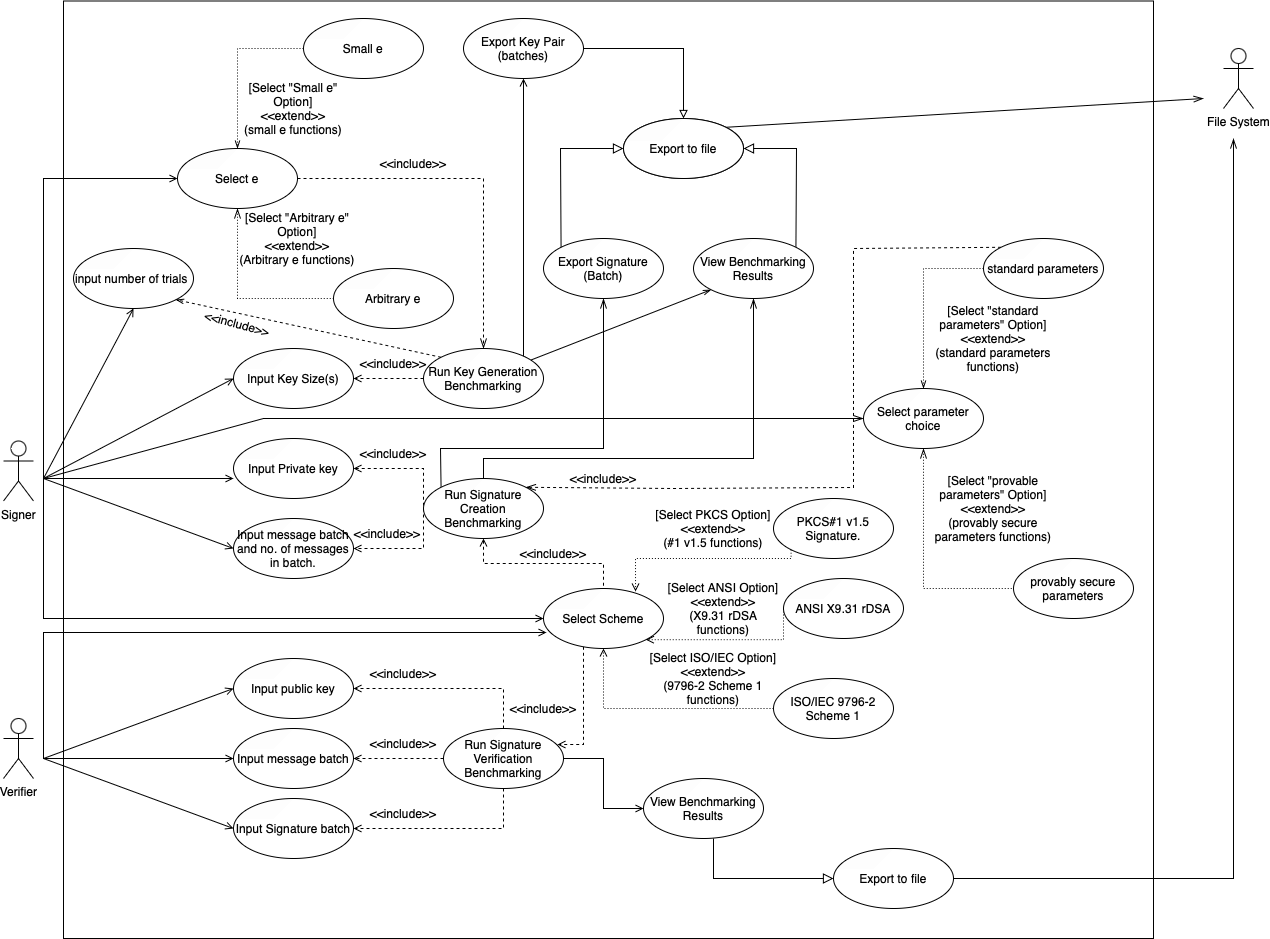
\includegraphics[scale=0.38]{poc_pictures/MAIN_USE-CASE.png}
    \caption{UML Use Case Diagram}
    \label{fig:uc}
\end{figure}



\textbf{Generate Keys Use Case}

\noindent\textbf{Flow of Events:}
\begin{enumerate}
    \item User selects "Generate Key" from the main menu options panel.
    \item User is presented with an input box prompting for the number of keys desired to be generated.
    \item User inputs desired number of keys into the box.
    \item System processes the request and updates the screen with the corresponding of number input boxes displayed vertically down the screen.
    \item System updates the screen with a checkbox labelled small e adjacent to each dynamically generated input box for each key.
    \item User inputs desired key sizes into each of the dynamically generated input boxes, additionally selecting the adjacent "small e" checkbox next to each input box where applicable.
    \item User is presented with an input box labelled enter number of trials for benchmarking run.
    \item User inputs desired number of trials into the box.
    \item System processes the request and completes the benchmarking run for the key generation process.
      \item System displays benchmarking results and notification informing the user that benchmarking process is complete.
      \item User is presented with options ”Export to file” for private key and public key batches corresponding to key pairs generated for all of their entered key configurations in one file.
        \item User is presented with options ”Export to file” for benchmarking results.
        \item User selects desired options for exporting.
\end{enumerate}

\noindent\textbf{Alternative flows:}
\begin{enumerate}
    \item[3a.] User inputs an invalid number of keys.
    \begin{enumerate}
        \item[3a1.] System warns user about the invalid input and prompts them to enter a valid number of keys.
    \end{enumerate}
        \item[4a.] System encounters an error during process of displaying the dynamically generated input boxes.
    \begin{enumerate}
        \item[4a1.] System displays an error message and prompts the user to try again.
    \end{enumerate}
    \item[6a.] User inputs an invalid key size into one of the dynamically generated input boxes.
    \begin{enumerate}
        \item[6a1.] System warns user about the invalid input and prompts them to enter a valid key size .
    \end{enumerate}
     \item[8a.] User inputs an invalid number of trials.
    \begin{enumerate}
        \item[8a1.] System warns user about the invalid input and prompts them to enter a valid number of trials.
    \end{enumerate}
        \item[9a.] System encounters an error during benchmarking of the key generation creation process.
    \begin{enumerate}
        \item[9a1.] System displays an error message and resets screen back to initial view.
    \end{enumerate}  
        \item[10a.]  User selected a small public exponent e for the entire key batch in step 6
    \begin{enumerate}
        \item[10a1.] System preloads provably secure key batches into signature creation and signature verification processes respectively.
    \end{enumerate}
\end{enumerate}



\textbf{Create Signature Use Case}

\noindent\textbf{Flow of Events:}
\begin{enumerate}
    \item User selects "Sign message" from the main menu options panel.
    \item User is presented with text boxes labeled "Input Private Key batch", "Input Message batch" and "Input no. of message".
    \item User provides all required inputs.
    \item User selects the desired signature scheme(s) to be used for benchmarking run from options ("PKCS\#1 v1.5 Signature", "ANSI X9.31 rDSA", ISO\slash IEC 9796-2 scheme 1).
      \item User is presented with radio button selection for Hash Function Size with the options labelled "Custom", "Provably Secure" and "Standard and underneath a drop down menu for selecting a concrete hash function"
        \item User selects "Standard" radio button as option for hash function size
         \item User is presented with solely fixed length hash functions in hash function drop down menu
          \item User selects hash function
          \item User initiates the signature creation benchmarking run by clicking relevant button.
  \item System processes the request and completes the benchmarking run for the signature creation process.
      \item System displays benchmarking results and notification informing the user that benchmarking process is complete.
      \item User is presented with options ”Export to file” for the resulting batch of computed signatures.
       \item User is presented with options ”Export to file” for benchmarking results.
       \item User selects desired options for exporting.
\end{enumerate}

\noindent\textbf{Alternative flows:}
\begin{enumerate}
     \item[2a.] Provably Secure public key batch was preloaded from key generation.
    \begin{enumerate}
     \item[2a1.] The system displays a visual indication that a provably secure private key batch has been preloaded.
    \item[2a2.] User is presented with text boxes labeled "Input Message batch" and "Input no. of message".
    \end{enumerate}
    \item[3a.] User inputs an invalid or mismatched private key batch.
    \begin{enumerate}
        \item[3a1.] System warns user about the invalid input and prompts them to enter a valid private key batch.
    \end{enumerate}
     \item[3b.] User inputs an invalid or mismatched message batch.
    \begin{enumerate}
        \item[3b1.] System warns user about the invalid input and prompts them to enter a valid message batch.
    \end{enumerate}
     \item[3c.] User inputs an invalid number of messages.
    \begin{enumerate}
        \item[3c1.] System warns user about the invalid input and prompts them to enter a valid number of messages.
    \end{enumerate}
         \item[5a.] Provably Secure public key batch was preloaded from key generation.
    \begin{enumerate}
     \item[5a1.] User is presented with radio button selection for instantiating scheme with provably secure parameters with the options labelled "yes", and "no" with currently selected option set to "yes".
    \item[5a2.]  User continues with currently selected yes option
        \begin{enumerate}
      \item[5a2a.] User selects "no" radio button as option for instantiating scheme with provably secure parameters.
    \begin{enumerate}
        \item[5a2a1.] Continue from step 5.
            \end{enumerate}
    \end{enumerate}
    \item[5a3.]  User is presented with radio button selection for Hash Function Size with a single option labelled "Provably Secure" this is currently selected and a drop down menu for selecting a concrete hash function"
     \item[5a4.]  Continue from step 6a1.
    \end{enumerate}
       \item[6a.] User selects "Provably Secure" radio button as option for hash function size
    \begin{enumerate}
        \item[6a1.] User is presented with solely variable length hash functions in hash function drop down menu
         \item[6a2.] The system sets the hash function output size to half the modulus length for each key.
    \end{enumerate}
         \item[6b.] User selects "Custom" radio button as option for hash function size
    \begin{enumerate}
        \item[6b1.] User is presented with solely variable length hash functions in hash function drop down menu
        \item[6b2.] The system prompts the user to input a custom hash size as a fraction e.g., 1/2.
         \item[6b3.] User enters custom hash size.
             \begin{enumerate}
             \item[6b3a.] User inputs invalid custom hash size.
    \begin{enumerate}
        \item[6b3a1.] System displays an error message and prompts the user to try again.
    \end{enumerate}
        \end{enumerate}
         \item[6b4.] The system sets the hash function output size to users specified fraction of modulus length for each key.
    \end{enumerate}
   

    \item[10a.] System encounters an error during benchmarking of the signature creation process.
    \begin{enumerate}
        \item[10a1.] System displays an error message and prompts the user to try again.
    \end{enumerate}
    \item[12a.]  User selected ISO\slash IEC 9796-2 scheme 1 in step 4.
    \begin{enumerate}
        \item[12a1.] User is presented with options "Export to file" for the computed batch of signatures and additionally if applicable a computed batch of non recoverable messages portions.
    \end{enumerate}
\end{enumerate}

\textbf{Verify Signature Use Case}

\noindent\textbf{Flow of Events:}
\begin{enumerate}
    \item User selects "Verify Signature" from the main menu options panel.
    \item User is presented with text boxes labeled "Input public Key batch", "Input Message batch" and "input signature batch".
    \item User provides all required inputs.
       \item User selects the desired signature scheme(s) to be used for benchmarking run from options ("PKCS\#1 v1.5 Signature", "ANSI X9.31 rDSA", ISO\slash IEC 9796-2 scheme 1).
      \item User is presented with radio button selection for Hash Function Size with the options labelled "Custom", "Provably Secure" and "Standard and underneath a drop down menu for selecting a concrete hash function"
              \item User selects "Standard" radio button as option for hash function size
         \item User is presented with solely fixed length hash functions in hash function drop down menu
          \item User selects hash function
               \item User initiates the signature verification benchmarking run by clicking relevant button.
         \item System processes the request and completes the benchmarking run for the signature verification process.
      \item System displays benchmarking results and notification informing the user that benchmarking process is complete.
      \item User is presented with options ”Export to file” for the results of signature verification for each and every message.
       \item User is presented with options ”Export to file” for benchmarking results.
       \item User selects desired options for exporting.
\end{enumerate}


\noindent\textbf{Alternative flows:}
\begin{enumerate}
     \item[2a.] Provably Secure public key batch was preloaded from key generation.
    \begin{enumerate}
     \item[2a1.] The system displays a visual indication that a provably secure private key batch has been preloaded.
    \item[2a2.] User is presented with text boxes labeled "Input Message batch" and "Input no. of message".
    \end{enumerate}
    \item[3a.] User inputs an invalid or mismatched private key batch.
    \begin{enumerate}
        \item[3a1.] System warns user about the invalid input and prompts them to enter a valid private key batch.
    \end{enumerate}
     \item[3b.] User inputs an invalid or mismatched message batch.
    \begin{enumerate}
        \item[3b1.] System warns user about the invalid input and prompts them to enter a valid message batch.
    \end{enumerate}
     \item[3c.] User inputs an invalid number of messages.
    \begin{enumerate}
        \item[3c1.] System warns user about the invalid input and prompts them to enter a valid number of messages.
    \end{enumerate}
         \item[5a.] Provably Secure public key batch was preloaded from key generation.
    \begin{enumerate}
     \item[5a1.] User is presented with radio button selection for instantiating scheme with provably secure parameters with the options labelled "yes", and "no" with currently selected option set to "yes".
    \item[5a2.]  User continues with currently selected yes option
        \begin{enumerate}
      \item[5a2a.] User selects "no" radio button as option for instantiating scheme with provably secure parameters.
    \begin{enumerate}
        \item[5a2a1.] Continue from step 5.
            \end{enumerate}
    \end{enumerate}
    \item[5a3.]  User is presented with radio button selection for Hash Function Size with a single option labelled "Provably Secure" this is currently selected and a drop down menu for selecting a concrete hash function"
     \item[5a4.]  Continue from step 6a1.
    \end{enumerate}
       \item[6a.] User selects "Provably Secure" radio button as option for hash function size
    \begin{enumerate}
        \item[6a1.] User is presented with solely variable length hash functions in hash function drop down menu
         \item[6a2.] The system sets the hash function output size to half the modulus length for each key.
    \end{enumerate}
         \item[6b.] User selects "Custom" radio button as option for hash function size
    \begin{enumerate}
        \item[6b1.] User is presented with solely variable length hash functions in hash function drop down menu
        \item[6b2.] The system prompts the user to input a custom hash size as a fraction e.g., 1/2.
         \item[6b3.] User enters custom hash size.
             \begin{enumerate}
             \item[6b3a.] User inputs invalid custom hash size.
    \begin{enumerate}
        \item[6b3a1.] System displays an error message and prompts the user to try again.
    \end{enumerate}
        \end{enumerate}
         \item[6b4.] The system sets the hash function output size to users specified fraction of modulus length for each key.
    \end{enumerate}
   
    \item[10a.] System encounters an error during benchmarking of the signature creation process.
    \begin{enumerate}
        \item[10a1.] System displays an error message and prompts the user to try again.
    \end{enumerate}
    \item[12a.]  User selected ISO\slash IEC 9796-2 scheme 1 in step 4.
    \begin{enumerate}
        \item[12a1.] The results of signature verification for each and every message in file offered for export, contains text corresponding to recovered portion of message if corresponding signature on message verified correctly.
    \end{enumerate}
\end{enumerate}





\subsection{Acceptance Tests}


\textbf{1. Benchmarking Key Pair Generation:}
\begin{enumerate}
\item Launch the benchmarking application and select "Generate Key" from the main menu.
\item Ensure the application presents an input box for entering the desired number of key pairs for generation.
\item Verify that after inputting the desired number of key pairs, the application dynamically displays corresponding input boxes for each key pair, along with a checkbox labeled 'small e' adjacent to each input box.
\item Check the functionality for the user to input desired key sizes into each dynamically generated input box and the option to select the 'small e' checkbox where applicable.
\item Confirm that the application presents an input box for entering the number of trials for the benchmarking run.
\item Test the process of inputting the desired number of trials and verify that the system processes the request correctly.
\item Inspect the system's ability to complete the benchmarking run for the key generation process without errors or exceptions.
\item Ensure the application displays benchmarking results along with a notification confirming the completion of the benchmarking process.
\item Verify the availability and functionality of the options to export both the most recently benchmarked private and public key batches, as well as the benchmarking results to a file.
\end{enumerate}


\textbf{2. Benchmarking Signature Generation:}
\begin{enumerate}
    \item Navigate to the signature generation section in the application.
    \item Use the option to import a valid message batch.
    \item Use the option to import a valid private key batch.
    \item Check that the application notifies the user if an empty message batch or an invalid private key batch is provided, with instructions to provide valid inputs.
    \item Confirm that the application allows the user to select "Standard", "Provably Secure" or "custom" hash function size.
    \item When "Standard" is selected, verify that only fixed-length hash functions are available for selection.
    \item When "Provably Secure" is selected, verify that variable-length hash functions are available and that the hash function output size is automatically set to half the modulus length for each key.
    \item Ensure the benchmarking of the signature creation process completes without errors.
    \item Confirm the application provides notification upon successful completion of the benchmarking process.
    \item Verify that options to export the generated signatures and benchmarking results are available and functional.
\end{enumerate}

\textbf{2. Benchmarking Signature Generation (Alternative Scenarios):}

\begin{itemize}
    \item If a provably secure private key batch was preloaded prior to navigating to signature generation:
    \begin{enumerate}
        \item Verify that the application indicates that the key batch has been preloaded.
        \item Confirm that the hash function selection is limited to "Provably Secure" options.
    \end{enumerate}
    \item When the "Custom" hash function size is selected:
    \begin{enumerate}
        \item Ensure that the user is prompted to input a custom hash size as a fraction.
        \item Check that an error is displayed if the user inputs an invalid custom hash size, with an option to retry.
    \end{enumerate}
\end{itemize}


\textbf{3. Benchmarking Signature Verification:}
\begin{enumerate}
    \item Navigate to the signature Verification section in the application.
    \item Use the option to import a valid message batch.
    \item Use the option to import a valid public key batch.
    \item Check that the application notifies the user if an empty message batch or an invalid public key batch is provided, with instructions to provide valid inputs.
    \item Confirm that the application allows the user to select "Standard", "Provably Secure" or "custom" hash function size.
    \item When "Standard" is selected, verify that only fixed-length hash functions are available for selection.
    \item When "Provably Secure" is selected, verify that variable-length hash functions are available and that the hash function output size is automatically set to half the modulus length for each key.
    \item Ensure the benchmarking of the signature creation process completes without errors.
    \item Confirm the application provides notification upon successful completion of the benchmarking process.
\item Verify options to export both the generated signature verification results and benchmarking results to a file.
\end{enumerate}

\textbf{3. Benchmarking Signature Verification (Alternative Scenarios):}

\begin{itemize}
    \item If a provably secure public key batch was preloaded prior to navigating to signature verification:
    \begin{enumerate}
        \item Verify that the application indicates that the key batch has been preloaded.
        \item Confirm that the hash function selection is limited to "Provably Secure" options.
    \end{enumerate}
    \item When the "Custom" hash function size is selected:
    \begin{enumerate}
        \item Ensure that the user is prompted to input a custom hash size as a fraction.
        \item Check that an error is displayed if the user inputs an invalid custom hash size, with an option to retry.
    \end{enumerate}
\end{itemize}





\textbf{4. Benchmarking Signature Creation and Verification with PKCS\#1 v1.5:}
\begin{enumerate}
\item Select the PKCS\#1 v1.5 Signature Scheme for benchmarking within the application.
\item Conduct benchmarking of both the signature generation and verification processes with corresponding test batches using the previous steps. Ensure both processes succeed.
\item Verify the functionality to export the benchmarking results for both signature generation and verification processes to a file.
\item Verify the functionality to export the results for the actual verification of signatures to a file.
\end{enumerate}


\textbf{5. Benchmarking Signature Creation and Verification with ANSI X9.31 rDSA:}
\begin{enumerate}
\item Select the ANSI X9.31 rDSA Signature Scheme for benchmarking within the application.
\item Conduct benchmarking of both the signature generation and verification processes with corresponding test batches using the previous steps. Ensure both processes succeed.
\item Verify the functionality to export the benchmarking results for both signature generation and verification processes to a file.
\item Verify the functionality to export the results for the actual verification of signatures to a file.
\end{enumerate}


\textbf{6. Benchmarking Signature Generation with ISO/IEC 9796-2:2010 Scheme 1:}
\begin{enumerate}
\item Set the application to use the ISO/IEC 9796-2:2010 Signature Scheme 1.
\item Conduct benchmarking of  the signature generation process with corresponding test batches using the previous steps and ensure it succeeds.
\item Verify options to export a batch of messages to a file (e.g., as a message recovery mode, non recoverable portion of messages is transmitted along with signature).
\end{enumerate}

\textbf{7. Benchmarking Signature Verification with ISO/IEC 9796-2:2010 Scheme 1:}
\begin{enumerate}
\item Select the ISO/IEC 9796-2:2010 Scheme 1 for benchmarking within the application.
\item Conduct benchmarking of both the signature generation and verification process with corresponding test batches using the previous steps. Ensure both processes succeed.
\item Verify the functionality to export the benchmarking results for the signature verification process to a file.
\item Verify the functionality to export the results for the actual verification of signatures to a file.
\item Check that results for the actual verification of signatures additionally contain recovered message portions.
\end{enumerate}


\section{Appendix B.2 Design}

\textbf{Design of Signature Model Assembly}
\begin{figure}[H]
    \centering
    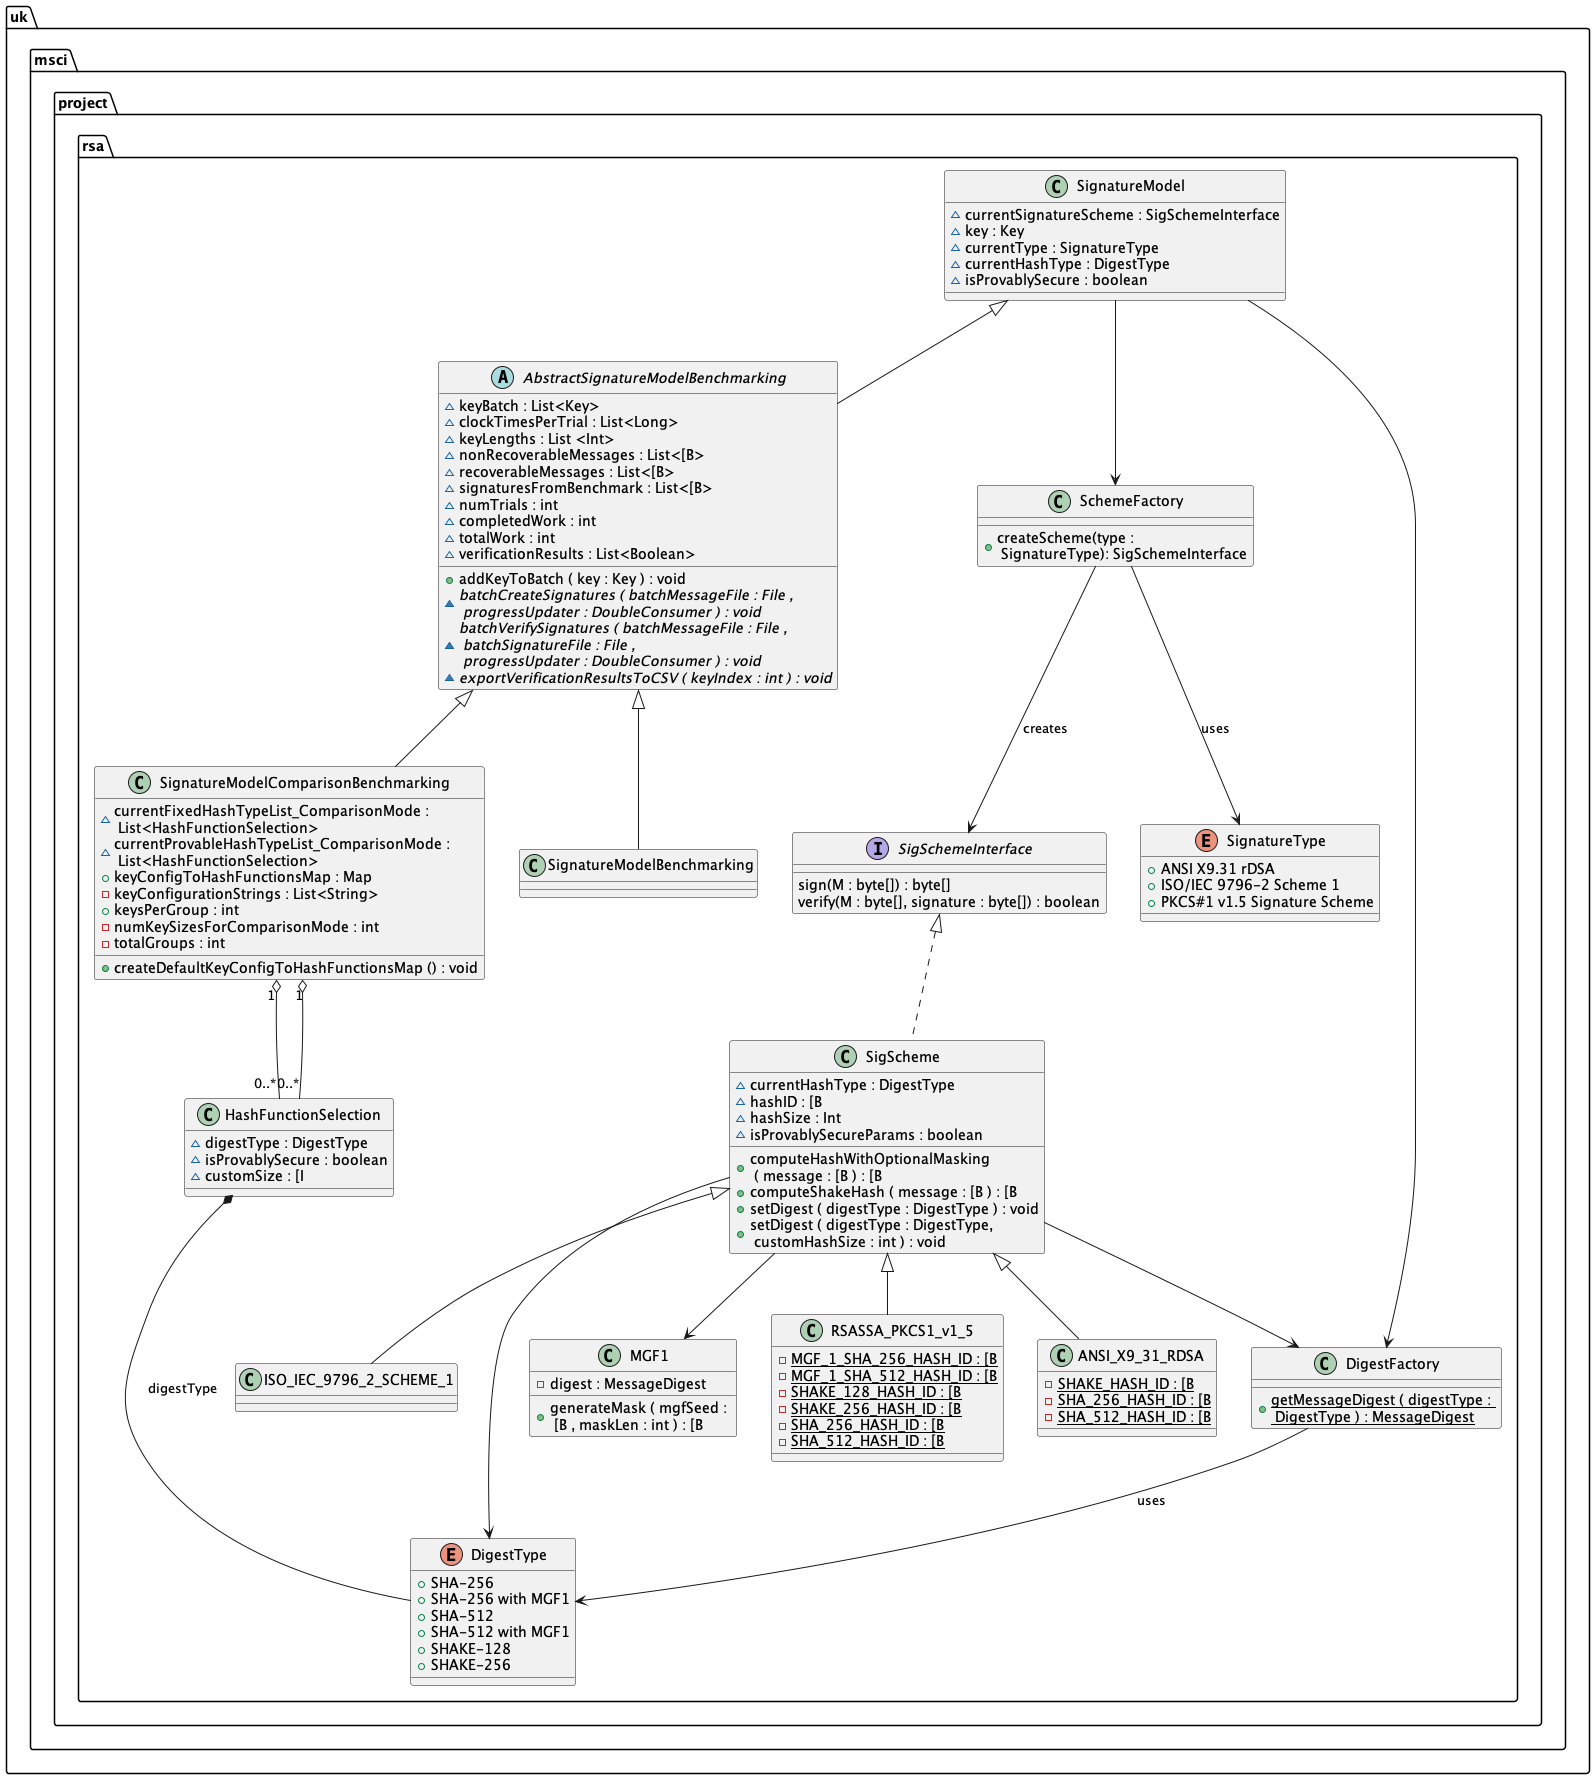
\includegraphics[scale=0.335]{main_pictures/signatureModel.png}
    \caption{Design of Signature Model Assembly}
    \label{fig:SIGMODDESIGN}
\end{figure}

Central to this assembly is the SignatureModel class. It holds the state of a user-initiated digital signature scheme, including the current signature scheme, the associated key, and the digest type. 

Building upon the SignatureModel, the AbstractSignatureModelBenchmarking class extends its capabilities by integrating benchmarking functions. It maintains lists to store trial times, benchmarked signatures, and captures recoverable and non-recoverable parts of messages where applicable

The SignatureModelBenchmarking subclass specialises in conducting batch operations in benchmarking scenarios. This class is designed for efficiency in large-scale data handling by utilising concurrency, managing multiple keys, and processing large volumes of signatures simultaneously.

The SignatureModelComparisonBenchmarking class offers a specialised form of benchmarking to be described as cross-parameter comparison mode. It is designed to extend benchmarking functionality to accommodate comparison benchmarking allowing for the side-by-side evaluation of parameter types for a provided signature scheme. This class is structured to manage and benchmark various key sizes and hash function. It maintains further lists for application on a per key size basis to store keyConfigurationStrings that each uniquely represent a key parameter configuration and a keyConfigToHashFunctionsMap, a mapping that associates each group of key configurations with their respective hash functions. 

\textbf{Factory pattern}

The factory pattern manifests within this assembly through the SchemeFactory class, which simplifies the instantiation of various RSA signature schemes like ANSI X9.31 and ISO/IEC 9796-2. By following the SigSchemeInterface, every signature scheme adheres to a uniform set of operations, ensuring consistency across different implementations.

The DigestFactory pattern, mirrors the factory design of the signature schemes, serves a similar function for hash functions. It encapsulates the complexity of algorithm instantiation, guided by the DigestType. This separation of concerns promotes a clean architecture, allowing for straightforward extensions and modifications.

During the instantiation of a signature scheme with provably secure parameters, the DigestFactory pattern plays a facilitatory role. When a scheme is instantiated with the flag for provably secure parameters set the DigestFactory aids in configuring the MessageDigest to the specified DigestType, adjusting the hash size accordingly (hash function output size of half the modulus length to achieve provable security).

\newpage
\subsection{Key Generation Module}

\textbf{Design of Key Generation Controller Assembly: Orchestration of key generation}

\begin{figure}[H]
    \centering
    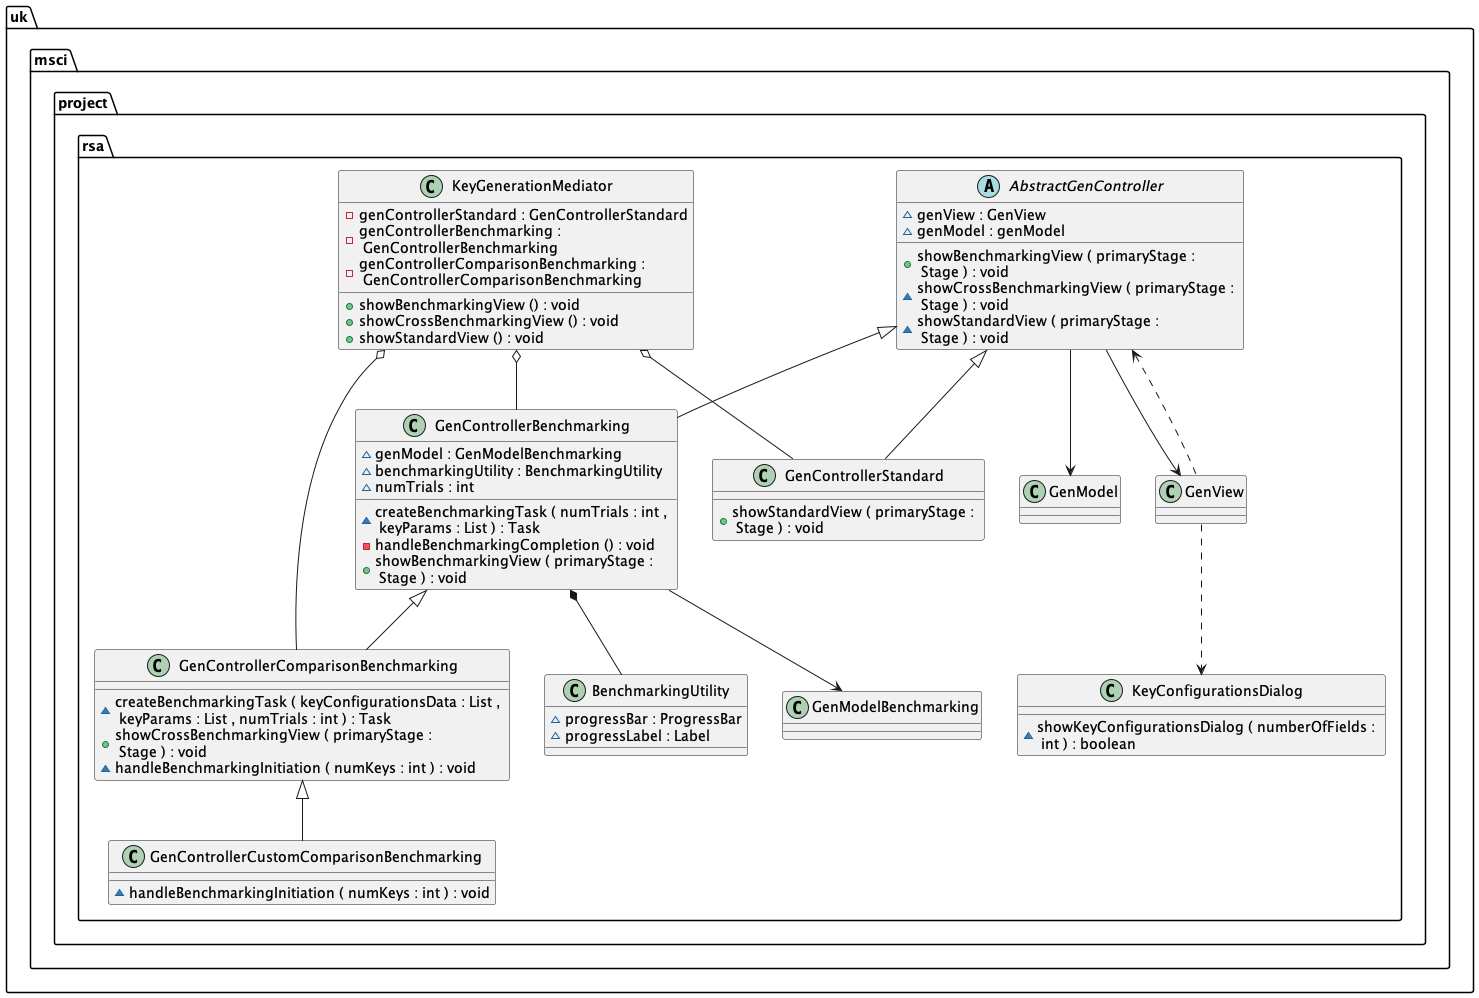
\includegraphics[scale=0.367]{main_pictures/genController.png}
    \caption{Design of Key Generation Controller Assembly: Orchestration of key generation}
    \label{fig:KEYCONTROLLERDESIGN}
\end{figure}

\textbf{KeyGenerationMediator:}

Central to the Key Generation module is the KeyGenerationMediator, serving as the intermediary between the primary MainController and the distinct key generation controllers. The mediator pattern comes into play, facilitating the management of various key generation operational modes—standard, benchmarking, and comparison benchmarking—without overcomplicating the main controller's logic. This mediator ensures that appropriate controllers are activated and configured to match the operational context, whether the user is generating a single key pair or a batch for benchmarking purposes.

\textbf{Controllers:}

The GenControllerBenchmarking class is tailored for benchmarking key generation performance, holding a reference to the GenModelBenchmarking and a BenchmarkingUtility with a ProgressBar for real-time progress indication. It can create tasks for generating keys under given parameters and handle the completion of these tasks, updating the view to reflect results.

The GenControllerStandard is focused on standard, non-benchmarked key generation processes. It provides a straightforward interface to generate keys and output them to the user, signifying a successful operation without the need for analysis.

The GenControllerComparisonBenchmarking in a similar intuition to its signature module equivalent extends benchmarking functionality to accommodate the side-by-side evaluation of key configuration types. This class can initiate benchmarking tasks that compare different parameter type groupings, providing insights into performance differentials between various key configurations at scale for arbitrary key sizes.

In support of the controllers, the GenModel and its subclass GenModelBenchmarking serve as the data models for key generation. They encapsulate the state and logic for key generation operations, providing a structured approach to manage and store generated keys and related data.


\textbf{Design of the Key Generation Model Assembly}


\begin{figure}[H]
    \centering
    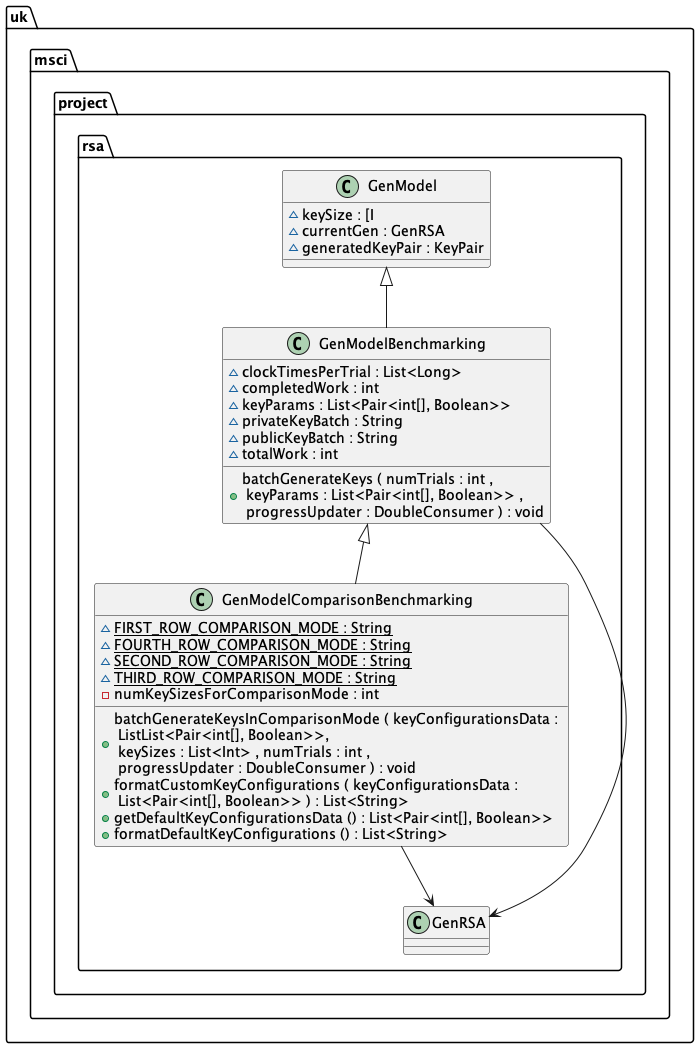
\includegraphics[scale=0.39]{main_pictures/genModel.png}
    \caption{Design of the Key Generation Model Assembly}
    \label{fig:KEYMODEDESIGN}
\end{figure}

The GenModel class encapsulates the attributes and behaviours necessary for RSA key generation, including the key size, the current key generation instance (currentGen), and the resultant KeyPair (generatedKeyPair). This class represents the state of a user-initiated RSA key generation process and provides a foundation for more specialised key generation models.

The GenModelBenchmarking class extends the GenModel to support the benchmarking of RSA key generation. It contains lists for tracking execution times (clockTimesPerTrial) and maintains state related to the key generation process, such as completed and total work indicators. It also holds the key configuration parameters (keyParams) for benchmarking by key size, and the batches of private and public keys generated during benchmarking (privateKeyBatch, publicKeyBatch). This class is responsible for initiating batch RSA key generation tasks, to utilised for performance assessment across various key configurations for specified key sizes.

The GenModelComparisonBenchmarking class further specialises the benchmarking process. It introduces additional attributes for managing comparison modes, such as strings representing the default configuration modes and an integer for the number of key sizes under comparison (numKeySizesForComparisonMode). This class is equipped to perform key generation with user-specified parameters, facilitating direct comparisons between different sets of key configurations. This allows for the evaluation of standard vs. provably secure parameters and user-defined custom parameter sets.



\begin{landscape}
\subsection{Results Module}
\pagestyle{empty}%
\begin{figure}[h]
    \centering
    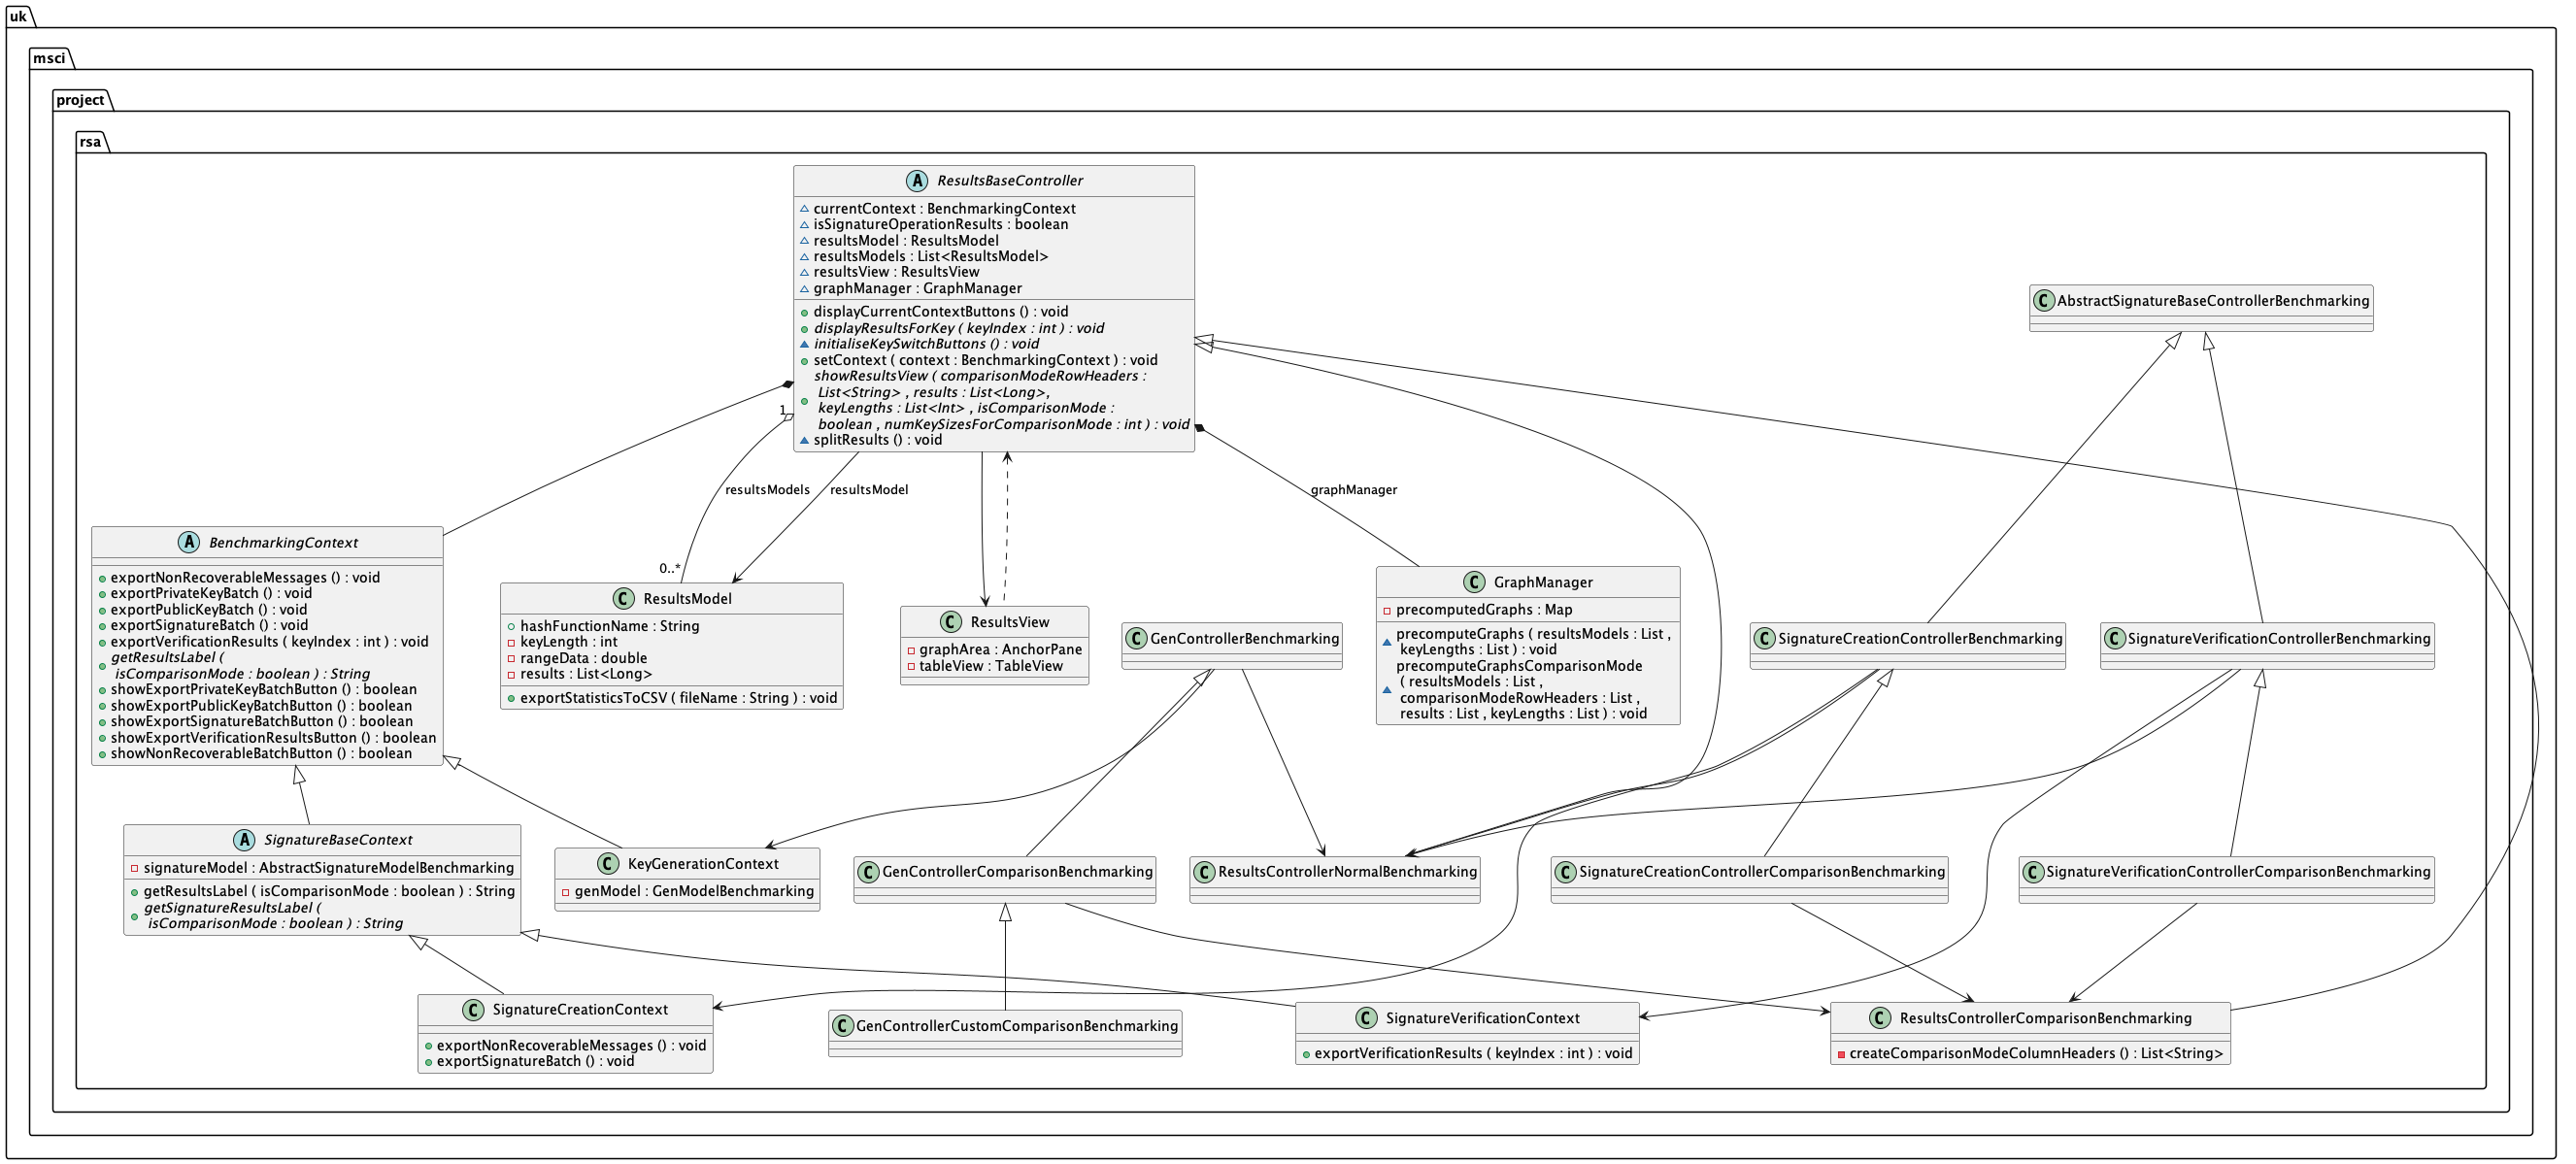
\includegraphics[scale = 0.263]{main_pictures/results.png}
    \caption{Design of the Results Module}
    \label{fig:RESULTSMODULEDESIGN}
\end{figure}
\end{landscape}

The Results Module is designed to process and present the outcome of benchmarking activities. Its core components, the ResultsModel and Results controller assembly, interact to store and manage statistical data, offering insights into the performance of the considered digital signature schemes and/or key generation processes aggregated by key size (e.g., multiple key configurations per each in comparison mode) or by key (in normal benchmarking). 

The ResultsModel serves as the data repository and records an array of time measurements from benchmarking trials, subsequently computing statistical averages like mean, median and percentile values. It is equipped with methods for export functionalities to output the gathered data to CSV files for further use or examination.

The ResultsBaseController, an abstract class, lays the foundation for controllers that manage results display logic. This class holds references to a list of ResultsModel instances, thus supporting the representation of benchmarking results for individual keys. It orchestrates the interaction between the results view and model components, and it provides methods for the initial setup of the results context, display logic for the current benchmarking context, and splitting results for different key configurations.

Inheriting from ResultsBaseController are two specialised controllers: ResultsControllerNormalBenchmarking and ResultsControllerComparisonBenchmarking, each tailored to a specific mode of benchmarking. The ResultsControllerNormalBenchmarking focuses on results related to individual keys. It simplifies the presentation of benchmarking data by concentrating on one key at a time, providing a streamlined and detailed view of its performance metrics. On the other hand, ResultsControllerComparisonBenchmarking is designed for comparison benchmarking mode, facilitating the juxtaposition of performance metrics across different key configurations in their groups and associated group hash functions by key size if results relate to signature operations.

The Results Module integrates with the overarching BenchmarkingContext to ensure that the results displayed are contextually relevant. The BenchmarkingContext and its subclasses manage the visibility of UI components relevant to each benchmarking scenario.

The Results Controller assembly encapsulates a GraphManager responsible for creating and handling various graphical representations of the benchmarking results. It supports different graph types like histograms, box plots, and line graphs, which can be used to visualise the results in both individual key analysis (normal benchmarking mode) and comparative analysis across different key sizes and configurations.




\begin{landscape}
\subsection{UML Package Diagram (All functionality)}
\pagestyle{empty}

\begin{figure}[H]
    \centering
    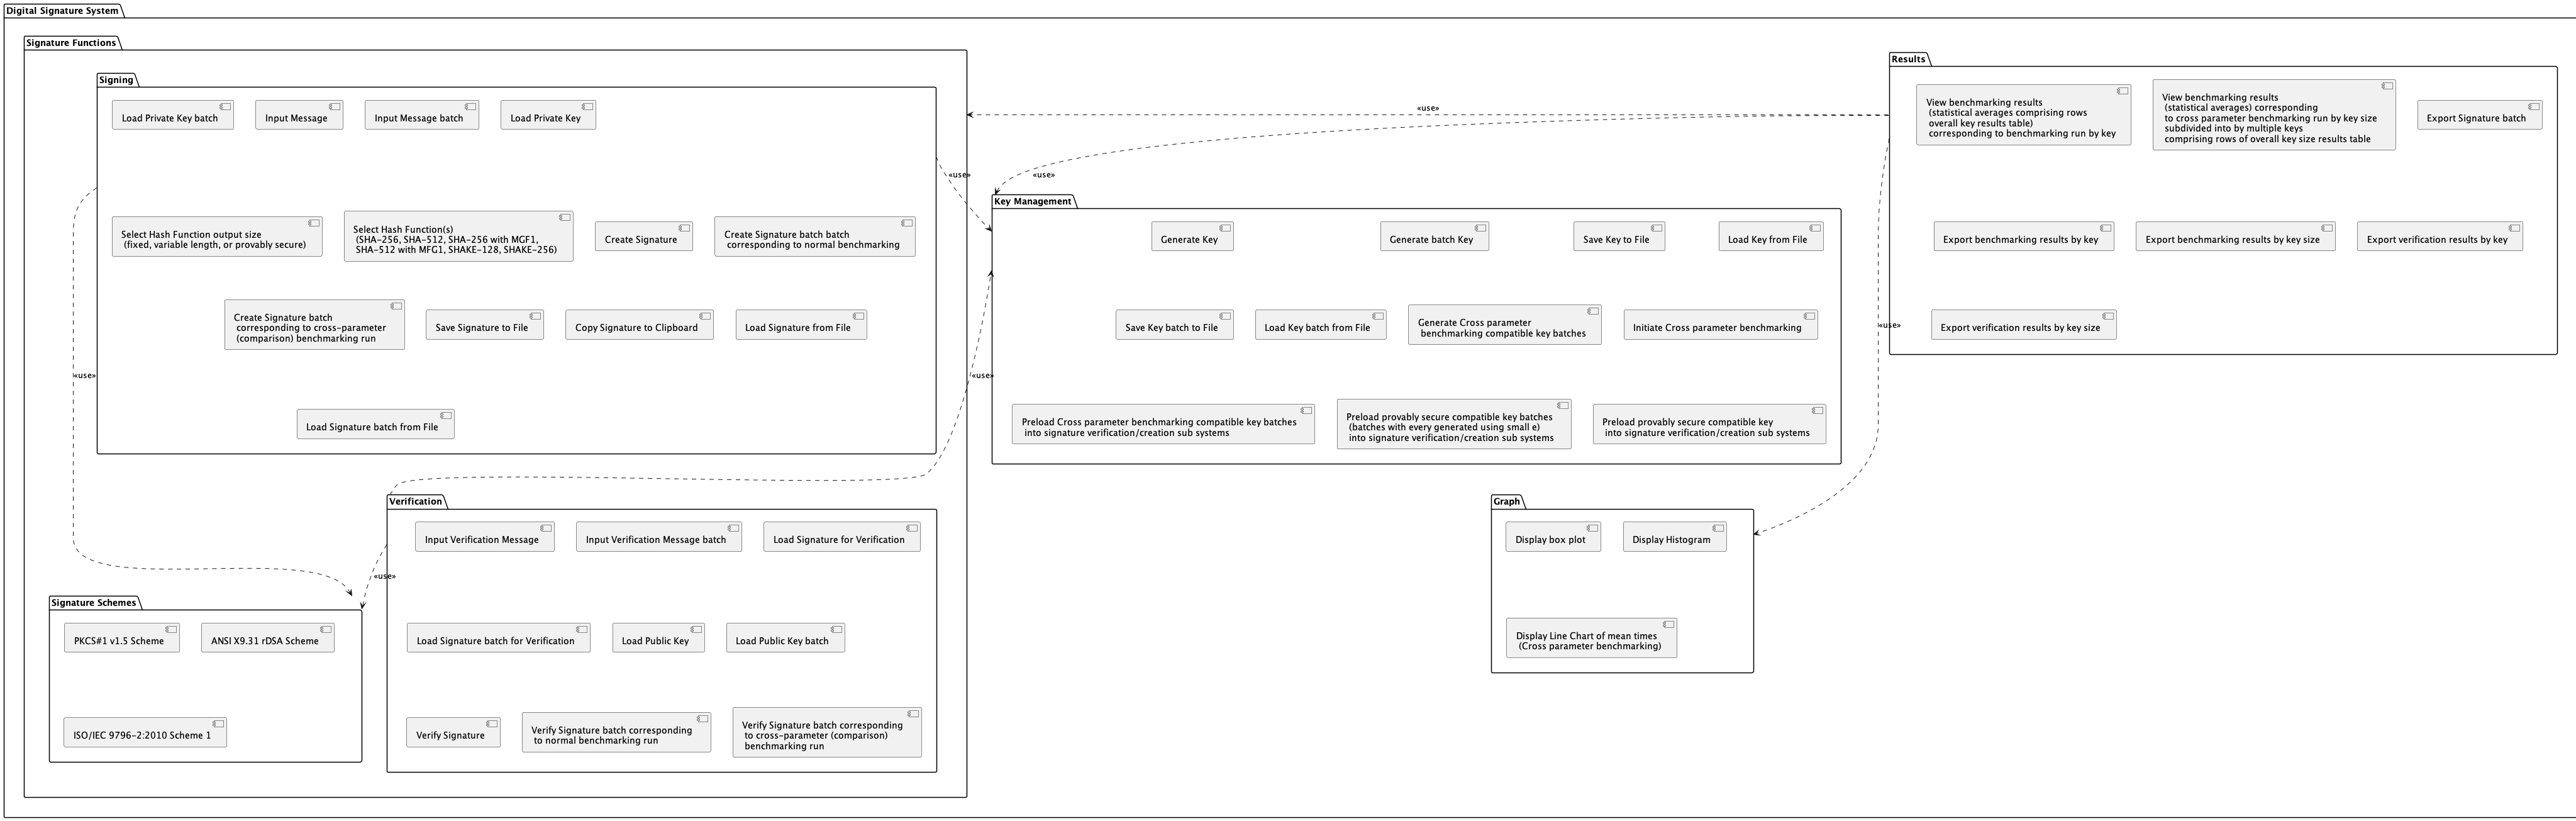
\includegraphics[width=1.1\linewidth]{main_pictures/package.png}
    \caption{UML Package Diagram (All functionality)}
    \label{fig:pack}
\end{figure}
\end{landscape}


Figure \ref{fig:pack} depicts the functionality of the program and is in direct alignment with the full feature set of program as specified across the both the essential and non-essential requirements.

The "Key Management" package is a suite encompassing all key-related operations. It allows for generating individual and batch keys, saving and loading these keys to and from files, and managing keys for cross-parameter benchmarking. It also handles the preloading of keys for signature processes where applicable. For example batches generated using a small public exponent i.e., "provably secure compatible key batches" can be preloaded into signature processes. Additionally in comparison benchmarking mode, it allows users to enter desired key sizes and automatically generates keys for each inputted key size based the 2 groups of key configurations respective to standard and provably secure parameters in sequential order comprising the public-private key batch pairing. This is what can be described as Cross parameter benchmarking compatible key batches and they are preloaded into signature verification/creation sub systems. In Custom comparison mode, keys for each key size can be generated based on arbitrary groups of key configurations (and the hash functions to be used for each group) selected by the user.

Within the "Signature Functions" package, sub-packages are dedicated to signing and verification tasks. They incorporate user inputs, key management, and hash function selection, each tailored to support the considered signature schemes presented in a separate sub-package, including PKCS\#1 v1.5, ANSI X9.31 rDSA, and ISO/IEC 9796-2:2010 Scheme 1. Within standard benchmarking, a singular hash function is selected for uniform application across all key configurations. Cross-parameter benchmarking introduces a divergent selection of hash functions, with fixed-length options (SHA-256 and SHA-512) for standard parameters and variable-length options (SHAKE-128 and SHAKE-256) configured with a hash output of half the length of the modulus  for each key it used with for provably secure parameters. Custom comparison benchmarking forgoes the need for discrete hash function choices during the signature phase by preloading selections during the key generation phase e.g., hash function selections for each group of custom key configurations specified by a user are entered during key generation when the group is defined obviating the need for the user to provide a selection during the signature phase.

The "Results" package deals with the presentation and export of benchmarking outcomes. It ensures the user can view and export benchmarking results by key (normal benchmarking) or by key size (comparison benchmarking),
Lastly, the "Graph" package offers a visual representation of statistical data. It contains functionality to display box plots, histograms, and line charts, particularly useful for cross-parameter benchmarking results, enhancing the user's understanding of the data.


\textbf{Benchmarking Modalities}

\begin{itemize}
    \item \textbf{Normal Benchmarking}: The system provides a straightforward assessment of the relevant process, offering the user key-specific benchmarking results. For signature operations, the same hash function is applied to every key configuration.
     \item \textbf{Comparison Benchmarking (Standard vs. Provably Secure)}: This mode offers a direct comparative analysis between standard and provably secure key configuration groups (with user selected hash functions for each group). This allows evaluation of the performance of the Standard and Provably Secure groupings, with all trials repeated for every hash function and key configuration combination for each group. Results are then presented side by side in a table and/or overlaid graphs for each entered key size. 
     \item \textbf{Custom Comparison Benchmarking}: In this mode, users have the flexibility to specify key configurations and corresponding hash functions for each group. They can then assess the performance of their chosen key configuration groupings, with all trials repeated for every hash function and key configuration combination for each group. Results are presented side by side in a table and/or overlaid graphs for each entered key size.
\end{itemize}

Dependencies between these packages indicate a flow of data and usage across the system. For example, the "Results" package uses data generated by "Signature Functions" and "Key Management," and also utilises the "Graph" package for displaying results, signifying a cohesive and interrelated system design.


\subsection{UML sequence diagrams (Normal Benchmarking functionality only)}
\begin{figure}[H]
    \centering
    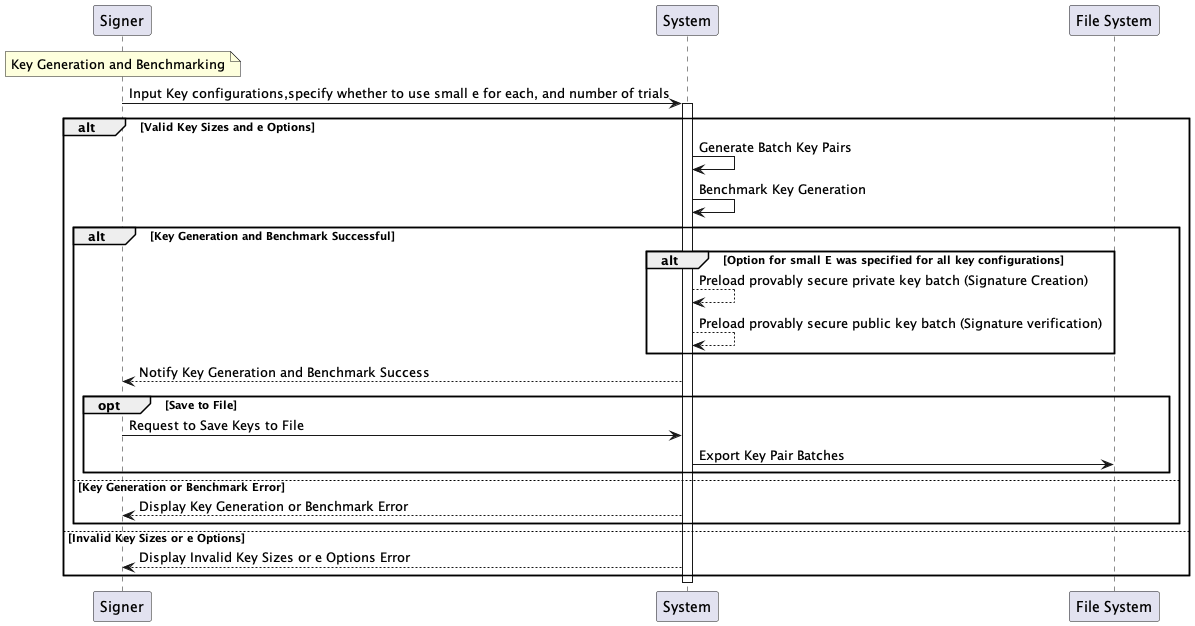
\includegraphics[scale=0.42]{main_pictures/sequenceKey.png}
    \caption{UML Sequence Diagram (Key Generation)}
    \label{fig:uc}
\end{figure}

The above diagram outlines the steps taken by a user within the system to configure and execute the key generation process, which is critical for both the signature creation and verification phases.

The process begins when the user inputs the key configurations, indicating the desired key size and whether to utilise a small public exponent (e) for each key. The system then proceeds to generate a batch of key pairs and benchmarks the key generation process, provided the key sizes and options are valid. An alternate path allows for the preloading of provably secure key batches if the option for a small e was specified for all key configurations,

Upon successful completion, the user is notified, benchmarking results are displayed and there is an option to save the generated keys to a file. This action interacts with the file system to persist the key batches. Should there be an error during key generation or benchmarking, or if the provided key sizes or options are invalid, the system displays the appropriate error message.

\begin{figure}[H]
    \centering
    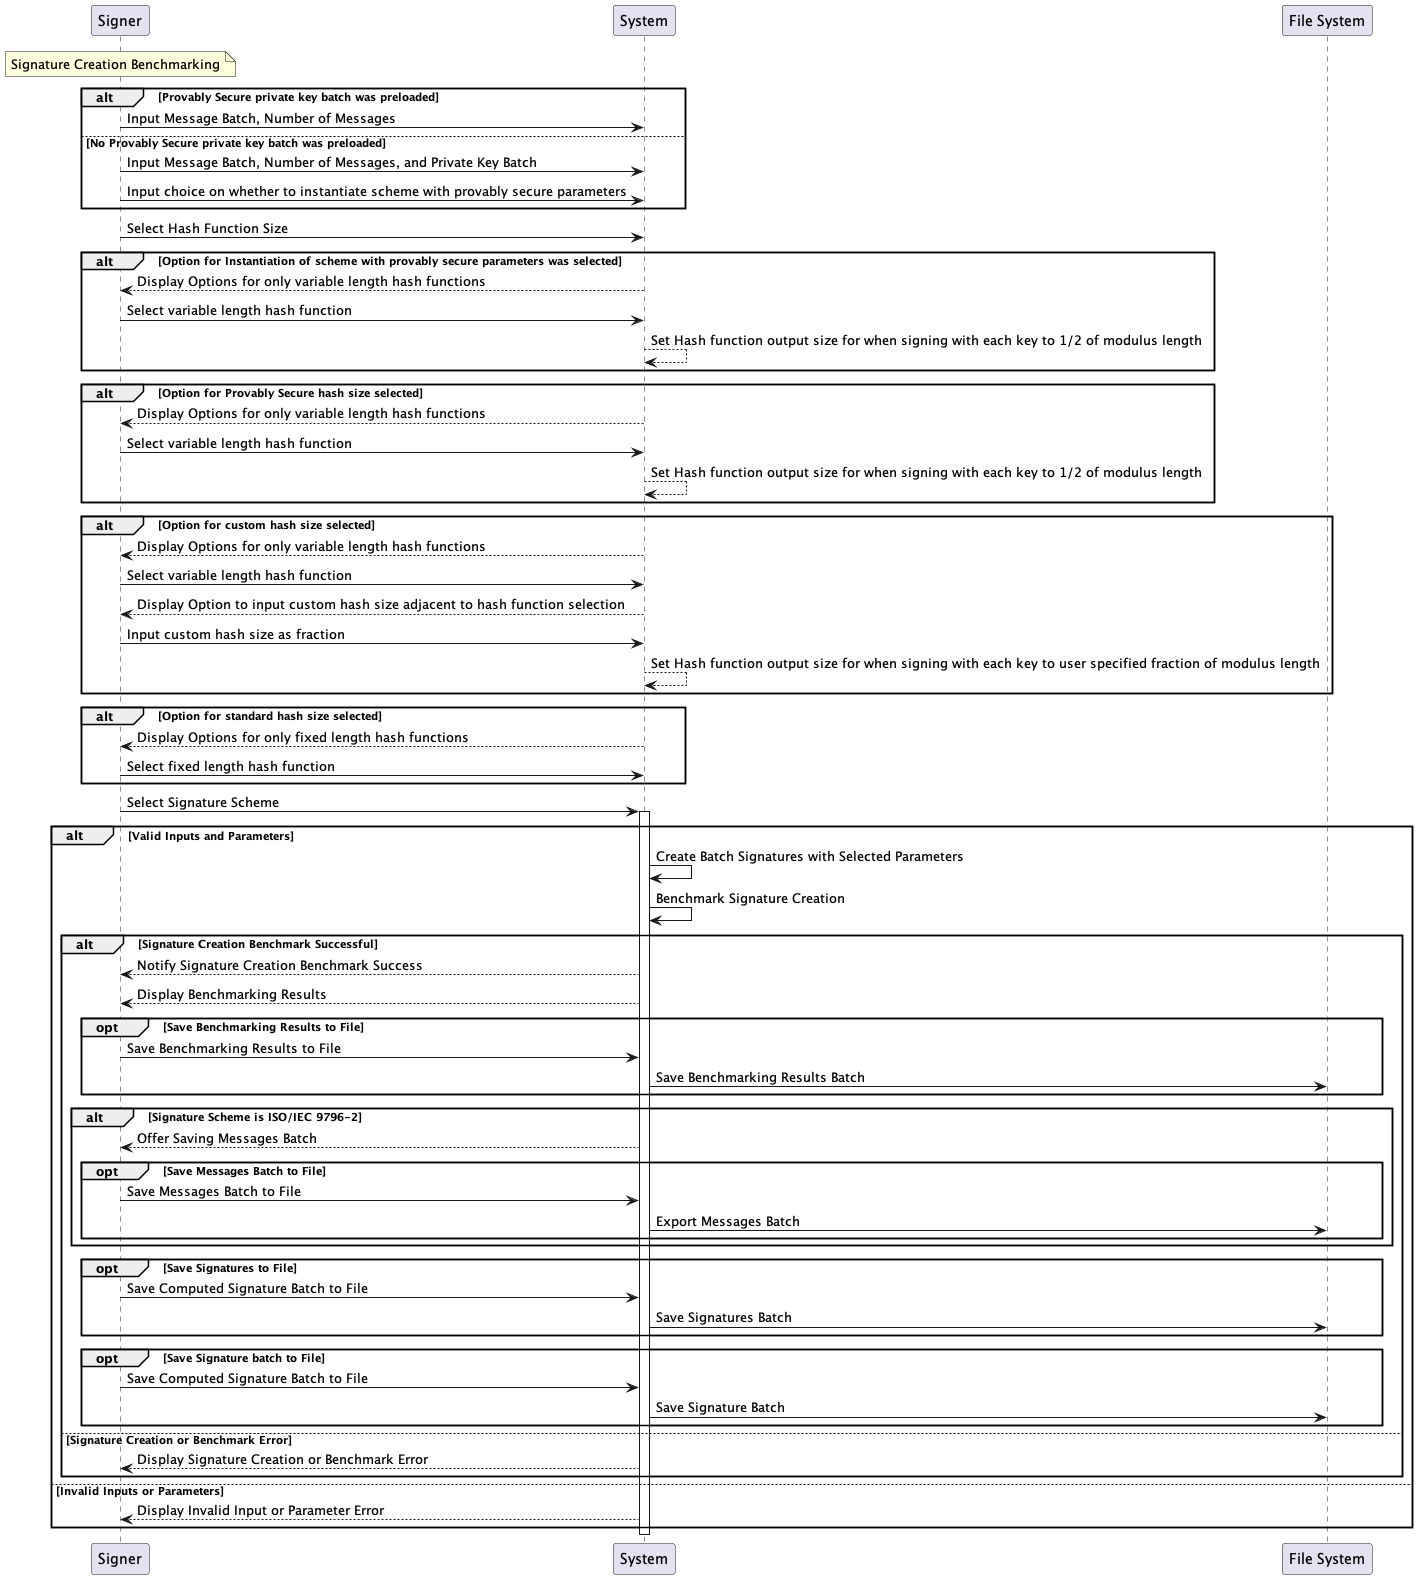
\includegraphics[scale=0.34]{main_pictures/sequenceSign.png}
    \caption{UML Sequence Diagram (Signature Creation)}
    \label{fig:uc}
\end{figure}

The Signature Creation sequence diagram portrays the steps for digital signature generation. The sequence begins with a potential bypass: if a provably secure public key batch was preloaded—contingent upon the selection of a small public exponent e for the entire key batch during the Key Generation phase—the system obviates the need for the user to provide a private key batch.
The system presents the hash function selection as a decision point:
\begin{itemize}
    \item \textbf{Provably Secure Parameters}: If the option for instantiation with provably secure parameters is selected, the system displays only the variable length hash functions. After the user selects one, the system sets the hash function output size to half the modulus length for each key.
    \item \textbf{Provably Secure Hash Size}: If the user opts for a provably secure hash size, the system again displays only variable length hash functions. Upon selection, the output size is configured to half of the modulus length, aligning with provable security standards.
    \item \textbf{Custom Hash Size}: When a custom hash size is chosen, the user is presented with variable length hash functions. The system then prompts the user to input a custom hash size as a fraction, which it uses to determine the hash function output size in relation to the modulus length of each key.
    \item \textbf{Standard Hash Size}: If the standard hash size is preferred, the system limits the display to fixed length hash functions, from which the user can select.
\end{itemize}

Finally, the user selects a message batch and a signature scheme , completing the setup for signature generation. Following these selections, the system generates a batch of signatures and benchmarks their creation. It then provides the user with the results, including options to save the generated signatures and the benchmarking statistics. 

In the Signature Creation sequence, specialised functionality comes into play when implementing message recovery signature schemes such as the ISO/IEC 9796-2 Scheme 1. These schemes require special consideration because their behaviour differs from the standard digital signature process. The ISO/IEC 9796-2 schemes incorporate message recovery features, where part or all of the original message can be reconstructed from the signature itself. This necessitates additional logic in the signing process. The system offers export for a non-recoverable message batch in such cases where each entry is preceded by a "1" if a non-recoverable message follows, whereas a "0" flag denotes the absence of such a message part.


\begin{figure}[H]
    \centering
    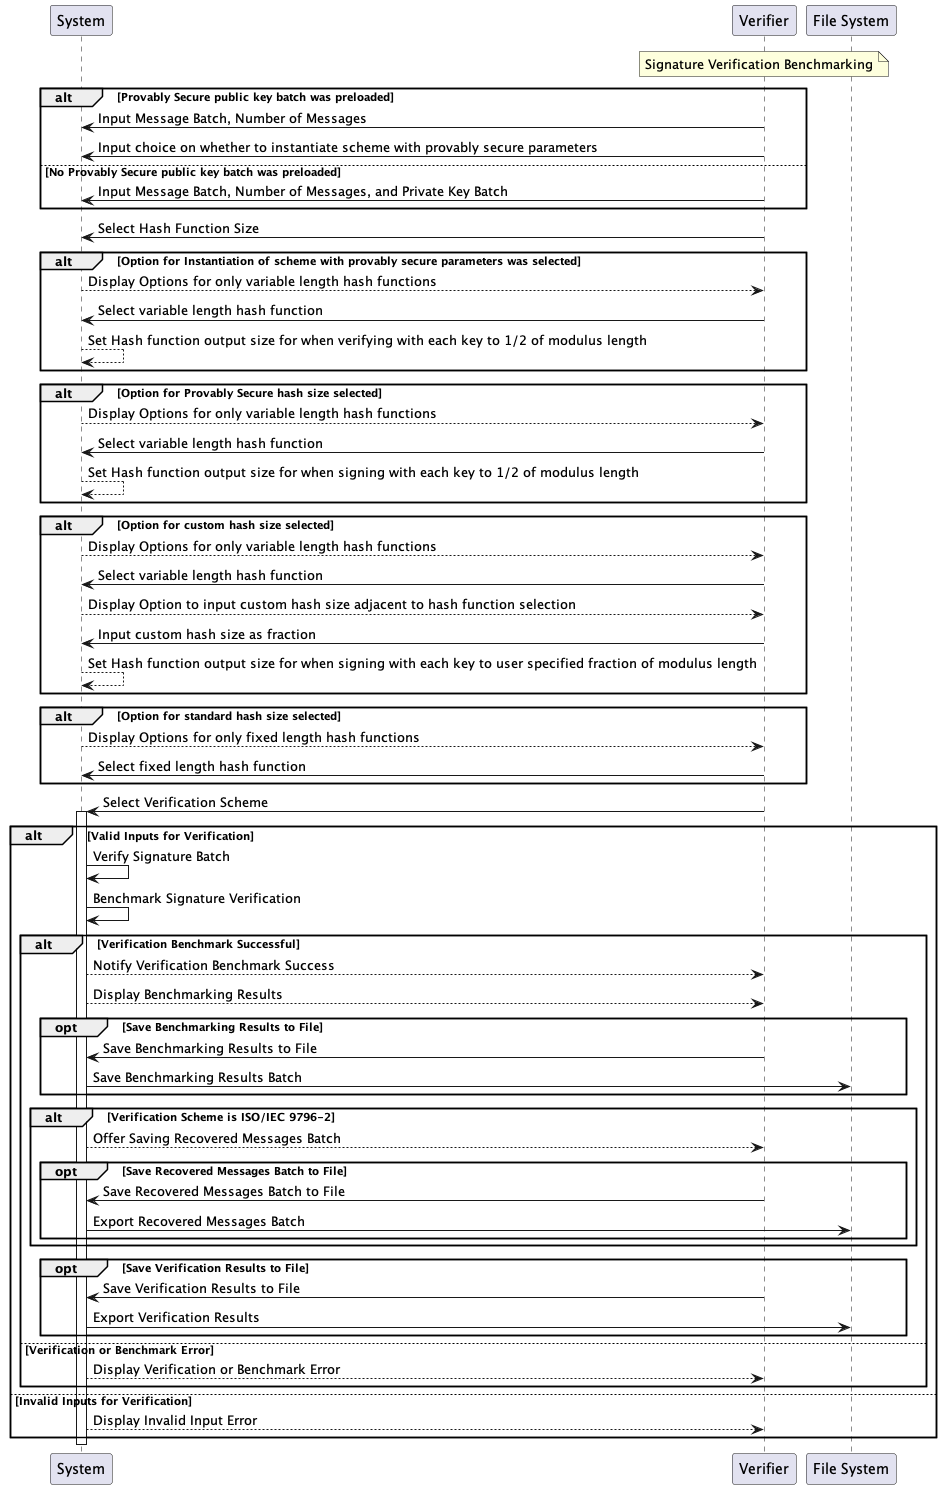
\includegraphics[scale=0.4]{main_pictures/sequenceVerify.png}
    \caption{UML Sequence Diagram (Signature Verification)}
    \label{fig:uc}
\end{figure}

The Signature Verification sequence diagram portrays the steps for digital signature verification. The sequence begins with the same potential bypass relating to the preload of a key batch (but this time around for a public key batch) i.e.,  if a provably secure public key batch was preloaded the system obviates the need for the user to provide a public key batch.
As with signature creation, the user encounters the equivalent decision point regarding hash function size hash function selection:

Following this the user then selects a message batch and a signature scheme, completing the setup for signature generation. Following these selections, the system generates a batch of signatures and benchmarks their creation. It then provides the user with the results, including options to save the generated signatures and the benchmarking statistics. 

For signatures associated with message recovery i.e., ISO/IEC 9796-2 Scheme 1, the sequence accommodates a vital step where the message batch inputted by the verifier should be the non recoverable message batch file exported after the conclusion of the signature creation benchmarking. Such a file contains entries (corresponding to signatures in a one-to-one line by line basis) starting with a "1" or "0" flag to indicate the presence or absence of non-recoverable message parts. The system will then use the non recoverable part when applicable for a signature entry to generate the contents of a recovered message batch which is offered as part of the verification results export.





 

\section{Appendix B.3 Testing}

\subsection{Appendix B.3A Integration Testing}
My approach towards integration testing was tailored to ensure that each of the application modules functioned correctly within their respective Model-View-Controller (MVC) frameworks. Utilising TestFX \cite{TestFX2023}, a testing framework for JavaFX applications, the testing concentrated on the internal workings of each module, examining how well the MVC components within a single module interacted with each other.

The first step of this testing was to ensure that the main controller effectively managed transitions from the application-level main menu into the different functional modules. 

The primary role of TestFX in this scenario was to automate interactions within each module, testing the cohesion between the Model, View, and Controller layers. For example, in the key generation module, TestFX helped ensure that the user input in the View layer was accurately processed by the Controller, and the resulting data was correctly managed and reflected by the Model. This pattern was replicated in the signature module that encapsulates the signature creation and verification functionalities as well.



\subsection{Appendix B.3B System Testing}
In the context of the project, my approach to system testing has been focused across the full range of benchmarking functionality.
This focus included not only the primary benchmarking requirements but also the extended to cross-parameter benchmarking features. The latter, initially considered non-essential, is the direct feature that was used to deliver on the aims of the project.


Given the extensive scope of testing necessitated by the expanded functionalities, my strategy to system testing was to prioritise the most critical paths required for the benchmarking. This involved conducting tests on small-scale batches of data and  key configurations, such as 2/3 prime 1024-bit and 2048-bit key setups. The aim was to ensure the applications accurate performance under a selection of critical, yet limited, normal use scenarios. As part of this, I conducted happy path Testing to confirm that the application behaved as expected in ideal conditions.

Due to the breadth of content, comprehensive testing for errors and edge cases was not entirely possible. However, I did engage in some basic negative testing to ensure that the system could handle common user input errors gracefully. This included tests for typical input mistakes and unexpected user actions to a reasonable extent.

Overall, this approach provided me with a sufficient level of confidence in the application's operational integrity and usability.

\begin{comment}
The results from this phase have been succinctly documented, with an emphasis on the performance of the application's key features. These findings are instrumental in my initial evaluation of the system's feasibility and highlight potential areas for further development in subsequent iterations." 
\end{comment}



\begin{table}[H]

  \centering

  \label{tab:table1}
  \resizebox{\textwidth}{!}{%
    \begin{tabular}{|l|p{1.5cm}|p{1.8cm}|p{2.5cm}|p{3.5cm}|p{2.3cm}|}
      \hline
      \textbf{Type of
Testing} & \textbf{Module Scope} & \textbf{Goal of tests} & \textbf{Test Objective} & \textbf{Technique} & \textbf{Completion Criteria}\\
      \hline
      Functional Testing  & All Modules. & The goals of these tests are to verify acceptance of data, its retrieval, and the correct adoption of requirement related logic & Ensure entry and retrieval of data along expected navigation of an application & Execute function, using valid/invalid data, ensuring:
\begin{itemize} \item When valid /invalid data is inputted, respectively, the expected results occur, or corresponding error message is displayed.
\item Each requirement is met. \end{itemize} & All planned tests have been executed\\
     
      \hline
    \end{tabular}%
  }
\end{table}


\begin{table}[H]
   \caption{\textbf{Main Menu Test Cases}}
  \centering
  \label{tab:table1}
  \resizebox{\textwidth}{!}{
    \begin{tabular}{|l|p{2.5cm}|p{2.5cm}|p{2.5cm}|p{2.5cm}|p{3.5cm}|}
      \hline
      \textbf{Test ID} & \textbf{Prerequisites} & \textbf{Test Steps} & \textbf{Test Data} & \textbf{Expected Result} & \textbf{Actual Result}\\
      \hline
      MainMenu-001 & Application is launched and the user is presented with the main menu. & 
      \begin{enumerate}
      \item Click on the "[K] Generate Keys" button.
      \end{enumerate} & N/A & The application should navigate to the key generation page without errors. & Pass \\
      \hline
      MainMenu-002 & Application is launched and the user is presented with the main menu. & 
      \begin{enumerate}
      \item Click on the "[S] Sign Document" button.
      \end{enumerate} & N/A & The application should navigate to the signature creation page without errors. & Pass \\
      \hline
      MainMenu-003 & Application is launched and the user is presented with the main menu. & 
      \begin{enumerate}
      \item Click on the "[V] Verify Signature" button.
      \end{enumerate} & N/A & The application should navigate to the signature verification page without errors. & Pass \\
      \hline
    \end{tabular}%
  }
\end{table}

\section{Appendix B.3C Key Generation (Benchmarking) Tests}








\begin{comment}
\begin{longtable}{|l|p{2.5cm}|p{2.5cm}|p{2.5cm}|p{2.5cm}|p{3cm}|}
  \caption{\textbf{Key Generation Test Cases}}
  \hline
  \textbf{Test ID} & \textbf{Prerequisites} & \textbf{Test Steps} & \textbf{Test Data} & \textbf{Expected Result} & \textbf{Actual Result} \\
  \hline
  KeyGen-001 & Application is installed and operational; the user is on the Key Generation page. & 
  \begin{enumerate}
  \item Navigate to the "Generate Keys" section.
  \item Enter a valid bit size in the input field.
  \item Click the "Generate Keys" button.
  \end{enumerate} & 1024, 1024 & The system should generate a key pair using the specified bit sizes without errors. & Pass \\
  \hline
  KeyGen-002 & Application is installed and operational; the user is on the Key Generation page. & 
  \begin{enumerate}
  \item Navigate to the "Generate Keys" section.
  \item Enter a string of special characters in the input field.
  \end{enumerate} & @\#\%\&*[(\$ & The system should not accept the input and display an error message indicating that only numerical bit sizes are valid & Pass \\
  \hline
  KeyGen-003 & Application is installed and operational; the user is on the Key Generation page. & 
  \begin{enumerate}
  \item Navigate to the "Generate Keys" section.
  \item Enter an excessively long string of numbers in the input field.
  \item Click the "Generate Keys" button.
  \end{enumerate} & A string of numbers exceeding normal bit size lengths (e.g., 1000 digits). & The system should reject the input and display an error message indicating that the bit size is too long and not valid. & \textcolor{red}{Fail.} \\
  \hline
  KeyGen-004 & Application is installed and operational; the user is on the Key Generation page. & 
  \begin{enumerate}
  \item Navigate to the "Generate Keys" section.
  \item Enter alphanumeric characters in the input field.
  \item Click the "Generate Keys" button.
  \end{enumerate} & abc123 & The system should not accept the input and should display an error message that only numeric values are valid. & Pass \\
  \hline
  KeyGen-201 & Application is installed and operational; the user has successfully generated keys using the "Generate Keys" feature. & 
  \begin{enumerate}
  \item After key generation, click on the "Export Private Key" button.
  \item Check the application's default save location for the presence of the new signature file.
  \end{enumerate} & N/A (The action uses the application's UI) & The signature file is automatically saved to the default location specified by the application. The file should contain the correct signature data, formatted as expected for a digital signature. & Pass \\
  \hline
\end{longtable}
\end{comment}








\begin{longtable}{|l|p{2.5cm}|p{2.5cm}|p{2.5cm}|p{2.5cm}|p{3cm}|}
  \caption{\textbf{Key Generation Benchmarking: Invalid Number of Keys Test Cases}}
  \hline
  \textbf{Test ID} & \textbf{Prerequisites} & \textbf{Test Steps} & \textbf{Test Data} & \textbf{Expected Result} & \textbf{Actual Result} \\
  \hline
  KeyGen-001 & Application is installed and operational; the user is on the Key Generation page. & 
  \begin{enumerate}
  \item Navigate to the "Generate Keys" section.
  \item Enter a valid positive value in the input field for number of keys.
  \item Click the "Submit" button.
  \end{enumerate} & 2 & The system should display the dialog for entering a number key configurations  in 2 text fields displayed vertically. & Pass \\
  \hline
  KeyGen-002 & Application is installed and operational; the user is on the Key Generation page. & 
  \begin{enumerate}
  \item Enter a string of special characters in the input field for number of keys.
    \item Click the "Submit" button.
  \end{enumerate} & @\#\%\&*[(\$ & The system should not accept the input and display an error message indicating that only numerical number of key values are valid & Pass \\
  \hline
   KeyGen-003 & Application is installed and operational; the user is on the Key Generation page. & 
  \begin{enumerate}
  \item Enter alphanumeric characters in the input field for number of keys.
  \item Click the "Submit" button.
  \end{enumerate} & adewfrgtrvb
  c125663 & The system should not accept the input and should display an error message that only numeric values are valid. & Pass \\
  \hline
   KeyGen-004 & Application is installed and operational; the user is on the Key Generation page. & 
  \begin{enumerate}
  \item Leave the input field for number of keys empty.
  \item Click the "Submit" button.
  \end{enumerate} &  & The system should not accept the input and should display an error message that only numeric values are valid. & Pass \\
  \hline
   KeyGen-005 & Application is installed and operational; the user is on the Key Generation page. & 
  \begin{enumerate}
  \item Enter a decimal number in the input field for number of keys.
  \item Click the "Submit" button.
  \end{enumerate} & 7.8  & The system should not accept the input and should display an error message that only positive integer values are valid. & Pass \\
  \hline
     KeyGen-006 & Application is installed and operational; the user is on the Key Generation page. & 
  \begin{enumerate}
  \item Enter a negative number in the input field for number of keys.
  \item Click the "Submit" button.
  \end{enumerate} & -5 & The system should not accept the input and should display an error message that only positive integer values are valid. & \textcolor{red}{Fail.} \\
  \hline
    KeyGen-007 & Application is installed and operational; the user is on the Key Generation page. & 
  \begin{enumerate}
  \item Enter a zero in the input field for number of keys.
   \item Click the "Submit" button.
  \end{enumerate} & 0 & The system should not accept the input and should display an error message that only positive integer values are valid. & \textcolor{red}{Fail.} \\
  \hline
    KeyGen-008 & Application is installed and operational; the user is on the Key Generation page. & 
  \begin{enumerate}
  \item Enter a fraction in the input field for number of keys.
  \item Click the "Submit" button.
  \end{enumerate} & 1/2 & The system should not accept the input and should display an error message that only positive integer values are valid. & Pass \\
  \hline
\end{longtable}




\begin{longtable}{|p{1.5cm}|p{2.5cm}|p{3.5cm}|p{2.5cm}|p{3cm}|p{2cm}|}
  \caption{\textbf{Key Generation Benchmarking: Invalid Key Configuration Test Cases}} \\
  \hline
  \textbf{Test ID} & \textbf{Prerequisites} & \textbf{Test Steps} & \textbf{Test Data} & \textbf{Expected Result} & \textbf{Actual Result} \\
  \hline
  KeyGen-009 & Application is installed and operational; the "Generate Keys" dialog is open with 2 input fields for key configurations. & 
  \begin{enumerate}
  \item Leave all text fields empty.
  \item Click the "OK" button.
  \end{enumerate} & & All text fields should display a red background indicating an error. & Pass \\
  \hline
  KeyGen-010 & Application is installed and operational; the "Generate Keys" dialog is open with 2 input fields for key configurations.; the first text field contains "512,512". & 
  \begin{enumerate}
  \item Leave the second text field empty.
  \item Click the "OK" button.
  \end{enumerate} & & The second text field should display a red background indicating an error. & Pass \\
  \hline
  KeyGen-011 & Application is installed and operational; the "Generate Keys" dialog is open with 2 input fields for key configurations.l; the first text field contains "512,512". & 
  \begin{enumerate}
  \item Enter "1024" in the second text field (less than required prime factors).
  \item Click the "OK" button.
  \end{enumerate} & 1024 & The second text field should display a red background indicating an error. & Pass \\
  \hline
  KeyGen-012 & Application is installed and operational; the "Generate Keys" dialog is open with 2 input fields for key configurations; the first text field contains "512,512". & 
  \begin{enumerate}
  \item Enter special characters in the second text field.
  \item Click the "OK" button.
  \end{enumerate} & !@\#\$\% & The second text field should display a red background indicating an error. & Pass \\
  \hline
  KeyGen-013 & Application is installed and operational; the "Generate Keys" dialog is open with 2 input fields for key configurations; the first text field contains "512,512". & 
  \begin{enumerate}
  \item Enter an excessively long numeric input in the second text field.
  \item Click the "OK" button.
  \end{enumerate} & 111111111111
  1111111111
  1111111111
  111111 & The second text field should display a red background indicating an error. & Pass \\
  \hline
  KeyGen-014 & Application is installed and operational; the "Generate Keys" dialog is open with 2 input fields for key configurations; the first text field contains "512,512". & 
  \begin{enumerate}
  \item Enter an alphanumeric input in the second text field.
  \item Click the "OK" button.
  \end{enumerate} & abc123 & The second text field should display a red background indicating an error. & Pass \\
  \hline
    KeyGen-015 & Application is installed and operational; the "Generate Keys" dialog is open with 2 input fields for key configurations; the first text field contains "512,512". & 
  \begin{enumerate}
  \item Enter an output marginally greater than the upper bound limit on key size of 7168
  \item Click the "OK" button.
  \end{enumerate} & 3584, 3855 & The second text field should display a red background indicating an error. & \textcolor{red}{Fail.} \\
  \hline
    KeyGen-016 & Application is installed and operational; the "Generate Keys" dialog is open with 2 input fields for key configurations; the first text field contains "512,512". & 
  \begin{enumerate}
  \item Enter an output marginally lower than the lower bound minimum on key size of 1024
  \item Click the "OK" button.
  \end{enumerate} & 512, 511 & The second text field should display a red background indicating an error. & \textcolor{red}{Fail.} \\
  \hline
    \hline
    KeyGen-017 & Application is installed and operational; the "Generate Keys" dialog is open with 2 input fields for key configurations; the first text field contains "512,512". & 
  \begin{enumerate}
  \item Enter an output greater than the upper bound limit on key size of 7168
  \item Click the "OK" button.
  \end{enumerate} & 5000, 5000 & The second text field should display a red background indicating an error. & \textcolor{red}{Fail.} \\
  \hline
    KeyGen-018 & Application is installed and operational; the "Generate Keys" dialog is open with 2 input fields for key configurations; the first text field contains "512,512". & 
  \begin{enumerate}
  \item Enter a 3 prime output lower than the lower bound minimum on key size of 1024
  \item Click the "OK" button.
  \end{enumerate} & 256, 110, 110 & The second text field should display a red background indicating an error. & \textcolor{red}{Fail.} \\
  \hline
\end{longtable}

\begin{longtable}{|p{1.5cm}|p{2.5cm}|p{3.5cm}|p{2.5cm}|p{3cm}|p{2cm}|}
  \caption{\textbf{Key Generation Benchmarking: Valid Key Configuration Test Cases}} \\
  \hline
  \textbf{Test ID} & \textbf{Prerequisites} & \textbf{Test Steps} & \textbf{Test Data} & \textbf{Expected Result} & \textbf{Actual Result} \\
  \hline
  KeyGen-019 & Application is installed and operational; the "Generate Keys" dialog is open with input fields for key configuration. & 
  \begin{enumerate}
  \item Input "2" in the number of keys text field.
  \item Input valid key configurations as per test data with boolean in brackets representing selection for a small e value.
  \item Click the "Submit" button.
  \end{enumerate} & KeyConfig1: "512,512" (True) KeyConfig2: "1024,1024" (True) & The "Number of Trials" dialog should be displayed, indicating successful input of key configurations. & Pass \\
  \hline
  KeyGen-020 & As above & As above & KeyConfig1: "512,512" (True) KeyConfig2: "1024,1024" (False) & As above & Pass \\
  \hline
  KeyGen-021 & As above & As above & KeyConfig1: "512,512" (False) KeyConfig2: "1024,1024" (True) & As above & Pass \\
  \hline
  KeyGen-022 & As above & As above & KeyConfig1: "512,512" (False) KeyConfig2: "1024,1024" (False) & As above & Pass \\
  \hline
  KeyGen-023 & As above & As above & KeyConfig1: "1024,1024" (True) KeyConfig2: "1024,1024" (True) & As above & Pass \\
  \hline
  KeyGen-024 & As above & As above & KeyConfig1: "1024,1024" (True) KeyConfig2: "1024,1024" (False) & As above & Pass \\
  \hline
  KeyGen-025 & As above & As above & KeyConfig1: "1024,1024" (False) KeyConfig2: "1024,1024" (True) & As above & Pass \\
  \hline
  KeyGen-026 & As above & As above & KeyConfig1: "1024,1024" (False) KeyConfig2: "1024,1024" (False) & As above & Pass \\
  \hline
  KeyGen-027 & As above & As above & KeyConfig1: "256,256,512" (False) KeyConfig2: "384,384,768" (True) & As above & Pass \\
  \hline
  KeyGen-028 & As above & As above & KeyConfig1: "512,512,1024" (True) KeyConfig2: "1280,1280,2560" (False) & As above & Pass \\
  \hline
  KeyGen-029 & As above & As above & KeyConfig1: "512,512,1024" (False) KeyConfig2: "1280,1280,2560" (True) & As above & Pass \\
  \hline
\end{longtable}

\begin{longtable}{|p{1.5cm}|p{2.5cm}|p{3.5cm}|p{2.5cm}|p{3cm}|p{2cm}|}
  \caption{\textbf{Key Generation Benchmarking Number of Trials Dialog: Invalid Input Test Cases}} \\
  \hline
  \textbf{Test ID} & \textbf{Prerequisites} & \textbf{Test Steps} & \textbf{Test Data} & \textbf{Expected Result} & \textbf{Actual Result} \\
  \hline
  KeyGen-030 & "Generate Keys" dialog is open; "Number of Trials" dialog is active. & 
  \begin{enumerate}
  \item Leave the trials field empty.
  \item Click the "OK" button.
  \end{enumerate} & Empty field & An error dialog should be shown. & Pass \\
  \hline
  KeyGen-031 & As above & 
  \begin{enumerate}
  \item trials field contains a special character.
  \item Click the "OK" button.
  \end{enumerate} & 512,512 & An error dialog should be shown. & Pass \\
  \hline
  KeyGen-032 & As above & 
  \begin{enumerate}
  \item Input a decimal number in the trials field.
  \item Click the "OK" button.
  \end{enumerate} & 7.6 & An error dialog should be shown. & Pass \\
  \hline
  KeyGen-033 & As above & 
  \begin{enumerate}
  \item Input a sequence of special characters in the trials field.
  \item Click the "OK" button.
  \end{enumerate} & @\#\%\&\*(\ & An error dialog should be shown. & Pass \\
  \hline
  KeyGen-034 & As above & 
  \begin{enumerate}
  \item Input a negative number in the trials field.
  \item Click the "OK" button.
  \end{enumerate} & -5 & An error dialog should be shown. & Pass \\
  \hline
  KeyGen-035 & As above & 
  \begin{enumerate}
  \item Input zero in the trials field.
  \item Click the "OK" button.
  \end{enumerate} & 0 & An error dialog should be shown. & Pass \\
  \hline
  KeyGen-036 & As above & 
  \begin{enumerate}
  \item Input alphanumeric characters in the trials field.
  \item Click the "OK" button.
  \end{enumerate} & adewfrgtrvb
  c125663 & An error dialog should be shown. & Pass \\
  \hline
  \label{numTrials}
\end{longtable}



\begin{longtable}{|p{1.5cm}|p{2.5cm}|p{3.5cm}|p{2.5cm}|p{3cm}|p{2cm}|}
  \caption{\textbf{Full Flow: Valid Key Generation in Benchmarking Mode Test Case}} \\
  \hline
  \textbf{Test ID} & \textbf{Prerequisites} & \textbf{Test Steps} & \textbf{Test Data} & \textbf{Expected Result} & \textbf{Actual Result} \\
  \hline
  KeyGen-037 & "Generate Keys" dialog is open; prerequisites met for key generation. & 
  \begin{enumerate}
  \item Input "2" in the number of keys text field.
  \item Submit valid key configurations in the "Individual Key Fields" dialog.
  \item In the "Number of Trials" dialog, input a valid number of trials and submit.
  \item Wait for benchmarking to complete.
  \item Verify results and export functionality.
  \end{enumerate} & 
    \begin{enumerate}
  \item Total Keys: 2 
  \item  Key Configurations
  "512,512" (True), 
  "1024,1024" (False)
  \item Number of Trials: 2
  \end{enumerate} 
    & The application should complete the benchmarking process and display results correctly for both keys. Export options for private/public key batches and benchmarking results should work, and the exported files should be present. & Paaa \\
  \hline
\end{longtable}



\section*{Key Generation (Cross-Parameter Benchmarking) Benchmarking Tests}

\begin{longtable}{|l|p{2.5cm}|p{2.5cm}|p{2.5cm}|p{2.5cm}|p{3cm}|}
  \caption{\textbf{Key Generation (Cross-Parameter Benchmarking) Benchmarking: Invalid Number of Key Sizes Test Cases}} \\
  \hline
  \textbf{Test ID} & \textbf{Prerequisites} & \textbf{Test Steps} & \textbf{Test Data} & \textbf{Expected Result} & \textbf{Actual Result} \\
  \hline
  Cross
  KeyGen-001 & Application is ready for use; cross-parameter benchmarking mode is active on the Key Generation screen. & 
  \begin{enumerate}
  \item Access the "Generate Keys" section.
  \item Enter "2" in the 'number of key sizes' field.
  \item Click "Submit."
  \end{enumerate} & 2 & The system should open a dialog for key size input with two text fields aligned vertically, allowing the user to input key configurations. & Pass \\
  \hline
  Cross
  KeyGen-002 & As above. & 
  \begin{enumerate}
  \item Input a string of special characters in the 'number of key sizes' field.
  \item Click "Submit."
  \end{enumerate} & @\#\%\&*[(\$ & The system should reject the input and display an error message stating that only numerical values are valid for the number of key sizes. & Pass \\
  \hline
   Cross
   KeyGen-003 & As above. & 
  \begin{enumerate}
  \item Input alphanumeric characters in the 'number of key sizes' field.
  \item Click "Submit."
  \end{enumerate} & adewfrgtrvb
  c125663 & The system should reject the input and display an error message stating that only numeric values are valid for the number of key sizes. & Pass \\
  \hline
   Cross
   KeyGen-004 & As above. & 
  \begin{enumerate}
  \item Leave the 'number of key sizes' field empty.
  \item Click "Submit."
  \end{enumerate} & (Empty) & The system should reject the input and display an error message stating that the number of key sizes cannot be blank. & Pass \\
  \hline
   Cross
   KeyGen-005 & As above. & 
  \begin{enumerate}
  \item Input a decimal number in the 'number of key sizes' field.
  \item Click "Submit."
  \end{enumerate} & 7.8 & The system should reject the input and display an error message stating that only whole, positive integer values are valid for the number of key sizes. & Pass \\
  \hline
     Cross
     KeyGen-006 & As above. & 
  \begin{enumerate}
  \item Input a negative number in the 'number of key sizes' field.
  \item Click "Submit."
  \end{enumerate} & -5 & The system should reject the input and display an error message stating that only positive integer values are valid for the number of key sizes. & \textcolor{red}{Fail.} \\
  \hline
    Cross
    KeyGen-007 & As above. & 
  \begin{enumerate}
  \item Enter zero in the 'number of key sizes' field.
  \item Click "Submit."
  \end{enumerate} & 0 & The system should reject the input and display an error message stating that the number of key sizes must be greater than zero. & \textcolor{red}{Fail.} \\
  \hline
    Cross
    KeyGen-008 & As above. & 
  \begin{enumerate}
  \item Input a fraction in the 'number of key sizes' field.
  \item Click "Submit."
  \end{enumerate} & 1/2 & The system should reject the input and display an error message stating that only positive integer values are valid for the number of key sizes. & Pass \\
  \hline
\end{longtable}

\begin{longtable}{|p{1.5cm}|p{2.5cm}|p{3.5cm}|p{2.5cm}|p{3cm}|p{2cm}|}
  \caption{\textbf{Key Generation (Cross-Parameter Benchmarking): Invalid (Single Bit) Key Sizes Input Test Cases}} \\
  \hline
  \textbf{Test ID} & \textbf{Prerequisites} & \textbf{Test Steps} & \textbf{Test Data} & \textbf{Expected Result} & \textbf{Actual Result} \\
  \hline
  Cross
  KeyGen-009 & Application is installed and operational; the "Key Size Fields" dialog is open with 2 input fields for single bit key sizes in cross-parameter benchmarking mode. & 
  \begin{enumerate}
  \item Leave the first text field empty.
  \item Leave the second text field empty.
  \item Click the "Submit" button.
  \end{enumerate} & First: [Empty], Second: [Empty] & Both text fields should display a red background indicating an error. & Pass \\
  \hline
  Cross
  KeyGen-010 & As above. & 
  \begin{enumerate}
  \item Enter a valid key size in the first text field.
  \item Leave the second text field empty.
  \item Click the "Submit" button.
  \end{enumerate} & First: 2048, Second: [Empty] & The second text field should display a red background indicating an error. & Pass \\
  \hline
  Cross
  KeyGen-011 & As above. & 
  \begin{enumerate}
  \item Enter invalid data in the first text field.
  \item Enter a valid key size in the second text field.
  \item Click the "Submit" button.
  \end{enumerate} & First: 1024, Second: !@\#$\%^\&*() & The second text field should display a red background indicating an error. & Pass \\
  \hline
  Cross
  KeyGen-012 & As above. & 
  \begin{enumerate}
  \item Enter a number exceeding the upper limit for a valid key size in the first text field.
  \item Enter a valid key size in the second text field.
  \item Click the "Submit" button.
  \end{enumerate} & First: 16384, Second: 4096 & The first text field should display a red background indicating an error. & Pass \\
  \hline
  Cross
  KeyGen-013 & As above. & 
  \begin{enumerate}
  \item Enter a number below the lower limit for a valid key size in the first text field.
  \item Enter a valid key size in the second text field.
  \item Click the "Submit" button.
  \end{enumerate} & First: 512, Second: 4096 & The first text field should display a red background indicating an error. & Pass \\
   \hline
  \textbf{Test ID} & \textbf{Prerequisites} & \textbf{Test Steps} & \textbf{Test Data} & \textbf{Expected Result} & \textbf{Actual Result} \\
  \hline
  Cross
  KeyGen-014 & As above. & 
  \begin{enumerate}
  \item Enter non-numeric characters in the first text field.
  \item Enter a valid key size in the second text field.
  \item Click the "Submit" button.
  \end{enumerate} & First: abcde, Second: 4096 & The first text field should display a red background indicating an error. & Pass \\
  \hline
  Cross
  KeyGen-015 & Application is installed and operational; the "Key Size Fields" dialog is open with input fields for single bit key sizes in cross-parameter benchmarking mode. & 
  \begin{enumerate}
  \item Enter a decimal number in the first text field.
  \item Enter a valid key size in the second text field.
  \item Click the "Submit" button.
  \end{enumerate} & First: 1023.5, Second: 2048 & The first text field should display a red background indicating an error. & Pass \\
  \hline
  Cross
  KeyGen-016 & As above. & 
  \begin{enumerate}
  \item Enter a negative number in the first text field.
  \item Enter a valid key size in the second text field.
  \item Click the "Submit" button.
  \end{enumerate} & First: -1024, Second: 2048 & The first text field should display a red background indicating an error. & Pass \\
  \hline
  Cross
  KeyGen-017 & As above. & 
  \begin{enumerate}
  \item Enter the number zero in the first text field.
  \item Enter a valid key size in the second text field.
  \item Click the "Submit" button.
  \end{enumerate} & First: 0, Second: 2048 & The first text field should display a red background indicating an error. & Pass \\
   \hline
  \end{longtable}



\begin{longtable}{|p{1.5cm}|p{2.5cm}|p{3.5cm}|p{2.5cm}|p{3cm}|p{2cm}|}
  \caption{\textbf{Key Generation (Cross-Parameter Benchmarking): Valid (Single Bit) Key Sizes Input Test Cases}} \\
  \hline
  \textbf{Test ID} & \textbf{Prerequisites} & \textbf{Test Steps} & \textbf{Test Data} & \textbf{Expected Result} & \textbf{Actual Result} \\
  \hline
  Cross
  KeyGen-018 & As above. & 
  \begin{enumerate}
  \item Input "1" in the number of key sizes field.
  \item Enter "2048" as the key size.
  \item Click the "Submit" button.
  \end{enumerate} & Key Size: 2048 & The "Number of Trials" dialog should be displayed, indicating successful input of key size. & Pass \\
  \hline
  Cross
  KeyGen-019 & Application is installed and operational; user is in cross-parameter benchmarking mode. & 
  \begin{enumerate}
  \item Input "2" in the number of key sizes field.
  \item Enter "1024" and "3072" as the key sizes.
  \item Click the "Submit" button.
  \end{enumerate} & Key Sizes: 1024, 3072 & As above & Pass \\
  \hline
  Cross
  KeyGen-020 & As above. & 
  \begin{enumerate}
  \item Input "3" in the number of key sizes field.
  \item Enter "1024", "2048", and "4096" as the key sizes.
  \item Click the "Submit" button.
  \end{enumerate} & Key Sizes: 1024, 2048, 4096 & As above. & Pass \\
  \hline
  Cross
  KeyGen-021 & As above. & 
  \begin{enumerate}
  \item Input "6" in the number of key sizes field.
  \item Enter multiple key sizes up to "6144" while respecting the upper limit.
  \item Click the "Submit" button.
  \end{enumerate} & Key Sizes: 1024, 2048, 3072, 4096, 5120, 6144 & As above. & Pass \\
  \hline
  Cross
  KeyGen-022 & Application is installed and operational; user is in cross-parameter benchmarking mode. & 
  \begin{enumerate}
  \item Input "4" in the number of key sizes field.
  \item Enter "1024" twice and "2048" twice, to check handling of duplicate key sizes.
  \item Click the "Submit" button.
  \end{enumerate} & Key Sizes: 1024, 1024, 2048, 2048 & As above. & Pass \\
  \hline
  Cross
  KeyGen-023 & As above. & 
  \begin{enumerate}
  \item Input "4" in the number of key sizes field.
  \item Enter key sizes "1024", "2048", "4096", and "7168".
  \item Click the "Submit" button.
  \end{enumerate} & Key Sizes: 1024, 2048, 4096, 7168 & As above. & Pass \\
   \hline
 \end{longtable}


\subsection*{Key Generation (Cross-Parameter Benchmarking): Number of Trials Dialog: Invalid Input Test Cases}
See table \ref{numTrials}


\subsection*{Full Flow: Valid Key Generation in Cross-Parameter Benchmarking Mode}

\textbf{Test ID: CrossKeyGen-024}

\textbf{Prerequisites:}
\begin{itemize}
    \item Application is open and in cross-parameter benchmarking mode.
    \item Prerequisites for key generation are met.
\end{itemize}

\textbf{Test Steps:}
\begin{enumerate}
    \item Enter the desired number of different key sizes in the number of key sizes field (e.g., "2").
    \item Enter single bit key sizes in each provided text field (e.g., Key Size 1: "1024", Key Size 2: "2048").
    \item Submit the key sizes.
    \item Enter the number of trials for benchmarking in the "Number of Trials" dialog (e.g., "5").
    \item Initiate the key generation benchmarking process.
    \item Wait for the completion of benchmarking for each key size and configuration.
    \item Verify and review the benchmarking results presented for each key size.
\end{enumerate}

\textbf{Test Data:}
\begin{itemize}
    \item Number of Key Sizes: 2
    \item Key Sizes: "1024", "2048"
    \item Number of Trials: 5
\end{itemize}

\textbf{Expected Results:}
\begin{itemize}
    \item Results are presented on a screen containing a tab pane with buttons for each entered key size.
    \item Each tab displays benchmarking results for all four key configurations (two for standard parameters and two for provably secure parameters) for the respective key size.
    \item Results are organised in a table, row by row, for each configuration.
    \item An additional view for results includes overlaid graphs comparing all four key configurations for each key size.
    \item Export options for private/public key batches and benchmarking results work properly, and the exported files are present.
\end{itemize}

\textbf{Actual Result:} Pass


\section*{Key Generation (Custom Cross-Parameter Benchmarking) Benchmarking Tests}


\subsection*{Key Generation (Custom Cross-Parameter Benchmarking): Invalid (Single Bit) Key Sizes Input Test Cases}
See table \ref{numTrials}

\begin{longtable}{|p{1.5cm}|p{2.5cm}|p{3.5cm}|p{2.5cm}|p{3cm}|p{2cm}|}
  \caption{\textbf{Key Generation (Custom Cross-Parameter Benchmarking): Valid (Single Bit) Key Sizes Input Test Cases}} \\
  \hline
  \textbf{Test ID} & \textbf{Prerequisites} & \textbf{Test Steps} & \textbf{Test Data} & \textbf{Expected Result} & \textbf{Actual Result} \\
  \hline
  Custom
  Cross
  KeyGen-001 & Application is installed and operational; user is in cross-parameter benchmarking mode. & 
  \begin{enumerate}
    \item Select the "Compare Custom Parameters" radio button.
    \item Input "1" in the number of key sizes field.
    \item Enter "2048" as the key size.
    \item Click the "Submit" button.
  \end{enumerate} & Key Size: 2048 & The interface to input the total number of key configurations and the number of keys per group for benchmarking should be displayed. The system should allow users to specify these details, leading to the configuration of the key generation test for each key size. & Pass \\
  \hline
  Custom
  Cross
  KeyGen-002 & As above & 
  \begin{enumerate}
    \item Select the "Compare Custom Parameters" radio button.
    \item Input "2" in the number of key sizes field.
    \item Enter "1024" and "3072" as the key sizes.
    \item Click the "Submit" button.
  \end{enumerate} & Key Sizes: 1024, 3072 & As above. & Pass \\
  \hline
  Custom
  Cross
  KeyGen-003 & As above & 
  \begin{enumerate}
    \item Select the "Compare Custom Parameters" radio button.
    \item Input "3" in the number of key sizes field.
    \item Enter "1024", "2048", and "4096" as the key sizes.
    \item Click the "Submit" button.
  \end{enumerate} & Key Sizes: 1024, 2048, 4096 & As above. & Pass \\
  \hline
  Custom
  Cross
  KeyGen-004 & As above & 
  \begin{enumerate}
    \item Select the "Compare Custom Parameters" radio button.
    \item Input "6" in the number of key sizes field.
    \item Enter multiple key sizes up to "6144" while respecting the upper limit.
    \item Click the "Submit" button.
  \end{enumerate} & Key Sizes: 1024, 2048, 3072, 4096, 5120, 6144 & As above. & Pass \\
  \hline
  Custom
  Cross
  KeyGen-005 & As above & 
  \begin{enumerate}
    \item Select the "Compare Custom Parameters" radio button.
    \item Input "4" in the number of key sizes field.
    \item Enter "1024" twice and "2048" twice, to check handling of duplicate key sizes.
    \item Click the "Submit" button.
  \end{enumerate} & Key Sizes: 1024, 1024, 2048, 2048 & As above. & Pass \\
  \hline
  Custom
  Cross
  KeyGen-006 & As above & 
  \begin{enumerate}
    \item Select the "Compare Custom Parameters" radio button.
    \item Input "4" in the number of key sizes field.
    \item Enter key sizes "1024", "2048", "4096", and "7168".
    \item Click the "Submit" button.
  \end{enumerate} & Key Sizes: 1024, 2048, 4096, 7168 & As above. & Pass \\
  \hline
\end{longtable}

\begin{longtable}{|p{1.5cm}|p{2.5cm}|p{3.5cm}|p{2.5cm}|p{3cm}|p{2cm}|}
  \caption{\textbf{Key Generation (Custom Cross-Parameter Benchmarking): Invalid Key Configurations/Keys Per Group Pairing Test Cases}} \\
  \hline
  \textbf{Test ID} & \textbf{Prerequisites} & \textbf{Test Steps} & \textbf{Test Data} & \textbf{Expected Result} & \textbf{Actual Result} \\
  \hline
  Custom
  Cross
  KeyGen-007 & Application is installed and operational; user has selected "Compare Custom Parameters" radio button, input a number in the key sizes field, and entered the actual key sizes. & 
  \begin{enumerate}
    \item Enter an invalid total number of key configurations (non-integer).
    \item Enter a valid number of keys per group.
    \item Click the "OK" button.
  \end{enumerate} & 
   \begin{enumerate}
    \item Total Key Configurations: "abc".
    \item Keys Per Group: 2
   \end{enumerate}  
  & The system should display an error message indicating invalid input for total key configurations. & Pass \\
  \hline
  Custom
  Cross
  KeyGen-008 & As above & 
  \begin{enumerate}
    \item Enter a valid total number of key configurations.
    \item Enter an invalid number of keys per group (non-integer).
    \item Click the "OK" button.
  \end{enumerate} & Total Key Configurations: 10, Keys Per Group: "xyz" & The system should display an error message indicating invalid input for keys per group. & Pass \\
  \hline
  Custom
  Cross
  KeyGen-009 & As above & 
  \begin{enumerate}
    \item Enter a valid total number of key configurations.
    \item Enter a number of keys per group that does not divide the total number of key configurations evenly.
    \item Click the "OK" button.
  \end{enumerate} & Total Key Configurations: 10, Keys Per Group: 3 & The system should display an error message indicating the number of keys per group must evenly divide the total number of key configurations. & Pass \\
  \hline
  Custom
  Cross
  KeyGen-010 & As above & 
  \begin{enumerate}
    \item Enter a valid total number of key configurations.
    \item Enter a negative number for keys per group.
    \item Click the "OK" button.
  \end{enumerate} & 
     \begin{enumerate}
    \item Total Key Configurations: 10.
    \item Keys Per Group: -2
   \end{enumerate}  
  & The system should display an error message indicating the number of keys per group must be a positive integer. & Pass \\
  \hline
  Custom
  Cross
  KeyGen-011 & As above & 
  \begin{enumerate}
    \item Enter a negative number for total key configurations.
    \item Enter a valid number of keys per group.
    \item Click the "OK" button.
  \end{enumerate} &   \begin{enumerate}
    \item Total Key Configurations: -10.
    \item Keys Per Group: 2
   \end{enumerate}   & The system should display an error message indicating the total number of key configurations must be a positive integer. & Pass \\
  \hline
  Custom
  Cross
  KeyGen-012 & As above & 
  \begin{enumerate}
    \item Enter a zero for total key configurations.
    \item Enter a valid number of keys per group.
    \item Click the "OK" button.
  \end{enumerate} &   \begin{enumerate}
    \item Total Key Configurations: 0.
    \item Keys Per Group: 2
   \end{enumerate}   & The system should display an error message indicating the total number of key configurations must be greater than zero. & Pass \\
  \hline
  Custom
  Cross
  KeyGen-013 & As above & 
  \begin{enumerate}
    \item Enter a valid total number of key configurations.
    \item Enter zero for keys per group.
    \item Click the "OK" button.
  \end{enumerate} &   \begin{enumerate}
    \item Total Key Configurations: 10.
    \item Keys Per Group: 0.
   \end{enumerate}   & The system should display an error message indicating the number of keys per group must be greater than zero. & Pass \\
  \hline
  Custom
  Cross
  KeyGen-014 & As above & 
  \begin{enumerate}
    \item Enter a non-numeric character for total key configurations and keys per group.
    \item Click the "OK" button.
  \end{enumerate} &
    \begin{enumerate}
    \item Total Key Configurations: "abc".
    \item Keys Per Group: "def"
   \end{enumerate}  
   & The system should display an error message indicating the input must be numeric and a positive integer. & Pass \\
  \hline
\end{longtable}



\begin{longtable}{|p{1.5cm}|p{2.5cm}|p{3.5cm}|p{3cm}|p{3cm}|p{2cm}|}
  \caption{\textbf{Key Generation (Custom Cross-Parameter Benchmarking): Valid Key Configurations/Keys Per Group Pairing Test Cases}} \\
  \hline
  \textbf{Test ID} & \textbf{Prerequisites} & \textbf{Test Steps} & \textbf{Test Data} & \textbf{Expected Result} & \textbf{Actual Result} \\
  \hline
  Custom
  Cross
  KeyGen-015 & Application is installed and operational; user is in custom cross-parameter benchmarking mode, has selected "Compare Custom Parameters" radio button, input a number in the key sizes field, and entered the actual key sizes. & 
  \begin{enumerate}
    \item Enter a valid total number of key configurations that is a multiple of keys per group.
    \item Enter a valid number of keys per group.
    \item Click the "OK" button.
  \end{enumerate} &  \begin{enumerate}
    \item Total Key Configurations: 10.
    \item Keys Per Group: 2.
   \end{enumerate}  & The system should accept the input and proceed to the next configuration steps. & Pass \\
  \hline
  Custom
  Cross
  KeyGen-016 & As above & 
  \begin{enumerate}
    \item Enter a valid total number of key configurations that is a multiple of keys per group.
    \item Enter a valid number of keys per group.
    \item Click the "OK" button.
  \end{enumerate} &  \begin{enumerate}
    \item Total Key Configurations: 10.
    \item Keys Per Group: 5.
   \end{enumerate}  & The system should accept the input and proceed to the next configuration steps. & Pass \\
  \hline
  Custom
  Cross
  KeyGen-017 & As above & 
  \begin{enumerate}
    \item Enter a valid total number of key configurations that is a multiple of keys per group.
    \item Enter a valid number of keys per group.
    \item Click the "OK" button.
  \end{enumerate} &  \begin{enumerate}
    \item Total Key Configurations: 12.
    \item Keys Per Group: 3.
   \end{enumerate}  & The system should accept the input and proceed to the next configuration steps. & Pass \\
  \hline
  Custom
  Cross
  KeyGen-018 & As above & 
  \begin{enumerate}
    \item Enter a valid total number of key configurations that is a multiple of keys per group.
    \item Enter a valid number of keys per group.
    \item Click the "OK" button.
  \end{enumerate} &  \begin{enumerate}
    \item Total Key Configurations: 20.
    \item Keys Per Group: 4.
   \end{enumerate}  & The system should accept the input and proceed to the next configuration steps. & Pass \\
  \hline
  Custom
  Cross
  KeyGen-019 & As above & 
  \begin{enumerate}
    \item Enter a valid total number of key configurations that is a multiple of keys per group.
    \item Enter a valid number of keys per group.
    \item Click the "OK" button.
  \end{enumerate} &  \begin{enumerate}
    \item Total Key Configurations: 6.
    \item Keys Per Group: 2.
   \end{enumerate}  & The system should accept the input and proceed to the next configuration steps. & Pass \\
  \hline
  Custom
  Cross
  KeyGen-020 & As above & 
  \begin{enumerate}
    \item Enter a valid total number of key configurations that is a multiple of keys per group.
    \item Enter a valid number of keys per group.
    \item Click the "OK" button.
  \end{enumerate} &  \begin{enumerate}
    \item Total Key Configurations: 8.
    \item Keys Per Group: 2.
   \end{enumerate}  & The system should accept the input and proceed to the next configuration steps. & Pass \\
  \hline
  Custom
  Cross
  KeyGen-021 & As above & 
  \begin{enumerate}
    \item Enter a valid total number of key configurations that is a multiple of keys per group.
    \item Enter a valid number of keys per group.
    \item Click the "OK" button.
  \end{enumerate} &  \begin{enumerate}
    \item Total Key Configurations: 8.
    \item Keys Per Group: 4.
   \end{enumerate}  & The system should accept the input and proceed to the next configuration steps. & Pass \\
  \hline
\end{longtable}

\begin{longtable}{|p{1.5cm}|p{2.5cm}|p{3.5cm}|p{2.5cm}|p{3cm}|p{2cm}|}
  \caption{\textbf{Custom Cross-Parameter Benchmarking: Invalid Key Configuration Test Cases}} \\
  \hline
  \textbf{Test ID} & \textbf{Prerequisites} & \textbf{Test Steps} & \textbf{Test Data} & \textbf{Expected Result} & \textbf{Actual Result} \\
  \hline
  Custom
  Cross
  KeyGen-022 &   
   \begin{itemize}
  \item 4 key configurations
  \item 2 per group; 
  \item Group 1: 
    \begin{itemize}
 \item Key config 1: "1/2, 1/2" (no small e) 
 \item key config 2:  "1/4,
 1/4,
 1/2" (no small e). 
 \item Hash Function(s): SHA-256
    \end{itemize} 
     \end{itemize}    & 
  \begin{enumerate}
    \item Enter a valid prime factor distribution for one configuration in the second group.
    \item Enter a prime factor distribution for the other configuration in the second group that includes a negative fraction.
    \item Select valid hash functions for the second group.
    \item Try to proceed to the next step.
  \end{enumerate} & 
Group 2: 
    \begin{itemize}
 \item Key config 1: "1/4,3/4"
 \item key config 2:  "-1/4,1/4,1". 
 \item Hash Function(s): SHA-256, SHA-512
  \end{itemize}
   & The system should prevent proceeding and indicate that prime factors cannot be negative for the second key configuration. & Pass \\
  \hline
 Custom
 Cross
 KeyGen-023 & As above & 
  \begin{enumerate}
    \item Enter a valid prime factor distribution for one configuration in the second group.
    \item Enter a prime factor distribution for the other configuration in the second group that includes a zero fraction.
    \item Select valid hash functions for the second group.
    \item Try to proceed to the next step.
  \end{enumerate} & 
  Group 2: 
    \begin{itemize}
 \item Key config 1: "1/3,2/3"
 \item key config 2:  "0,1/2,
 1/2". 
 \item Hash Function(s): SHA-256, SHA-512
    \end{itemize} & The system should prevent proceeding and indicate that prime factors must be greater than zero for the second key configuration. & Pass \\
  \hline
  Custom
  Cross
  KeyGen-024 &   
  \begin{itemize}
  \item 4 key configurations
  \item 2 per group; 
  \item Group 1: 
    \begin{itemize}
 \item Key config 1: "1/2, 1/2" (no small e) 
 \item key config 2:  "1/4,
 1/4,
 1/2" (no small e). 
 \item Hash Function(s): SHA-256
    \end{itemize} 
     \end{itemize} 
    & 
  \begin{enumerate}
    \item Enter a prime factor distribution for the first configuration in the second group that sums correctly.
    \item Enter an empty string for the prime factors of the second configuration in the second group.
    \item Select valid hash functions for the second group.
    \item Try to proceed to the next step.
  \end{enumerate} & 
    Group 2: 
    \begin{itemize}
 \item Key config 1: "1/3,
 1/3,1/3"
 \item key config 2:  ""
 \item Hash Function(s): SHA-256, SHA-512
    \end{itemize}
     & The system should prevent proceeding and indicate that all prime factor fields for the second configuration must be filled. & Pass \\
  \hline
  Custom
  Cross
  KeyGen-025 & As above & 
  \begin{enumerate}
    \item Enter a prime factor distribution for the first configuration in the second group that sums correctly.
    \item Enter a prime factor distribution for the second configuration in the second group using invalid fractions.
    \item Select valid hash functions for the second group.
    \item Try to proceed to the next step.
  \end{enumerate} & 
      Group 2: 
    \begin{itemize}
 \item Key config 1: "1/8,3/8,
 1/2"
 \item key config 2:  "1/0,1/0,
 1/0"
 \item Hash Function(s): SHA-256, SHA-512
    \end{itemize} 
    
    & The system should prevent proceeding and indicate that fractions must be valid and non-infinite. & Pass \\
  \hline
  Custom
  Cross
  KeyGen-026 & As above & 
  \begin{enumerate}
    \item Enter a prime factor distribution for the first configuration in the second group that sums correctly.
    \item Enter a prime factor distribution for the second configuration in the second group that sums to more than 1.
    \item Select valid hash functions for the second group.
    \item Try to proceed to the next step.
  \end{enumerate} & 
        Group 2: 
    \begin{itemize}
 \item Key config 1: "1/4,1/4,
 1/2"
 \item key config 2:  "1/2,1/2,
 1/2"
 \item Hash Function(s): SHA-256, SHA-512
    \end{itemize} 
   & The system should prevent proceeding and indicate that the prime factor sums cannot exceed 1. & Pass \\
  \hline
  \textbf{Test ID} & \textbf{Prerequisites} & \textbf{Test Steps} & \textbf{Test Data} & \textbf{Expected Result} & \textbf{Actual Result} \\
  \hline
  \hline
  Custom
  Cross
  KeyGen-027 & As previous prerequisites &
  \begin{enumerate}
    \item Enter a valid prime factor distribution for the first configuration in the second group.
    \item Enter a prime factor distribution for the second configuration in the second group that sums to less than 1.
    \item Try to proceed to the next step.
  \end{enumerate} & 
          Group 2: 
    \begin{itemize}
 \item Key config 1: "1/3,2/3"
 \item key config 2:  "1/4,1/4,
 1/4"
 \item Hash Function(s): SHA-256, SHA-512
    \end{itemize}
   & The system should prevent proceeding and indicate that the prime factors must sum to 1 for the second key configuration. & Pass \\
  \hline
  Custom
  Cross
  KeyGen-028 & As previous prerequisites &
  \begin{enumerate}
    \item Enter valid prime factor distributions for both configurations in the second group..
    \item Fail to select any hash functions for the second configuration in the second group.
    \item Try to proceed to the next step.
  \end{enumerate} & 
        Group 2: 
    \begin{itemize}
 \item Key config 1: "1/4,3/4"
 \item key config 2:  "1/4,3/4"
 \item Hash Function(s): None selected.
    \end{itemize}
   & The system should prevent proceeding and indicate that at least one hash function must be selected for the second key configuration. & Pass \\
  \hline
  Custom
  Cross
  KeyGen-029 & As previous prerequisites &
  \begin{enumerate}
    \item Enter valid prime factor distributions for both configurations in the second group..
    \item For the second group, select a hash function and set an invalid custom hash function output length.
    \item Try to proceed to the next step.
  \end{enumerate} & 
    Group 2: 
    \begin{itemize}
 \item Key config 1: "1/3,2/3"
 \item key config 2:  "1/3,2/3"
 \item Hash Function(s): SHAKE-256 Custom "3/2".
    \end{itemize}
 & The system should prevent proceeding and indicate an invalid hash function output length for the second key configuration. & Pass \\
  \hline
  Custom
  Cross
  KeyGen-030 & As previous prerequisites &
  \begin{enumerate}
    \item Enter valid prime factor distributions for both configurations in the second group..
    \item For the second group, select a hash function and choose "Custom" without entering a value.
    \item Try to proceed to the next step.
  \end{enumerate} & 
    Group 2: 
    \begin{itemize}
 \item Key config 1: "1/2,1/2"
 \item key config 2:  "1/2,1/2"
 \item Hash Function(s): SHAKE-128 Custom [Empty].
    \end{itemize}
   & The system should prevent proceeding and prompt for a custom hash function output length for the second key configuration. & Pass \\
  \hline
 Custom
 Cross
 KeyGen-031 & As previous prerequisites &
  \begin{enumerate}
    \item Enter a valid prime factor distribution for the first configuration in the second group.
    \item Enter a prime factor distribution for the second configuration in the second group that uses non-numeric characters.
    \item Try to proceed to the next step.
  \end{enumerate} & 
     Group 2: 
    \begin{itemize}
 \item Key config 1: "1/3,2/3"
 \item key config 2:  "a,b,c"
 \item Hash Function(s): SHA-256, SHA-512.
    \end{itemize}
 & The system should prevent proceeding and indicate non-numeric characters are not valid for the second key configuration. & Pass \\
  \hline
  Custom
  Cross
  KeyGen-032 & As previous prerequisites &
  \begin{enumerate}
    \item Enter valid prime factor distributions for both configurations in the second group.
    \item For the second group, choose a hash function output as "Custom" and enter a fraction greater than 1.
    \item Try to proceed to the next step.
  \end{enumerate} & 
   Group 2: 
    \begin{itemize}
 \item Key config 1: "1/2,1/2"
 \item key config 2:  "1/2,1/2"
 \item Hash Function(s): SHA-256 with MGF1 Custom "5/4".
    \end{itemize}
 & The system should prevent proceeding and indicate the custom output cannot exceed the key size for the second key configuration. & Pass \\
  \hline
  Custom
  Cross
  KeyGen-033 & As previous prerequisites &
  \begin{enumerate}
    \item Enter valid prime factor distributions for both configurations in the second group..
    \item For the second group, choose a hash function with "Custom" hash function output and enter a non-numeric value.
    \item Try to proceed to the next step.
  \end{enumerate} & 
  Group 2: 
    \begin{itemize}
 \item Key config 1: "1/2,1/2"
 \item key config 2:  "1/2,1/2"
 \item Hash Function(s): SHA-512 with MGF1 Custom "xyz" 
    \end{itemize}
     & The system should prevent proceeding and indicate the input must be a numeric value for the second key configuration. & Pass \\
  \hline

\end{longtable}


\begin{longtable}{|p{1.5cm}|p{2.5cm}|p{3.5cm}|p{3.0cm}|p{3cm}|p{2cm}|}
  \caption{\textbf{Custom Cross-Parameter Benchmarking: Valid Key Configuration Test Cases}} \\
  \hline
  \textbf{Test ID} & \textbf{Prerequisites} & \textbf{Test Steps} & \textbf{Test Data} & \textbf{Expected Result} & \textbf{Actual Result} \\
  \hline
  Custom
  Cross
  KeyGen-034 &   \begin{itemize}
  \item 4 key configurations
  \item 2 per group; 
  \item Group 1: 
    \begin{itemize}
 \item Key config 1: "1/2, 1/2" (no small e) 
 \item key config 2:  "1/4,
 1/4,1/2" (no small e). 
 \item Hash Function(s): SHA-256
    \end{itemize}
  \end{itemize}. & 
  \begin{enumerate}
    \item Input valid prime factor distributions for both configurations in both groups.
    \item Select hash functions for each group with proper output settings.
    \item Proceed to the next step.
  \end{enumerate} & 
  Group 1:
\begin{itemize}
  \item Key Config 1: "1/2, 1/2"
  \item Key Config 2: "1/4,1/4,1/2"
  \item Hash Functions: SHA-256, SHA-512
\end{itemize}

Group 2:
\begin{itemize}
  \item Key Config 1: "1/3,2/3"
  \item Key Config 2: "1/4,3/4"
  \item Hash Functions: SHA-256 with MGF1 (Custom 1/3), SHA-512 with MGF1 (Provably Secure)
\end{itemize}

  
  & The "Number of Trials" dialog should be displayed, indicating successful input. & Pass \\
  \hline
  Custom
  Cross
  KeyGen-035 & As above & 
  \begin{enumerate}
    \item Input alternate valid prime factor distributions for both configurations in both groups.
    \item Select different hash functions for each group with appropriate output lengths.
    \item Proceed to the next step.
  \end{enumerate} & 
  Group 1:
\begin{itemize}
  \item Key Config 1: "1/3,2/3"
  \item Key Config 2: "3/4,1/4"
  \item Hash Functions: SHAKE-128 (Custom 1/4), SHAKE-256 (Provably Secure)
\end{itemize}

Group 2:
\begin{itemize}
  \item Key Config 1: "1/4,1/4,1/2"
  \item Key Config 2: "1/2,1/2"
  \item Hash Functions: SHA-512, SHA-256
\end{itemize}

  & The "Number of Trials" dialog should be displayed, indicating successful input. & Pass \\
  \hline
  Custom
  Cross
  KeyGen-036 & As above & 
  \begin{enumerate}
    \item Input prime factor distributions with varying fractions for both configurations in both groups.
    \item Choose mixed hash functions for each group with suitable output lengths.
    \item Proceed to the next step.
  \end{enumerate} & Group 1:
\begin{itemize}
  \item Key Config 1: "1/4,3/4"
  \item Key Config 2: "1/3,2/3"
  \item Hash Functions: SHA-512 with MGF1 (Custom 1/2), SHA-256 with MGF1 (Provably Secure)
\end{itemize}

Group 2:
\begin{itemize}
  \item Key Config 1: "1/2,1/2"
  \item Key Config 2: "1/6,1/3,1/2"
  \item Hash Functions: SHAKE-128 (Custom 1/3), SHAKE-256 (Custom 1/4)
\end{itemize}
 & The "Number of Trials" dialog should be displayed, indicating successful input. & Pass \\
  \hline
  Custom
  Cross
  KeyGen-037 & As above & 
  \begin{enumerate}
    \item Input prime factor distributions using only two fractions for both configurations in both groups.
    \item Choose hash functions with "Provably Secure" output length for each group.
    \item Proceed to the next step.
  \end{enumerate} & Group 1:
\begin{itemize}
  \item Key Config 1: "1/3,2/3"
  \item Key Config 2: "1/2,1/2"
  \item Hash Functions: SHA-512 with MGF1 (Provably Secure), SHA-256 with MGF1 (Provably Secure)
\end{itemize}

Group 2:
\begin{itemize}
  \item Key Config 1: "1/4,3/4"
  \item Key Config 2: "3/4,1/4"
  \item Hash Functions: SHAKE-256 (Provably Secure), SHAKE-128 (Provably Secure)
\end{itemize}  & 

The "Number of Trials" dialog should be displayed, indicating successful input.
 & Pass \\
 \hline
  Custom
  Cross
  KeyGen-038 & As above & 
  \begin{enumerate}
    \item Input prime factor distributions using three fractions for both configurations in both groups.
    \item Choose hash functions with custom output lengths for each group.
    \item Proceed to the next step.
  \end{enumerate} & Group 1:
\begin{itemize}
  \item Key Config 1: "1/4,1/4,1/2"
  \item Key Config 2: "1/6,1/3,1/2"
  \item Hash Functions: SHA-256 (Fixed), SHA-512 (Fixed)
\end{itemize}

Group 2:
\begin{itemize}
  \item Key Config 1: "1/2,1/2"
  \item Key Config 2: "1/3,2/3"
  \item Hash Functions: SHAKE-256 (Custom 1/2), SHAKE-128 (Custom 1/4)
\end{itemize}
 & The "Number of Trials" dialog should be displayed, indicating successful input. & Pass \\
  \hline
 
  \end{longtable}

\section*{Full Flow: Valid Key Generation in Custom Cross-Parameter Benchmarking}

\textbf{Test ID: CustomCrossKeyGen-039}

\textbf{Prerequisites:}
\begin{itemize}
    \item Application is open in custom cross-parameter benchmarking mode.
    \item All prerequisites for key generation are met.
\end{itemize}

\textbf{Test Steps:}
\begin{enumerate}
    \item Select "Compare Custom Parameters".
    \item Input "2" for the number of key sizes.
    \item Enter "1024" and "2048" for the key sizes.
    \item Specify "4" as the total number of key configurations, with "2" keys per group.
    \item Define prime factor distributions and select hash functions for each group.
    \item Input "5" for the number of trials.
    \item Initiate the key generation benchmarking process.
    \item Await the completion of benchmarking for each key size and configuration.
    \item Review the presented benchmarking results.
\end{enumerate}

\textbf{Test Data:}
\begin{itemize}
    \item Key Sizes: "1024", "2048"
    \item Total Key Configurations: 4
    \item Keys Per Group: 2
    \item Prime Factors for Group 1: 
        \begin{itemize}
            \item Key Config 1: "1/2, 1/2"
            \item Key Config 2: "1/4, 1/4, 1/2"
        \end{itemize}
    \item Hash Functions for Group 1: SHA-256, SHA-512
    \item Prime Factors for Group 2: 
        \begin{itemize}
            \item Key Config 1: "1/2, 1/2" (small e)
            \item Key Config 2: "1/4, 1/4, 1/2" (small e)
        \end{itemize}
    \item Hash Functions for Group 2: SHA-256 with MGF1 (Custom 1/3), SHA-512 with MGF1 (Provably Secure)
    \item Number of Trials: 5
\end{itemize}

\textbf{Expected Results:}
\begin{itemize}
    \item A screen with a tab pane for each key size displays the results.
    \item Each tab shows results for all key configuration-hash function combinations for that key size.
    \item Results are organised in a table, with each configuration's results in separate rows ordered sequentially by group
    \item An additional graphical view includes performance comparisons of all key configurations for each key size.
    \item Post-benchmarking, keys generated according to the initial configurations and hash function sets for each group are preloaded into the signature creation/verification portals for each key size. This enables signature generation and verification across all key configurations.
\end{itemize}

\textbf{Actual Result:} Pass




\section{Appendix B.3D Signature Generation (Benchmarking) Tests}

\begin{longtable}{|l|p{2.5cm}|p{2.8cm}|p{3cm}|p{2cm}|p{1.5cm}|}
  \caption{\textbf{Signature Generation Benchmarking Test Cases}} \\
  \hline
  \textbf{Test ID} & \textbf{Prerequisites} & \textbf{Test Steps} & \textbf{Test Data} & \textbf{Expected Result} & \textbf{Actual Result} \\
  \hline
  \endfirsthead

  \multicolumn{6}{c}{\textbf{Table \ref{tab:signature_creation} (continued): Signature Creation Test Cases}} \\
  \hline
  \textbf{Test ID} & \textbf{Prerequisites} & \textbf{Test Steps} & \textbf{Test Data} & \textbf{Expected Result} & \textbf{Actual Result} \\
  \hline
  \endhead

  \hline
  \multicolumn{6}{r}{\textit{Continued on the next page}} \\
  \endfoot

  \hline
  \endlastfoot
  Sign-001 & Application is open and in signature generation benchmarking mode; a key batch file is ready for import containing keys with configurations (256, 256, 512) without small 'e' and (512, 512, 1024) with small 'e'. & 
  \begin{enumerate}
    \item Click "Import key batch" and select the described key batch file
  \end{enumerate} & Key Batch File: Contains (256, 256, 512) without small 'e' and (512, 512, 1024) with small 'e' & The UI shows successful import with a green checkmark image appearing indicating a success in importing batch. & Paaa \\
  \hline
      Sign-002  & Application is open and in signature generation benchmarking mode; a key batch file is ready for import containing four keys with configurations (1024, 1024) without small 'e', (768, 768, 1536) with small 'e', (1536, 1536) with small 'e', and (512, 512) with small 'e'. & 
  \begin{enumerate}
     \item Click "Import key batch" and select the described key batch file
  \end{enumerate} & Key Batch File: Contains four keys with sizes and 'e' configurations as described & As above. & Pass \\
    \hline
      Sign-003  & Application is open and in signature generation benchmarking mode; a key batch file is ready for import containing a random alphanumeric sequence & 
  \begin{enumerate}
     \item Click "Import key batch" and select the described key batch file
  \end{enumerate} & Key Batch File: Contains the text "awsedfrgttgdfrs"  & The application should display an error message indicating the private key file is not valid for import. & Pass \\
    \hline
    Sign-004 & Application is open and in signature generation benchmarking mode; user is ready to import a message batch. & 
  \begin{enumerate}
    \item Input the expected number of messages in the "Number of Messages (trials):" field.
    \item Click "Import Text" and select a file with a number of messages less than the number inputted in the number of messages field.
  \end{enumerate} & 
  \begin{itemize}
    \item Number of Messages: 5
    \item Message Batch File with three lines
  \end{itemize}
  & The UI should display an error message indicating the incorrect number of messages in the batch. & pass \\
  \hline

  Sign-005 & Same prerequisites as Sign-004. & 
  \begin{enumerate}
    \item Input the expected number of messages in the "Number of Messages (trials):" field.
    \item Click "Import Text" and select a file that contains empty lines beyond the number of messages inputted
  \end{enumerate} & 
  \begin{itemize}
    \item Number of Messages: 5
    \item Message Batch File with 8 lines including (3 empty lines to end the file): 
    
    
  \end{itemize}
  & The UI should display an error message indicating an improperly formatted message batch. & Pass} \\
  \hline

  Sign-006 & Same prerequisites as Sign-004. & 
  \begin{enumerate}
    \item Input the expected number of messages in the "Number of Messages (trials):" field.
    \item Click "Import Text" and select a file that contains empty lines in the middle of a sequence of non empty message lines.
  \end{enumerate} & 
  \begin{itemize}
    \item Number of Messages: 5
    \item Message Batch File with 2 active lines then 1 empty line and then two active lines.
  \end{itemize}
  & The UI should display an error message indicating an invalid message batch due to empty lines in the middle. & Pass \\
  \hline
 Sign-007 & Same prerequisites as Sign-004. & 
  \begin{enumerate}
    \item Input the expected number of messages in the "Number of Messages (trials):" field.
    \item Click "Import Text" and select a file that contains non empty message lines.
  \end{enumerate} & 
  \begin{itemize}
    \item Number of Messages: 5
    \item Message Batch File composed of 5 non empty message lines
  \end{itemize}
  & The UI shows successful import with a green checkmark image appearing indicating a success in importing batch. & \textcolor{red}{Fail.} \\
  \hline
  Sign-009 & Application is open in signature generation benchmarking mode. &
\begin{enumerate}
\item Select the "Standard" hash function size radio butto.
\item Check the available options in the hash function dropdown.
\end{enumerate} & Hash Function Size: Standard & Dropdown should list "SHA-256" and "SHA-512" options. & Pass \
\hline
Sign-010 & Application is open in signature generation benchmarking mode. &
\begin{enumerate}
\item Select the "Provably Secure" hash function size radio butto.
\item Check the available options in the hash function dropdown.
\end{enumerate} & Hash Function Size: Provably Secure & Dropdown should list "SHA-256 with MGF1", "SHA-512 with MGF1", "SHAKE-128", "SHAKE-256" options. & Pass \
\hline
Sign-011 & Application is open in signature generation benchmarking mode. &
\begin{enumerate}
\item Select the "Custom" hash function size radio button.
\item Check the available options in the hash function dropdown.
\end{enumerate} & Hash Function Size: Custom & Dropdown should list "SHA-256 with MGF1", "SHA-512 with MGF1", "SHAKE-128", "SHAKE-256" options.  & Pass \
\hline
Sign-012 & Application is open and in signature generation benchmarking mode. &
\begin{enumerate}
\item Select the "Custom" radio button.
\item Select "SHA-256 with MGF1" from the hash function dropdown.
\end{enumerate} & Hash Function: SHA-256 with MGF1 & The hash output size field should be visible. & Pass \
\hline
Sign-013 & As above. &
\begin{enumerate}
\item Select the "Custom" radio button.
\item Select "SHA-512 with MGF1" from the hash function dropdown.
\end{enumerate} & Hash Function: SHA-512 with MGF1 & The hash output size field should be visible. & Pass \
\hline
Sign-014 & As above. &
\begin{enumerate}
\item Select the "Custom" radio button.
\item Select "SHAKE-128" from the hash function dropdown.
\end{enumerate} & Hash Function: SHAKE-128 & The hash output size field should be visible. & Pass \
\hline
Sign-015 & As above. &
\begin{enumerate}
\item Select the "Custom" radio button.
\item Select "SHAKE-256" from the hash function dropdown.
\end{enumerate} & Hash Function: SHAKE-256 & The hash output size field should be visible. & Pass \
\hline
\hline
Sign-015 & As above. &
\begin{enumerate}
\item Switch on cross parameter benchmarking mode toggle switch.
\end{enumerate} &  & Error message indicating Cross parameter benchmarking cannot be enabled without an
initial cross parameter generation of keys is displayed. & Pass \
\hline
 Sign-016 & Application is open and in signature generation benchmarking mode; message batch and signature scheme are ready. &
  \begin{enumerate}
    \item Attempt to start signature benchmarking without importing a key batch.
    \item Click "Start Signature Benchmarking".
  \end{enumerate} & 
  \begin{itemize}
    \item Number of Messages: 5
    \item Message Batch: Imported
    \item Private Key Batch: Not imported
    \item Signature Scheme:  "PKCS\#1 v1.5"
    \item Hash Function Size: Standard
    \item Hash Function: SHA-256
  \end{itemize} &
  The system should prevent benchmarking and display an error message indicating the absence of a key batch. & Pass \\
  \hline

  Sign-017 & Application is open and in signature generation benchmarking mode; key batch is ready. &
  \begin{enumerate}
    \item Attempt to start signature benchmarking without importing a message batch.
    \item Click "Start Signature Benchmarking".
  \end{enumerate} & 
  \begin{itemize}
    \item Number of Messages: Expected count
    \item Message Batch: Not imported
    \item Private Key Batch: Imported
    \item Signature Scheme:  "PKCS\#1 v1.5"
    \item Hash Function Size: Standard
    \item Hash Function: SHA-256
  \end{itemize} &
  The system should prevent benchmarking and display an error message indicating the absence of a message batch. & Pass \\
  \hline

  Sign-018 & Application is open and in signature generation benchmarking mode; message batch and key batch are ready. &
  \begin{enumerate}
    \item Attempt to start signature benchmarking without selecting a signature scheme.
    \item Click "Start Signature Benchmarking".
  \end{enumerate} & 
  \begin{itemize}
    \item Signature Scheme: Not selected
    \item Number of Messages: 5
    \item Message Batch: Imported
    \item Private Key Batch: Imported
    \item Hash Function Size: Standard
    \item Hash Function: SHA-256
  \end{itemize} &
  The system should prevent benchmarking and display an error message indicating the absence of a signature scheme selection. & Pass \\
  \hline

  Sign-019 & Application is open and in signature generation benchmarking mode; message batch, key batch, and signature scheme are ready. &
  \begin{enumerate}
    \item Attempt to start signature benchmarking without selecting a hash function.
    \item Click "Start Signature Benchmarking".
  \end{enumerate} & 
  \begin{itemize}
    \item Hash Function: Not selected
    \item Number of Messages: 5
    \item Message Batch: Imported
    \item Private Key Batch: Imported
    \item Signature Scheme: Selected
  \end{itemize} &
  The system should prevent benchmarking and display an error message indicating the absence of a hash function selection. & Pass \\
  \hline

  Sign-020 & Application is open and in signature generation benchmarking mode; message batch, key batch, signature scheme, and hash function are ready. &
  \begin{enumerate}
    \item Attempt to start signature benchmarking with "Custom" hash function size selected without providing a custom hash output size.
    \item Click "Start Signature Benchmarking".
  \end{enumerate} & 
  \begin{itemize}
    \item Hash Function Size: Custom
     \item Hash Function: SHA-256 with MGF1
    \item Custom Hash Output Size: Not provided
    \item Number of Messages: 5
    \item Message Batch: Imported
    \item Private Key Batch: Imported
    \item Signature Scheme:  "PKCS\#1 v1.5"
  \end{itemize} &
  The system should prevent benchmarking and display an error message indicating the absence of a custom hash output size when "Custom" is selected. & Pass \\
  \hline
  Sign-021& Application is open and in signature generation benchmarking mode; message batch, key batch, and all settings are ready. &
  \begin{enumerate}
    \item Enter number of messages 
    \item Import message batch.
    \item Import key batch.
     \item Select signature scheme 
    \item Selection hash function
    \item Initiate signature benchmarking process.
    \item Wait for the process to complete and observe the results.
  \end{enumerate} & 
  \begin{itemize}
    \item Number of Messages: 5
    \item Message Batch: Valid file imported
    \item Key Batch: Valid file  (with two keys (one 1024bit and another 2048bit)) imported 
    \item Signature Scheme: "PKCS\#1 v1.5"
    \item Hash Function: "SHA-256"
  \end{itemize} &
  The application should complete the benchmarking process and display results correctly for both keys. Export options for signature batch and benchmarking results should work, and the exported files should be present.
  The system should complete benchmarking without errors and display the benchmarking results appropriately. & Pass \\
  \hline

  Sign-022 & Application is open and in signature generation benchmarking mode; ISO/IEC 9796-2 Scheme 1 is to be tested. &
  \begin{enumerate}
    \item Import message and key batches.
    \item Select signature scheme 
    \item Selection hash function
    \item Initiate signature benchmarking process.
    \item Observe the benchmarking results and attempt to export them.
  \end{enumerate} & 
  \begin{itemize}
    \item Number of Messages: 5
    \item Message Batch: Valid file imported
    \item Key Batch: Valid file imported
    \item Signature Scheme: "ISO/IEC 9796-2 Scheme 1"
    \item Hash Function: "SHA-256"
  \end{itemize} &
  The system should complete benchmarking and provide options to export both the signature batches and non-recoverable message batches. & Pass \\
  \hline
 
\end{longtable}

  
\section*{Signature Generation (Comparison) Benchmarking Tests} 

\begin{longtable}{|l|p{2.5cm}|p{2.8cm}|p{3.5cm}|p{3cm}|p{1.3cm}|}
  \caption{\textbf{Activation of Signature Generation in Comparison Benchmarking mode}} 
  \label{tab:signature_creation} \\
  \hline
  \textbf{Test ID} & \textbf{Prerequisites} & \textbf{Test Steps} & \textbf{Test Data} & \textbf{Expected Result} & \textbf{Actual Result} \\
  \hline
  \endfirsthead

  \multicolumn{6}{c}{\textbf{Table \ref{tab:signature_creation} (continued): Signature Creation Test Cases}} \\
  \hline
  \textbf{Test ID} & \textbf{Prerequisites} & \textbf{Test Steps} & \textbf{Test Data} & \textbf{Expected Result} & \textbf{Actual Result} \\
  \hline
  \endhead

  \hline
  \multicolumn{6}{r}{\textit{Continued on the next page}} \\
  \endfoot

  \hline
  \endlastfoot

CrossSign-001 & Key generation benchmarking completed in comparison mode with a key batch preloaded and user has navigated to the signature creation screen via main menu &
\begin{enumerate}
\item Confirm that the cross-parameter benchmarking toggle is on.
\item Confirm that the private key batch is preloaded and indicated on the screen.
\item Confirm multi-choice drop down box for selection of hash functions for instantiation with standard parameters
\item Confirm multi-choice drop down box for selection of hash functions for instantiation with provable parameters
\end{enumerate} &
\begin{itemize}
\item Preloaded key batch from a prior benchmarking run.
\item Hash Functions: For Standard - SHA-256; 
\item Hash Functions: For Provable - SHA-256 with MGF1, SHA-512 with MGF1, SHAKE-128, SHAKE-256.
\end{itemize} &
\begin{itemize}
\item The screen should indicate the cross-parameter benchmarking mode is active.
\item The preloaded private key batch should be visible.
\item The drop-downs should list the correct hash functions based on the selected parameters.
\end{itemize} &Pass \\
\hline
  
\end{longtable}





\begin{longtable}{|p{1.5cm}|p{2.5cm}|p{3.5cm}|p{2.5cm}|p{3cm}|p{2cm}|}
  \caption{\textbf{Signature Generation in Comparison Benchmarking mode}} \\
  \hline
  \textbf{Test ID} & \textbf{Prerequisites} & \textbf{Test Steps} & \textbf{Test Data} & \textbf{Expected Result} & \textbf{Actual Result} \\
  \hline
  CrossSign-002 & Key generation benchmarking completed in comparison mode with a key batch preloaded and user has navigated to the signature creation screen via main menu & 
  \begin{enumerate}
    \item Click the "Cancel import" button to cancel import of cross-parameter compatible private key batch.
  \end{enumerate} &  & The system deactivates cross parameter benchmarking mode for signature generation and displays the normal benchmarking mode screen for signature generation &  \textcolor{red}{Fail.} \\
  \hline
  CrossSign-003 & Key generation benchmarking completed in comparison mode with a key batch preloaded and user has navigated to the signature creation screen via main menu; message batch, and signature scheme are ready. &
  \begin{enumerate}
    \item Attempt to start signature benchmarking without selecting at least one hash function for instantiations with Standard parameters.
    \item Click "Start Signature Benchmarking".
  \end{enumerate} & 
  \begin{itemize}
    \item Hash Function(s) for instantiations with Standard parameters: Not selected
     \item Hash Function(s) for instantiations with Provable parameters: SHA-256 with MGF1
    \item Number of Messages: 5
    \item Message Batch: Imported
    \item Private Key Batch: Imported
    \item Signature Scheme: "PKCS\#1 v1.5" 
  \end{itemize} &
  The system should prevent benchmarking and display an error message indicating the absence of a hash function selection. & Pass \\
    \hline
  CrossSign-004 & Key generation benchmarking completed in comparison mode with a key batch preloaded and user has navigated to the signature creation screen via main menu; message batch, and signature scheme are ready. &
  \begin{enumerate}
    \item Attempt to start signature benchmarking without selecting at least one hash function for instantiations with provable parameters.
    \item Click "Start Signature Benchmarking".
  \end{enumerate} & 
  \begin{itemize}
    \item Hash Function(s) for instantiations with Standard parameters: SHA-512
     \item Hash Function(s) for instantiations with Provable parameters: Not selected
    \item Number of Messages: 5
    \item Message Batch: Imported
    \item Private Key Batch: Imported
    \item Signature Scheme: "PKCS\#1 v1.5" 
  \end{itemize} &
  The system should prevent benchmarking and display an error message indicating the absence of a hash function selection. & Pass \\
  \hline
\end{longtable}



\subsection*{Full Flow: Signature Generation in Comparison Benchmarking Mode}

\textbf{Test ID: CrossSign-005}

\textbf{Prerequisites:}
\begin{itemize}
    \item Key generation benchmarking completed in comparison mode.
    \item Signature creation screen accessed via main menu.
    \item A key batch reflecting options from key generation comparison benchmarking is preloaded:
    \begin{itemize}
        \item Number of Key Sizes: 2
        \item Key Sizes: 1024, 2048
    \end{itemize}
    \item Message batch and signature scheme are ready.
\end{itemize}

\textbf{Test Steps:}
\begin{enumerate}
    \item Enter number of messages (5).
    \item Import message batch.
    \item Select the signature scheme (PKCS\#1 v1.5).
    \item Select hash functions for standard parameters (SHA-256).
    \item Select hash functions for provable parameters (SHAKE-128).
    \item Initiate signature benchmarking process.
    \item Wait for the process to complete and observe results.
\end{enumerate}

\textbf{Test Data:}
\begin{itemize}
    \item Number of Messages: 5
    \item Message Batch: Imported
    \item Private Key Batch: Imported
    \item Signature Scheme: PKCS\#1 v1.5
    \item Hash Function(s) for Standard parameters: SHA-256
    \item Hash Function(s) for Provable parameters: SHAKE-128
\end{itemize}

\textbf{Expected Results:}
\begin{itemize}
    \item Successful completion of the benchmarking process for both key sizes.
    \item Display of results interface with a side tab pane for each key size.
    \item A results table lists benchmarking outcomes for selected key configuration and hash function combinations.
    \item Two rows in the table for standard parameters using SHA-256.
    \item Two rows in the table for provable parameters using SHAKE-128.
    \item Functional export options for benchmarking results per key size, and presence of exported files.
    \item Functional global export option for the signature batch, and presence of exported file.
\end{itemize}

\textbf{Actual Result:} Pass



\section*{Signature Generation (Custom Comparison) Benchmarking Tests} 

\begin{longtable}{|p{1.5cm}|p{2.5cm}|p{3.5cm}|p{2.5cm}|p{3cm}|p{2cm}|}
  \caption{\textbf{Activation of Signature Generation in Custom Comparison Benchmarking mode}} 
  \hline
  \textbf{Test ID} & \textbf{Prerequisites} & \textbf{Test Steps} & \textbf{Test Data} & \textbf{Expected Result} & \textbf{Actual Result} \\
    \hline
Custom
CrossSign-001 & Key generation benchmarking completed in custom comparison mode with a key batch preloaded and user has navigated to the signature creation screen via main menu &
\begin{enumerate}
\item Confirm that the cross-parameter benchmarking toggle is on.
\item Confirm that the private key batch is preloaded and indicated on the screen.
\item Confirm the absence for selection of hash functions
\end{enumerate} &
\begin{itemize}
\item Preloaded key batch from a prior key generation benchmarking run.
\item Preloaded hash function selection per group of key configurations from a prior key generation benchmarking run.
\end{itemize} &
\begin{itemize}
\item The screen should indicate the cross-parameter benchmarking mode is active.
\item The preloaded private key batch should be visible.
\item There should be no option to select hash functions
\end{itemize} &Pass \\
\hline
  
\end{longtable}


\begin{longtable}{|p{1.5cm}|p{2.5cm}|p{3.5cm}|p{2.5cm}|p{3cm}|p{2cm}|}
  \caption{\textbf{Signature Generation in Custom Comparison Benchmarking mode}} \\
  \hline
  \textbf{Test ID} & \textbf{Prerequisites} & \textbf{Test Steps} & \textbf{Test Data} & \textbf{Expected Result} & \textbf{Actual Result} \\
  \hline
  Custom
  CrossSign-002 & Key generation benchmarking completed in custom comparison mode with a key batch/hash function selections preloaded and user has navigated to the signature creation screen via main menu & 
  \begin{enumerate}
    \item Click the "Cancel import" button to cancel import of custom cross-parameter compatible private key batch.
  \end{enumerate} &  & The system deactivates custom cross parameter benchmarking mode for signature generation and displays the normal benchmarking mode screen for signature generation &  \textcolor{red}{Fail.} \\
  \hline
\end{longtable}

\subsection*{Full Flow: Signature Generation in Custom Comparison Benchmarking Mode}

\textbf{Test ID: CustomCrossSign-003}

\textbf{Prerequisites:}
\begin{itemize}
    \item Key generation benchmarking completed in comparison mode.
    \item Signature creation screen accessed via main menu.
    \item Key batch and hash function selection combinations  reflecting options from key generation (custom) comparison benchmarking are preloaded:
    \begin{itemize}
           \item Number of Key Sizes: 2
    \item Key Sizes: "1024", "2048"
    \item Total Key Configurations: 4
    \item Keys Per Group: 2
    \item Prime Factors for Group 1: 
        \begin{itemize}
            \item Key Config 1: "1/2, 1/2"
            \item Key Config 2: "1/4, 1/4, 1/2"
        \end{itemize}
    \item Hash Functions for Group 1: SHA-256, SHA-512
    \item Prime Factors for Group 2: 
        \begin{itemize}
            \item Key Config 1: "1/2, 1/2" (small e)
            \item Key Config 2: "1/4, 1/4, 1/2" (small e)
        \end{itemize}
    \item Hash Functions for Group 2: SHA-256 with MGF1 (Custom 1/3), SHA-512 with MGF1 (Provably Secure)
        \end{itemize}
    \item Message batch and signature scheme are ready.
\end{itemize}

\textbf{Test Steps:}
\begin{enumerate}
    \item Enter number of messages (5).
    \item Import message batch.
    \item Select the signature scheme (PKCS\#1 v1.5).
    \item Initiate signature benchmarking process.
    \item Wait for the process to complete and observe results.
\end{enumerate}

\textbf{Test Data:}
\begin{itemize}
    \item Number of Messages: 5
    \item Message Batch: Imported
    \item Private Key Batch: Imported
    \item Signature Scheme: PKCS\#1 v1.5
    \item Hash Function Selections: Preloaded from key generation
\end{itemize}

\textbf{Expected Results:}
\begin{itemize}
    \item Successful completion of the benchmarking process for both key sizes.
    \item Display of results interface with a side tab pane for each key size.
    \item A results table lists benchmarking outcomes for selected key configuration and hash function combinations.
    \item Two rows in the table for group 1 using SHA-256.
    \item Two rows in the table for group 1 using SHA-512.
    \item Two rows in the table for group 2 using SHA-256 with MGF1 (Custom 1/3).
    \item Two rows in the table for group 2 using SHA-512 with MGF1 (Provably Secure)
    \item Functional export options for benchmarking results per key size, and presence of exported files.
    \item Functional global export option for the signature batch, and presence of exported file.
\end{itemize}

\textbf{Actual Result:} Pass


\section{Appendix B.3E Signature Verification (Benchmarking) Tests}




\begin{longtable}{|l|p{2.5cm}|p{2.8cm}|p{3cm}|p{2cm}|p{1.5cm}|}
  \caption{\textbf{Valid Signature Verification Benchmarking Test Cases}} \\
  \hline
  \textbf{Test ID} & \textbf{Prerequisites} & \textbf{Test Steps} & \textbf{Test Data} & \textbf{Expected Result} & \textbf{Actual Result} \\
  \hline
  \endfirsthead

  \multicolumn{6}{c}{\textbf{Table \ref{tab:signature_verification} (continued): Signature Verification Test Cases}} \\
  \hline
  \textbf{Test ID} & \textbf{Prerequisites} & \textbf{Test Steps} & \textbf{Test Data} & \textbf{Expected Result} & \textbf{Actual Result} \\
  \hline
  \endhead

  \hline
  \multicolumn{6}{r}{\textit{Continued on the next page}} \\
  \endfoot

  \hline
  \endlastfoot
  verify-001 & Application is open and in signature verification benchmarking mode; message batch, key batch, and all settings are ready and related in a way that the number of keys * number of messages equals the number of signatures. &
  \begin{enumerate}
    \item Import message batch.
    \item Import key batch.
    \item Import signature batch.
     \item Select signature scheme 
    \item Select hash function
    \item Initiate signature verification benchmarking process.
    \item Wait for the process to complete and observe the results.
  \end{enumerate} & 
  \begin{itemize}
    \item Message Batch: Valid file imported
     \item Signature Batch: Valid file imported
    \item Key Batch: Valid file  (with two keys (one 1024bit and another 2048bit)) imported 
    \item Signature Scheme: "PKCS\#1 v1.5"
    \item Hash Function: "SHA-256"
  \end{itemize} &
  The application should complete the benchmarking process and display results correctly for both keys. Export options for verification and benchmarking results should work, and the exported files should be present. & Pass \\
  \hline
 verify-002 & Application is open and in signature verification benchmarking mode; message batch, key batch, and all settings are ready and related in a way that the number of non recoverable messages equals the number of signatures. &
  \begin{enumerate}
    \item Import non-recoverable message batch.
    \item Import key batch.
    \item Import signature batch.
     \item Select signature scheme 
    \item Select hash function
    \item Initiate signature verification benchmarking process.
    \item Wait for the process to complete and observe the results.
  \end{enumerate} & 
  \begin{itemize}
    \item Non-recoverable message Batch: Valid file imported
     \item Signature Batch: Valid file imported
    \item Key Batch: Valid file  (with two keys (one 1024bit and another 2048bit)) imported 
    \item Signature Scheme: "ISO/IEC 9796-2 Scheme 1"
    \item Hash Function: "SHA-256"
  \end{itemize} &
  The application should complete the benchmarking process and display results correctly for both keys. Export options for verification and benchmarking results should work, and the exported files should be present. &  \textcolor{red}{Fail.} \\
  \hline 
  verify-003 & Application is open and in signature verification benchmarking mode; settings are misaligned such that the number of keys * number of messages does not equal the number of signatures. &
\begin{enumerate}
\item Import message batch.
\item Import key batch.
\item Import signature batch with a count different from expected.
\item Select signature scheme.
\item Select hash function.
\item Attempt to start signature verification benchmarking.
\end{enumerate} &
\begin{itemize}
\item Message Count: 5
\item Signature Count: 5
\item Message Batch: Valid file imported
\item Signature Batch: Valid file imported
\item Key Batch: Valid file  (with two keys (one 1024bit and another 2048bit)) imported 
\item Signature Scheme: "PKCS\#1 v1.5"
\item Hash Function: "SHA-256"
\end{itemize} &
Application should display an error message indicating the mismatch in the number of messages and signatures, and prevent benchmarking. & Pass \
\hline
verify-004 & Same prerequisites as verify-003, but with a different message and signature count. &
\begin{enumerate}
\item Import message batch with fewer messages than signatures.
\item Import key batch.
\item Import signature batch with a count different from expected.
\item Select signature scheme.
\item Select hash function.
\item Attempt to start signature verification benchmarking.
\end{enumerate} &
\begin{itemize}
\item Message Count: 3
\item Signature Count: 5
\item Message Batch: Valid file imported
\item Signature Batch: Valid file imported
\item Key Batch:Valid file  (with two keys (one 1024bit and another 2048bit)) imported 
\item Signature Scheme: "PKCS\#1 v1.5"
\item Hash Function: "SHA-256"
\end{itemize} &
Application should display an error message indicating the mismatch in the number of messages and signatures, and prevent benchmarking. & Pass \
\hline
verify-005 & Application is open and in signature verification benchmarking mode; settings are misaligned such that the number of number of non-recoverable messages does not equal the number of signatures. &
\begin{enumerate}
\item Import non-recoverable message batch.
\item Import key batch.
\item Import signature batch with a count different from expected.
\item Select signature scheme.
\item Select hash function.
\item Attempt to start signature verification benchmarking.
\end{enumerate} &
\begin{itemize}
\item Non-recoverable Message Count: 2
\item Signature Count: 4
\item Message Batch: Valid file imported
\item Signature Batch: Valid file imported
\item Key Batch: Valid file  (with two keys (one 1024bit and another 2048bit)) imported 
\item Signature Scheme: "ISO/IEC 9796-2 Scheme 1"
\item Hash Function: "SHA-256"
\end{itemize} &
Application should display an error message indicating the mismatch in the number of messages and signatures, and prevent benchmarking. &  \textcolor{red}{Fail.} \
\hline
verify-006 & Application is open and in signature verification benchmarking mode; settings are misaligned such that the number of number of non-recoverable messages does not equal the number of signatures. &
\begin{enumerate}
\item Import non-recoverable message batch.
\item Import key batch.
\item Import signature batch with a count different from expected.
\item Select signature scheme.
\item Select hash function.
\item Attempt to start signature verification benchmarking.
\end{enumerate} &
\begin{itemize}
\item Non-recoverable Message Count: 4
\item Signature Count: 5
\item Message Batch: Valid file imported
\item Signature Batch: Valid file imported
\item Key Batch: Valid file  (with two keys (one 1024bit and another 2048bit)) imported 
\item Signature Scheme: "ISO/IEC 9796-2 Scheme 1"
\item Hash Function: "SHA-256"
\end{itemize} &
Application should display an error message indicating the mismatch in the number of messages and signatures, and prevent benchmarking. &  \textcolor{red}{Fail.} \
\hline

\end{longtable}


\section*{Signature Verification (Comparison) Benchmarking Tests} 

\begin{longtable}{|l|p{2.5cm}|p{2.8cm}|p{3.5cm}|p{3cm}|p{1.3cm}|}
  \caption{\textbf{Activation of Signature Generation in Comparison Benchmarking mode}} 
  \label{tab:signature_creation} \\
  \hline
  \textbf{Test ID} & \textbf{Prerequisites} & \textbf{Test Steps} & \textbf{Test Data} & \textbf{Expected Result} & \textbf{Actual Result} \\
  \hline
  \endfirsthead

  \multicolumn{6}{c}{\textbf{Table \ref{tab:signature_creation} (continued): Signature Creation Test Cases}} \\
  \hline
  \textbf{Test ID} & \textbf{Prerequisites} & \textbf{Test Steps} & \textbf{Test Data} & \textbf{Expected Result} & \textbf{Actual Result} \\
  \hline
  \endhead

  \hline
  \multicolumn{6}{r}{\textit{Continued on the next page}} \\
  \endfoot

  \hline
  \endlastfoot

CrossVerify-001 & Key generation benchmarking completed in comparison mode with a key batch preloaded and user has navigated to the signature verification screen via main menu &
\begin{enumerate}
\item Confirm that the cross-parameter benchmarking toggle is on.
\item Confirm that the public key batch is preloaded and indicated on the screen.
\item Confirm multi-choice drop down box for selection of hash functions for instantiation with standard parameters
\item Confirm multi-choice drop down box for selection of hash functions for instantiation with provable parameters
\end{enumerate} &
\begin{itemize}
\item Preloaded key batch from a prior benchmarking run.
\item Hash Functions: For Standard - SHA-256; 
\item Hash Functions: For Provable - SHA-256 with MGF1, SHA-512 with MGF1, SHAKE-128, SHAKE-256.
\end{itemize} &
\begin{itemize}
\item The screen should indicate the cross-parameter benchmarking mode is active.
\item The preloaded public key batch should be visible.
\item The drop-downs should list the correct hash functions based on the selected parameters.
\end{itemize} &Pass \\
\hline
  
\end{longtable}

\subsection*{Full Flow: Signature Verification in Comparison Benchmarking Mode For Recovery ISO Scheme}

\textbf{Test ID: CrossVerify-002}

\textbf{Prerequisites:}
\begin{itemize}
    \item Key generation benchmarking completed in comparison mode.
    \item Signature creation screen accessed via main menu.
    \item A key batch reflecting options from key generation comparison benchmarking is preloaded:
    \begin{itemize}
        \item Number of Key Sizes: 2
        \item Key Sizes: 1024, 2048
    \end{itemize}
    \item Message batch and signature scheme are ready.
\end{itemize}

\textbf{Test Steps:}
\begin{enumerate}
    \item Import Non recoverable message batch (40 messages).
     \item Import Signature batch (40 signatures).
    \item Select the signature scheme (ISO/IEC 9796-2 Scheme 1).
    \item Select hash functions for standard parameters (SHA-256).
    \item Select hash functions for provable parameters (SHAKE-128).
    \item Initiate signature benchmarking process.
    \item Wait for the process to complete and observe results.
\end{enumerate}

\textbf{Test Data:}
\begin{itemize}
    \item Number of Messages: 40
    \item Message Batch: Imported
    \item Private Key Batch: Imported
     \item Number of Signatures: 40
     \item Signature Batch: Imported
    \item Signature Scheme: ISO/IEC 9796-2 Scheme 1
    \item Hash Function(s) for Standard parameters: SHA-256
    \item Hash Function(s) for Provable parameters: SHAKE-128
\end{itemize}

\textbf{Expected Results:}
\begin{itemize}
    \item Successful completion of the benchmarking process for both key sizes.
    \item Display of results interface with a side tab pane for each key size.
    \item A results table lists benchmarking outcomes for selected key configuration and hash function combinations.
    \item Two rows in the table for standard parameters using SHA-256.
    \item Two rows in the table for provable parameters using SHAKE-128.
    \item Functional export options for benchmarking/verification results per key size, and presence of exported files.
\end{itemize}

\textbf{Actual Results:}

 \textcolor{red}{Fail.} Application incorrectly reported a mismatch between number of messages and signatures.

\subsection*{Full Flow: Signature Verification in Comparison Benchmarking Mode For Appendix Schemes}

\textbf{Test ID: CrossVerify-003}

\textbf{Prerequisites:}
\begin{itemize}
    \item Key generation benchmarking completed in comparison mode.
    \item Signature creation screen accessed via main menu.
    \item A key batch reflecting options from key generation comparison benchmarking is preloaded:
    \begin{itemize}
        \item Number of Key Sizes: 2
        \item Key Sizes: 1024, 2048
    \end{itemize}
    \item Message batch and signature scheme are ready.
\end{itemize}

\textbf{Test Steps:}
\begin{enumerate}
    \item Import message batch (5 messages).
     \item Import Signature batch (40 signatures).
    \item Select the signature scheme (PKCS\#1 v1.5).
    \item Select hash functions for standard parameters (SHA-256).
    \item Select hash functions for provable parameters (SHAKE-128).
    \item Initiate signature benchmarking process.
    \item Wait for the process to complete and observe results.
\end{enumerate}

\textbf{Test Data:}
\begin{itemize}
    \item Number of Messages: 5
    \item Message Batch: Imported
    \item Private Key Batch: Imported
     \item Number of Signatures: 40
     \item Signature Batch: Imported
    \item Signature Scheme: PKCS\#1 v1.5
    \item Hash Function(s) for Standard parameters: SHA-256
    \item Hash Function(s) for Provable parameters: SHAKE-128
\end{itemize}

\textbf{Expected Results:}
\begin{itemize}
    \item Successful completion of the benchmarking process for both key sizes.
    \item Display of results interface with a side tab pane for each key size.
    \item A results table lists benchmarking outcomes for selected key configuration and hash function combinations.
    \item Two rows in the table for standard parameters using SHA-256.
    \item Two rows in the table for provable parameters using SHAKE-128.
    \item Functional export options for benchmarking/verification results per key size, and presence of exported files.
\end{itemize}

\textbf{Actual Results:}

Pass.




\section*{Signature Verification (Custom Comparison) Benchmarking Tests} 

\begin{longtable}{|p{1.5cm}|p{2.5cm}|p{3.5cm}|p{2.5cm}|p{3cm}|p{2cm}|}
  \caption{\textbf{Activation of Signature Verification in Custom Comparison Benchmarking mode}} 
  \hline
  \textbf{Test ID} & \textbf{Prerequisites} & \textbf{Test Steps} & \textbf{Test Data} & \textbf{Expected Result} & \textbf{Actual Result} \\
    \hline
Custom
CrossVerify-001 & Key generation benchmarking completed in custom comparison mode with a key batch preloaded and user has navigated to the signature verification screen via main menu &
\begin{enumerate}
\item Confirm that the cross-parameter benchmarking toggle is on.
\item Confirm that the public key batch is preloaded and indicated on the screen.
\item Confirm that the the presence of option to import a signature batch.
\item Confirm the absence for selection of hash functions
\end{enumerate} &
\begin{itemize}
\item Preloaded key batch from a prior key generation benchmarking run.
\item Preloaded hash function selection per group of key configurations from a prior key generation benchmarking run.
\end{itemize} &
\begin{itemize}
\item The screen should indicate the cross-parameter benchmarking mode is active.
\item The preloaded public  key batch should be visible.
\item There should be no option to select hash functions
\end{itemize} &Pass \\
\hline
  
\end{longtable}

\subsection*{Full Flow: Signature Verification in Custom Comparison Benchmarking Mode For Recovery ISO Scheme}

\textbf{Test ID: CustomCrossVerify-002}

\textbf{Prerequisites:}
\begin{itemize}
    \item Key generation benchmarking completed in comparison mode.
    \item Signature creation screen accessed via main menu.
    \item Key batch and hash function selection combinations  reflecting options from key generation (custom) comparison benchmarking are preloaded:
    \begin{itemize}
           \item Number of Key Sizes: 2
    \item Key Sizes: "1024", "2048"
    \item Total Key Configurations: 4
    \item Keys Per Group: 2
    \item Prime Factors for Group 1: 
        \begin{itemize}
            \item Key Config 1: "1/2, 1/2"
            \item Key Config 2: "1/4, 1/4, 1/2"
        \end{itemize}
    \item Hash Functions for Group 1: SHA-256, SHA-512
    \item Prime Factors for Group 2: 
        \begin{itemize}
            \item Key Config 1: "1/2, 1/2" (small e)
            \item Key Config 2: "1/4, 1/4, 1/2" (small e)
        \end{itemize}
    \item Hash Functions for Group 2: SHA-256 with MGF1 (Custom 1/3), SHA-512 with MGF1 (Provably Secure)
        \end{itemize}
    \item Message batch and signature scheme are ready.
\end{itemize}

\textbf{Test Steps:}
\begin{enumerate}
    \item Import Non recoverable message batch (80 messages).
     \item Import Signature batch (80 signatures).
    \item Select the signature scheme (ISO/IEC 9796-2 Scheme 1).
    \item Initiate signature verification benchmarking process.
    \item Wait for the process to complete and observe results.
\end{enumerate}

\textbf{Test Data:}
\begin{itemize}
    \item Number of non-recoverable messages: 80
    \item non-recoverable message Batch: Imported
    \item Private Key Batch: Imported
     \item Number of Signatures: 80
     \item Signature Batch: Imported
    \item Signature Scheme: ISO/IEC 9796-2 Scheme 1
     \item Hash Function Selections: Preloaded from key generation
\end{itemize}

\textbf{Expected Results:}
\begin{itemize}
    \item Successful completion of the benchmarking process for both key sizes.
    \item Display of results interface with a side tab pane for each key size.
    \item A results table lists benchmarking outcomes for selected key configuration and hash function combinations.
    \item Two rows in the table for group 1 using SHA-256.
    \item Two rows in the table for group 1 using SHA-512.
    \item Two rows in the table for group 2 using SHA-256 with MGF1 (Custom 1/3).
    \item Two rows in the table for group 2 using SHA-512 with MGF1 (Provably Secure)
    \item Functional export options for benchmarking/verification results per key size, and presence of exported files.
\end{itemize}

\textbf{Actual Results:}

\textcolor{red}{Fail.} Application incorrectly reported a mismatch between number of messages and signatures.

\subsection*{Full Flow: Signature Verification in Custom Comparison Benchmarking Mode For Appendix Schemes}


\textbf{Test ID: CustomCrossVerify-003}

\textbf{Prerequisites:}
\begin{itemize}
    \item Key generation benchmarking completed in comparison mode.
    \item Signature creation screen accessed via main menu.
    \item Key batch and hash function selection combinations  reflecting options from key generation (custom) comparison benchmarking are preloaded:
    \begin{itemize}
           \item Number of Key Sizes: 2
    \item Key Sizes: "1024", "2048"
    \item Total Key Configurations: 4
    \item Keys Per Group: 2
    \item Prime Factors for Group 1: 
        \begin{itemize}
            \item Key Config 1: "1/2, 1/2"
            \item Key Config 2: "1/4, 1/4, 1/2"
        \end{itemize}
    \item Hash Functions for Group 1: SHA-256, SHA-512
    \item Prime Factors for Group 2: 
        \begin{itemize}
            \item Key Config 1: "1/2, 1/2" (small e)
            \item Key Config 2: "1/4, 1/4, 1/2" (small e)
        \end{itemize}
    \item Hash Functions for Group 2: SHA-256 with MGF1 (Custom 1/3), SHA-512 with MGF1 (Provably Secure)
        \end{itemize}
    \item Message batch and signature scheme are ready.
\end{itemize}

\textbf{Test Steps:}
\begin{enumerate}
    \item Import Message batch (5 messages).
     \item Import Signature batch (80 signatures).
    \item Select the signature scheme (PKCS\#1 v1.5).
    \item Initiate signature verification benchmarking process.
    \item Wait for the process to complete and observe results.
\end{enumerate}

\textbf{Test Data:}
\begin{itemize}
    \item Number of Messages: 5
    \item Message Batch: Imported
    \item Private Key Batch: Imported
     \item Number of Signatures: 80
     \item Signature Batch: Imported
    \item Signature Scheme: PKCS\#1 v1.5
     \item Hash Function Selections: Preloaded from key generation
\end{itemize}

\textbf{Expected Results:}
\begin{itemize}
    \item Successful completion of the benchmarking process for both key sizes.
    \item Display of results interface with a side tab pane for each key size.
    \item A results table lists benchmarking outcomes for selected key configuration and hash function combinations.
    \item Two rows in the table for group 1 using SHA-256.
    \item Two rows in the table for group 1 using SHA-512.
    \item Two rows in the table for group 2 using SHA-256 with MGF1 (Custom 1/3).
    \item Two rows in the table for group 2 using SHA-512 with MGF1 (Provably Secure)
    \item Functional export options for benchmarking/verification results per key size, and presence of exported files.
\end{itemize}

\textbf{Actual Results:} 

Pass.



\section*{Bug Report}
 
 The tests represent an earlier state of the application. Problems leading to tests failing were rectified in all cases.
 
 



\begin{comment}
\begin{figure}[H]
    \centering % Center the images
     \caption{Instantiation of ANSI X9.31 rDSA with standard vs provably secure parameters (1024-bit Key Size) for signature creation}
    % First image in a minipage
    \begin{minipage}{\textwidth}
        \centering
        \fbox{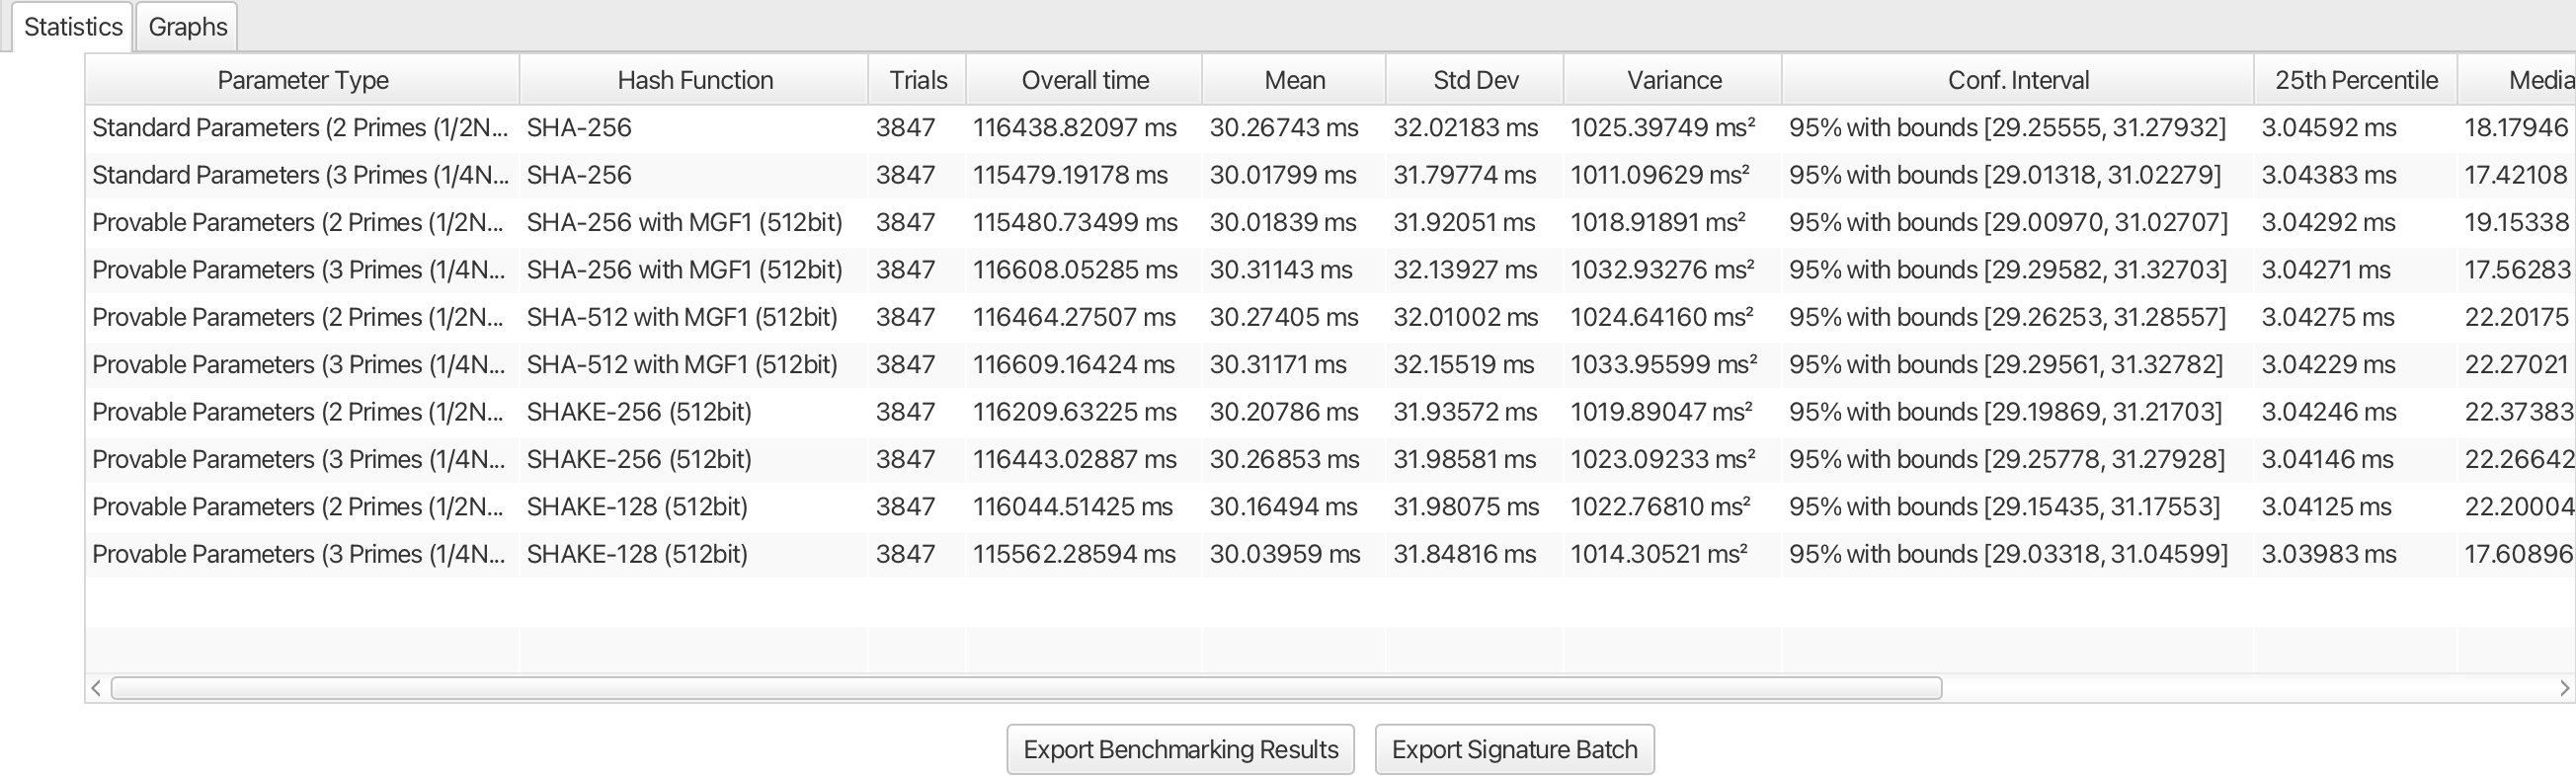
\includegraphics[width=\textwidth]{main_pictures/ansi/ansi_sign_1024bit_table1_1.png}} 
        \fbox{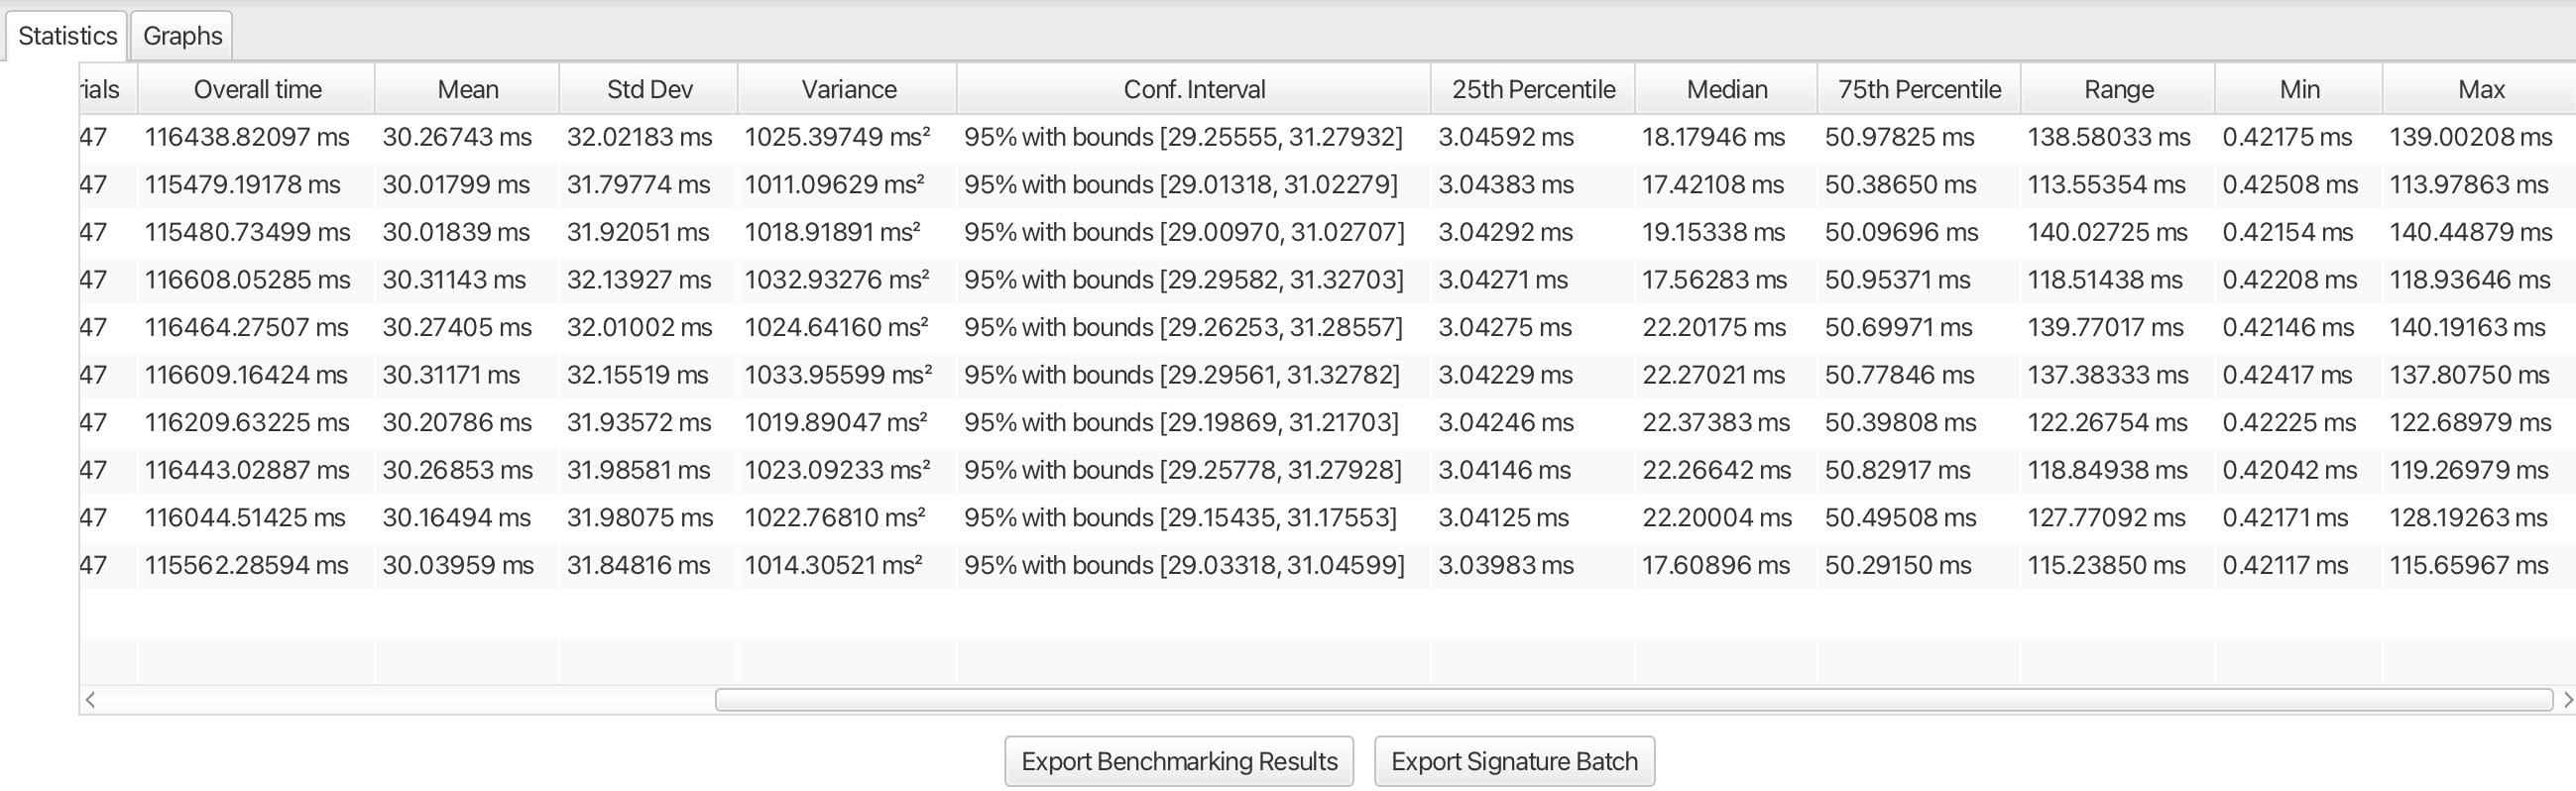
\includegraphics[width=\textwidth]{main_pictures/ansi/ansi_sign_1024bit_table2_1.png}}
    \end{minipage}
            \label{ansi_sign_1024bit_table}
  \end{figure}
  
\begin{figure}[H]
    \centering % Center the images
     \caption{Instantiation of ANSI X9.31 rDSA with standard vs provably secure parameters (2048-bit Key Size) for signature creation}
    % First image in a minipage
    \begin{minipage}{\textwidth}
        \centering
        \fbox{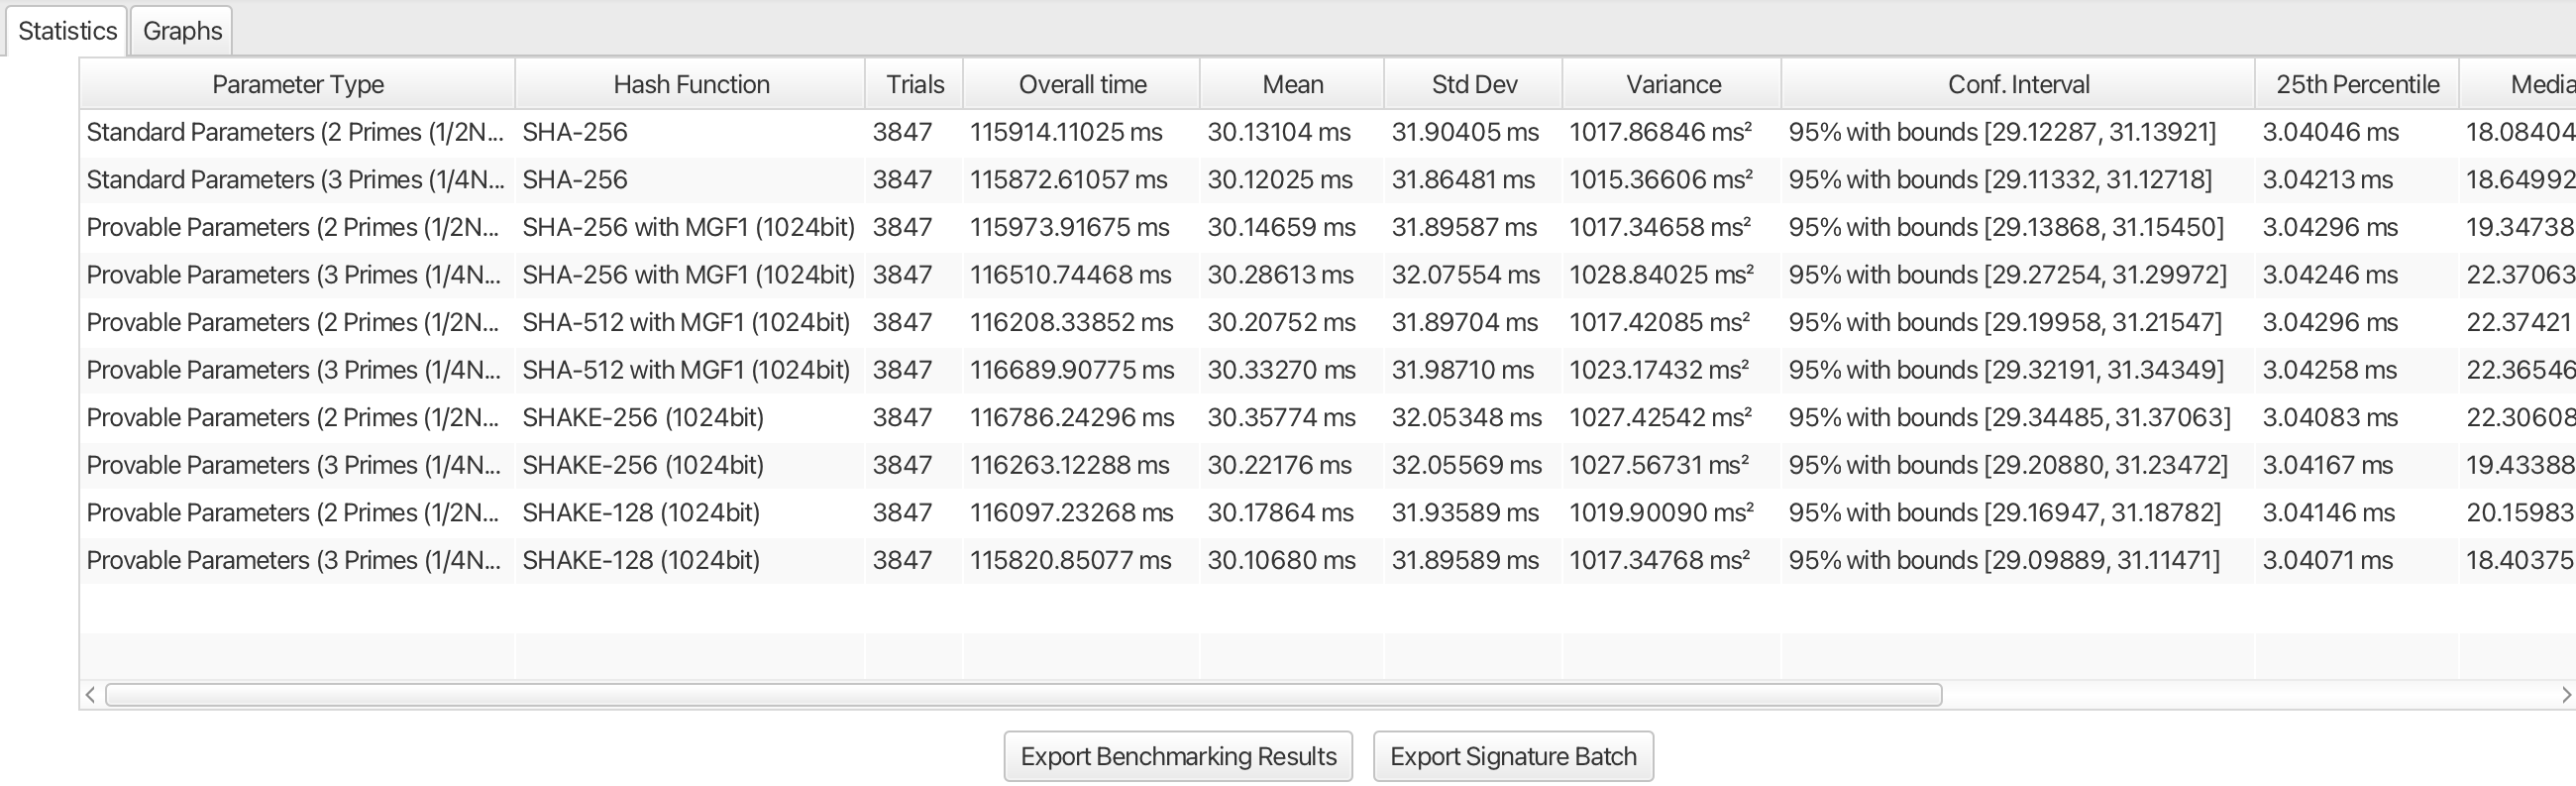
\includegraphics[width=\textwidth]{main_pictures/ansi/ansi_sign_2048bit_table1_1.png}} 
        \fbox{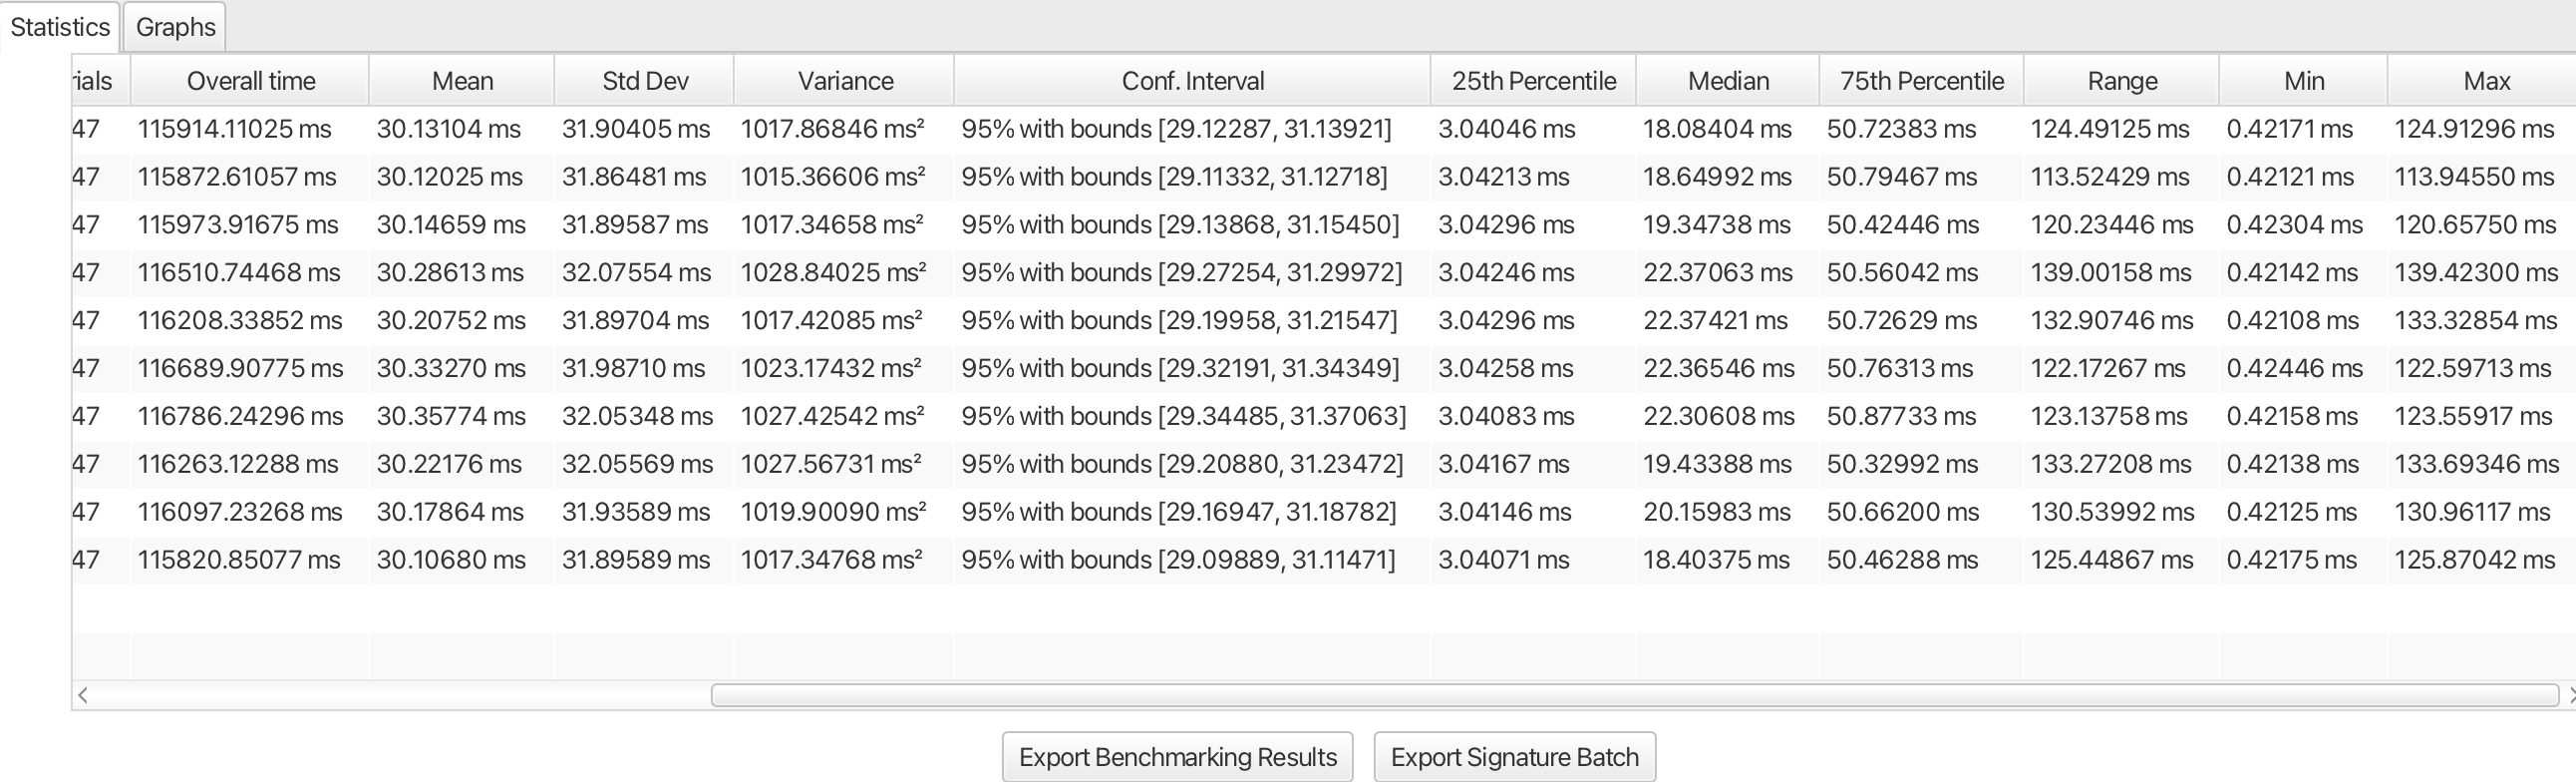
\includegraphics[width=\textwidth]{main_pictures/ansi/ansi_sign_2048bit_table2_1.png}}
    \end{minipage}
            \label{ansi_sign_2048bit_table}
  \end{figure}
  
\begin{figure}[H]
    \centering % Center the images
     \caption{Instantiation of ANSI X9.31 rDSA with standard vs provably secure parameters (3072-bit Key Size) for signature creation}
    % First image in a minipage
    \begin{minipage}{\textwidth}
        \centering
        \fbox{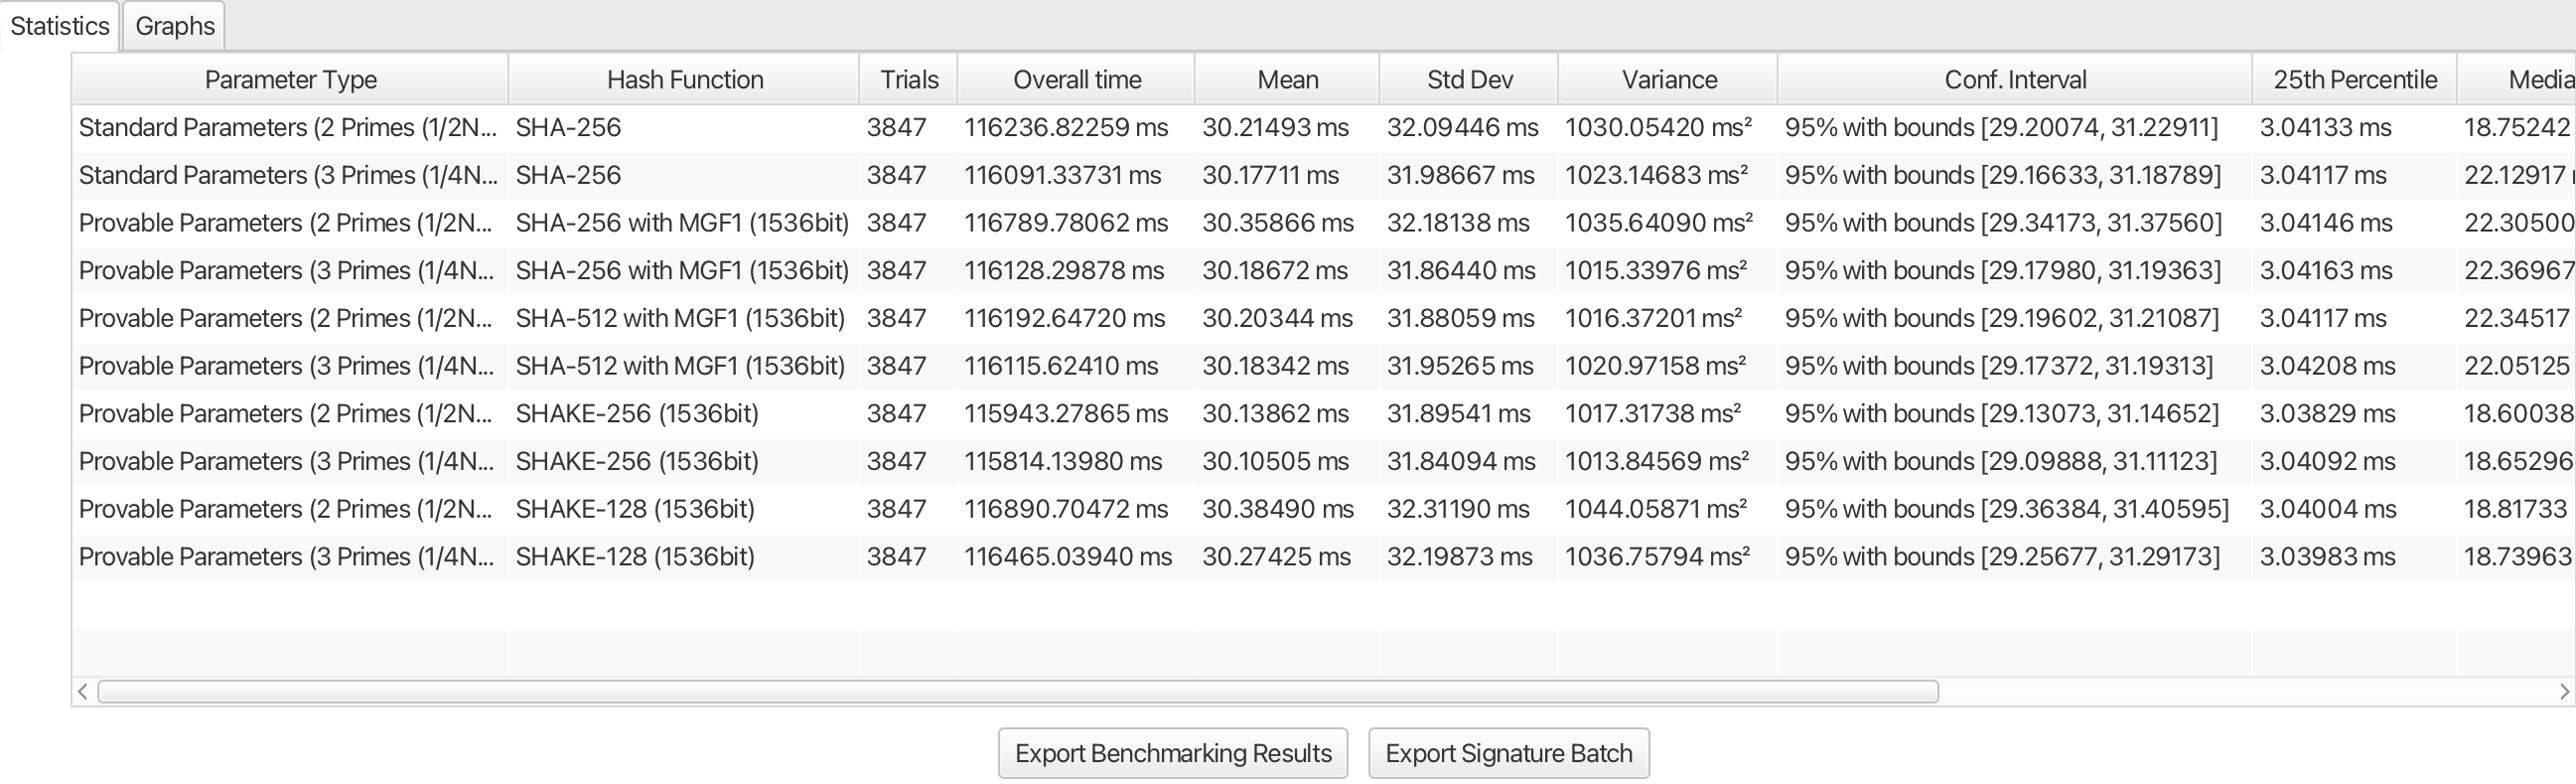
\includegraphics[width=\textwidth]{main_pictures/ansi/ansi_sign_3072bit_table1_1.png}} 
        \fbox{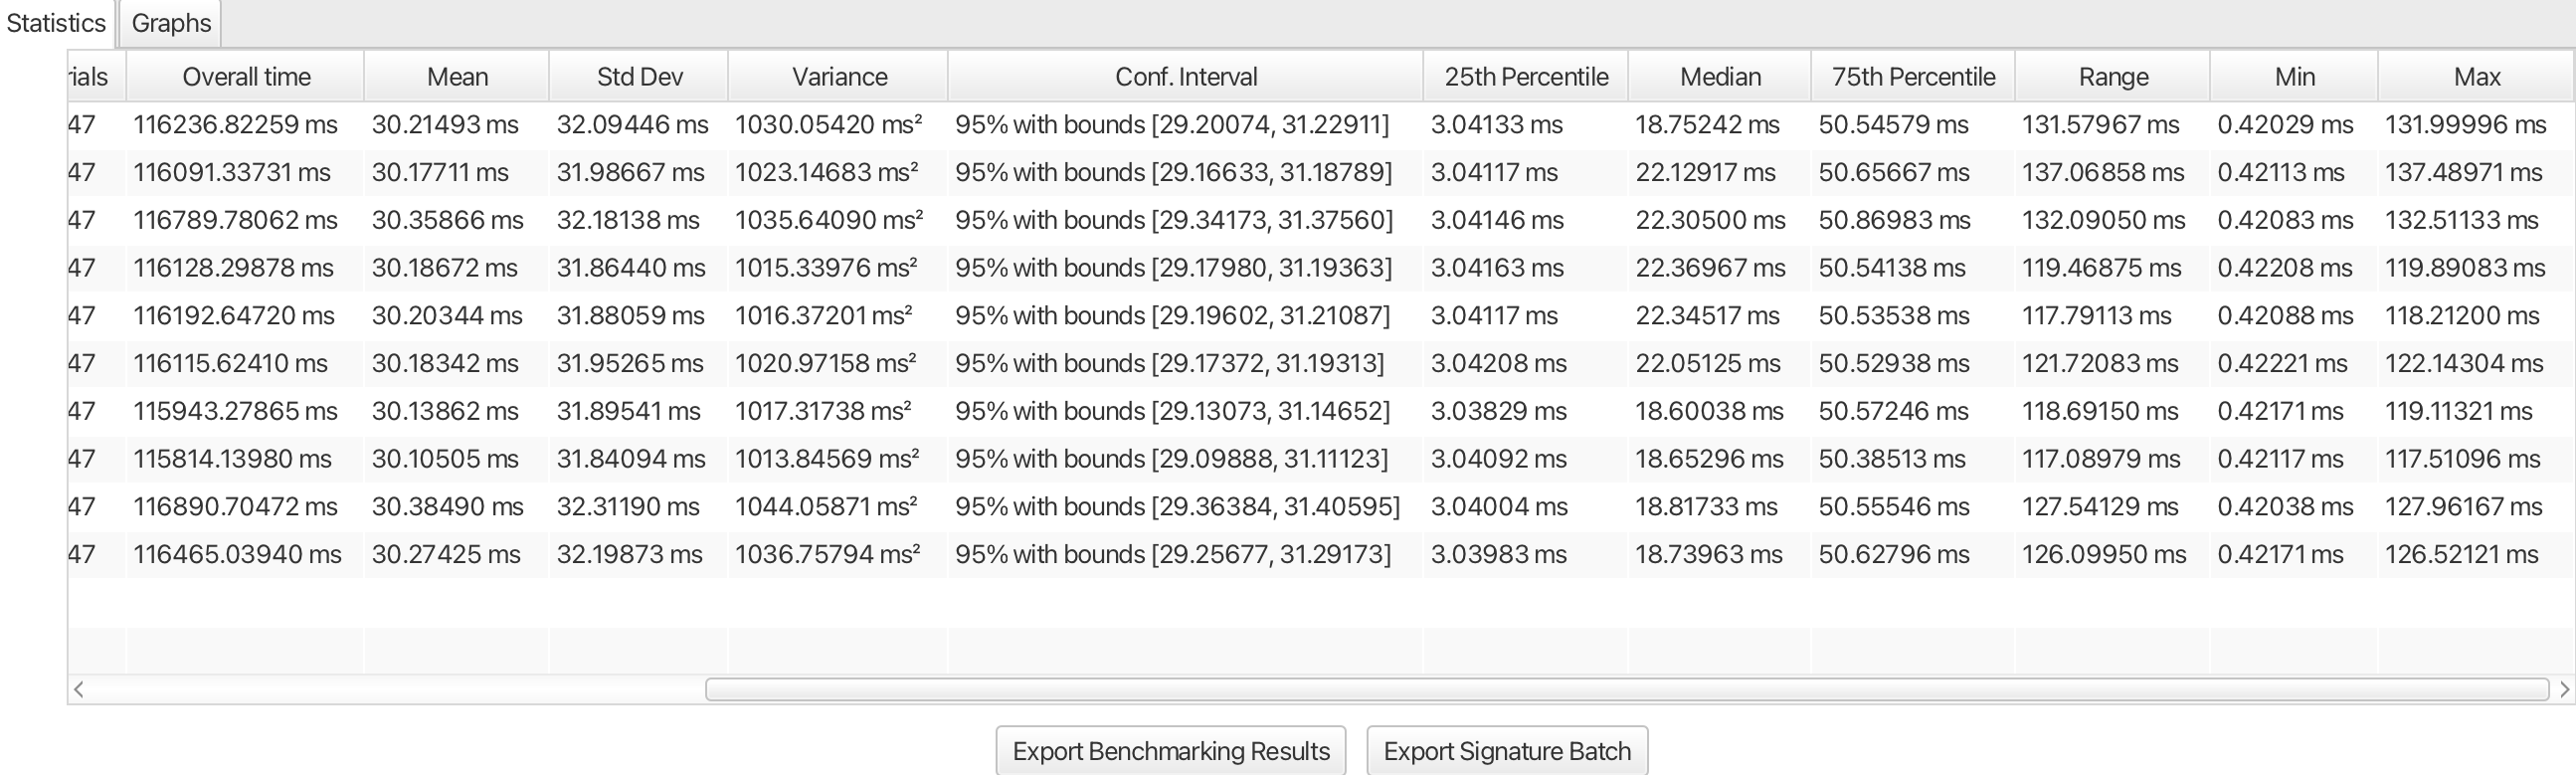
\includegraphics[width=\textwidth]{main_pictures/ansi/ansi_sign_3072bit_table2_1.png}}
    \end{minipage}
         \label{ansi_sign_3072bit_table}
\end{figure}

\begin{figure}[H]
    \centering % Center the images
     \caption{Instantiation of ANSI X9.31 rDSA with standard vs provably secure parameters (4096-bit Key Size) for signature creation}
    % First image in a minipage
    \begin{minipage}{\textwidth}
        \centering
        \fbox{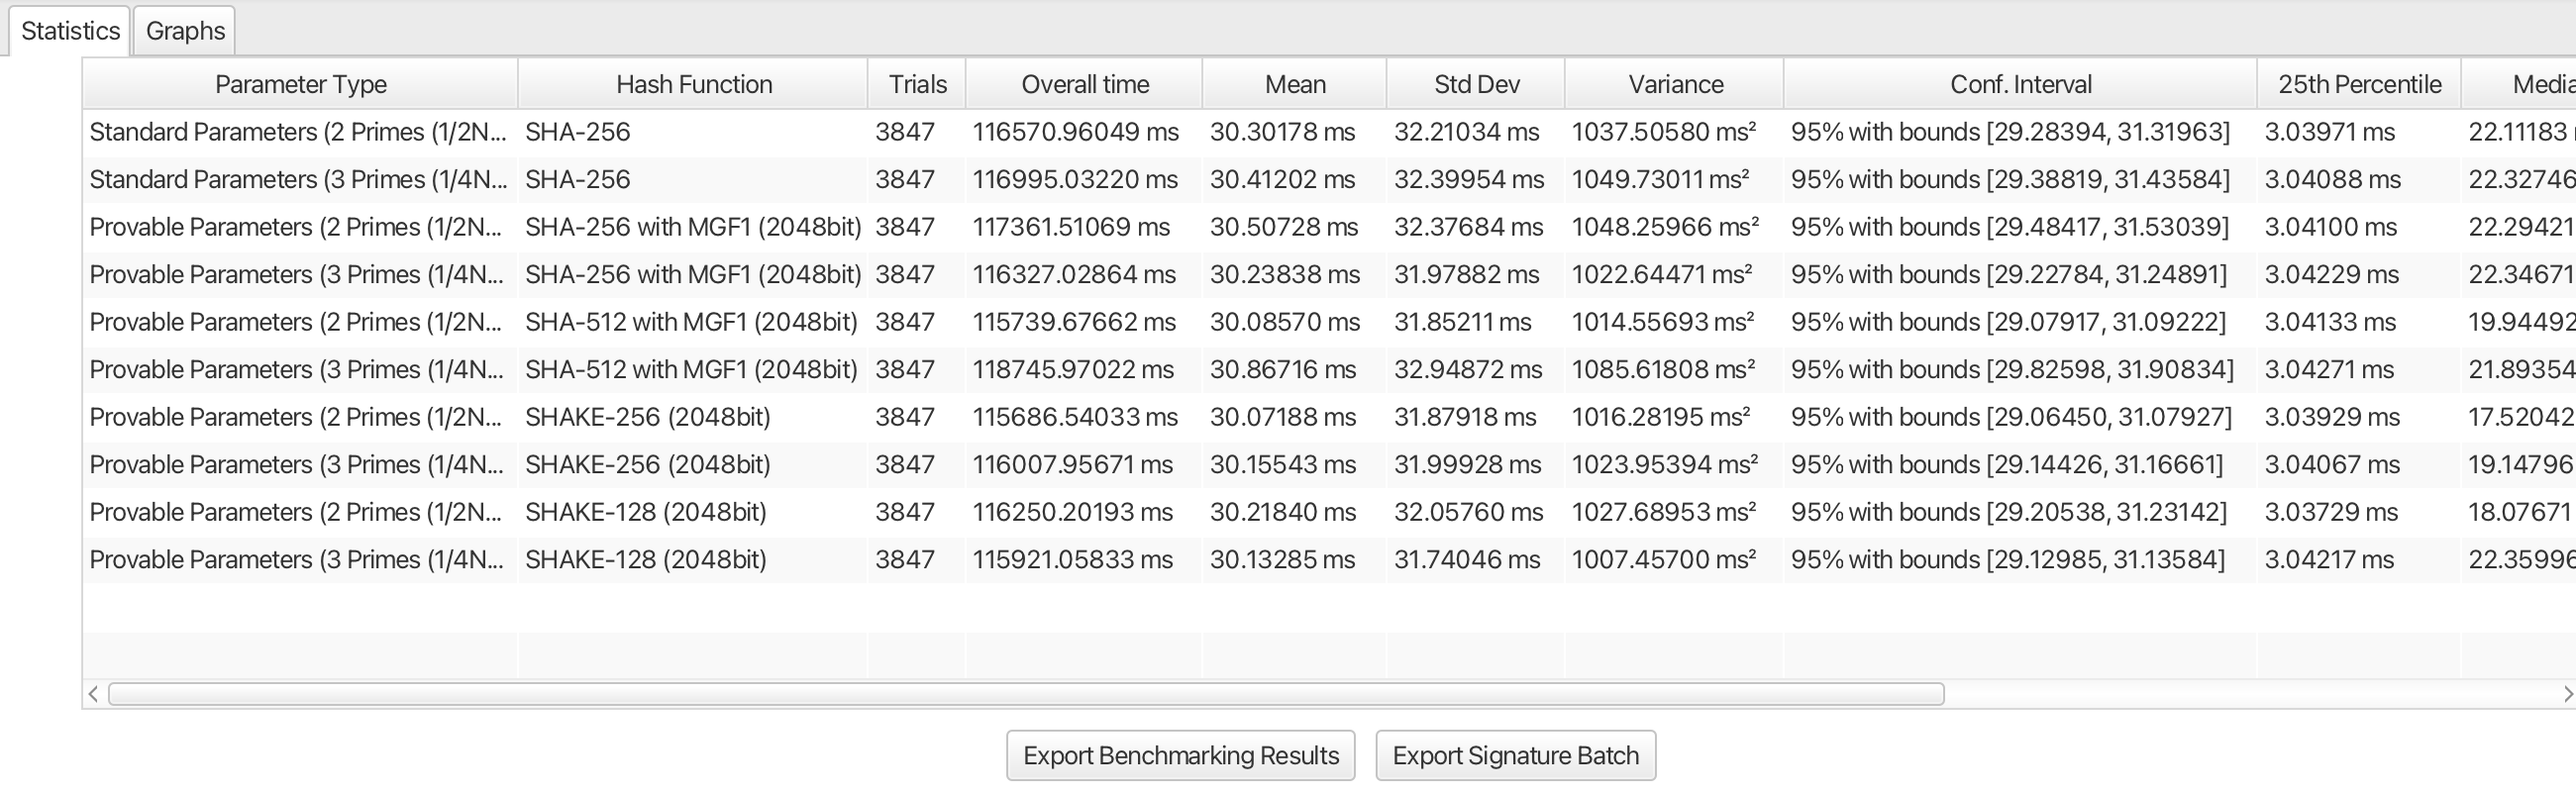
\includegraphics[width=\textwidth]{main_pictures/ansi/ansi_sign_4096bit_table1_1.png}} 
        \fbox{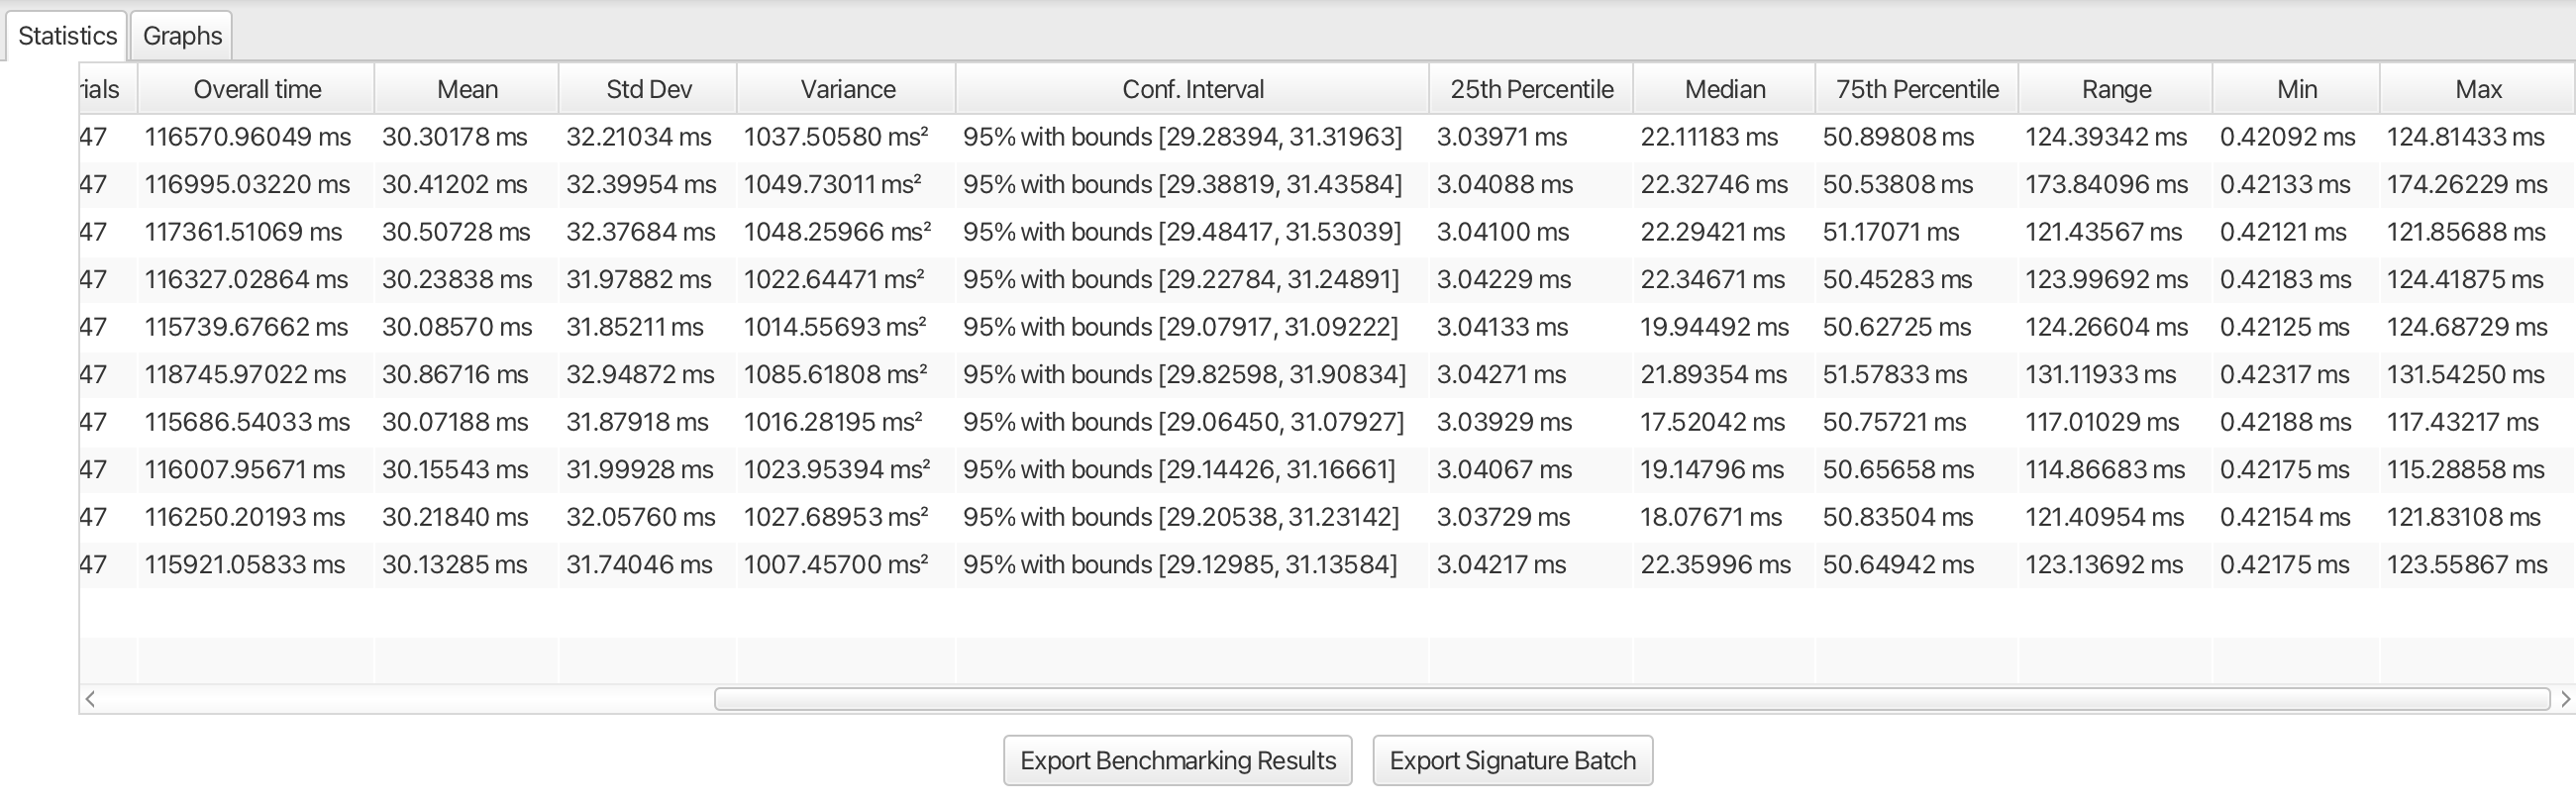
\includegraphics[width=\textwidth]{main_pictures/ansi/ansi_sign_4096bit_table2_1.png}}
    \end{minipage}
             \label{ansi_sign_4096bit_table}
\end{figure}

\begin{figure}[H]
    \centering % Center the images
     \caption{Instantiation of ANSI X9.31 rDSA with standard vs provably secure parameters (5120-bit Key Size) for signature creation}
    % First image in a minipage
    \begin{minipage}{\textwidth}
        \centering
        \fbox{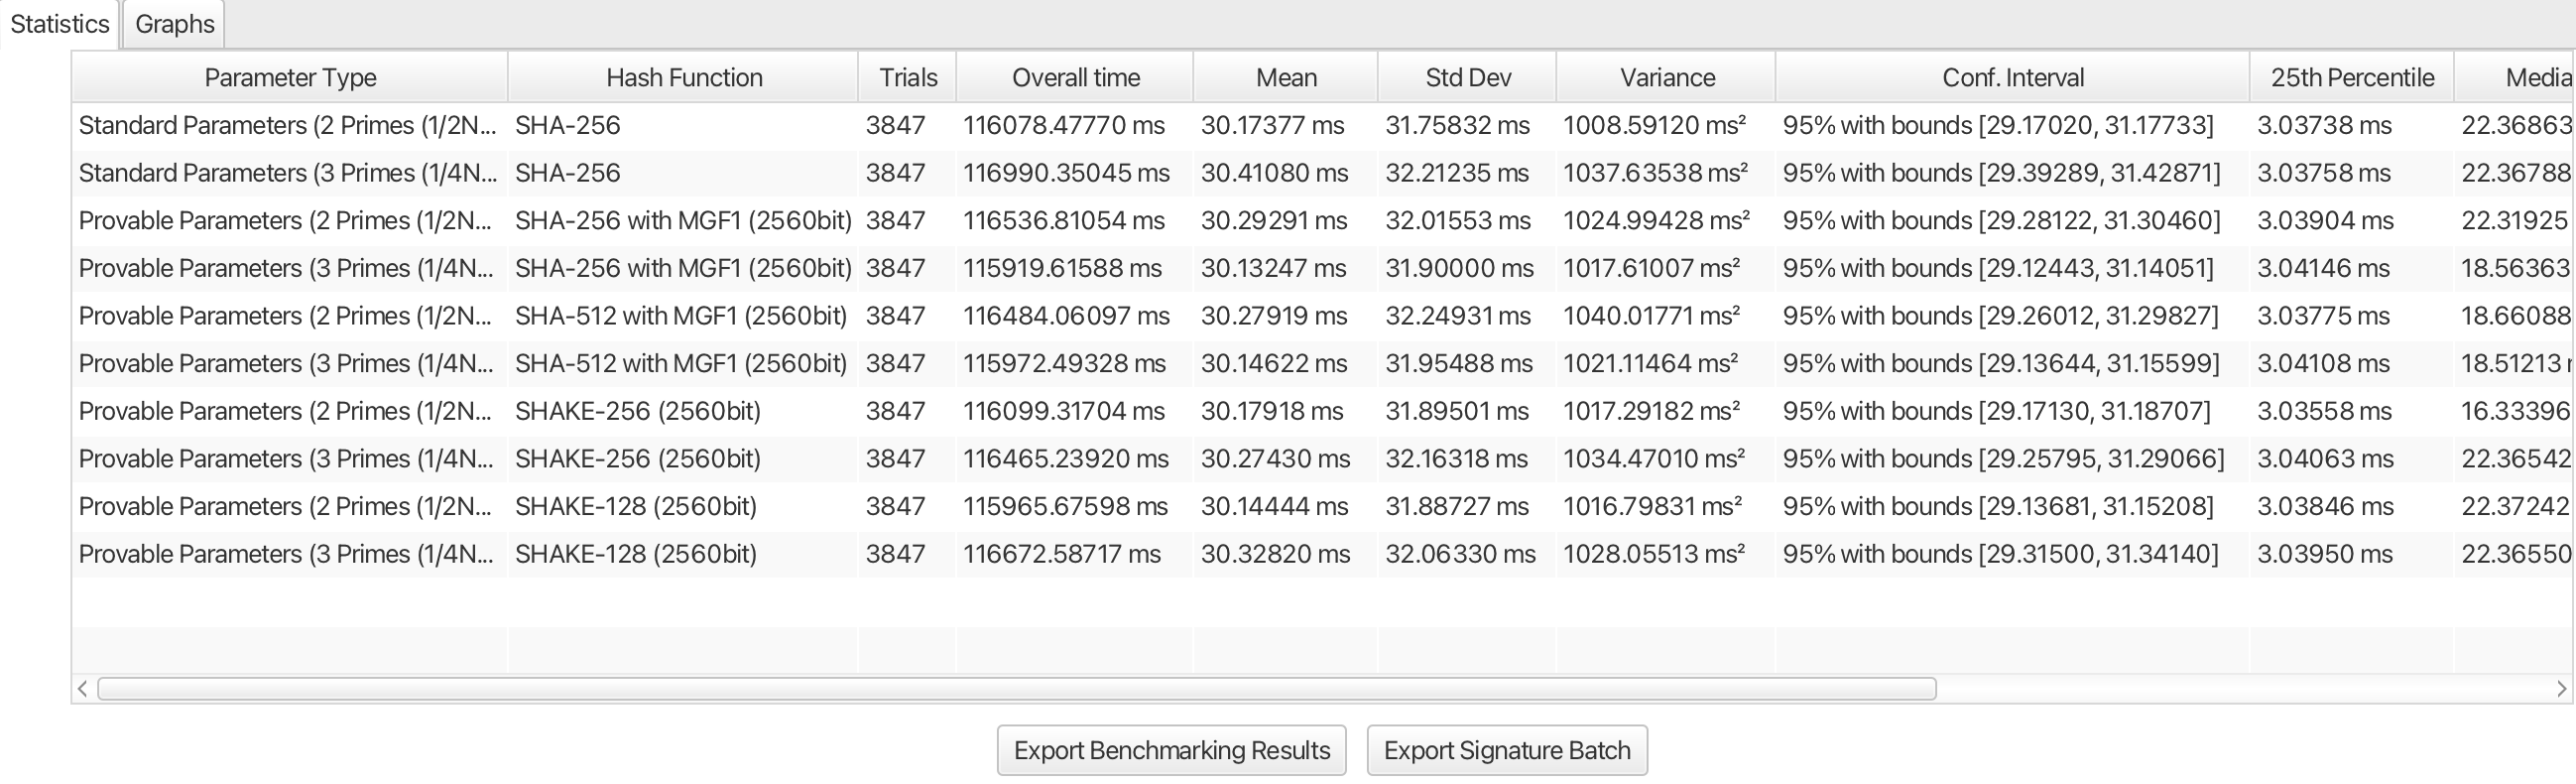
\includegraphics[width=\textwidth]{main_pictures/ansi/ansi_sign_5120bit_table1_1.png}} 
        \fbox{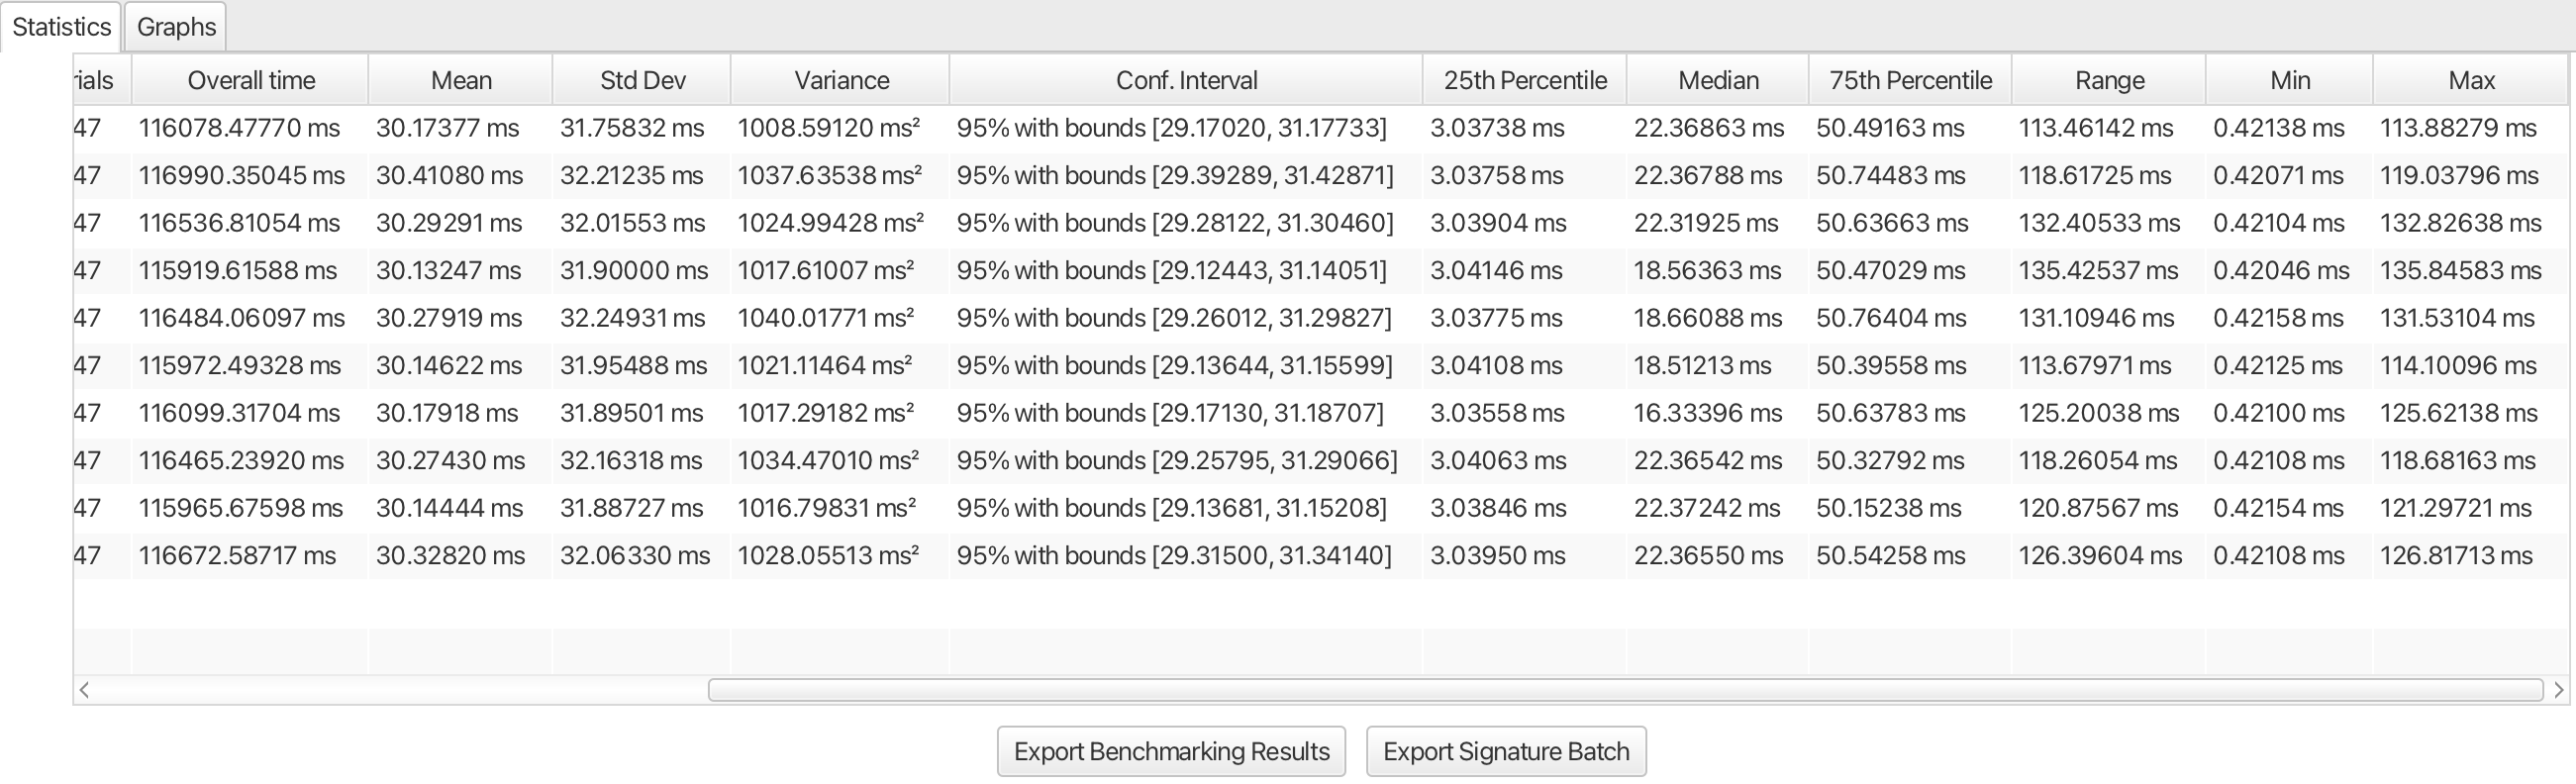
\includegraphics[width=\textwidth]{main_pictures/ansi/ansi_sign_5120bit_table2_1.png}}
    \end{minipage}
     \label{ansi_sign_5120bit_table}
\end{figure}

\begin{figure}[H]
    \centering % Center the images
     \caption{Instantiation of ANSI X9.31 rDSA with standard vs provably secure parameters (6144-bit Key Size) for signature creation}
    % First image in a minipage
    \begin{minipage}{\textwidth}
        \centering
        \fbox{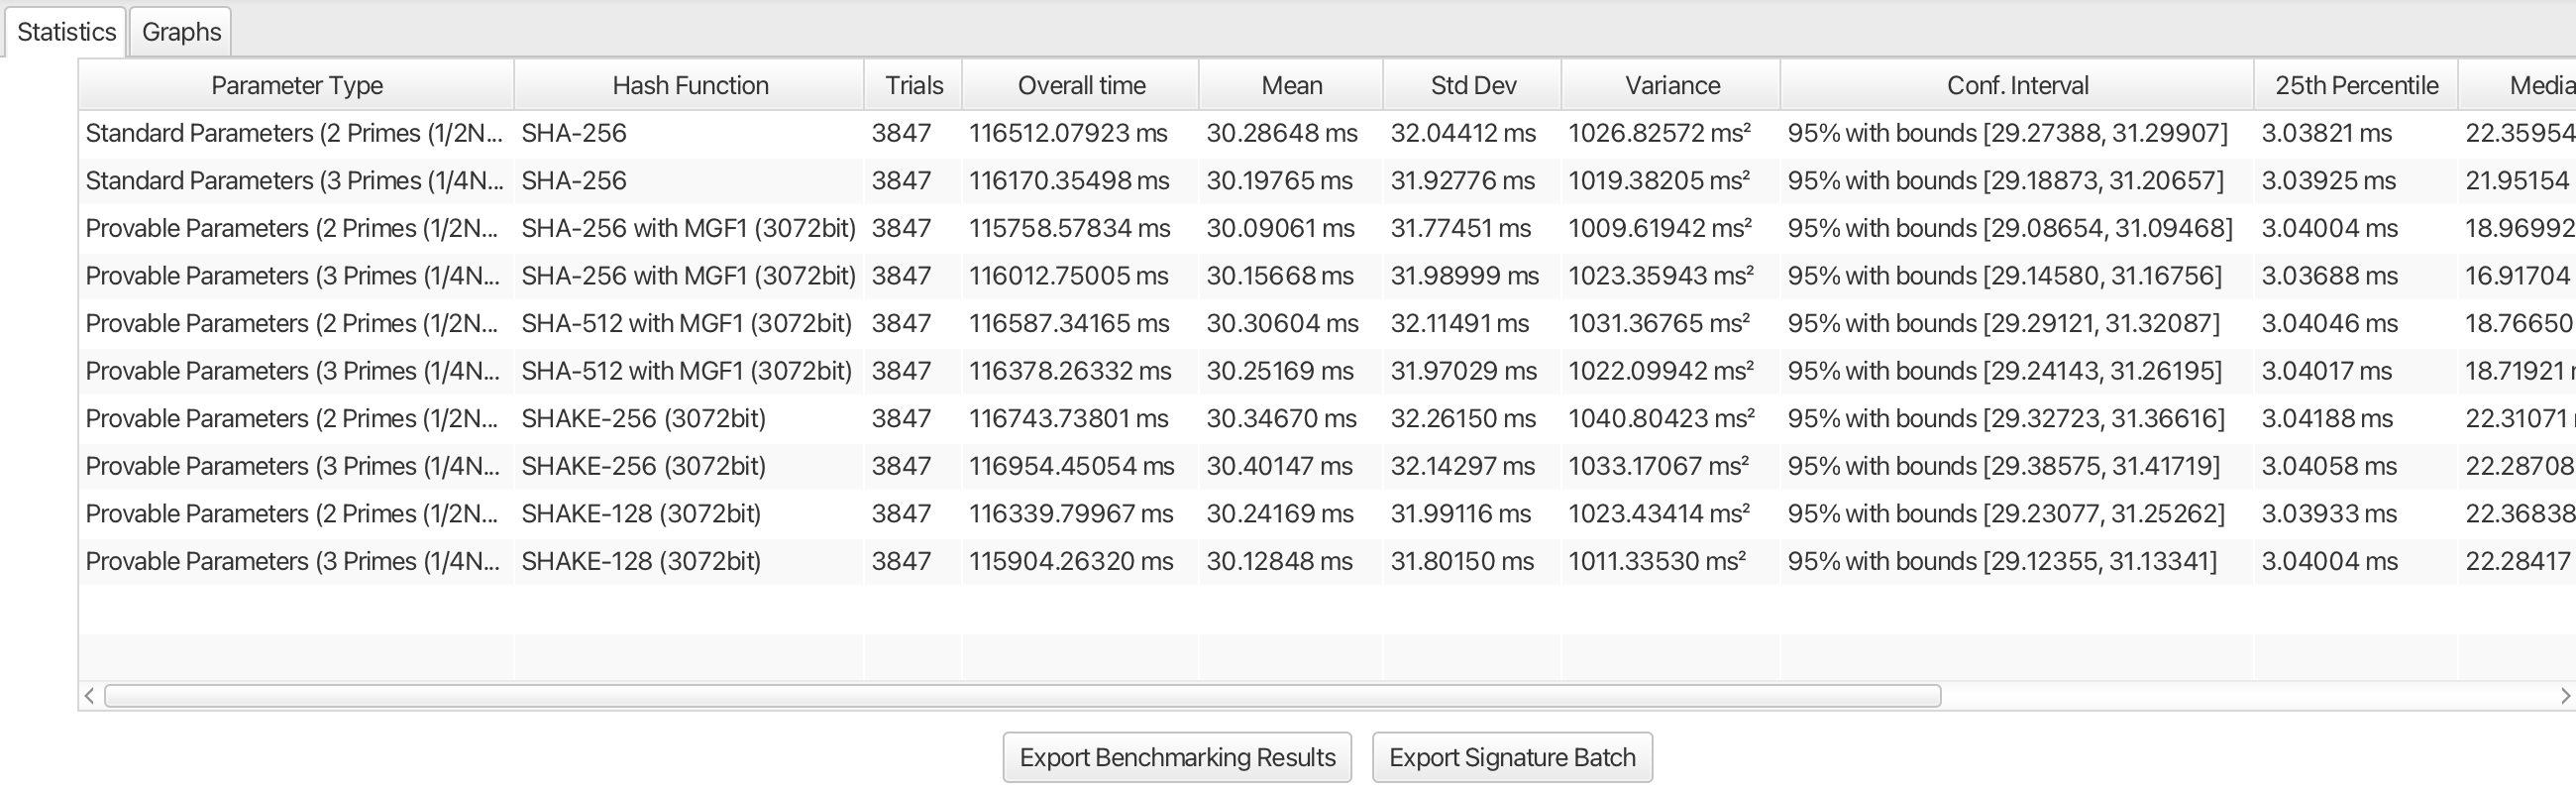
\includegraphics[width=\textwidth]{main_pictures/ansi/ansi_sign_6144bit_table1_1.png}} 
        \fbox{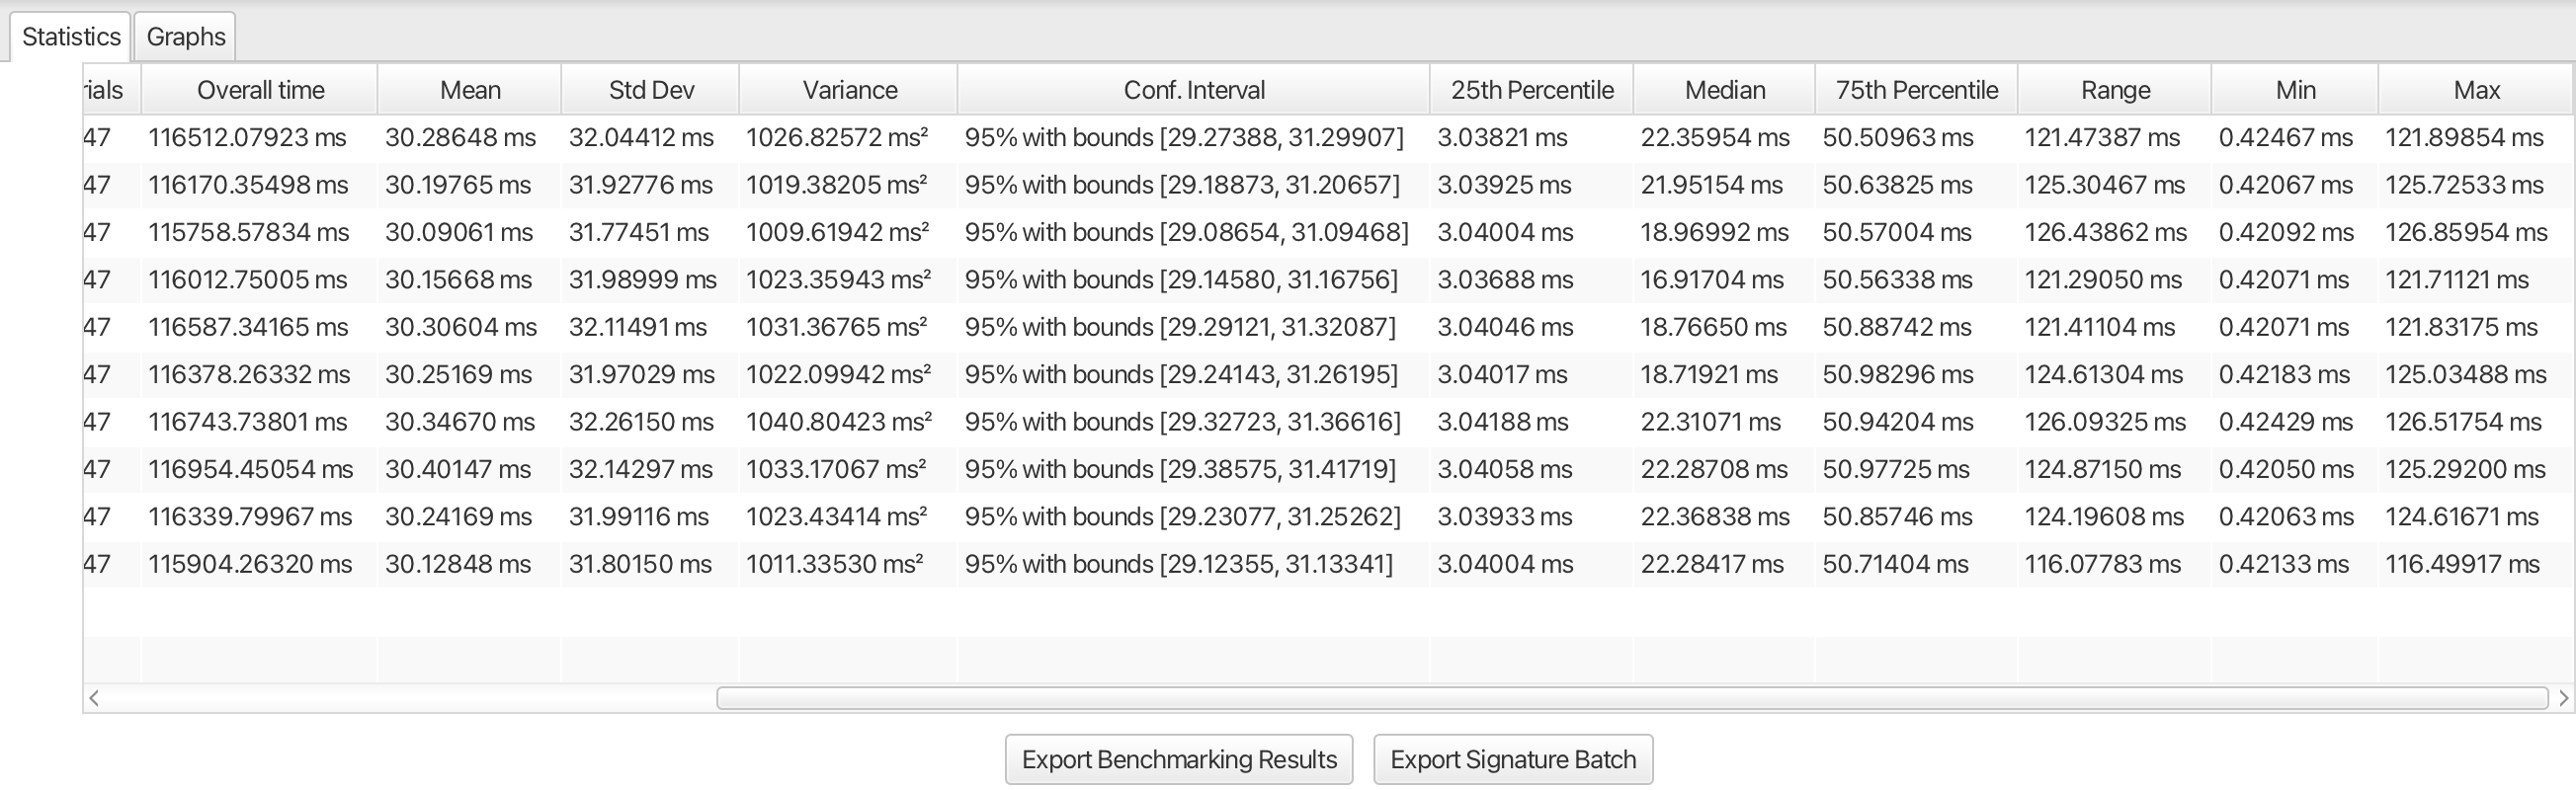
\includegraphics[width=\textwidth]{main_pictures/ansi/ansi_sign_6144bit_table2_1.png}}
    \end{minipage}
         \label{ansi_sign_6144bit_table}
\end{figure}
\end{comment}
\chapter{Appendix C Results Tables for ISO/IEC 9796-2 Scheme 1 and ANSI X9.31 rDSA}


\begin{landscape}
\pagestyle{empty}%


\section{Signature Creation Results (ANSI X9.31 rDSA)}

\begin{longtable}{|p{2.3cm}|p{1.8cm}|p{1.0cm}|p{1.7cm}|p{1.4cm}|p{1.5cm}|p{1.8cm}|p{1.5cm}|p{1.2cm}|p{1.5cm}|p{1.3cm}|p{1.4cm}|p{1.3cm}|p{1.5cm}|}

\caption{\textbf{Instantiation of ANSI X9.31 rDSA with Standard vs Provably Secure Parameters (1024-bit Key Size) for Signature Creation}}
     \label{ansi_sign_1024bit_table} \\
\hline
\textbf{Parameter Type} & \textbf{Hash Function} & \textbf{Trials} & \textbf{Overall Time} & \textbf{Mean} & \textbf{Std Dev} & \textbf{Variance} & \textbf{Conf. Interval} & \textbf{25th Percentile} & \textbf{Median} & \textbf{75th Percentile} & \textbf{Range} & \textbf{Min} & \textbf{Max} \\
\hline
\endfirsthead

\multicolumn{14}{c}%
{{\bfseries \tablename\ \thetable{} -- Signature Creation Results for ANSI X9.31 rDSA with 1024-bit Key Size (continued from previous page)}} \\
\hline
\textbf{Parameter Type} & \textbf{Hash Function} & \textbf{Trials} & \textbf{Overall Time} & \textbf{Mean} & \textbf{Std Dev} & \textbf{Variance} & \textbf{Conf. Interval} & \textbf{25th Percentile} & \textbf{Median} & \textbf{75th Percentile} & \textbf{Range} & \textbf{Min} & \textbf{Max} \\
\hline
\endhead

\hline \multicolumn{14}{|r|}{{Continued on next page}} \\ \hline
\endfoot

\hline
\endlastfoot

Standard Parameters (2 Primes) & SHA-256 & 3847 & 116438.
82097 ms & 30.26743 ms & 32.02183 ms & 1025.39749 ms\textsuperscript{2} & 95\% with bounds 29.25555 ms - 31.27932 ms & 3.04592 ms & 18.17946 ms & 50.97825 ms & 138.58033 ms & 0.42175 ms & 139.00208 ms \\
\hline
Standard Parameters (3 Primes) & SHA-256 & 3847 & 115479.
19178 ms & 30.01799 ms & 31.79774 ms & 1011.09629 ms² & 95\% with bounds 29.01318 ms - 31.02279 ms & 3.04383 ms & 17.42108 ms & 50.38650 ms & 113.55354 ms & 0.42508 ms & 113.97863 ms \\
\hline
Provable Parameters (2 Primes) & SHA-256 with MGF1 (512bit) & 3847 & 115480.
73499 ms & 30.01839 ms & 31.92051 ms & 1018.91891 ms\textsuperscript{2} & 95\% with bounds 29.00970 ms - 31.02707 ms & 3.04292 ms & 19.15338 ms & 50.09696 ms & 140.02725 ms & 0.42154 ms & 140.44879 ms \\
\hline
Provable Parameters (3 Primes) & SHA-256 with MGF1 (512bit) & 3847 & 116608.
05285 ms & 30.31143 ms & 32.13927 ms & 1032.93276 ms\textsuperscript{2} & 95\% with bounds 29.29582 ms - 31.32703 ms & 3.04271 ms & 17.56283 ms & 50.95371 ms & 118.51438 ms & 0.42208 ms & 118.93646 ms \\
\hline
Provable Parameters (2 Primes) & SHA-512 with MGF1 (512bit) & 3847 & 116464.
27507 ms & 30.27405 ms & 32.01002 ms & 1024.64160 ms\textsuperscript{2} & 95\% with bounds 29.26253 ms - 31.28557 ms & 3.04275 ms & 22.20175 ms & 50.69971 ms & 139.77017 ms & 0.42146 ms & 140.19163 ms \\
\hline
Provable Parameters (3 Primes) & SHA-512 with MGF1 (512bit) & 3847 & 116609.
16424 ms & 30.31171 ms & 32.15519 ms & 1033.95599 ms\textsuperscript{2} & 95\% with bounds 29.29561 ms - 31.32782 ms & 3.04229 ms & 22.27021 ms & 50.77846 ms & 137.38333 ms & 0.42417 ms & 137.80750 ms \\
\hline
Provable Parameters (2 Primes) & SHAKE-256 (512bit) & 3847 & 116209.
63225 ms & 30.20786 ms & 31.93572 ms & 1019.89047 ms\textsuperscript{2} & 95\% with bounds 29.19869 ms - 31.21703 ms & 3.04246 ms & 22.37383 ms & 50.39808 ms & 122.26754 ms & 0.42225 ms & 122.68979 ms \\
\hline
Provable Parameters (3 Primes) & SHAKE-256 (512bit) & 3847 & 116443.
02887 ms & 30.26853 ms & 31.98581 ms & 1023.09233 ms\textsuperscript{2} & 95\% with bounds 29.25778 ms - 31.27928 ms & 3.04146 ms & 22.26642 ms & 50.82917 ms & 118.84938 ms & 0.42042 ms & 119.26979 ms \\
\hline
Provable Parameters (2 Primes) & SHAKE-128 (512bit) & 3847 & 116044.
51425 ms & 30.16494 ms & 31.98075 ms & 1022.76810 ms\textsuperscript{2} & 95\% with bounds 29.15435 ms - 31.17553 ms & 3.04125 ms & 22.20004 ms & 50.49508 ms & 127.77092 ms & 0.42171 ms & 128.19263 ms \\
\hline
Provable Parameters (3 Primes) & SHAKE-128 (512bit) & 3847 & 115562.
28594 ms & 30.03959 ms & 31.84816 ms & 1014.30521 ms\textsuperscript{2} & 95\% with bounds 29.03318 ms - 31.04599 ms & 3.03983 ms & 17.60896 ms & 50.29150 ms & 115.23850 ms & 0.42117 ms & 115.65967 ms \\
\hline


\end{longtable}



\begin{longtable}{|p{2.3cm}|p{1.8cm}|p{1.0cm}|p{1.7cm}|p{1.2cm}|p{1.5cm}|p{1.8cm}|p{1.5cm}|p{1.2cm}|p{1.5cm}|p{1.3cm}|p{1.4cm}|p{1.3cm}|p{1.5cm}|}

\caption{\textbf{Instantiation of ANSI X9.31 rDSA with Standard vs Provably Secure Parameters (2048-bit Key Size) for Signature Creation}}
     \label{ansi_sign_2048bit_table} \\
\hline
\textbf{Parameter Type} & \textbf{Hash Function} & \textbf{Trials} & \textbf{Overall Time} & \textbf{Mean} & \textbf{Std Dev} & \textbf{Variance} & \textbf{Conf. Interval} & \textbf{25th Percentile} & \textbf{Median} & \textbf{75th Percentile} & \textbf{Range} & \textbf{Min} & \textbf{Max} \\
\hline
\endfirsthead

\multicolumn{14}{c}%
{{\bfseries \tablename\ \thetable{} -- Signature Creation Results for ANSI X9.31 rDSA with 2048-bit Key Size (continued from previous page)}} \\
\hline
\textbf{Parameter Type} & \textbf{Hash Function} & \textbf{Trials} & \textbf{Overall Time} & \textbf{Mean} & \textbf{Std Dev} & \textbf{Variance} & \textbf{Conf. Interval} & \textbf{25th Percentile} & \textbf{Median} & \textbf{75th Percentile} & \textbf{Range} & \textbf{Min} & \textbf{Max} \\
\hline
\endhead

\hline \multicolumn{14}{|r|}{{Continued on next page}} \\ \hline
\endfoot

\hline
\endlastfoot

Standard Parameters (2 Primes) & SHA-256 & 3847 & 115914.
11025 ms & 30.13104 ms & 31.90405 ms & 1017.86846 ms\textsuperscript{2} & 95\% with bounds 29.12287 ms - 31.13921 ms & 3.04046 ms & 18.08404 ms & 50.72383 ms & 124.49125 ms & 0.42171 ms & 124.91296 ms \\
\hline
Standard Parameters (3 Primes) & SHA-256 & 3847 & 115872.
61057 ms & 30.12025 ms & 31.86481 ms & 1015.36606 ms\textsuperscript{2} & 95\% with bounds 29.11332 ms - 31.12718 ms & 3.04213 ms & 18.64992 ms & 50.79467 ms & 113.52429 ms & 0.42121 ms & 113.94550 ms \\
\hline
Provable Parameters (2 Primes) & SHA-256 with MGF1 (1024bit) & 3847 & 115973.
91675 ms & 30.14659 ms & 31.89587 ms & 1017.34658 ms\textsuperscript{2} & 95\% with bounds 29.13868 ms - 31.15450 ms & 3.04296 ms & 19.34738 ms & 50.42446 ms & 120.23446 ms & 0.42304 ms & 120.65750 ms \\
\hline
Provable Parameters (3 Primes) & SHA-256 with MGF1 (1024bit) & 3847 & 116510.
74468 ms & 30.28613 ms & 32.07554 ms & 1028.84025 ms\textsuperscript{2} & 95\% with bounds 29.27254 ms - 31.29972 ms & 3.04246 ms & 22.37063 ms & 50.56042 ms & 139.00158 ms & 0.42142 ms & 139.42300 ms \\
\hline
Provable Parameters (2 Primes) & SHA-512 with MGF1 (1024bit) & 3847 & 116208.
33852 ms & 30.20752 ms & 31.89704 ms & 1017.42085 ms\textsuperscript{2} & 95\% with bounds 29.19958 ms - 31.21547 ms & 3.04296 ms & 22.37421 ms & 50.72629 ms & 132.90746 ms & 0.42108 ms & 133.32854 ms \\
\hline
Provable Parameters (3 Primes) & SHA-512 with MGF1 (1024bit) & 3847 & 116689.
90775 ms & 30.33270 ms & 31.98710 ms & 1023.17432 ms\textsuperscript{2} & 95\% with bounds 29.32191 ms - 31.34349 ms & 3.04258 ms & 22.36546 ms & 50.76313 ms & 122.17267 ms & 0.42446 ms & 122.59713 ms \\
\hline
Provable Parameters (2 Primes) & SHAKE-256 (1024bit) & 3847 & 116786.
24296 ms & 30.35774 ms & 32.05348 ms & 1027.42542 ms\textsuperscript{2} & 95\% with bounds 29.34485 ms - 31.37063 ms & 3.04083 ms & 22.30608 ms & 50.87733 ms & 123.13758 ms & 0.42158 ms & 123.55917 ms \\
\hline
Provable Parameters (3 Primes) & SHAKE-256 (1024bit) & 3847 & 116263.
12288 ms & 30.22176 ms & 32.05569 ms & 1027.56731 ms\textsuperscript{2} & 95\% with bounds 29.20880 ms - 31.23472 ms & 3.04167 ms & 19.43388 ms & 50.32992 ms & 133.27208 ms & 0.42138 ms & 133.69346 ms \\
\hline
Provable Parameters (2 Primes) & SHAKE-128 (1024bit) & 3847 & 116097.
23268 ms & 30.17864 ms & 31.93589 ms & 1019.90090 ms\textsuperscript{2} & 95\% with bounds 29.16947 ms - 31.18782 ms & 3.04146 ms & 20.15983 ms & 50.66200 ms & 130.53992 ms & 0.42125 ms & 130.96117 ms \\
\hline
Provable Parameters (3 Primes) & SHAKE-128 (1024bit) & 3847 & 115820.
85077 ms & 30.10680 ms & 31.89589 ms & 1017.34768 ms\textsuperscript{2} & 95\% with bounds 29.09889 ms - 31.11471 ms & 3.04071 ms & 18.40375 ms & 50.46288 ms & 125.44867 ms & 0.42175 ms & 125.87042 ms \\
\hline



\end{longtable}

\begin{longtable}{|p{2.3cm}|p{1.8cm}|p{1.0cm}|p{1.7cm}|p{1.2cm}|p{1.5cm}|p{1.8cm}|p{1.5cm}|p{1.2cm}|p{1.5cm}|p{1.3cm}|p{1.4cm}|p{1.3cm}|p{1.5cm}|}

\caption{\textbf{Instantiation of ANSI X9.31 rDSA with Standard vs Provably Secure Parameters (3072-bit Key Size) for Signature Creation}}
     \label{ansi_sign_3072bit_table} \\
\hline
\textbf{Parameter Type} & \textbf{Hash Function} & \textbf{Trials} & \textbf{Overall Time} & \textbf{Mean} & \textbf{Std Dev} & \textbf{Variance} & \textbf{Conf. Interval} & \textbf{25th Percentile} & \textbf{Median} & \textbf{75th Percentile} & \textbf{Range} & \textbf{Min} & \textbf{Max} \\
\hline
\endfirsthead

\multicolumn{14}{c}%
{{\bfseries \tablename\ \thetable{} -- Signature Creation Results for ANSI X9.31 rDSA with 3072-bit Key Size (continued from previous page)}} \\
\hline
\textbf{Parameter Type} & \textbf{Hash Function} & \textbf{Trials} & \textbf{Overall Time} & \textbf{Mean} & \textbf{Std Dev} & \textbf{Variance} & \textbf{Conf. Interval} & \textbf{25th Percentile} & \textbf{Median} & \textbf{75th Percentile} & \textbf{Range} & \textbf{Min} & \textbf{Max} \\
\hline
\endhead

\hline \multicolumn{14}{|r|}{{Continued on next page}} \\ \hline
\endfoot

\hline
\endlastfoot

Standard Parameters (2 Primes) & SHA-256 & 3847 & 116236.
82259 ms & 30.21493 ms & 32.09446 ms & 1030.05420 ms\textsuperscript{2}& 95\% with bounds 29.20074 ms - 31.22911 ms & 3.04133 ms & 18.75242 ms & 50.54579 ms & 131.57967 ms & 0.42029 ms & 131.99996 ms \\
\hline
Standard Parameters (3 Primes) & SHA-256 & 3847 & 116091.
33731 ms & 30.17711 ms & 31.98667 ms & 1023.14683 ms\textsuperscript{2} & 95\% with bounds 29.16633 ms - 31.18789 ms & 3.04117 ms & 22.12917 ms & 50.65667 ms & 137.06858 ms & 0.42113 ms & 137.48971 ms \\
\hline
Provable Parameters (2 Primes) & SHA-256 with MGF1 (1536bit) & 3847 & 116789.
78062 ms & 30.35866 ms & 32.18138 ms & 1035.64090 ms\textsuperscript{2} & 95\% with bounds 29.34173 ms - 31.37560 ms & 3.04146 ms & 22.30500 ms & 50.86983 ms & 132.09050 ms & 0.42083 ms & 132.51133 ms \\
\hline
Provable Parameters (3 Primes) & SHA-256 with MGF1 (1536bit) & 3847 & 116128.
29878 ms & 30.18672 ms & 31.86440 ms & 1015.33976 ms\textsuperscript{2} & 95\% with bounds 29.17980 ms - 31.19363 ms & 3.04163 ms & 22.36967 ms & 50.54138 ms & 119.46875 ms & 0.42208 ms & 119.89083 ms \\
\hline
Provable Parameters (2 Primes) & SHA-512 with MGF1 (1536bit) & 3847 & 116192.
64720 ms & 30.20344 ms & 31.88059 ms & 1016.37201 ms² & 95\% with bounds 29.19602 ms - 31.21087 ms & 3.04117 ms & 22.34517 ms & 50.53538 ms & 117.79113 ms & 0.42088 ms & 118.21200 ms \\
\hline
Provable Parameters (3 Primes) & SHA-512 with MGF1 (1536bit) & 3847 & 116115.
62410 ms & 30.18342 ms & 31.95265 ms & 1020.97158 ms\textsuperscript{2} & 95\% with bounds 29.17372 ms - 31.19313 ms & 3.04208 ms & 22.05125 ms & 50.52938 ms & 121.72083 ms & 0.42221 ms & 122.14304 ms \\
\hline
Provable Parameters (2 Primes) & SHAKE-256 (1536bit) & 3847 & 115943.
27865 ms & 30.13862 ms & 31.89541 ms & 1017.31738 ms\textsuperscript{2} & 95\% with bounds 29.13073 ms - 31.14652 ms & 3.03829 ms & 18.60038 ms & 50.57246 ms & 118.69150 ms & 0.42171 ms & 119.11321 ms \\
\hline
Provable Parameters (3 Primes) & SHAKE-256 (1536bit) & 3847 & 115814.
13980 ms & 30.10505 ms & 31.84094 ms & 1013.84569 ms\textsuperscript{2}& 95\% with bounds 29.09888 ms - 31.11123 ms & 3.04092 ms & 18.65296 ms & 50.38513 ms & 117.08979 ms & 0.42117 ms & 117.51096 ms \\
\hline
Provable Parameters (2 Primes) & SHAKE-128 (1536bit) & 3847 & 116890.
70472 ms & 30.38490 ms & 32.31190 ms & 1044.05871 ms\textsuperscript{2} & 95\% with bounds 29.36384 ms - 31.40595 ms & 3.04004 ms & 18.81733 ms & 50.55546 ms & 127.54129 ms & 0.42038 ms & 127.96167 ms \\
\hline
Provable Parameters (3 Primes) & SHAKE-128 (1536bit) & 3847 & 116465.
03940 ms & 30.27425 ms & 32.19873 ms & 1036.75794 ms\textsuperscript{2} & 95\% with bounds 29.25677 ms - 31.29173 ms & 3.03983 ms & 18.73963 ms & 50.62796 ms & 126.09950 ms & 0.42171 ms & 126.52121 ms \\
\hline



\end{longtable}



\begin{longtable}{|p{2.3cm}|p{1.8cm}|p{1.0cm}|p{1.7cm}|p{1.2cm}|p{1.5cm}|p{1.8cm}|p{1.5cm}|p{1.2cm}|p{1.5cm}|p{1.3cm}|p{1.4cm}|p{1.3cm}|p{1.5cm}|}

\caption{\textbf{Instantiation of ANSI X9.31 rDSA with Standard vs Provably Secure Parameters (4096-bit Key Size) for Signature Creation}}
     \label{ansi_sign_4096bit_table} \\
\hline
\textbf{Parameter Type} & \textbf{Hash Function} & \textbf{Trials} & \textbf{Overall Time} & \textbf{Mean} & \textbf{Std Dev} & \textbf{Variance} & \textbf{Conf. Interval} & \textbf{25th Percentile} & \textbf{Median} & \textbf{75th Percentile} & \textbf{Range} & \textbf{Min} & \textbf{Max} \\
\hline
\endfirsthead

\multicolumn{14}{c}%
{{\bfseries \tablename\ \thetable{} -- Signature Creation Results for ANSI X9.31 rDSA with 4096-bit Key Size (continued from previous page)}} \\
\hline
\textbf{Parameter Type} & \textbf{Hash Function} & \textbf{Trials} & \textbf{Overall Time} & \textbf{Mean} & \textbf{Std Dev} & \textbf{Variance} & \textbf{Conf. Interval} & \textbf{25th Percentile} & \textbf{Median} & \textbf{75th Percentile} & \textbf{Range} & \textbf{Min} & \textbf{Max} \\
\hline
\endhead

\hline \multicolumn{14}{|r|}{{Continued on next page}} \\ \hline
\endfoot

\hline
\endlastfoot

Standard Parameters (2 Primes) & SHA-256 & 3847 & 116570.
96049 ms & 30.30178 ms & 32.21034 ms & 1037.50580 ms\textsuperscript{2} & 95\% with bounds 29.28394 ms - 31.31963 ms & 3.03971 ms & 22.11183 ms & 50.89808 ms & 124.39342 ms & 0.42092 ms & 124.81433 ms \\
\hline
Standard Parameters (3 Primes) & SHA-256 & 3847 & 116995.
03220 ms & 30.41202 ms & 32.39954 ms & 1049.73011 ms\textsuperscript{2} & 95\% with bounds 29.38819 ms - 31.43584 ms & 3.04088 ms & 22.32746 ms & 50.53808 ms & 173.84096 ms & 0.42133 ms & 174.26229 ms \\
\hline
Provable Parameters (2 Primes) & SHA-256 with MGF1 (2048bit) & 3847 & 117361.
51069 ms & 30.50728 ms & 32.37684 ms & 1048.25966 ms\textsuperscript{2} & 95\% with bounds 29.48417 ms - 31.53039 ms & 3.04100 ms & 22.29421 ms & 51.17071 ms & 121.43567 ms & 0.42121 ms & 121.85688 ms \\
\hline
Provable Parameters (3 Primes) & SHA-256 with MGF1 (2048bit) & 3847 & 116327.
02864 ms & 30.23838 ms & 31.97882 ms & 1022.64471 ms\textsuperscript{2} & 95\% with bounds 29.22784 ms - 31.24891 ms & 3.04229 ms & 22.34671 ms & 50.45283 ms & 123.99692 ms & 0.42183 ms & 124.41875 ms \\
\hline
Provable Parameters (2 Primes) & SHA-512 with MGF1 (2048bit) & 3847 & 115739.
67662 ms & 30.08570 ms & 31.85211 ms & 1014.55693 ms\textsuperscript{2} & 95\% with bounds 29.07917 ms - 31.09222 ms & 3.04133 ms & 19.94492 ms & 50.62725 ms & 124.26604 ms & 0.42125 ms & 124.68729 ms \\
\hline
Provable Parameters (3 Primes) & SHA-512 with MGF1 (2048bit) & 3847 & 118745.
97022 ms & 30.86716 ms & 32.94872 ms & 1085.61808 ms\textsuperscript{2} & 95\% with bounds 29.82598 ms - 31.90834 ms & 3.04271 ms & 21.89354 ms & 51.57833 ms & 131.11933 ms & 0.42317 ms & 131.54250 ms \\
\hline
Provable Parameters (2 Primes) & SHAKE-256 (2048bit) & 3847 & 115686.
54033 ms & 30.07188 ms & 31.87918 ms & 1016.28195 ms\textsuperscript{2} & 95\% with bounds 29.06450 ms - 31.07927 ms & 3.03929 ms & 17.52042 ms & 50.75721 ms & 117.01029 ms & 0.42188 ms & 117.43217 ms \\
\hline
Provable Parameters (3 Primes) & SHAKE-256 (2048bit) & 3847 & 116007.
95671 ms & 30.15543 ms & 31.99928 ms & 1023.95394 ms\textsuperscript{2} & 95\% with bounds 29.14426 ms - 31.16661 ms & 3.04067 ms & 19.14796 ms & 50.65658 ms & 114.86683 ms & 0.42175 ms & 115.28858 ms \\
\hline
Provable Parameters (2 Primes) & SHAKE-128 (2048bit) & 3847 & 116250.
20193 ms & 30.21840 ms & 32.05760 ms & 1027.68953 ms\textsuperscript{2} & 95\% with bounds 29.20538 ms - 31.23142 ms & 3.03729 ms & 18.07671 ms & 50.83504 ms & 121.40954 ms & 0.42154 ms & 121.83108 ms \\
\hline
Provable Parameters (3 Primes) & SHAKE-128 (2048bit) & 3847 & 115921.
05833 ms & 30.13285 ms & 31.74046 ms & 1007.45700 ms\textsuperscript{2} & 95\% with bounds 29.12985 ms - 31.13584 ms & 3.04217 ms & 22.35996 ms & 50.64942 ms & 123.13692 ms & 0.42175 ms & 123.55867 ms \\
\hline



\end{longtable}


\begin{longtable}{|p{2.3cm}|p{1.8cm}|p{1.0cm}|p{1.7cm}|p{1.2cm}|p{1.5cm}|p{1.8cm}|p{1.5cm}|p{1.2cm}|p{1.5cm}|p{1.3cm}|p{1.4cm}|p{1.3cm}|p{1.5cm}|}

\caption{\textbf{Instantiation of ANSI X9.31 rDSA with Standard vs Provably Secure Parameters (5120-bit Key Size) for Signature Creation}}
     \label{ansi_sign_5120bit_table} \\
\hline
\textbf{Parameter Type} & \textbf{Hash Function} & \textbf{Trials} & \textbf{Overall Time} & \textbf{Mean} & \textbf{Std Dev} & \textbf{Variance} & \textbf{Conf. Interval} & \textbf{25th Percentile} & \textbf{Median} & \textbf{75th Percentile} & \textbf{Range} & \textbf{Min} & \textbf{Max} \\
\hline
\endfirsthead

\multicolumn{14}{c}%
{{\bfseries \tablename\ \thetable{} -- Signature Creation Results for ANSI X9.31 rDSA with 5120-bit Key Size (continued from previous page)}} \\
\hline
\textbf{Parameter Type} & \textbf{Hash Function} & \textbf{Trials} & \textbf{Overall Time} & \textbf{Mean} & \textbf{Std Dev} & \textbf{Variance} & \textbf{Conf. Interval} & \textbf{25th Percentile} & \textbf{Median} & \textbf{75th Percentile} & \textbf{Range} & \textbf{Min} & \textbf{Max} \\
\hline
\endhead

\hline \multicolumn{14}{|r|}{{Continued on next page}} \\ \hline
\endfoot

\hline
\endlastfoot

Standard Parameters (2 Primes) & SHA-256 & 3847 & 116078.
47770 ms & 30.17377 ms & 31.75832 ms & 1008.59120 ms\textsuperscript{2} & 95\% with bounds 29.17020 ms - 31.17733 ms & 3.03738 ms & 22.36863 ms & 50.49163 ms & 113.46142 ms & 0.42138 ms & 113.88279 ms \\
\hline
Standard Parameters (3 Primes) & SHA-256 & 3847 & 116990.
35045 ms & 30.41080 ms & 32.21235 ms & 1037.63538 ms\textsuperscript{2} & 95\% with bounds 29.39289 ms - 31.42871 ms & 3.03758 ms & 22.36788 ms & 50.74483 ms & 118.61725 ms & 0.42071 ms & 119.03796 ms \\
\hline
Provable Parameters (2 Primes) & SHA-256 with MGF1 (2560bit) & 3847 & 116536.
81054 ms & 30.29291 ms & 32.01553 ms & 1024.99428 ms\textsuperscript{2} & 95\% with bounds 29.28122 ms - 31.30460 ms & 3.03904 ms & 22.31925 ms & 50.63663 ms & 132.40533 ms & 0.42104 ms & 132.82638 ms \\
\hline
Provable Parameters (3 Primes) & SHA-256 with MGF1 (2560bit) & 3847 & 115919.
61588 ms & 30.13247 ms & 31.90000 ms & 1017.61007 ms\textsuperscript{2} & 95\% with bounds 29.12443 ms - 31.14051 ms & 3.04146 ms & 18.56363 ms & 50.47029 ms & 135.42537 ms & 0.42046 ms & 135.84583 ms \\
\hline
Provable Parameters (2 Primes) & SHA-512 with MGF1 (2560bit) & 3847 & 116484.
06097 ms & 30.27919 ms & 32.24931 ms & 1040.01771 ms\textsuperscript{2} & 95\% with bounds 29.26012 ms - 31.29827 ms & 3.03775 ms & 18.66088 ms & 50.76404 ms & 131.10946 ms & 0.42158 ms & 131.53104 ms \\
\hline
Provable Parameters (3 Primes) & SHA-512 with MGF1 (2560bit) & 3847 & 115972.
49328 ms & 30.14622 ms & 31.95488 ms & 1021.11464 ms\textsuperscript{2} & 95\% with bounds 29.13644 ms - 31.15599 ms & 3.04108 ms & 18.51213 ms & 50.39558 ms & 113.67971 ms & 0.42125 ms & 114.10096 ms \\
\hline
Provable Parameters (2 Primes) & SHAKE-256 (2560bit) & 3847 & 116099.
31704 ms & 30.17918 ms & 31.89501 ms & 1017.29182 ms\textsuperscript{2} & 95\% with bounds 29.17130 ms - 31.18707 ms & 3.03558 ms & 16.33396 ms & 50.63783 ms & 125.20038 ms & 0.42100 ms & 125.62138 ms \\
\hline
Provable Parameters (3 Primes) & SHAKE-256 (2560bit) & 3847 & 116465.
23920 ms & 30.27430 ms & 32.16318 ms & 1034.47010 ms\textsuperscript{2} & 95\% with bounds 29.25795 ms - 31.29066 ms & 3.04063 ms & 22.36542 ms & 50.32792 ms & 118.26054 ms & 0.42108 ms & 118.68163 ms \\
\hline
Provable Parameters (2 Primes) & SHAKE-128 (2560bit) & 3847 & 115965.
67598 ms & 30.14444 ms & 31.88727 ms & 1016.79831 ms\textsuperscript{2} & 95\% with bounds 29.13681 ms - 31.15208 ms & 3.03846 ms & 22.37242 ms & 50.15238 ms & 120.87567 ms & 0.42154 ms & 121.29721 ms \\
\hline
Provable Parameters (3 Primes) & SHAKE-128 (2560bit) & 3847 & 116672.
58717 ms & 30.32820 ms & 32.06330 ms & 1028.05513 ms\textsuperscript{2} & 95\% with bounds 29.31500 ms - 31.34140 ms & 3.03950 ms & 22.36550 ms & 50.54258 ms & 126.39604 ms & 0.42108 ms & 126.81713 ms \\
\hline


\end{longtable}

\begin{longtable}{|p{2.3cm}|p{1.8cm}|p{1.0cm}|p{1.7cm}|p{1.2cm}|p{1.5cm}|p{1.8cm}|p{1.5cm}|p{1.2cm}|p{1.5cm}|p{1.3cm}|p{1.4cm}|p{1.3cm}|p{1.5cm}|}

\caption{\textbf{Instantiation of ANSI X9.31 rDSA with Standard vs Provably Secure Parameters (6144-bit Key Size) for Signature Creation}}
     \label{ansi_sign_6144bit_table} \\
\hline
\textbf{Parameter Type} & \textbf{Hash Function} & \textbf{Trials} & \textbf{Overall Time} & \textbf{Mean} & \textbf{Std Dev} & \textbf{Variance} & \textbf{Conf. Interval} & \textbf{25th Percentile} & \textbf{Median} & \textbf{75th Percentile} & \textbf{Range} & \textbf{Min} & \textbf{Max} \\
\hline
\endfirsthead

\multicolumn{14}{c}%
{{\bfseries \tablename\ \thetable{} -- Signature Creation Results for ANSI X9.31 rDSA with 6144-bit Key Size (continued from previous page)}} \\
\hline
\textbf{Parameter Type} & \textbf{Hash Function} & \textbf{Trials} & \textbf{Overall Time} & \textbf{Mean} & \textbf{Std Dev} & \textbf{Variance} & \textbf{Conf. Interval} & \textbf{25th Percentile} & \textbf{Median} & \textbf{75th Percentile} & \textbf{Range} & \textbf{Min} & \textbf{Max} \\
\hline
\endhead

\hline \multicolumn{14}{|r|}{{Continued on next page}} \\ \hline
\endfoot

\hline
\endlastfoot

Standard Parameters (2 Primes) & SHA-256 & 3847 & 116512.
07923 ms & 30.28648 ms & 32.04412 ms & 1026.82572 ms\textsuperscript{2} & 95\% with bounds 29.27388 ms - 31.29907 ms & 3.03821 ms & 22.35954 ms & 50.50963 ms & 121.47387 ms & 0.42467 ms & 121.89854 ms \\
\hline
Standard Parameters (3 Primes) & SHA-256 & 3847 & 116170.
35498 ms & 30.19765 ms & 31.92776 ms & 1019.38205 ms\textsuperscript{2} & 95\% with bounds 29.18873 ms - 31.20657 ms & 3.03925 ms & 21.95154 ms & 50.63825 ms & 125.30467 ms & 0.42067 ms & 125.72533 ms \\
\hline
Provable Parameters (2 Primes) & SHA-256 with MGF1 (3072bit) & 3847 & 115758.
57834 ms & 30.09061 ms & 31.77451 ms & 1009.61942 ms\textsuperscript{2} & 95\% with bounds 29.08654 ms - 31.09468 ms & 3.04004 ms & 18.96992 ms & 50.57004 ms & 126.43862 ms & 0.42092 ms & 126.85954 ms \\
\hline
Provable Parameters (3 Primes) & SHA-256 with MGF1 (3072bit) & 3847 & 116012.
75005 ms & 30.15668 ms & 31.98999 ms & 1023.35943 ms\textsuperscript{2} & 95\% with bounds 29.14580 ms - 31.16756 ms & 3.03688 ms & 16.91704 ms & 50.56338 ms & 121.29050 ms & 0.42071 ms & 121.71121 ms \\
\hline
Provable Parameters (2 Primes) & SHA-512 with MGF1 (3072bit) & 3847 & 116587.
34165 ms & 30.30604 ms & 32.11491 ms & 1031.36765 ms\textsuperscript{2} & 95\% with bounds 29.29121 ms - 31.32087 ms & 3.04046 ms & 18.76650 ms & 50.88742 ms & 121.41104 ms & 0.42071 ms & 121.83175 ms \\
\hline
Provable Parameters (3 Primes) & SHA-512 with MGF1 (3072bit) & 3847 & 116378.
26332 ms & 30.25169 ms & 31.97029 ms & 1022.09942 ms\textsuperscript{2} & 95\% with bounds 29.24143 ms - 31.26195 ms & 3.04017 ms & 18.71921 ms & 50.98296 ms & 124.61304 ms & 0.42183 ms & 125.03488 ms \\
\hline
Provable Parameters (2 Primes) & SHAKE-256 (3072bit) & 3847 & 116743.73801 ms & 30.
34670 ms & 32.26150 ms & 1040.80423 ms\textsuperscript{2} & 95\% with bounds 29.32723 ms - 31.36616 ms & 3.04188 ms & 22.31071 ms & 50.94204 ms & 126.09325 ms & 0.42429 ms & 126.51754 ms \\
\hline
Provable Parameters (3 Primes) & SHAKE-256 (3072bit) & 3847 & 116954.
45054 ms & 30.40147 ms & 32.14297 ms & 1033.17067 ms\textsuperscript{2} & 95\% with bounds 29.38575 ms - 31.41719 ms & 3.04058 ms & 22.28708 ms & 50.97725 ms & 124.87150 ms & 0.42050 ms & 125.29200 ms \\
\hline
Provable Parameters (2 Primes) & SHAKE-128 (3072bit) & 3847 & 116339.
79967 ms & 30.24169 ms & 31.99116 ms & 1023.43414 ms\textsuperscript{2} & 95\% with bounds 29.23077 ms - 31.25262 ms & 3.03933 ms & 22.36838 ms & 50.85746 ms & 124.19608 ms & 0.42063 ms & 124.61671 ms \\
\hline
Provable Parameters (3 Primes) & SHAKE-128 (3072bit) & 3847 & 115904.
26320 ms & 30.12848 ms & 31.80150 ms & 1011.33530 ms\textsuperscript{2} & 95\% with bounds 29.12355 ms - 31.13341 ms & 3.04004 ms & 22.28417 ms & 50.71404 ms & 116.07783 ms & 0.42133 ms & 116.49917 ms \\
\hline

\end{longtable}

\end{landscape}

\begin{comment}
\textbf{1024-bit Key Size (\ref{ansi_sign_1024bit_table})}:

For the 1024-bit key size, the analysis of standard and provably secure parameters shows nuanced differences. In standard parameters using two primes, SHA-256 has a mean time of 30.26743 ms. Shifting to provably secure parameters with two primes, the mean times span from 30.01839 ms to 30.31171 ms for different hash functions, indicating a performance variation up to approximately 0.82\%, manifesting as either increases or decreases. For configurations using three primes, the standard parameter's mean time for SHA-256 is 30.01799 ms, compared to a range of 30.03959 ms to 30.31171 ms for provably secure parameters, reflecting a variation up to about 0.98\%.

\textbf{2048-bit Key Size (\ref{ansi_sign_2048bit_table})}:

At the 2048-bit key size, standard parameters with two primes show a mean time of 30.13104 ms. For provably secure parameters with two primes, the times range between 30.14659 ms and 30.35774 ms. This exhibits a performance difference of up to 0.75\%. In three-prime configurations, the standard parameter mean time is 30.12025 ms, while for provably secure parameters, the mean times vary from 30.10680 ms to 30.33270 ms, indicating a possible variation up to 0.70\%.

\textbf{3072-bit Key Size (\ref{ansi_sign_3072bit_table})}:

For the 3072-bit key size, the standard parameters with two primes yield a mean time of 30.21493 ms. In contrast, the mean times for provably secure parameters range from 30.13862 ms to 30.38490 ms, showing a performance difference of up to 0.82\%. With three primes, the standard mean time is 30.17711 ms, and for provably secure parameters, the range is from 30.10505 ms to 30.27425 ms, translating to a variation up to approximately 0.24\%.

\textbf{4096-bit Key Size (\ref{ansi_sign_4096bit_table})}:

At the 4096-bit key size, using standard parameters with two primes, the mean time for SHA-256 is 30.30178 ms. For provably secure parameters, the mean times span from 30.08570 ms to 30.50728 ms across various hash functions, indicating a performance change up to 1.39\%, either decreasing or increasing. With three primes, standard parameters yield a mean time of 30.41202 ms, compared to provably secure parameters ranging from 30.13285 ms to 30.86716 ms, showing a variance up to 1.49\%.

\textbf{5120-bit Key Size (\ref{ansi_sign_5120bit_table})}:

For the 5120-bit key size, the standard parameters with two primes indicate a mean time of 30.17377 ms for SHA-256. Switching to provably secure parameters, the range of mean times is from 30.13247 ms to 30.29291 ms, reflecting a performance variation of up to 0.57\%. In scenarios with three primes, the standard parameters show a mean time of 30.41080 ms, while provably secure parameters vary from 30.14444 ms to 30.32820 ms, showing a potential performance change of up to 0.88\%.

\textbf{6144-bit Key Size (\ref{ansi_sign_6144bit_table})}:

At the 6144-bit key size, standard parameters using two primes give a mean time of 30.28648 ms for SHA-256. In comparison, provably secure parameters yield mean times between 30.09061 ms and 30.34670 ms, demonstrating a variation up to approximately 0.65\%. For configurations with three primes, the standard mean time is 30.19765 ms, and for provably secure parameters, the range is 30.12848 ms to 30.40147 ms, indicating a performance variation of up to 0.91\%.

\end{comment}

\subsection*{Summary}

Benchmarking across all key sizes for ANSI X9.31 rDSA signature creation reveals a consistent trend. With standard parameters using two primes, SHA-256 mean times range from 30.13104 ms to 30.41202 ms. For provably secure parameters with two primes, the mean times across different hash functions vary from 30.08570 ms to 30.50728 ms, demonstrating a performance variation of up to 1.39\%. With three primes, standard parameters yield mean times from 30.10680 ms to 30.41080 ms, while for provably secure parameters, the range is from 30.10680 ms to 30.86716 ms, indicating a potential variation of up to 1.49\% across all key sizes.


These results align with findings from PKCS\#1 v1.5 in that the difference between standard and provably secure parameters is negligible. The small fluctuations in performance times are likely inherent to computational processes and do not signify any significant statistical difference. Therefore it can be inferred that instantiation of ANSI X9.31 rDSA (for signature creation) with provably secure parameters does not introduce an overhead, and rather maintains effectiveness in line with standard parameters.




\begin{comment}
\begin{figure}[H]
    \centering % Center the images
     \caption{Instantiation of ISO/IEC 9796-2:2010 Signature Scheme 1 with standard vs provably secure parameters (1024-bit Key Size) for signature creation}
    % First image in a minipage
    \begin{minipage}{\textwidth}
        \centering
        \fbox{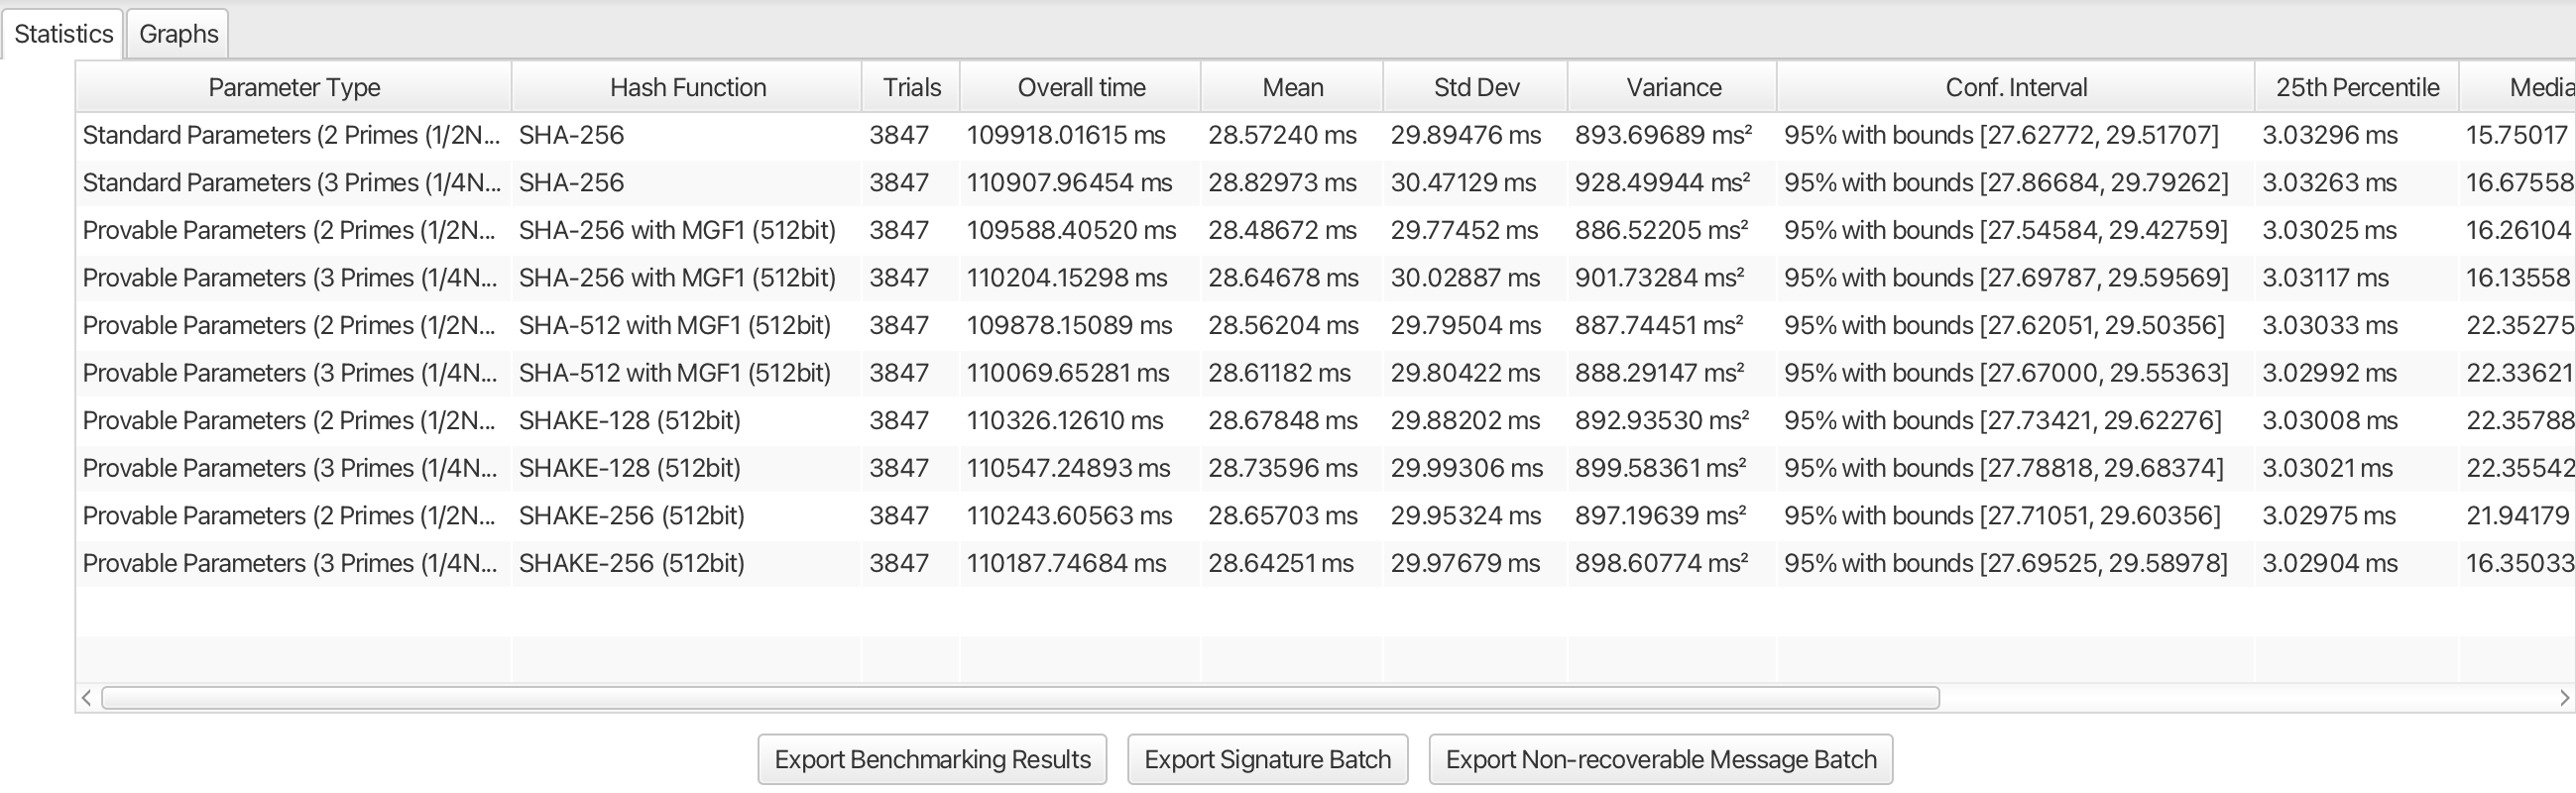
\includegraphics[width=\textwidth]{main_pictures/iso/iso_sign_1024bit_table1_1.png}} 
        \fbox{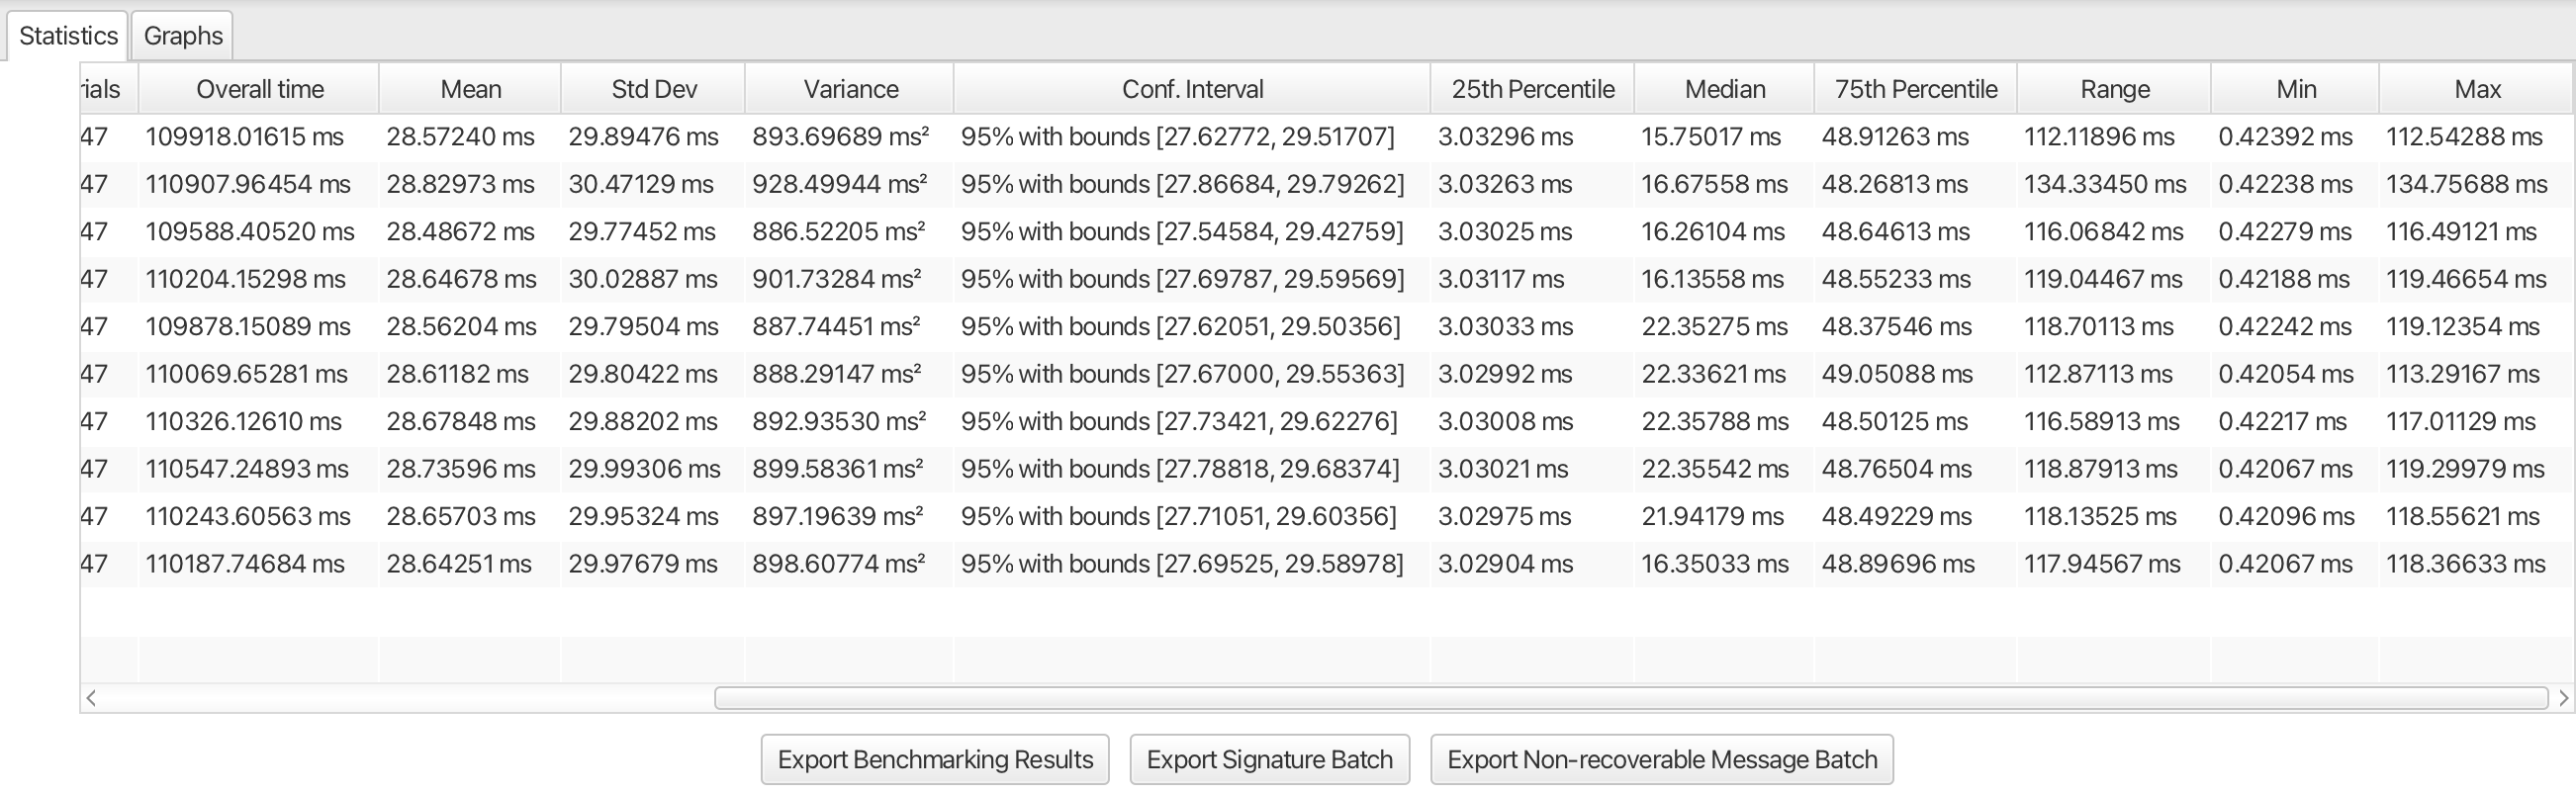
\includegraphics[width=\textwidth]{main_pictures/iso/iso_sign_1024bit_table2_1.png}}
    \end{minipage}
            \label{iso_sign_1024bit_table}
  \end{figure}
  
\begin{figure}[H]
    \centering % Center the images
     \caption{Instantiation of ISO/IEC 9796-2:2010 Signature Scheme 1 with standard vs provably secure parameters (2048-bit Key Size) for signature creation}
    % First image in a minipage
    \begin{minipage}{\textwidth}
        \centering
        \fbox{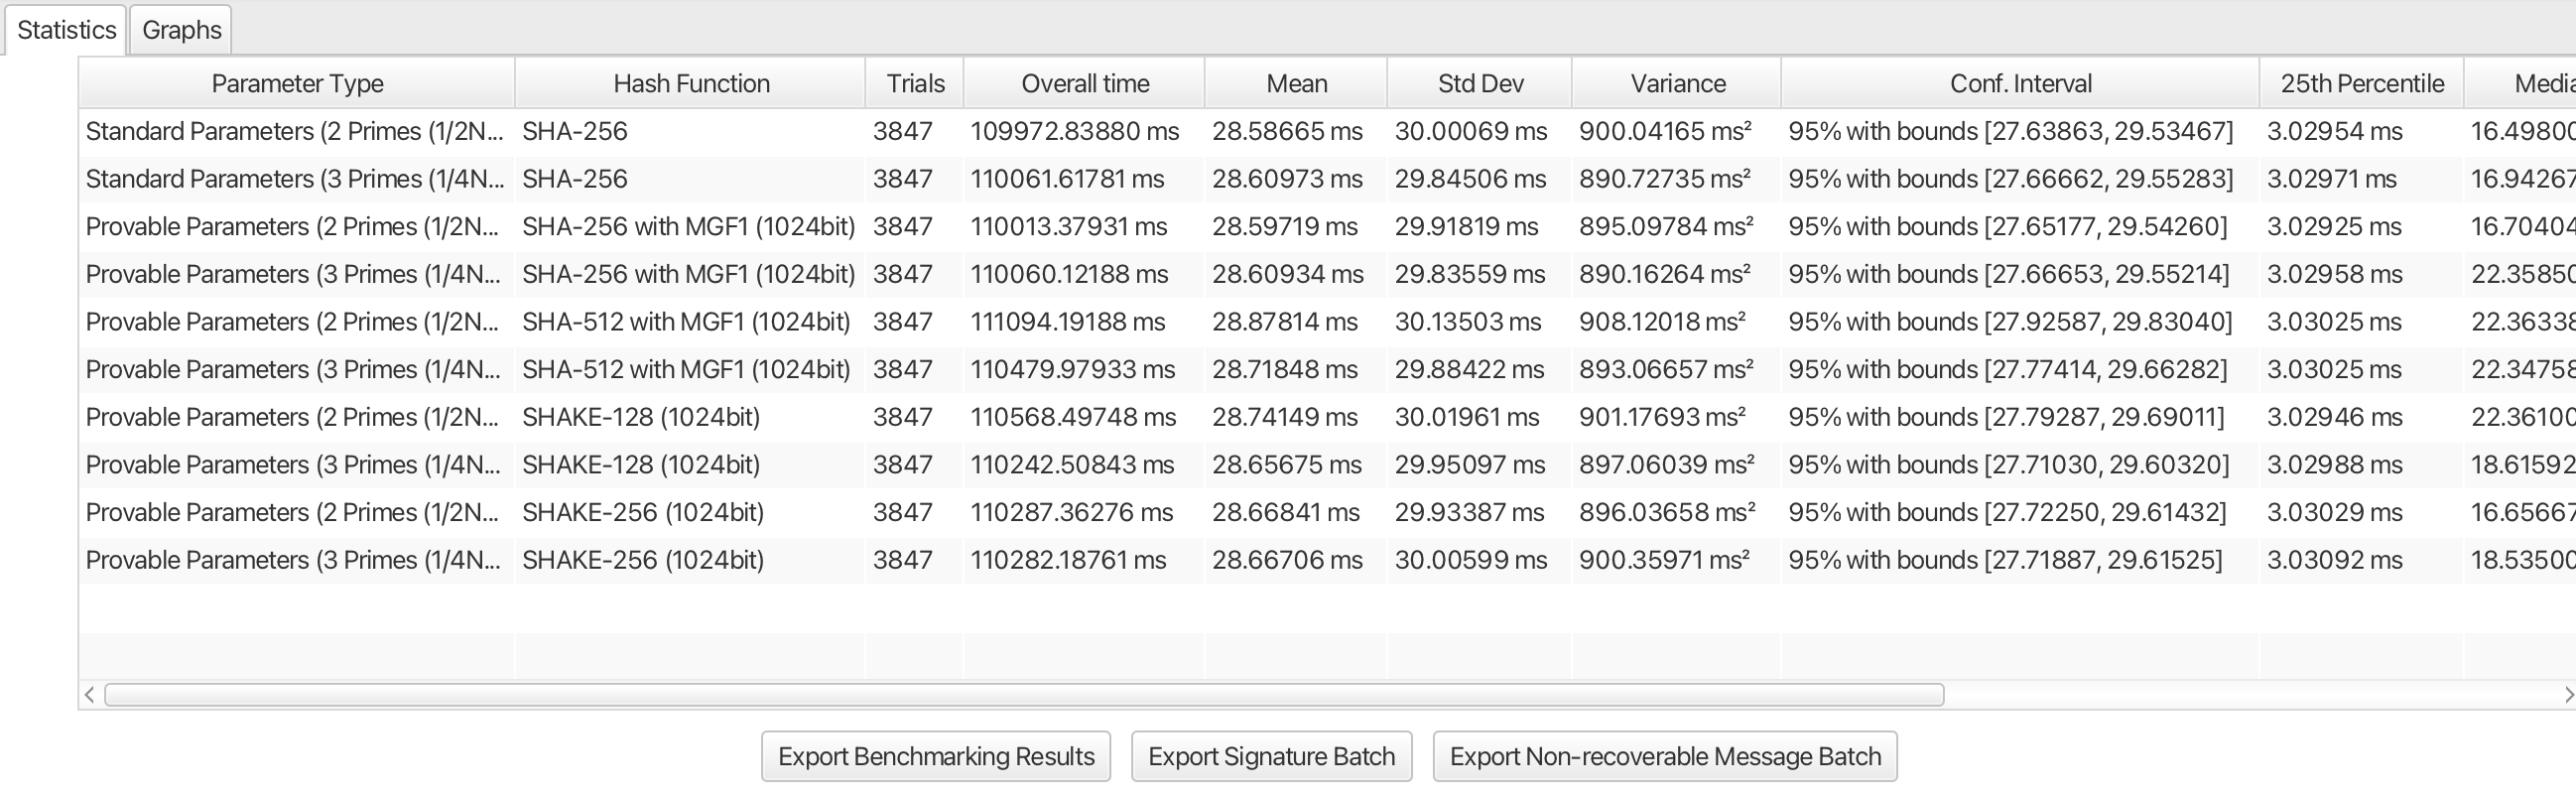
\includegraphics[width=\textwidth]{main_pictures/iso/iso_sign_2048bit_table1_1.png}} 
        \fbox{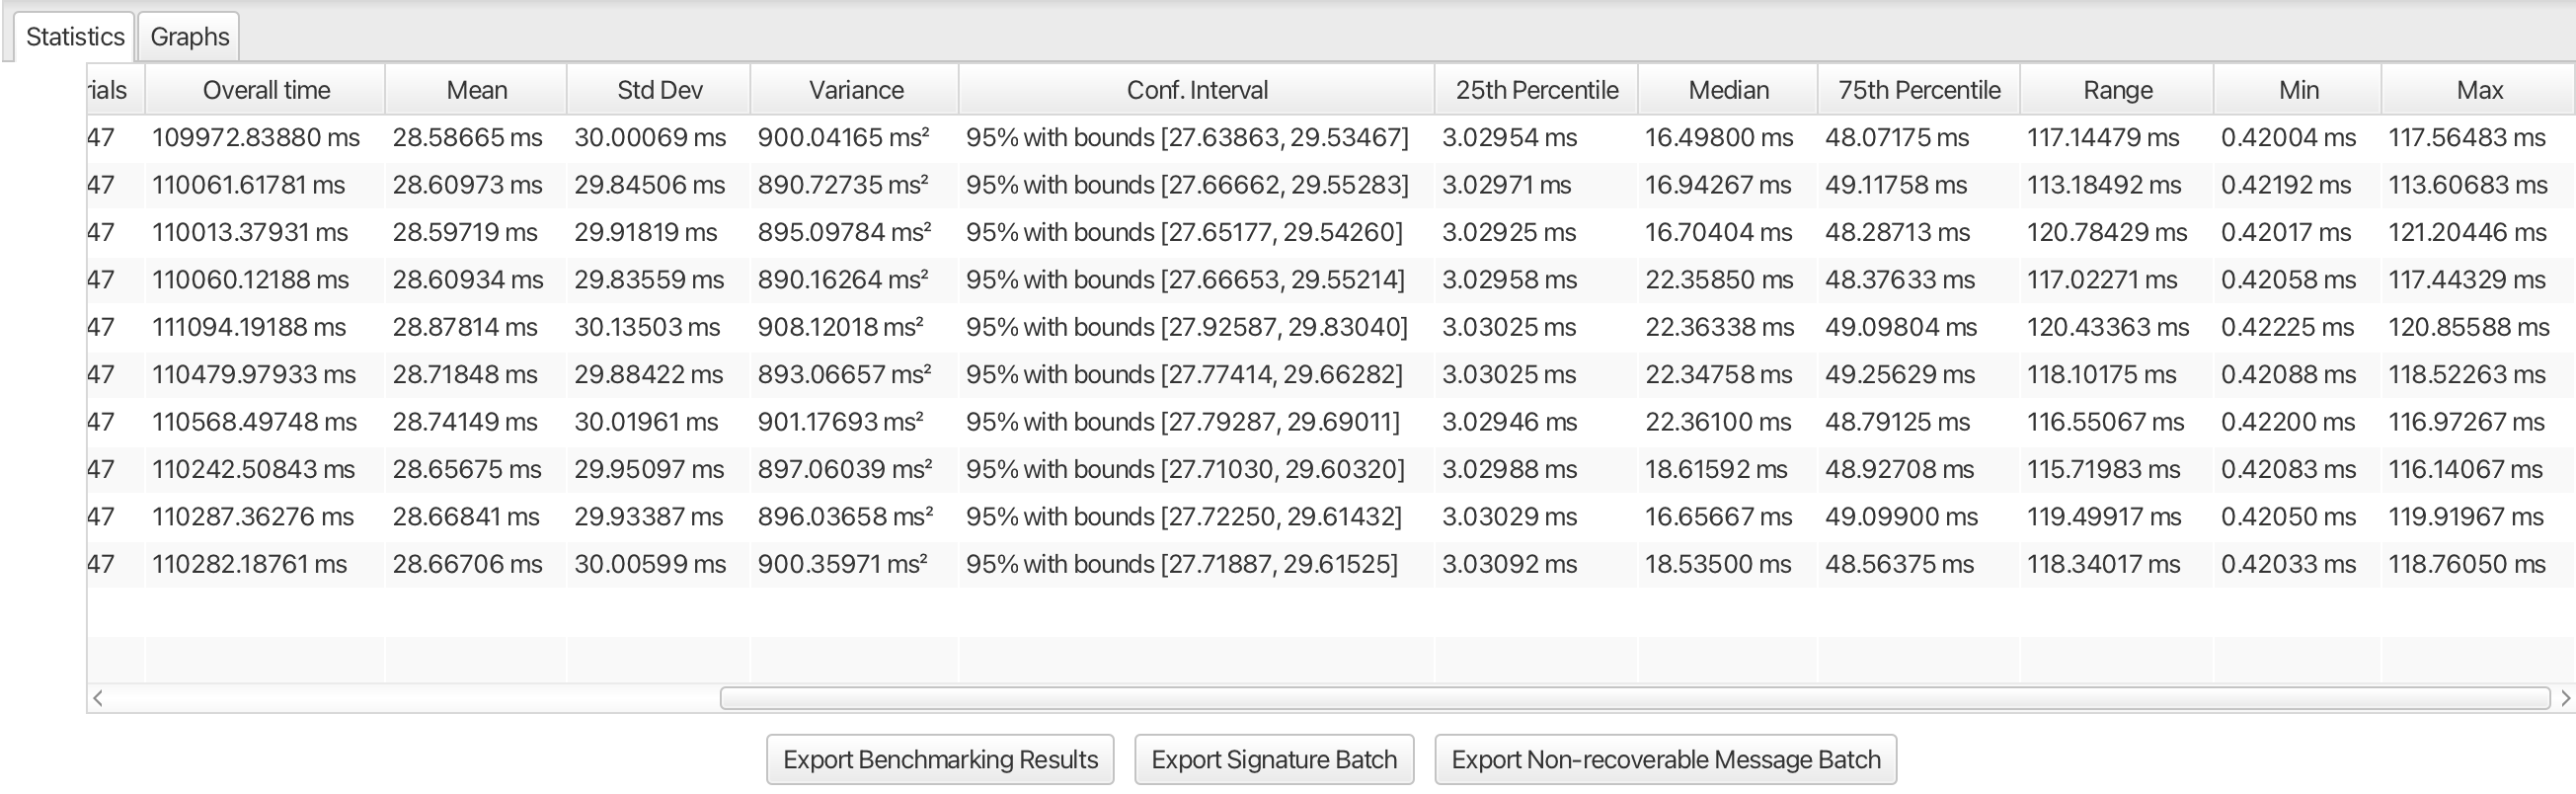
\includegraphics[width=\textwidth]{main_pictures/iso/iso_sign_2048bit_table2_1.png}}
    \end{minipage}
            \label{iso_sign_2048bit_table}
  \end{figure}
  
\begin{figure}[H]
    \centering % Center the images
     \caption{Instantiation of ISO/IEC 9796-2:2010 Signature Scheme 1 with standard vs provably secure parameters (3072-bit Key Size) for signature creation}
    % First image in a minipage
    \begin{minipage}{\textwidth}
        \centering
        \fbox{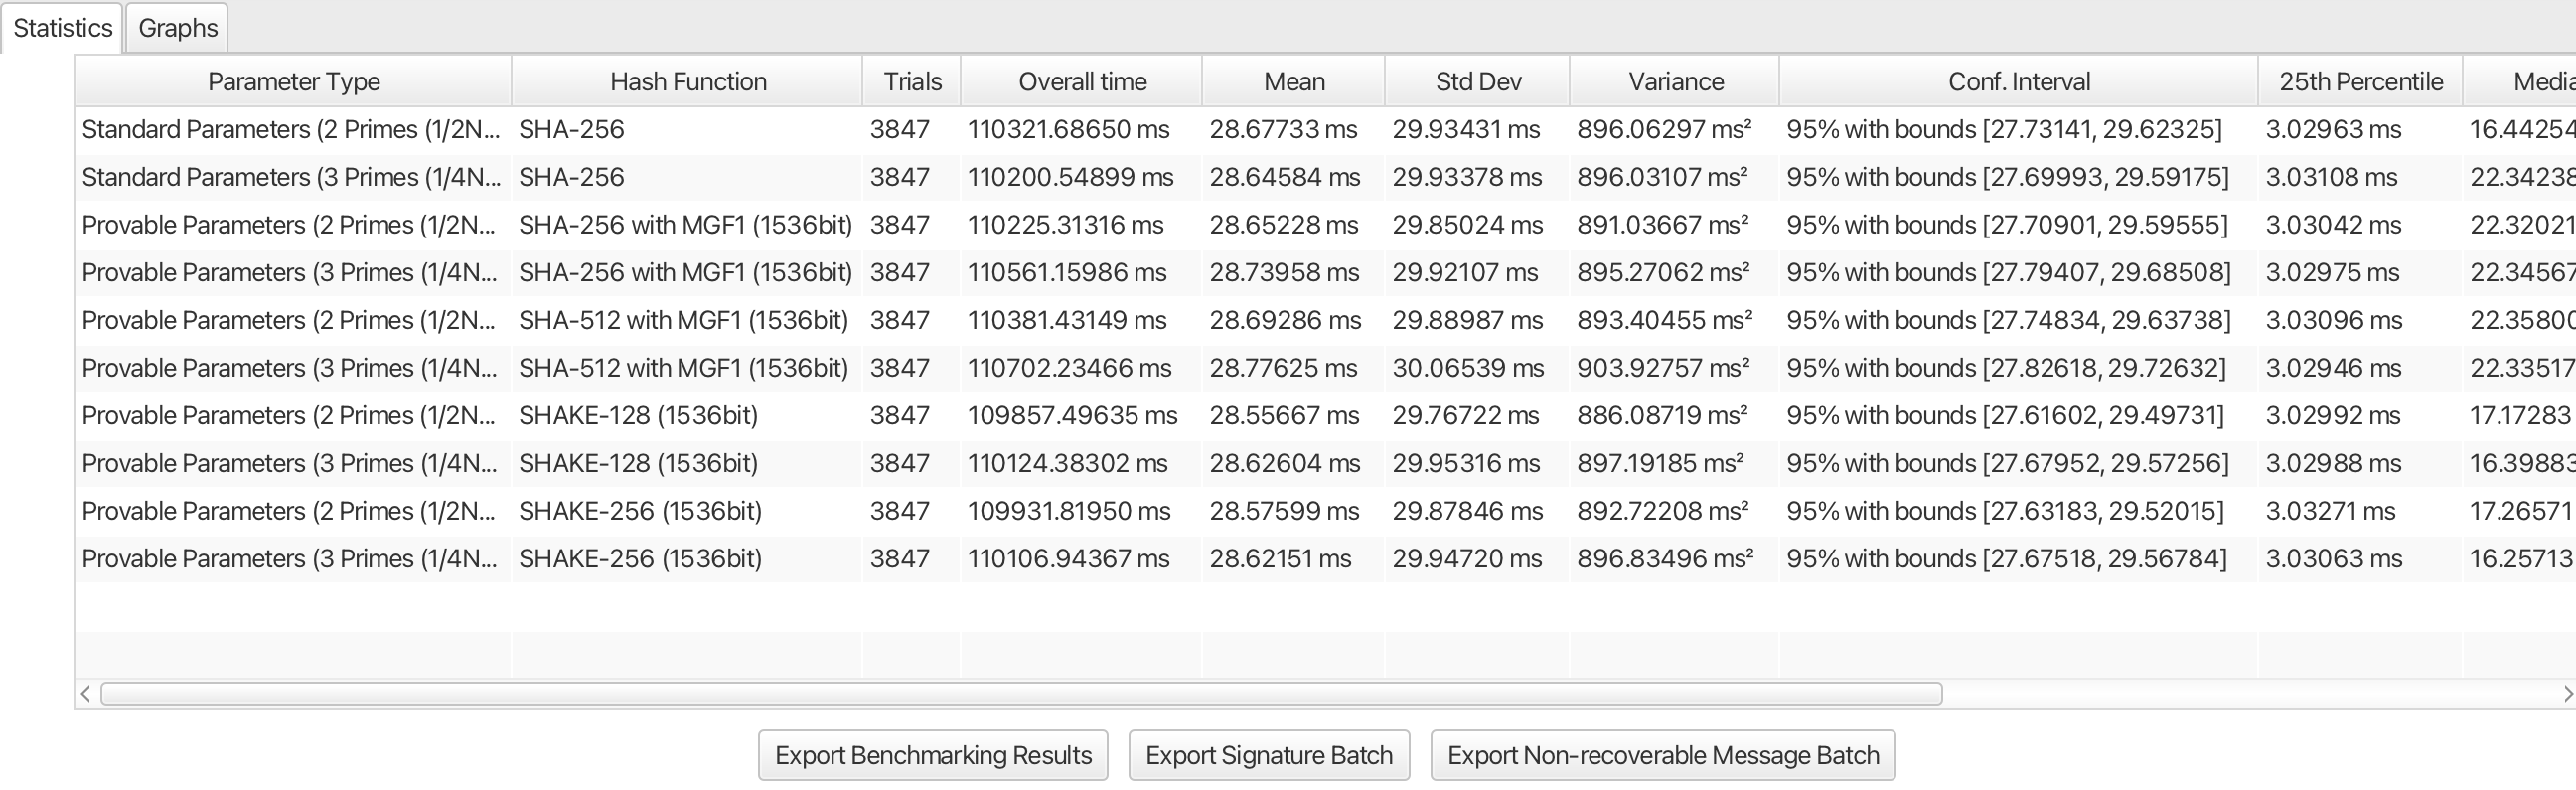
\includegraphics[width=\textwidth]{main_pictures/iso/iso_sign_3072bit_table1_1.png}} 
        \fbox{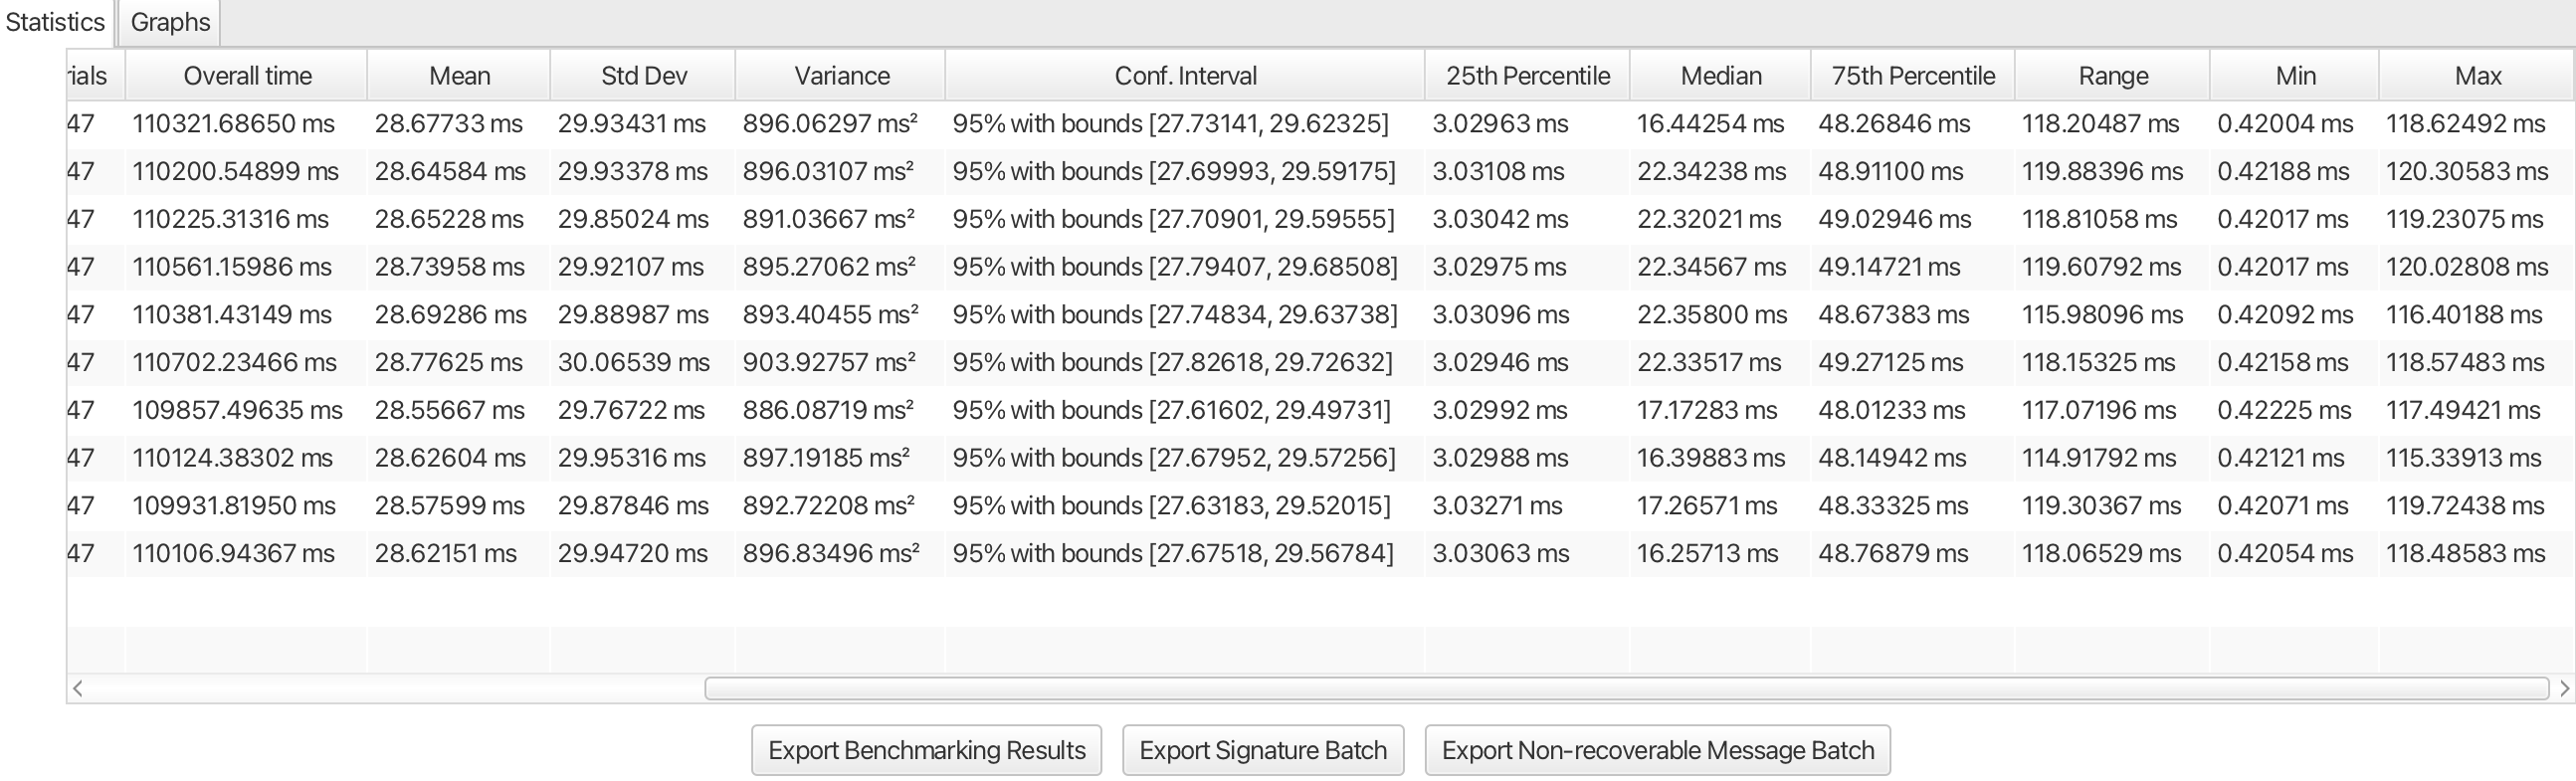
\includegraphics[width=\textwidth]{main_pictures/iso/iso_sign_3072bit_table2_1.png}}
    \end{minipage}
         \label{iso_sign_3072bit_table}
\end{figure}

\begin{figure}[H]
    \centering % Center the images
     \caption{Instantiation of ISO/IEC 9796-2:2010 Signature Scheme 1 with standard vs provably secure parameters (4096-bit Key Size) for signature creation}
    % First image in a minipage
    \begin{minipage}{\textwidth}
        \centering
        \fbox{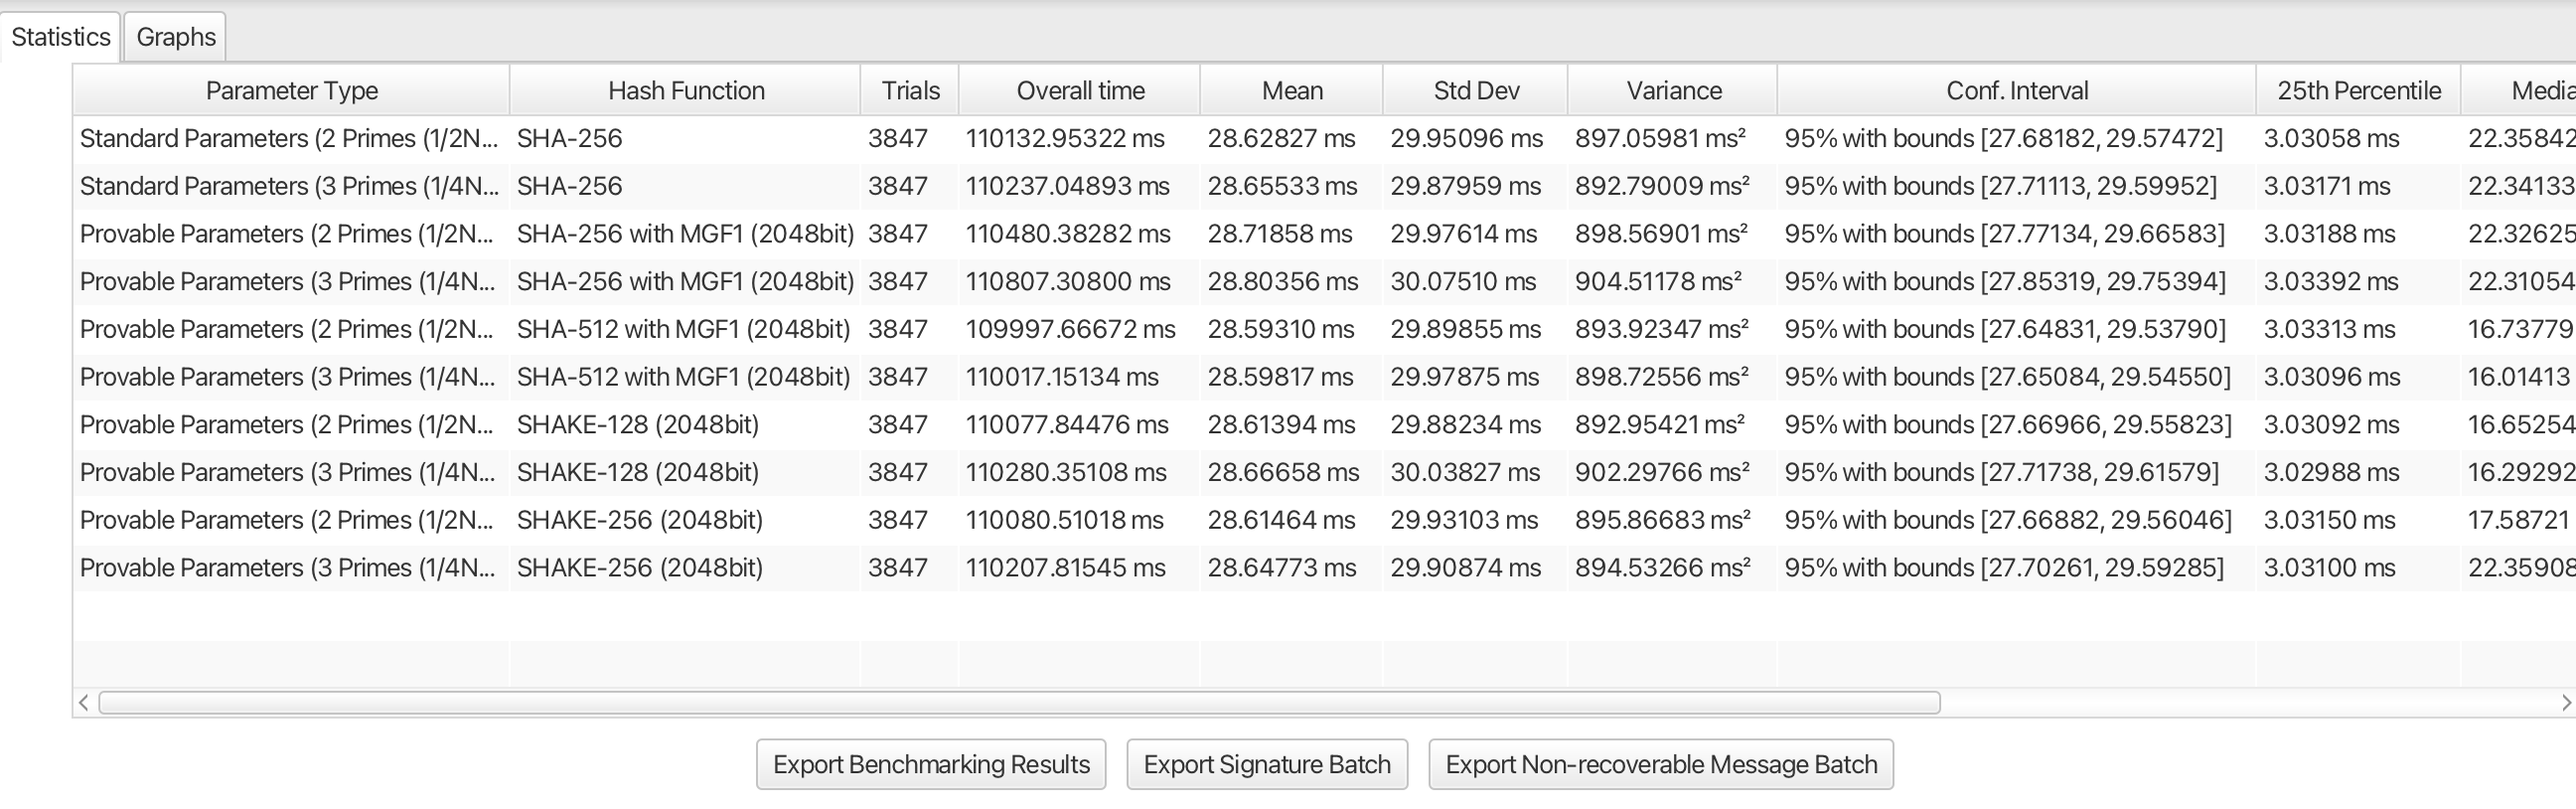
\includegraphics[width=\textwidth]{main_pictures/iso/iso_sign_4096bit_table1_1.png}} 
        \fbox{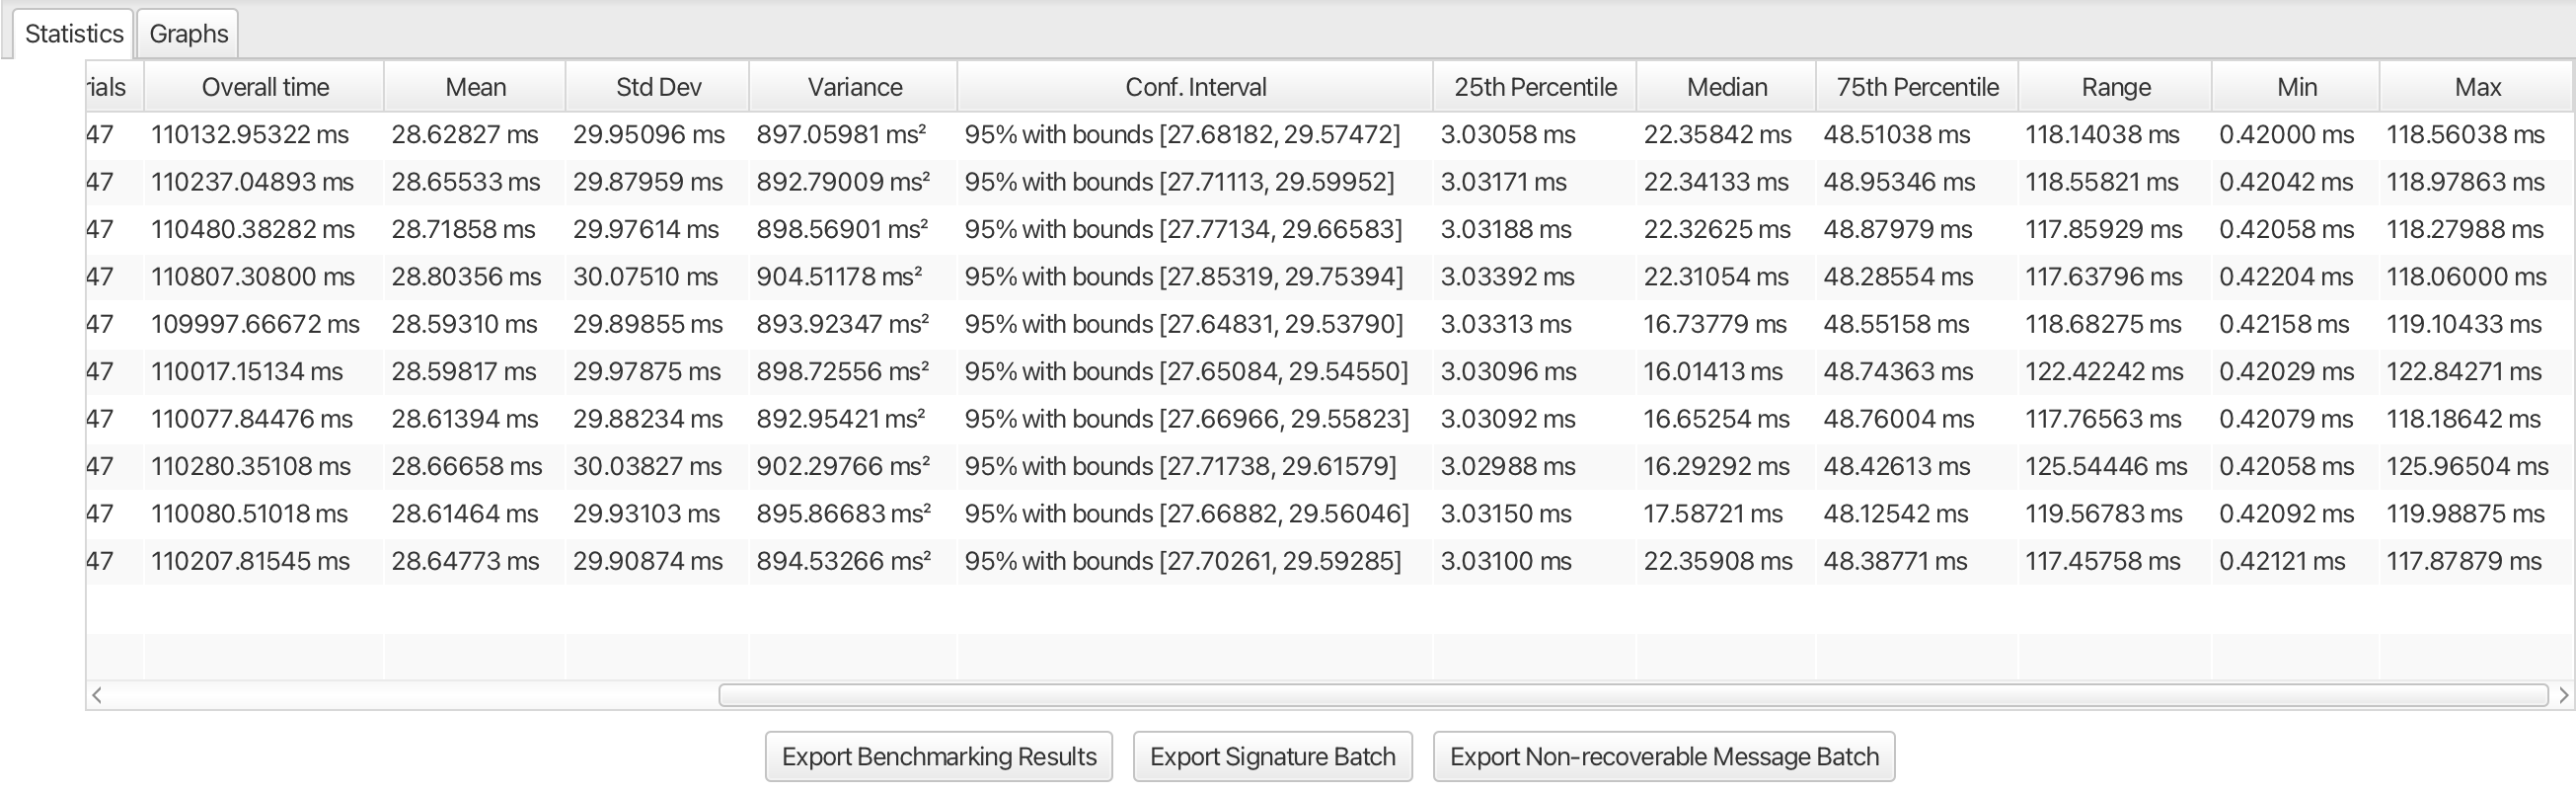
\includegraphics[width=\textwidth]{main_pictures/iso/iso_sign_4096bit_table2_1.png}}
    \end{minipage}
             \label{iso_sign_4096bit_table}
\end{figure}

\begin{figure}[H]
    \centering % Center the images
     \caption{Instantiation of ISO/IEC 9796-2:2010 Signature Scheme 1 with standard vs provably secure parameters (5120-bit Key Size) for signature creation}
    % First image in a minipage
    \begin{minipage}{\textwidth}
        \centering
        \fbox{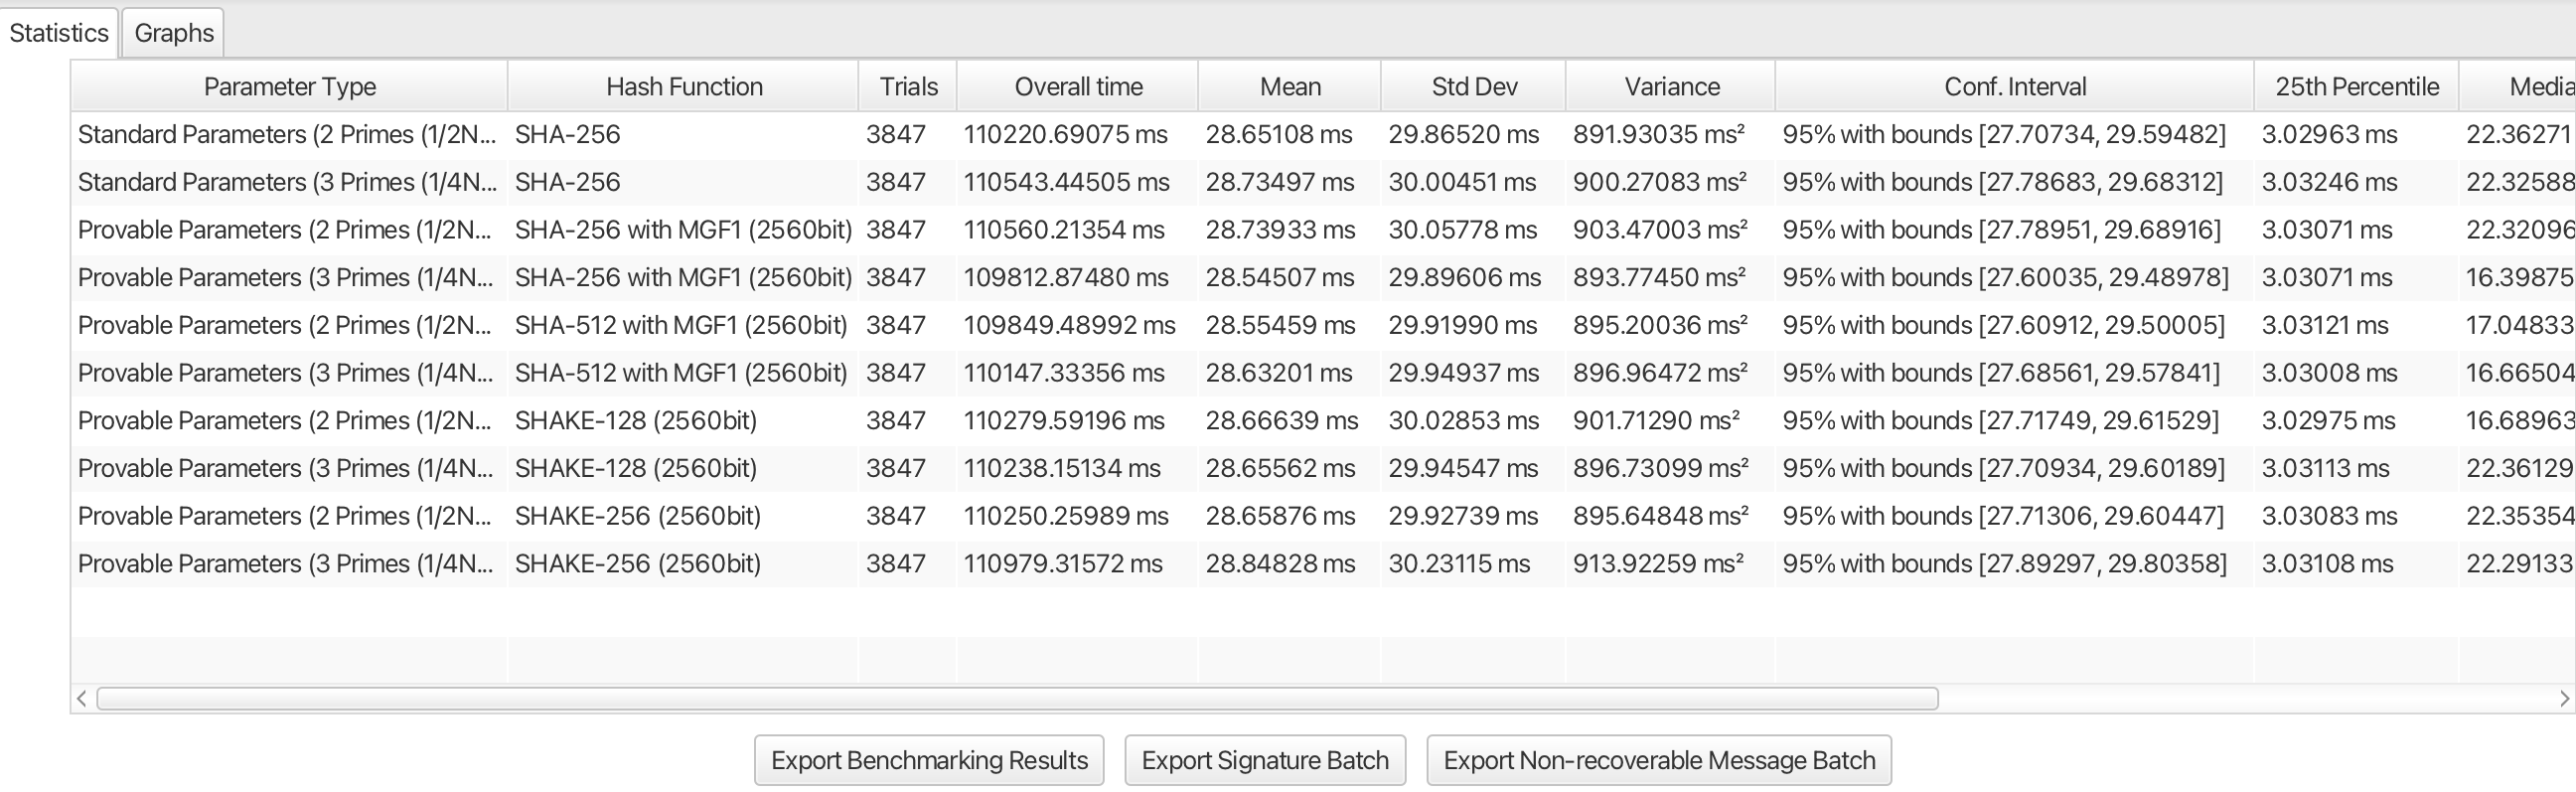
\includegraphics[width=\textwidth]{main_pictures/iso/iso_sign_5120bit_table1_1.png}} 
        \fbox{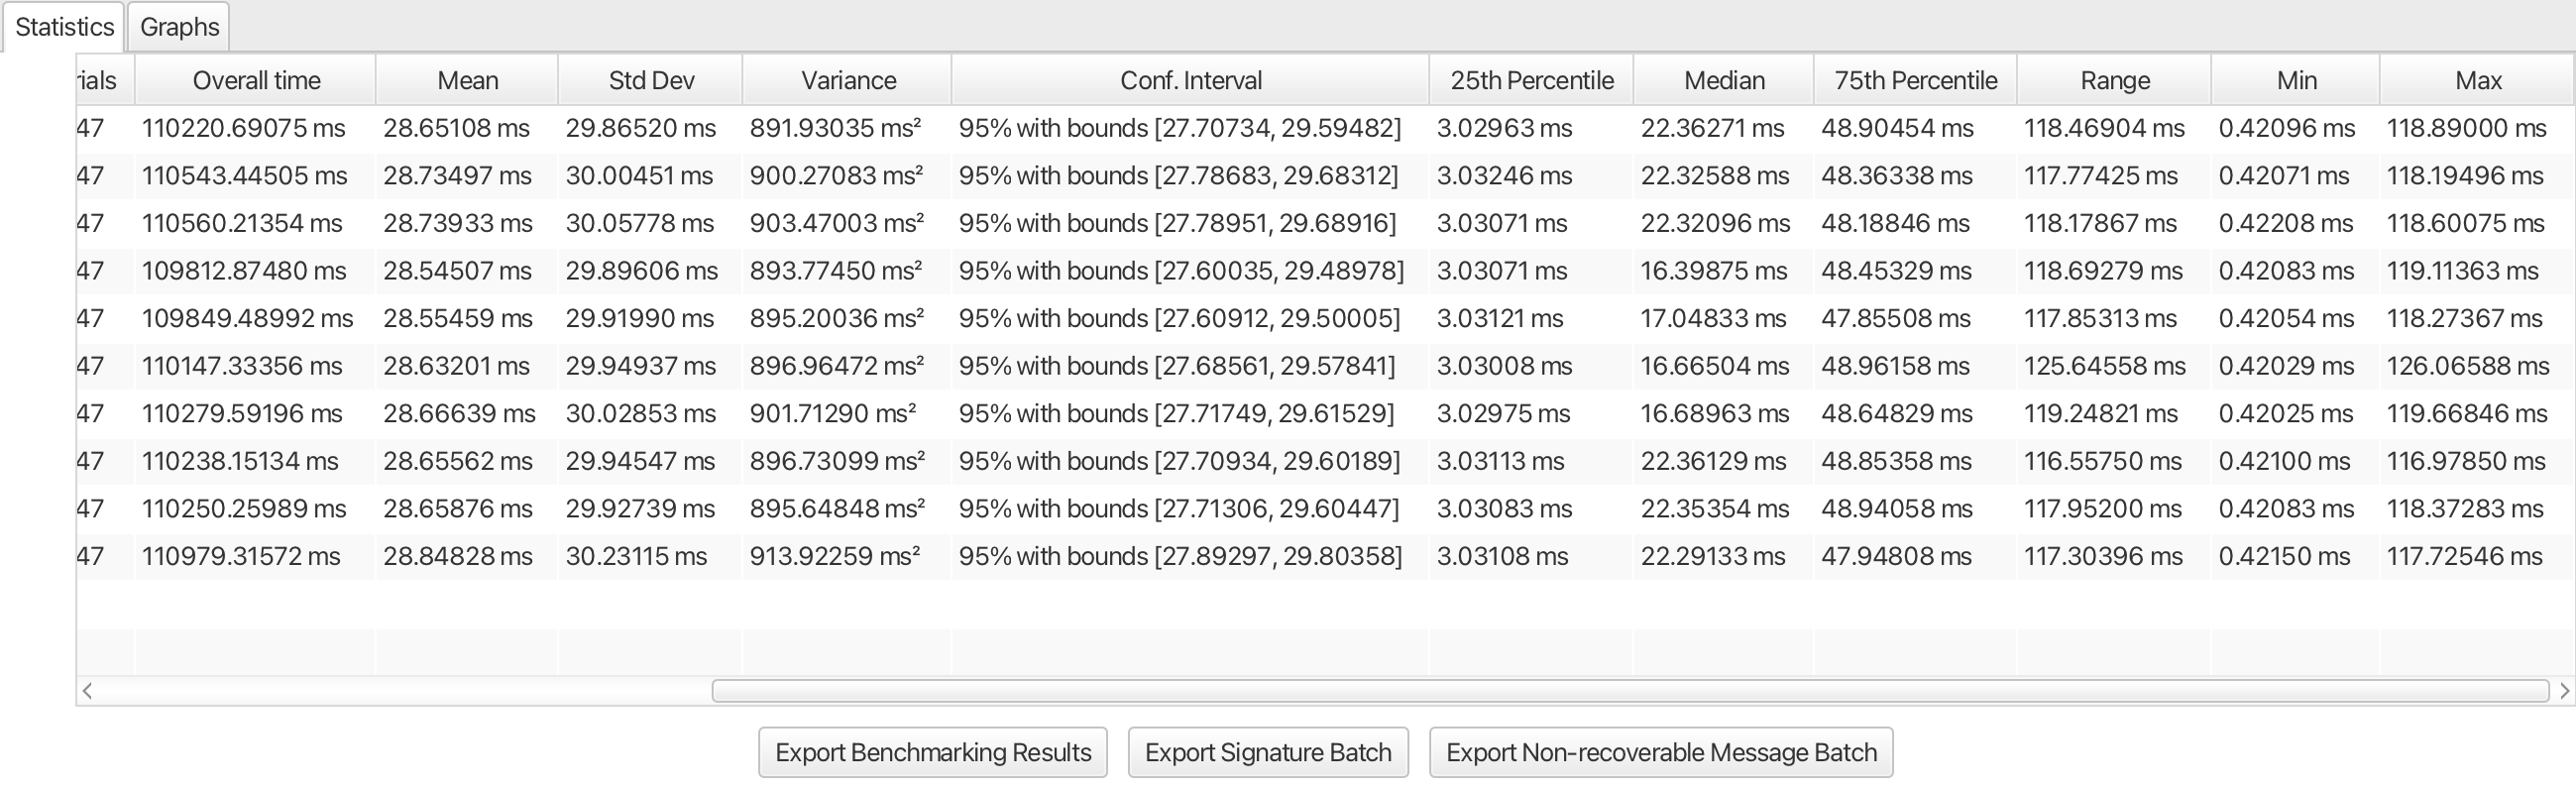
\includegraphics[width=\textwidth]{main_pictures/iso/iso_sign_5120bit_table2_1.png}}
    \end{minipage}
     \label{iso_sign_5120bit_table}
\end{figure}

\begin{figure}[H]
    \centering % Center the images
     \caption{Instantiation of ISO/IEC 9796-2:2010 Signature Scheme 1 with standard vs provably secure parameters (6144-bit Key Size) for signature creation}
    % First image in a minipage
    \begin{minipage}{\textwidth}
        \centering
        \fbox{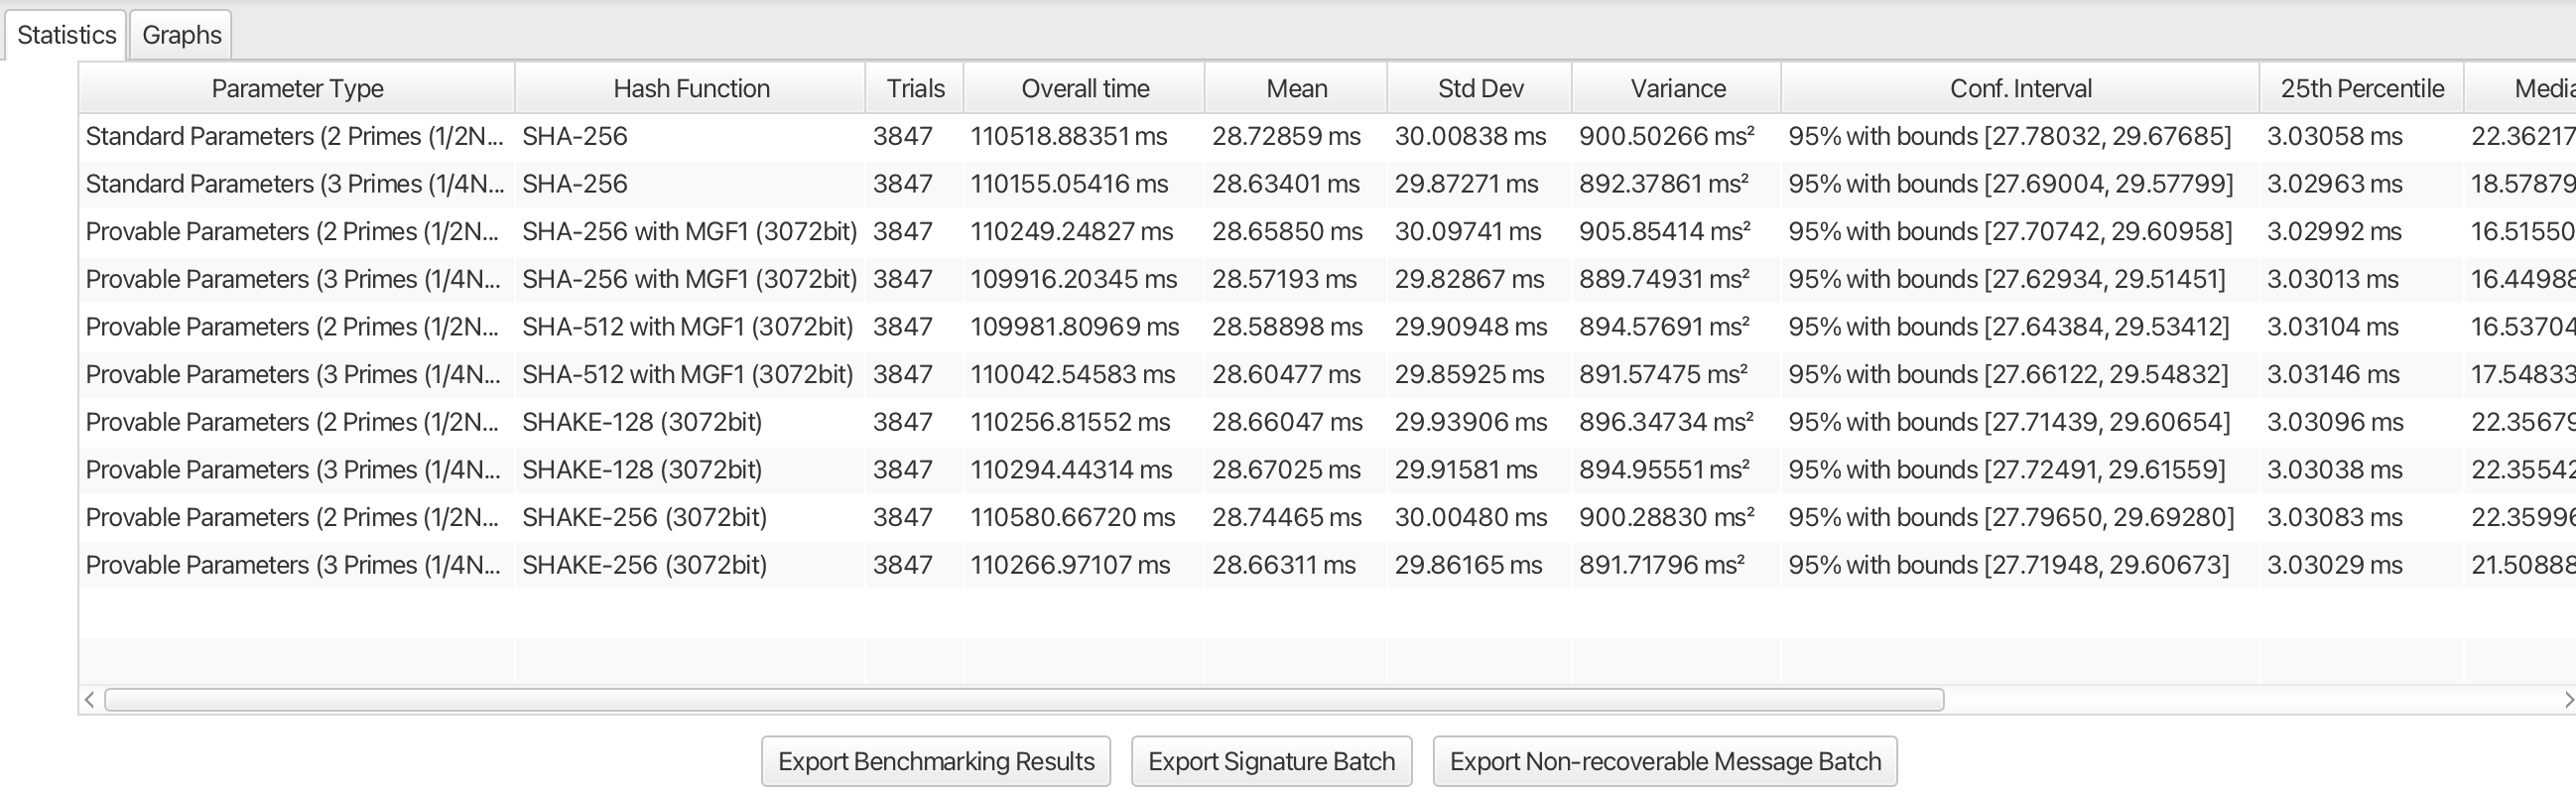
\includegraphics[width=\textwidth]{main_pictures/iso/iso_sign_6144bit_table1_1.png}} 
        \fbox{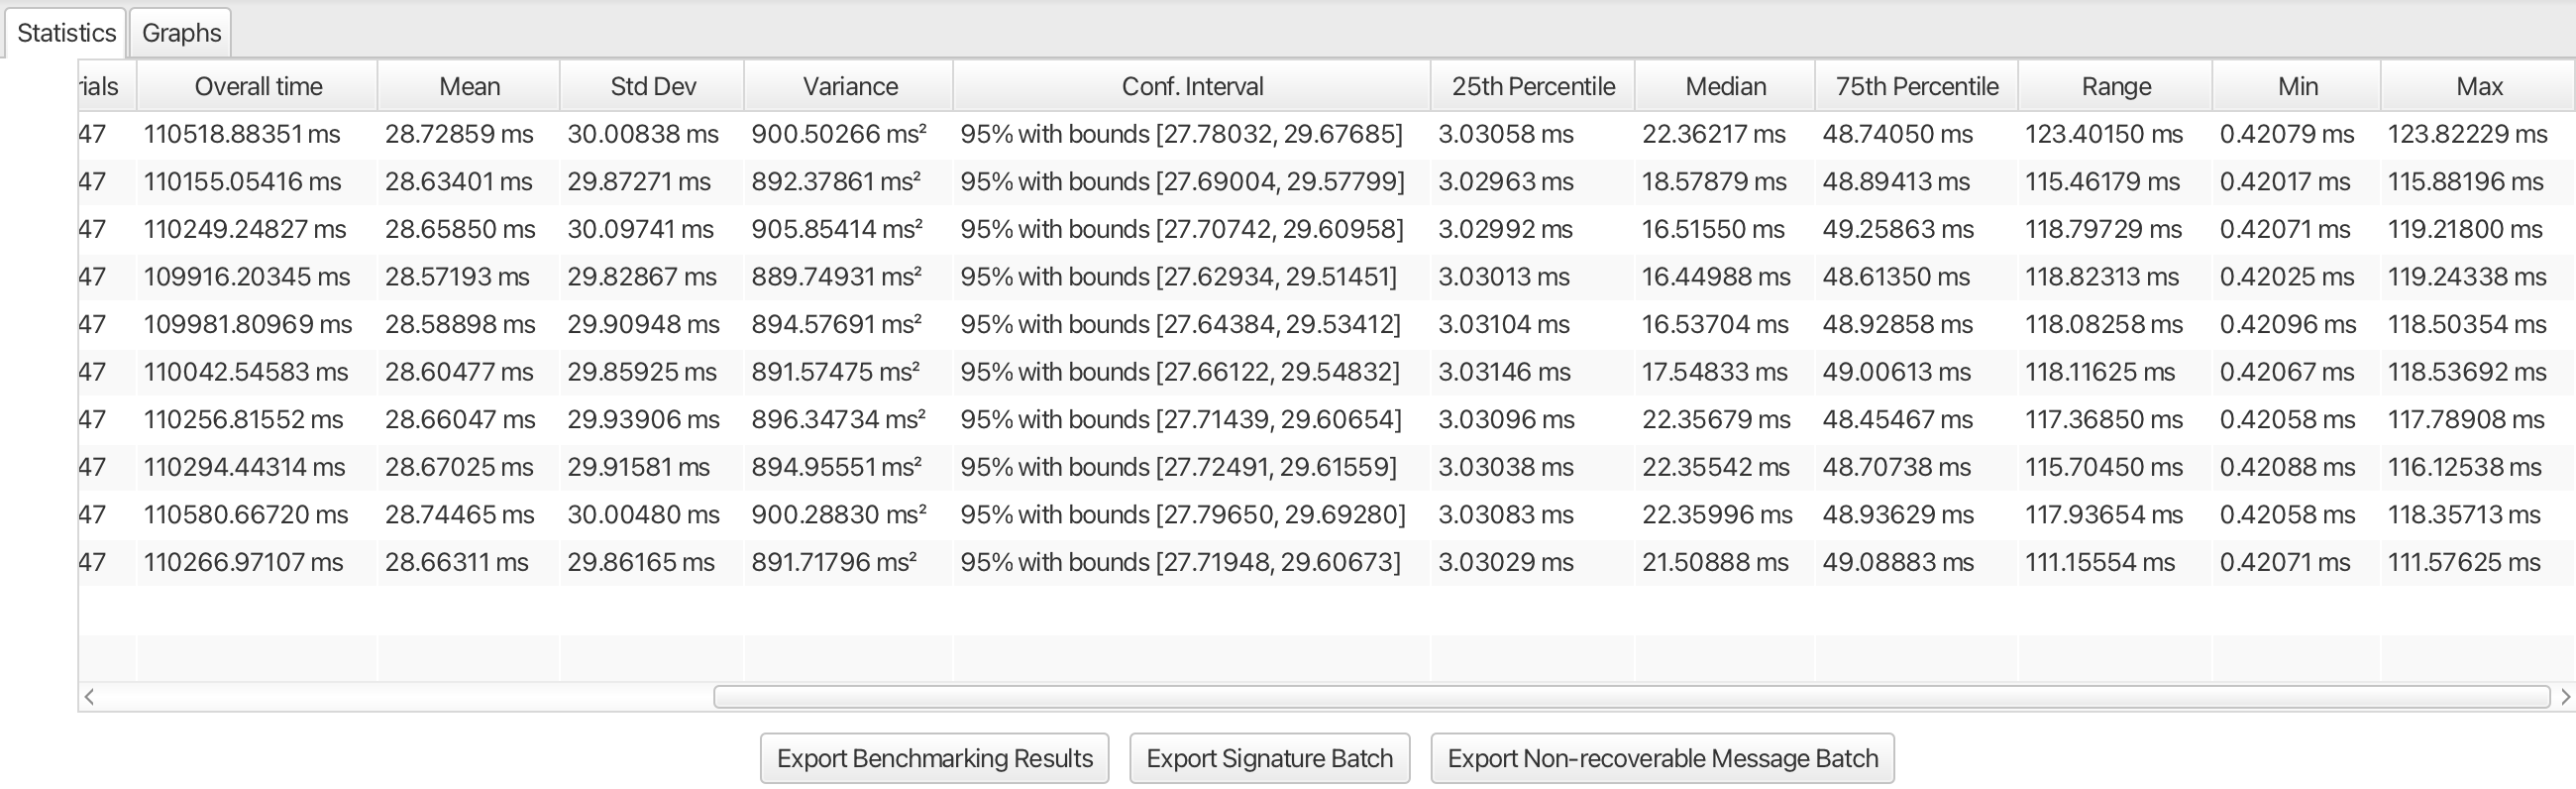
\includegraphics[width=\textwidth]{main_pictures/iso/iso_sign_6144bit_table2_1.png}}
    \end{minipage}
         \label{iso_sign_6144bit_table}
\end{figure}
\end{comment}

\begin{landscape}
\pagestyle{empty}%
\section{Signature Creation Results (ISO/IEC 9796-2:2010 Signature Scheme 1)}

\begin{longtable}{|p{2.3cm}|p{1.8cm}|p{1.0cm}|p{1.7cm}|p{1.4cm}|p{1.5cm}|p{1.8cm}|p{1.5cm}|p{1.2cm}|p{1.5cm}|p{1.3cm}|p{1.2cm}|p{1.3cm}|p{1.3cm}|}

\caption{\textbf{Instantiation of ISO/IEC 9796-2:2010 Signature Scheme 1 with Standard vs Provably Secure Parameters (1024-bit Key Size) for Signature Creation}}
     \label{iso_sign_1024bit_table} \\
\hline
\textbf{Parameter Type} & \textbf{Hash Function} & \textbf{Trials} & \textbf{Overall Time} & \textbf{Mean} & \textbf{Std Dev} & \textbf{Variance} & \textbf{Conf. Interval} & \textbf{25th Percentile} & \textbf{Median} & \textbf{75th Percentile} & \textbf{Range} & \textbf{Min} & \textbf{Max} \\
\hline
\endfirsthead

\multicolumn{14}{c}%
{{\bfseries \tablename\ \thetable{} -- Signature Creation Results for ISO/IEC 9796-2 Scheme 1 with 1024-bit Key Size (continued from previous page)}} \\
\hline
\textbf{Parameter Type} & \textbf{Hash Function} & \textbf{Trials} & \textbf{Overall Time} & \textbf{Mean} & \textbf{Std Dev} & \textbf{Variance} & \textbf{Conf. Interval} & \textbf{25th Percentile} & \textbf{Median} & \textbf{75th Percentile} & \textbf{Range} & \textbf{Min} & \textbf{Max} \\
\hline
\endhead

\hline \multicolumn{14}{|r|}{{Continued on next page}} \\ \hline
\endfoot

\hline
\endlastfoot

Standard Parameters (2 Primes) & SHA-256 & 3847 & 109918.
01615 ms & 28.57240 ms & 29.89476 ms & 893.69689 ms\textsuperscript{2}  & 95\% with bounds 27.62772 ms - 29.51707 ms & 3.03296 ms & 15.75017 ms & 48.91263 ms & 112.
11896 ms & 0.42392 ms & 112.
54288 ms \\
\hline
Standard Parameters (3 Primes) & SHA-256 & 3847 & 110907.
96454 ms & 28.82973 ms & 30.47129 ms & 928.49944 ms\textsuperscript{2}  & 95\% with bounds 27.86684 ms - 29.79262 ms & 3.03263 ms & 16.67558 ms & 48.
26813 ms & 134.33450 ms & 0.42238 ms & 134.
75688 ms \\
\hline
Provable Parameters (2 Primes) & SHA-256 with MGF1 (512bit) & 3847 & 109588.
40520 ms & 28.48672 ms & 29.77452 ms & 886.52205 ms\textsuperscript{2}  & 95\% with bounds 27.54584 ms - 29.42759 ms & 3.03025 ms & 16.26104 ms & 48.
64613 ms & 116.06842 ms & 0.42279 ms & 116.
49121 ms \\
\hline
Provable Parameters (3 Primes) & SHA-256 with MGF1 (512bit) & 3847 & 110204.
15298 ms & 28.64678 ms & 30.02887 ms & 901.73284 ms\textsuperscript{2}  & 95\% with bounds 27.69787 ms - 29.59569 ms & 3.03117 ms & 16.
13558 ms & 48.55233 ms & 119.04467 ms & 0.42188 ms & 119.
46654 ms \\
\hline
Provable Parameters (2 Primes) & SHA-512 with MGF1 (512bit) & 3847 & 109878.
15089 ms & 28.56204 ms & 29.79504 ms & 887.74451 ms\textsuperscript{2}  & 95\% with bounds 27.62051 ms - 29.50356 ms & 3.03033 ms & 22.35275 ms & 48.
37546 ms & 118.70113 ms & 0.42242 ms & 119.
12354 ms \\
\hline
Provable Parameters (3 Primes) & SHA-512 with MGF1 (512bit) & 3847 & 110069.
65281 ms & 28.61182 ms & 29.80422 ms & 888.29147 ms\textsuperscript{2}  & 95\% with bounds 27.67000 ms - 29.55363 ms & 3.02992 ms & 22.33621 ms & 49.
05088 ms & 112.87113 ms & 0.42054 ms & 113.
29167 ms \\
\hline
Provable Parameters (2 Primes) & SHAKE-128 (512bit) & 3847 & 110326.
12610 ms & 28.67848 ms & 29.88202 ms & 892.93530 ms\textsuperscript{2}  & 95\% with bounds 27.73421 ms - 29.62276 ms & 3.03008 ms & 22.35788 ms & 48.50125 ms & 116.
58913 ms & 0.42217 ms & 117.
01129 ms \\
\hline
Provable Parameters (3 Primes) & SHAKE-128 (512bit) & 3847 & 110547.
24893 ms & 28.73596 ms & 29.99306 ms & 899.58361 ms\textsuperscript{2}  & 95\% with bounds 27.78818 ms - 29.68374 ms & 3.03021 ms & 22.35542 ms & 48.
76504 ms & 118.87913 ms & 0.42067 ms & 119.
29979 ms \\
\hline
Provable Parameters (2 Primes) & SHAKE-256 (512bit) & 3847 & 110243.
60563 ms & 28.65703 ms & 29.95324 ms & 897.19639 ms\textsuperscript{2}  & 95\% with bounds 27.71051 ms - 29.60356 ms & 3.02975 ms & 21.94179 ms & 48.49229 ms & 118.
13525 ms & 0.42096 ms & 118.
55621 ms \\
\hline
Provable Parameters (3 Primes) & SHAKE-256 (512bit) & 3847 & 110187.
74684 ms & 28.64251 ms & 29.97679 ms & 898.60774 ms\textsuperscript{2}  & 95\% with bounds 27.69525 ms - 29.58978 ms & 3.02904 ms & 16.35033 ms & 48.
89696 ms & 117.94567 ms & 0.42067 ms & 118.
36633 ms \\
\hline



\end{longtable}

\begin{longtable}{|p{2.3cm}|p{1.8cm}|p{1.0cm}|p{1.7cm}|p{1.4cm}|p{1.5cm}|p{1.8cm}|p{1.5cm}|p{1.2cm}|p{1.5cm}|p{1.3cm}|p{1.2cm}|p{1.3cm}|p{1.3cm}|}

\caption{\textbf{Instantiation of ISO/IEC 9796-2:2010 Signature Scheme 1 with Standard vs Provably Secure Parameters (2048-bit Key Size) for Signature Creation}}
     \label{iso_sign_2048bit_table} \\
\hline
\textbf{Parameter Type} & \textbf{Hash Function} & \textbf{Trials} & \textbf{Overall Time} & \textbf{Mean} & \textbf{Std Dev} & \textbf{Variance} & \textbf{Conf. Interval} & \textbf{25th Percentile} & \textbf{Median} & \textbf{75th Percentile} & \textbf{Range} & \textbf{Min} & \textbf{Max} \\
\hline
\endfirsthead

\multicolumn{14}{c}%
{{\bfseries \tablename\ \thetable{} -- Signature Creation Results for ISO/IEC 9796-2 Scheme 1 with 2048-bit Key Size (continued from previous page)}} \\
\hline
\textbf{Parameter Type} & \textbf{Hash Function} & \textbf{Trials} & \textbf{Overall Time} & \textbf{Mean} & \textbf{Std Dev} & \textbf{Variance} & \textbf{Conf. Interval} & \textbf{25th Percentile} & \textbf{Median} & \textbf{75th Percentile} & \textbf{Range} & \textbf{Min} & \textbf{Max} \\
\hline
\endhead

\hline \multicolumn{14}{|r|}{{Continued on next page}} \\ \hline
\endfoot

\hline
\endlastfoot
Standard Parameters (2 Primes) & SHA-256 & 3847 & 109972.
83880 ms & 28.58665 ms & 30.00069 ms & 900.04165 ms\textsuperscript{2} & 95\% with bounds 27.63863 ms - 29.53467 ms & 3.02954 ms & 16.49800 ms & 48.07175 ms & 117.
14479 ms & 0.42004 ms & 117.
56483 ms  \\
\hline
Standard Parameters (3 Primes) & SHA-256 & 3847 & 110061.
61781 ms & 28.60973 ms & 29.84506 ms & 890.72735 ms\textsuperscript{2} & 95\% with bounds 27.66662 ms - 29.55283 ms & 3.02971 ms & 16.94267 ms & 49.11758 ms & 113.
18492 ms & 0.42192 ms & 113.
60683 ms  \\
\hline
Provable Parameters (2 Primes) & SHA-256 with MGF1 (1024bit) & 3847 & 110013.
37931 ms & 28.59719 ms & 29.91819 ms & 895.09784 ms\textsuperscript{2} & 95\% with bounds 27.65177 ms - 29.54260 ms & 3.02925 ms & 16.70404 ms & 48.28713 ms & 120.
78429 ms & 0.42017 ms & 121.
20446 ms  \\
\hline
Provable Parameters (3 Primes) & SHA-256 with MGF1 (1024bit) & 3847 & 110060.12188 ms & 28.60934 ms & 29.83559 ms & 890.16264 ms\textsuperscript{2} & 95\% with bounds 27.66653 ms - 29.55214 ms & 3.02958 ms & 22.35850 ms & 48.37633 ms & 117.
02271 ms & 0.42058 ms & 117.
44329 ms  \\
\hline
Provable Parameters (2 Primes) & SHA-512 with MGF1 (1024bit) & 3847 & 111094.
19188 ms & 28.87814 ms & 30.13503 ms & 908.12018 ms\textsuperscript{2} & 95\% with bounds 27.92587 ms - 29.83040 ms & 3.03025 ms & 22.36338 ms & 49.09804 ms & 120.
43363 ms & 0.42225 ms & 120.
85588 ms  \\
\hline
Provable Parameters (3 Primes) & SHA-512 with MGF1 (1024bit) & 3847 & 110479.
97933 ms & 28.71848 ms & 29.88422 ms & 893.06657 ms\textsuperscript{2} & 95\% with bounds 27.77414 ms - 29.66282 ms & 3.03025 ms & 22.34758 ms & 49.25629 ms & 118.
10175 ms & 0.42088 ms & 118.
52263 ms  \\
\hline
Provable Parameters (2 Primes) & SHAKE-128 (1024bit) & 3847 & 110568.
49748 ms & 28.74149 ms & 30.01961 ms & 901.17693 ms\textsuperscript{2} & 95\% with bounds 27.79287 ms - 29.69011 ms & 3.02946 ms & 22.36100 ms & 48.79125 ms & 116.
55067 ms & 0.42200 ms & 116.
97267 ms  \\
\hline
Provable Parameters (3 Primes) & SHAKE-128 (1024bit) & 3847 & 110242.
50843 ms & 28.65675 ms & 29.95097 ms & 897.06039 ms\textsuperscript{2} & 95\% with bounds 27.71030 ms - 29.60320 ms & 3.02988 ms & 18.61592 ms & 48.
92708 ms & 115.71983 ms & 0.42083 ms & 116.
14067 ms \\
\hline
Provable Parameters (2 Primes) & SHAKE-256 (1024bit) & 3847 & 110287.
36276 ms & 28.66841 ms & 29.93387 ms & 896.03658 ms\textsuperscript{2} & 95\% with bounds 27.72250 ms - 29.61432 ms & 3.03029 ms & 16.65667 ms & 49.09900 ms & 119.
49917 ms & 0.42050 ms & 119.
91967 ms  \\
\hline
Provable Parameters (3 Primes) & SHAKE-256 (1024bit) & 3847 & 110282.
18761 ms & 28.66706 ms & 30.00599 ms & 900.35971 ms\textsuperscript{2} & 95\% with bounds 27.71887 ms - 29.61525 ms & 3.03092 ms & 18.53500 ms & 48.56375 ms & 118.
34017 ms & 0.42033 ms & 118.
76050 ms  \\
\hline



\end{longtable}


\begin{longtable}{|p{2.3cm}|p{1.8cm}|p{1.0cm}|p{1.7cm}|p{1.4cm}|p{1.5cm}|p{1.8cm}|p{1.5cm}|p{1.2cm}|p{1.5cm}|p{1.3cm}|p{1.2cm}|p{1.3cm}|p{1.3cm}|}

\caption{\textbf{Instantiation of ISO/IEC 9796-2:2010 Signature Scheme 1 with Standard vs Provably Secure Parameters (3072-bit Key Size) for Signature Creation}}
     \label{iso_sign_3072bit_table} \\
\hline
\textbf{Parameter Type} & \textbf{Hash Function} & \textbf{Trials} & \textbf{Overall Time} & \textbf{Mean} & \textbf{Std Dev} & \textbf{Variance} & \textbf{Conf. Interval} & \textbf{25th Percentile} & \textbf{Median} & \textbf{75th Percentile} & \textbf{Range} & \textbf{Min} & \textbf{Max} \\
\hline
\endfirsthead

\multicolumn{14}{c}%
{{\bfseries \tablename\ \thetable{} -- Signature Creation Results for ISO/IEC 9796-2 Scheme 1 with 3072-bit Key Size (continued from previous page)}} \\
\hline
\textbf{Parameter Type} & \textbf{Hash Function} & \textbf{Trials} & \textbf{Overall Time} & \textbf{Mean} & \textbf{Std Dev} & \textbf{Variance} & \textbf{Conf. Interval} & \textbf{25th Percentile} & \textbf{Median} & \textbf{75th Percentile} & \textbf{Range} & \textbf{Min} & \textbf{Max} \\
\hline
\endhead

\hline \multicolumn{14}{|r|}{{Continued on next page}} \\ \hline
\endfoot

\hline
\endlastfoot
Standard Parameters (2 Primes) & SHA-256 & 3847 & 110321.
68650 ms & 28.67733 ms & 29.93431 ms & 896.06297 ms\textsuperscript{2}  & 95\% with bounds 27.73141 ms - 29.62325 ms & 3.02963 ms & 16.44254 ms & 48.26846 ms & 118.
20487 ms & 0.42004 ms & 118.
62492 ms \\
\hline
Standard Parameters (3 Primes) & SHA-256 & 3847 & 110200.
54899 ms & 28.64584 ms & 29.93378 ms & 896.03107 ms\textsuperscript{2}  & 95\% with bounds 27.69993 ms - 29.59175 ms & 3.03108 ms & 22.34238 ms & 48.91100 ms & 119.
88396 ms & 0.42188 ms & 120.
30583 ms \\
\hline
Provable Parameters (2 Primes) & SHA-256 with MGF1 (1536bit) & 3847 & 110225.
31316 ms & 28.65228 ms & 29.85024 ms & 891.03667 ms\textsuperscript{2} & 95\% with bounds 27.70901 ms - 29.59555 ms & 3.03042 ms & 22.32021 ms & 49.02946 ms & 118.
81058 ms & 0.42017 ms & 119.
23075 ms \\
\hline
Provable Parameters (3 Primes) & SHA-256 with MGF1 (1536bit) & 3847 & 110561.
15986 ms & 28.73958 ms & 29.92107 ms & 895.27062 ms\textsuperscript{2}  & 95\% with bounds 27.79407 ms - 29.68508 ms & 3.02975 ms & 22.34567 ms & 49.14721 ms & 119.
60792 ms & 0.42017 ms & 120.
02808 ms \\
\hline
Provable Parameters (2 Primes) & SHA-512 with MGF1 (1536bit) & 3847 & 110381.
43149 ms & 28.69286 ms & 29.88987 ms & 893.40455 ms\textsuperscript{2}  & 95\% with bounds 27.74834 ms - 29.63738 ms & 3.03096 ms & 22.35800 ms & 48.67383 ms & 115.
98096 ms & 0.42092 ms & 116.
40188 ms \\
\hline
Provable Parameters (3 Primes) & SHA-512 with MGF1 (1536bit) & 3847 & 110702.
23466 ms & 28.77625 ms & 30.06539 ms & 903.92757 ms\textsuperscript{2}  & 95\% with bounds 27.82618 ms - 29.72632 ms & 3.02946 ms & 22.33517 ms & 49.27125 ms & 118.
15325 ms & 0.42158 ms & 118.
57483 ms \\
\hline
Provable Parameters (2 Primes) & SHAKE-128 (1536bit) & 3847 & 109857.
49635 ms & 28.55667 ms & 29.76722 ms & 886.08719 ms\textsuperscript{2}  & 95\% with bounds 27.61602 ms - 29.49731 ms & 3.02992 ms & 17.17283 ms & 48.01233 ms & 117.
07196 ms & 0.42225 ms & 117.
49421 ms \\
\hline
Provable Parameters (3 Primes) & SHAKE-128 (1536bit) & 3847 & 110124.
38302 ms & 28.62604 ms & 29.95316 ms & 897.19185 ms\textsuperscript{2}  & 95\% with bounds 27.67952 ms - 29.57256 ms & 3.02988 ms & 16.39883 ms & 48.14942 ms & 114.
91792 ms & 0.42121 ms & 115.
33913 ms \\
\hline
Provable Parameters (2 Primes) & SHAKE-256 (1536bit) & 3847 & 109931.
81950 ms & 28.57599 ms & 29.87846 ms & 892.72208 ms\textsuperscript{2} & 95\% with bounds 27.63183 ms - 29.52015 ms & 3.03271 ms & 17.26571 ms & 48.33325 ms & 119.
30367 ms & 0.42071 ms & 119.
72438 ms \\
\hline
Provable Parameters (3 Primes) & SHAKE-256 (1536bit) & 3847 & 110106.
94367 ms & 28.62151 ms & 29.94720 ms & 896.83496 ms\textsuperscript{2}  & 95\% with bounds 27.67518 ms - 29.56784 ms & 3.03063 ms & 16.25713 ms & 48.76879 ms & 118.
06529 ms & 0.42054 ms & 118.
48583 ms \\
\hline



\end{longtable}



\begin{longtable}{|p{2.3cm}|p{1.8cm}|p{1.0cm}|p{1.7cm}|p{1.4cm}|p{1.5cm}|p{1.8cm}|p{1.5cm}|p{1.2cm}|p{1.5cm}|p{1.3cm}|p{1.2cm}|p{1.3cm}|p{1.3cm}|}

\caption{\textbf{Instantiation of ISO/IEC 9796-2:2010 Signature Scheme 1 with Standard vs Provably Secure Parameters (4096-bit Key Size) for Signature Creation}}
     \label{iso_sign_4096bit_table} \\
\hline
\textbf{Parameter Type} & \textbf{Hash Function} & \textbf{Trials} & \textbf{Overall Time} & \textbf{Mean} & \textbf{Std Dev} & \textbf{Variance} & \textbf{Conf. Interval} & \textbf{25th Percentile} & \textbf{Median} & \textbf{75th Percentile} & \textbf{Range} & \textbf{Min} & \textbf{Max} \\
\hline
\endfirsthead

\multicolumn{14}{c}%
{{\bfseries \tablename\ \thetable{} -- Signature Creation Results for ISO/IEC 9796-2 Scheme 1 with 4096-bit Key Size (continued from previous page)}} \\
\hline
\textbf{Parameter Type} & \textbf{Hash Function} & \textbf{Trials} & \textbf{Overall Time} & \textbf{Mean} & \textbf{Std Dev} & \textbf{Variance} & \textbf{Conf. Interval} & \textbf{25th Percentile} & \textbf{Median} & \textbf{75th Percentile} & \textbf{Range} & \textbf{Min} & \textbf{Max} \\
\hline
\endhead

\hline \multicolumn{14}{|r|}{{Continued on next page}} \\ \hline
\endfoot

\hline
\endlastfoot
Standard Parameters (2 Primes) & SHA-256 & 3847 & 110132.
95322 ms & 28.62827 ms & 29.95096 ms & 897.05981 ms\textsuperscript{2} & 95\% with bounds 27.68182 ms - 29.57472 ms & 3.03058 ms & 22.35842 ms & 48.51038 ms & 118.
14038 ms & 0.42000 ms & 118.
56038 ms &  \\
\hline
Standard Parameters (3 Primes) & SHA-256 & 3847 & 110237.
04893 ms & 28.65533 ms & 29.87959 ms & 892.79009 ms\textsuperscript{2} & 95\% with bounds 27.71113 ms - 29.59952 ms & 3.03171 ms & 22.34133 ms & 48.95346 ms & 118.
55821 ms & 0.42042 ms & 118.
97863 ms &  \\
\hline
Provable Parameters (2 Primes) & SHA-256 with MGF1 (2048bit) & 3847 & 110480.
38282 ms & 28.71858 ms & 29.97614 ms & 898.56901 ms\textsuperscript{2} & 95\% with bounds 27.77134 ms - 29.66583 ms & 3.03188 ms & 22.32625 ms & 48.87979 ms & 117.
85929 ms & 0.42058 ms & 118.
27988 ms  \\
\hline
Provable Parameters (3 Primes) & SHA-256 with MGF1 (2048bit) & 3847 & 110807.
30800 ms & 28.80356 ms & 30.07510 ms & 904.51178 ms\textsuperscript{2} & 95\% with bounds 27.85319 ms - 29.75394 ms & 3.03392 ms & 22.31054 ms & 48.28554 ms & 117.
63796 ms & 0.42204 ms & 118.
06000 ms  \\
\hline
Provable Parameters (2 Primes) & SHA-512 with MGF1 (2048bit) & 3847 & 109997.
66672 ms & 28.59310 ms & 29.89855 ms & 893.92347 ms\textsuperscript{2} & 95\% with bounds 27.64831 ms - 29.53790 ms & 3.03313 ms & 16.73779 ms & 48.55158 ms & 118.
68275 ms & 0.42158 ms & 119.
10433 ms &  \\
\hline
Provable Parameters (3 Primes) & SHA-512 with MGF1 (2048bit) & 3847 & 110017.
15134 ms & 28.59817 ms & 29.97875 ms & 898.72556 ms\textsuperscript{2} & 95\% with bounds 27.65084 ms - 29.54550 ms & 3.03096 ms & 16.01413 ms & 48.74363 ms & 122.
42242 ms & 0.42029 ms & 122.
84271 ms \\
\hline
Provable Parameters (2 Primes) & SHAKE-128 (2048bit) & 3847 & 110077.
84476 ms & 28.61394 ms & 29.88234 ms & 892.95421 ms\textsuperscript{2} & 95\% with bounds 27.66966 ms - 29.55823 ms & 3.03092 ms & 16.65254 ms & 48.76004 ms & 117.
76563 ms & 0.42079 ms & 118.
18642 ms \\
\hline
Provable Parameters (3 Primes) & SHAKE-128 (2048bit) & 3847 & 110280.
35108 ms & 28.66658 ms & 30.03827 ms & 902.29766 ms\textsuperscript{2} & 95\% with bounds 27.71738 ms - 29.61579 ms & 3.02988 ms & 16.29292 ms & 48.42613 ms & 125.
54446 ms & 0.42058 ms & 125.
96504 ms  \\
\hline
Provable Parameters (2 Primes) & SHAKE-256 (2048bit) & 3847 & 110080.
51018 ms & 28.61464 ms & 29.93103 ms & 895.86683 ms\textsuperscript{2} & 95\% with bounds 27.66882 ms - 29.56046 ms & 3.03150 ms & 17.58721 ms & 48.12542 ms & 119.
56783 ms & 0.42092 ms & 119.
98875 ms \\
\hline
Provable Parameters (3 Primes) & SHAKE-256 (2048bit) & 3847 & 110207.
81545 ms & 28.64773 ms & 29.90874 ms & 894.53266 ms\textsuperscript{2} & 95\% with bounds 27.70261 ms - 29.59285 ms & 3.03100 ms & 22.35908 ms & 48.38771 ms & 117.
45758 ms & 0.42121 ms & 117.
87879 ms  \\
\hline


\end{longtable}


\begin{longtable}{|p{2.3cm}|p{1.8cm}|p{1.0cm}|p{1.7cm}|p{1.4cm}|p{1.5cm}|p{1.8cm}|p{1.5cm}|p{1.2cm}|p{1.5cm}|p{1.3cm}|p{1.2cm}|p{1.3cm}|p{1.3cm}|}

\caption{\textbf{Instantiation of ISO/IEC 9796-2:2010 Signature Scheme 1 with Standard vs Provably Secure Parameters (5120-bit Key Size) for Signature Creation}}
     \label{iso_sign_5120bit_table} \\
\hline
\textbf{Parameter Type} & \textbf{Hash Function} & \textbf{Trials} & \textbf{Overall Time} & \textbf{Mean} & \textbf{Std Dev} & \textbf{Variance} & \textbf{Conf. Interval} & \textbf{25th Percentile} & \textbf{Median} & \textbf{75th Percentile} & \textbf{Range} & \textbf{Min} & \textbf{Max} \\
\hline
\endfirsthead

\multicolumn{14}{c}%
{{\bfseries \tablename\ \thetable{} -- Signature Creation Results for ISO/IEC 9796-2 Scheme 1 with 5120-bit Key Size (continued from previous page)}} \\
\hline
\textbf{Parameter Type} & \textbf{Hash Function} & \textbf{Trials} & \textbf{Overall Time} & \textbf{Mean} & \textbf{Std Dev} & \textbf{Variance} & \textbf{Conf. Interval} & \textbf{25th Percentile} & \textbf{Median} & \textbf{75th Percentile} & \textbf{Range} & \textbf{Min} & \textbf{Max} \\
\hline
\endhead

\hline \multicolumn{14}{|r|}{{Continued on next page}} \\ \hline
\endfoot

\hline
\endlastfoot
Standard Parameters (2 Primes) & SHA-256 & 3847 & 110220.
69075 ms & 28.65108 ms & 29.86520 ms & 891.93035 ms\textsuperscript{2} & 95\% with bounds 27.70734 ms - 29.59482 ms & 3.02963 ms & 22.36271 ms & 48.90454 ms & 118.
46904 ms & 0.42096 ms & 118
.89000 ms \\
\hline
Standard Parameters (3 Primes) & SHA-256 & 3847 & 110543.
44505 ms & 28.73497 ms & 30.00451 ms & 900.27083 ms\textsuperscript{2} & 95\% with bounds 27.78683 ms - 29.68312 ms & 3.03246 ms & 22.32588 ms & 48.36338 ms & 117.
77425 ms & 0.42071 ms & 118.
19496 ms  \\
\hline
Provable Parameters (2 Primes) & SHA-256 with MGF1 (2560bit) & 3847 & 110560.
21354 ms & 28.73933 ms & 30.05778 ms & 903.47003 ms\textsuperscript{2} & 95\% with bounds 27.78951 ms - 29.68916 ms & 3.03071 ms & 22.32096 ms & 48.18846 ms & 118.
17867 ms & 0.42208 ms & 118.
60075 ms  \\
\hline
Provable Parameters (3 Primes) & SHA-256 with MGF1 (2560bit) & 3847 & 109812.
87480 ms & 28.54507 ms & 29.89606 ms & 893.77450 ms\textsuperscript{2} & 95\% with bounds 27.60035 ms - 29.48978 ms & 3.03071 ms & 16.39875 ms & 48.45329 ms & 118.
69279 ms & 0.42083 ms & 119.
11363 ms  \\
\hline
Provable Parameters (2 Primes) & SHA-512 with MGF1 (2560bit) & 3847 & 109849.
48992 ms & 28.55459 ms & 29.91990 ms & 895.20036 ms\textsuperscript{2} & 95\% with bounds 27.60912 ms - 29.50005 ms & 3.03121 ms & 17.04833 ms & 47.85508 ms & 117.
85313 ms & 0.42054 ms & 118.
27367 ms  \\
\hline
Provable Parameters (3 Primes) & SHA-512 with MGF1 (2560bit) & 3847 & 110147.
33356 ms & 28.63201 ms & 29.94937 ms & 896.96472 ms\textsuperscript{2} & 95\% with bounds 27.68561 ms - 29.57841 ms & 3.03008 ms & 16.66504 ms & 48.96158 ms & 125.
64558 ms & 0.42029 ms & 126.
06588 ms  \\
\hline
Provable Parameters (2 Primes) & SHAKE-128 (2560bit) & 3847 & 110279.
59196 ms & 28.66639 ms & 30.02853 ms & 901.71290 ms\textsuperscript{2} & 95\% with bounds 27.71749 ms - 29.61529 ms & 3.02975 ms & 16.68963 ms & 48.64829 ms & 119.
24821 ms & 0.42025 ms & 119.
66846 ms  \\
\hline
Provable Parameters (3 Primes) & SHAKE-128 (2560bit) & 3847 & 110238.
15134 ms & 28.65562 ms & 29.94547 ms & 896.73099 ms\textsuperscript{2} & 95\% with bounds 27.70934 ms - 29.60189 ms & 3.03113 ms & 22.36129 ms & 48.85358 ms & 116.
55750 ms & 0.42100 ms & 116.
97850 ms \\
\hline
Provable Parameters (2 Primes) & SHAKE-256 (2560bit) & 3847 & 110250.
25989 ms & 28.65876 ms & 29.92739 ms & 895.64848 ms\textsuperscript{2} & 95\% with bounds 27.71306 ms - 29.60447 ms & 3.03083 ms & 22.35354 ms & 48.94058 ms & 117.
95200 ms & 0.42083 ms & 118.
37283 ms  \\
\hline
Provable Parameters (3 Primes) & SHAKE-256 (2560bit) & 3847 & 110979.
31572 ms & 28.84828 ms & 30.23115 ms & 913.92259 ms\textsuperscript{2} & 95\% with bounds 27.89297 ms - 29.80358 ms & 3.03108 ms & 22.29133 ms & 47.94808 ms & 117.
30396 ms & 0.42150 ms & 117.
72546 ms \\
\hline


\end{longtable}


\begin{longtable}{|p{2.3cm}|p{1.8cm}|p{1.0cm}|p{1.7cm}|p{1.4cm}|p{1.5cm}|p{1.8cm}|p{1.5cm}|p{1.2cm}|p{1.5cm}|p{1.3cm}|p{1.2cm}|p{1.3cm}|p{1.3cm}|}

\caption{\textbf{Instantiation of ISO/IEC 9796-2:2010 Signature Scheme 1 with Standard vs Provably Secure Parameters (6144-bit Key Size) for Signature Creation}}
     \label{iso_sign_6144bit_table} \\
\hline
\textbf{Parameter Type} & \textbf{Hash Function} & \textbf{Trials} & \textbf{Overall Time} & \textbf{Mean} & \textbf{Std Dev} & \textbf{Variance} & \textbf{Conf. Interval} & \textbf{25th Percentile} & \textbf{Median} & \textbf{75th Percentile} & \textbf{Range} & \textbf{Min} & \textbf{Max} \\
\hline
\endfirsthead

\multicolumn{14}{c}%
{{\bfseries \tablename\ \thetable{} -- Signature Creation Results for ISO/IEC 9796-2 Scheme 1 with 6144-bit Key Size (continued from previous page)}} \\
\hline
\textbf{Parameter Type} & \textbf{Hash Function} & \textbf{Trials} & \textbf{Overall Time} & \textbf{Mean} & \textbf{Std Dev} & \textbf{Variance} & \textbf{Conf. Interval} & \textbf{25th Percentile} & \textbf{Median} & \textbf{75th Percentile} & \textbf{Range} & \textbf{Min} & \textbf{Max} \\
\hline
\endhead

\hline \multicolumn{14}{|r|}{{Continued on next page}} \\ \hline
\endfoot

\hline
\endlastfoot

Standard Parameters (2 Primes) & SHA-256 & 3847 & 110518.
88351 ms & 28.72859 ms & 30.00838 ms & 900.50266 ms\textsuperscript{2} & 95\% with bounds 27.78032 ms - 29.67685 ms & 3.03058 ms & 22.36217 ms & 48.74050 ms & 123.
40150 ms & 0.42079 ms & 123.
82229 ms  \\
\hline
Standard Parameters (3 Primes) & SHA-256 & 3847 & 110155.
05416 ms & 28.63401 ms & 29.87271 ms & 892.37861 ms\textsuperscript{2} & 95\% with bounds 27.69004 ms - 29.57799 ms & 3.02963 ms & 18.57879 ms & 48.89413 ms & 115.
46179 ms & 0.42017 ms & 115.
88196 ms  \\
\hline
Provable Parameters (2 Primes) & SHA-256 with MGF1 (3072bit) & 3847 & 110249.
24827 ms & 28.65850 ms & 30.09741 ms & 905.85414 ms\textsuperscript{2} & 95\% with bounds 27.70742 ms - 29.60958 ms & 3.02992 ms & 16.51550 ms & 49.25863 ms & 118.
79729 ms & 0.42071 ms & 119.
21800 ms  \\
\hline
Provable Parameters (3 Primes) & SHA-256 with MGF1 (3072bit) & 3847 & 109916.
0345 ms & 28.57193 ms & 29.82867 ms & 889.74931 ms\textsuperscript{2} & 95\% with bounds 27.62934 ms - 29.51451 ms & 3.03013 ms & 16.44988 ms & 48.61350 ms & 118.
82313 ms & 0.42025 ms & 119.
24338 ms  \\
\hline
Provable Parameters (2 Primes) & SHA-512 with MGF1 (3072bit) & 3847 & 109981.
80969 ms & 28.58898 ms & 29.90948 ms & 894.57691 ms\textsuperscript{2} & 95\% with bounds 27.64384 ms - 29.53412 ms & 3.03104 ms & 16.53704 ms & 48.
92858 ms & 118.08258 ms & 0.42096 ms & 118.
50354 ms  \\
\hline
Provable Parameters (3 Primes) & SHA-512 with MGF1 (3072bit) & 3847 & 110042.
54583 ms & 28.60477 ms & 29.85925 ms & 891.57475 ms\textsuperscript{2} & 95\% with bounds 27.66122 ms - 29.54832 ms & 3.03146 ms & 17.54833 ms & 49.
00613 ms & 118.11625 ms & 0.42067 ms & 118.
53692 ms  \\
\hline
Provable Parameters (2 Primes) & SHAKE-128 (3072bit) & 3847 & 110256.81552 ms & 28.66047 ms & 29.93906 ms & 896.34734 ms\textsuperscript{2} & 95\% with bounds 27.71439 ms - 29.60654 ms & 3.03096 ms & 22.35679 ms & 48.45467 ms & 117.
36850 ms & 0.42058 ms & 117.
78908 ms  \\
\hline
Provable Parameters (3 Primes) & SHAKE-128 (3072bit) & 3847 & 110294.44314 ms & 28.67025 ms & 29.91581 ms & 894.95551 ms\textsuperscript{2} & 95\% with bounds 27.72491 ms - 29.61559 ms & 3.03038 ms & 22.35542 ms & 48.70738 ms & 115.
70450 ms & 0.42088 ms & 116.
12538 ms  \\
\hline
Provable Parameters (2 Primes) & SHAKE-256 (3072bit) & 3847 & 110580.
66720 ms & 28.74465 ms & 30.00480 ms & 900.28830 ms\textsuperscript{2} & 95\% with bounds 27.79650 ms - 29.69280 ms & 3.03083 ms & 22.35996 ms & 48.93629 ms & 117.
93654 ms & 0.42058 ms & 118.
35713 ms  \\
\hline
Provable Parameters (3 Primes) & SHAKE-256 (3072bit) & 3847 & 110266.
97107 ms & 28.66311 ms & 29.86165 ms & 891.71796 ms\textsuperscript{2} & 95\% with bounds 27.71948 ms - 29.60673 ms & 3.03029 ms & 21.50888 ms & 49.
08883 ms & 111.15554 ms & 0.42071 ms & 111.
57625 ms  \\
\hline


\end{longtable}


\end{landscape}

\subsection*{Summary}

The ISO/IEC 9796-2:2010 Signature Scheme 1 exhibits a similar performance profile in its benchmarking for signature creation across all key sizes. Standard parameters using two primes for SHA-256 show mean times between 28.57240 ms and 28.72859 ms. For provably secure parameters with two primes, the mean times across different hash functions vary from 28.48672 ms to 28.74465 ms, demonstrating a performance variation of up to 1.39\%. With three primes, standard parameters yield mean times from 28.60973 ms to 28.73497 ms, while for provably secure parameters, the range is from 28.54507 ms to 28.80356 ms, indicating a potential variation of up to 1.49\% across all key sizes.


Like the former two schemes ISO/IEC 9796-2:2010 Signature Scheme 1 demonstrates that the use of provably secure parameters for signature creation yields only negligible differences in performance when compared to standard parameters.  The small fluctuations in performance times are likely inherent to computational processes and do not signify any significant statistical difference. Therefore it can be inferred that instantiation of ISO-IEC 9796-2 Scheme 1 (for signature creation) with provably secure parameters does not introduce an overhead, and rather maintains effectiveness in line with standard parameters.



\begin{comment}
Overall, the benchmarking results for ISO-IEC 9796-2 Scheme 1 signature creation also exhibit minor differences between standard and provably secure parameters. These small fluctuations in performance times across different key sizes and configurations can likely be ascribed to inherent variations in computational processes rather than distinct impacts of the parameter choices. The standard deviations and confidence intervals provide further evidence that these variations are tightly grouped, suggesting a lack of significant statistical difference. Therefore, similar to the PKCS\#1 v1.5 and ANSI X9.31 rDSA  results, it can be inferred that using provably secure parameters in ISO-IEC 9796-2 Scheme 1 does not introduce an overhead, and rather maintains effectiveness in line with standard parameters.
\end{comment}




\begin{comment}
\begin{figure}[H]
    \centering % Center the images
     \caption{Instantiation of ANSI X9.31 rDSA with standard vs provably secure parameters (1024-bit Key Size) for signature verification}
    % First image in a minipage
    \begin{minipage}{\textwidth}
        \centering
        \fbox{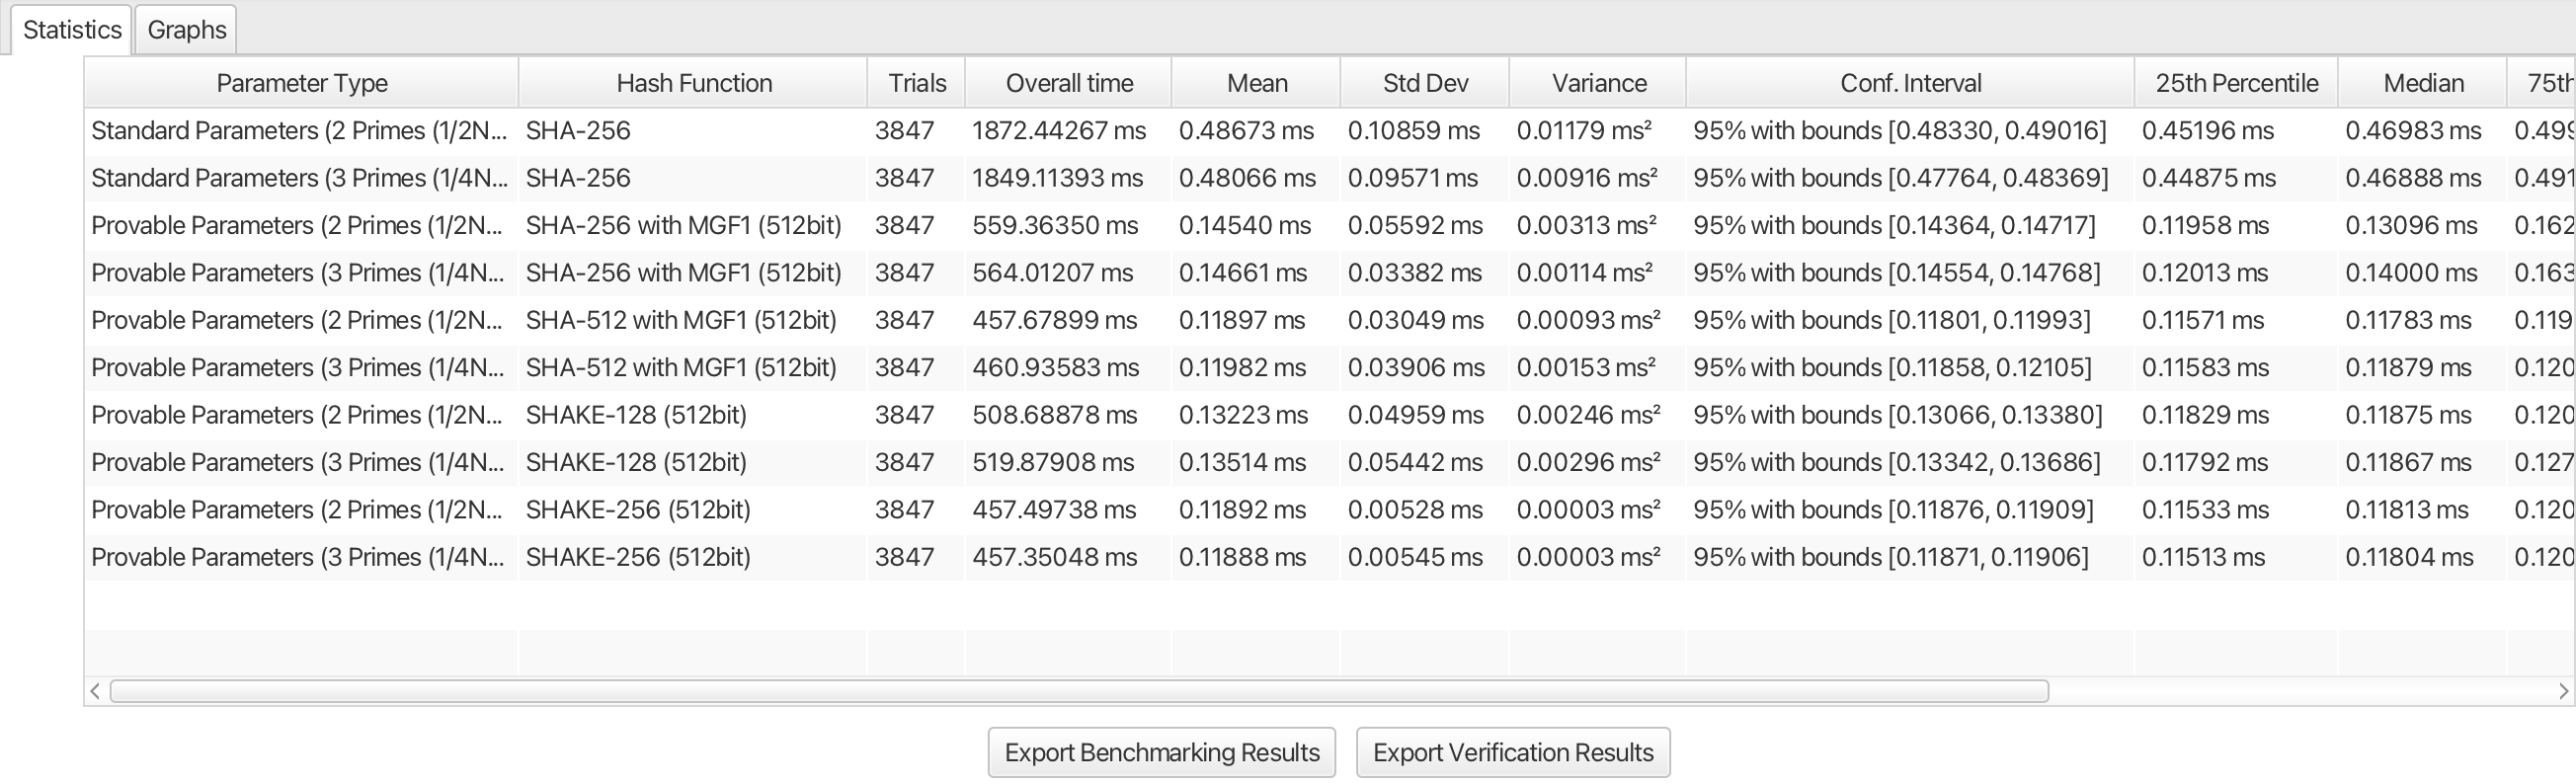
\includegraphics[width=\textwidth]{main_pictures/ansi/ansi_verify_1024bit_table1_1.png}} 
        \fbox{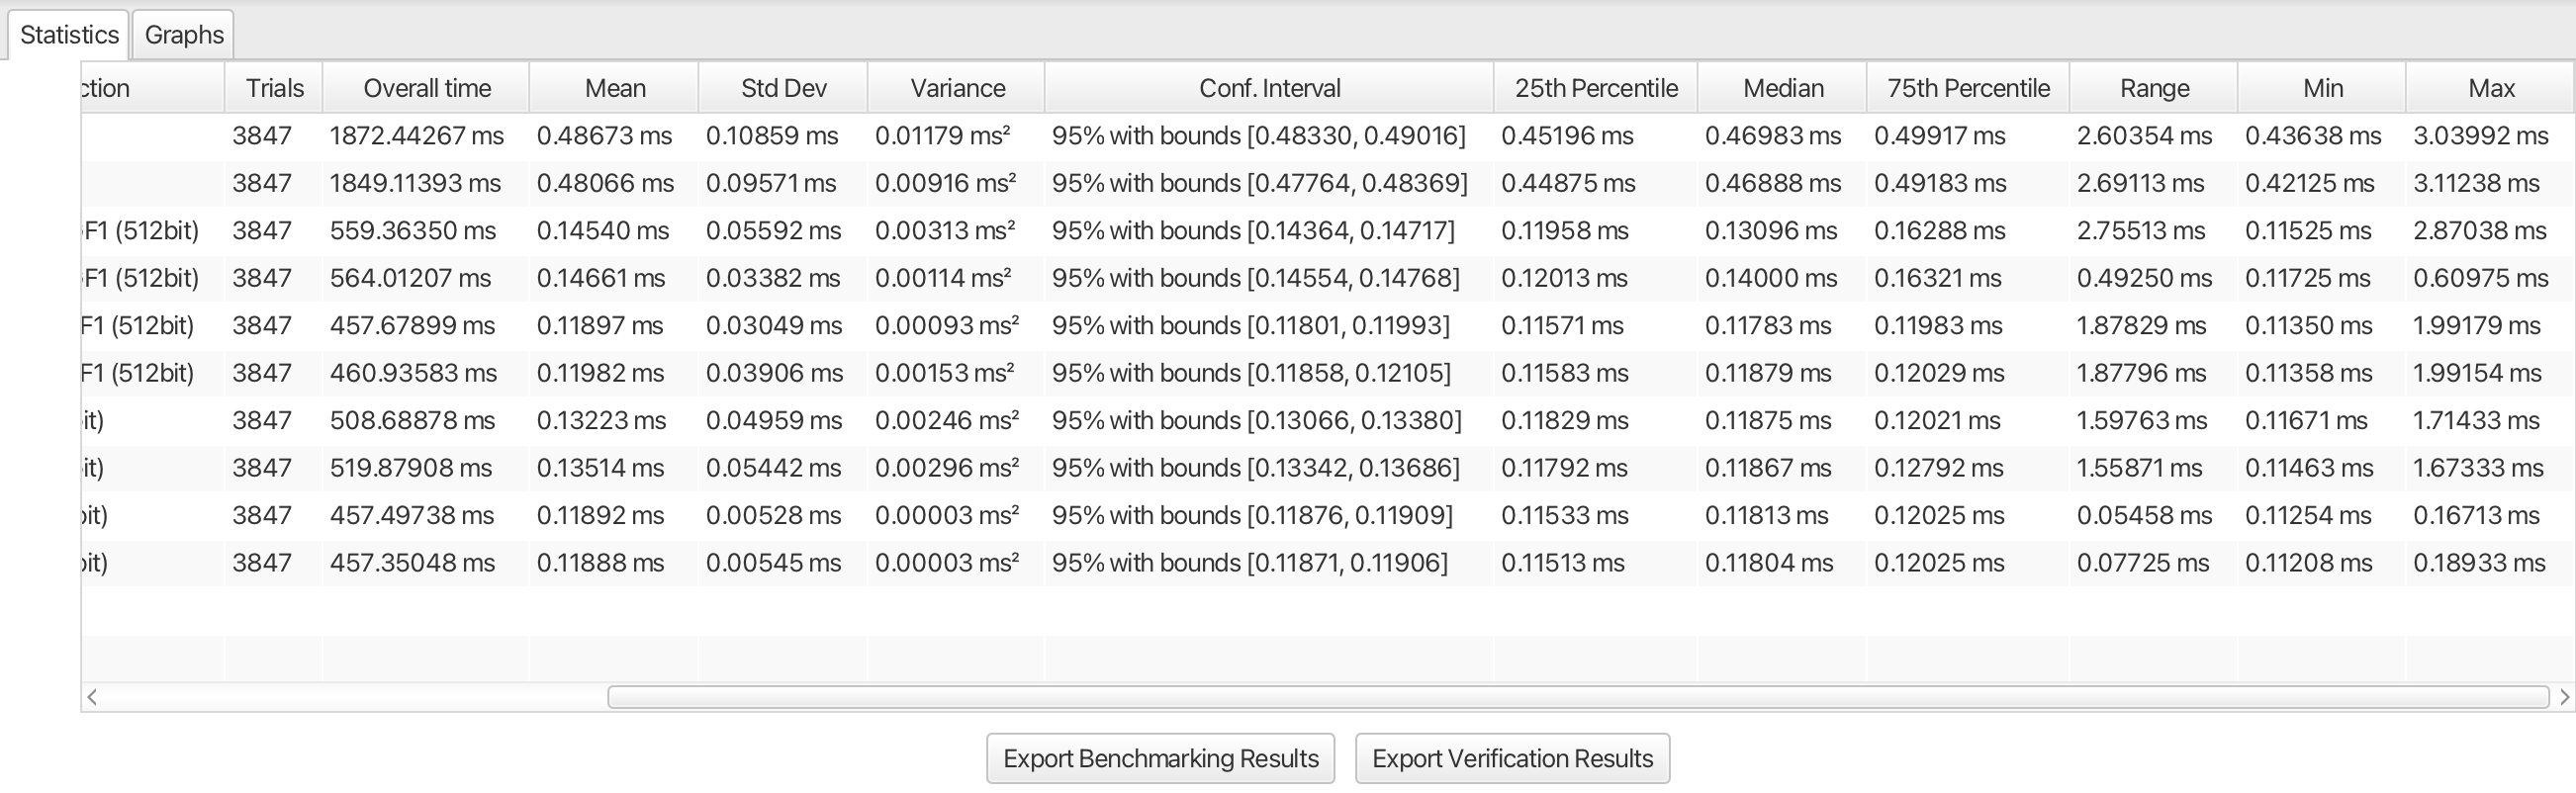
\includegraphics[width=\textwidth]{main_pictures/ansi/ansi_verify_1024bit_table2_1.png}}
    \end{minipage}
       \label{ansi_verify_1024bit_table}
  \end{figure}
  
\begin{figure}[H]
    \centering % Center the images
     \caption{Instantiation of ANSI X9.31 rDSA with standard vs provably secure parameters (2048-bit Key Size) for signature verification}
    % First image in a minipage
    \begin{minipage}{\textwidth}
        \centering
        \fbox{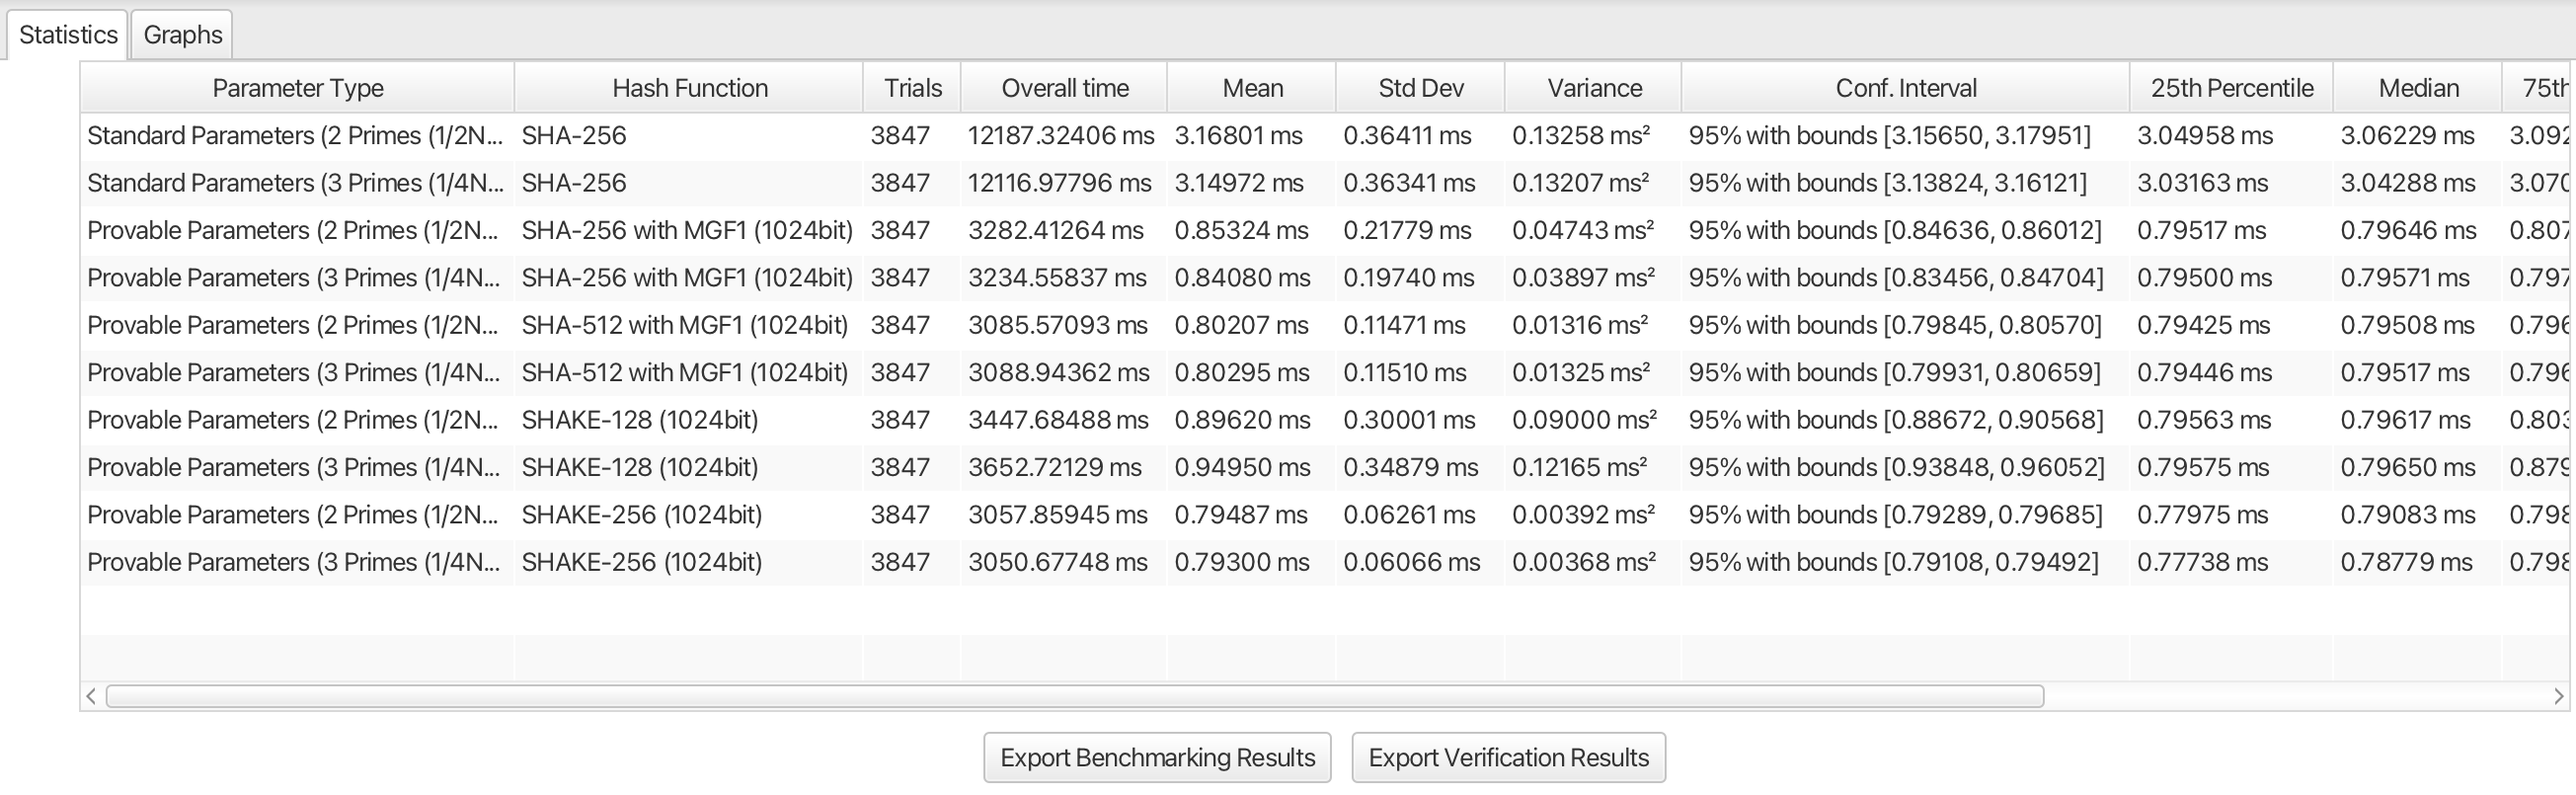
\includegraphics[width=\textwidth]{main_pictures/ansi/ansi_verify_2048bit_table1_1.png}} 
        \fbox{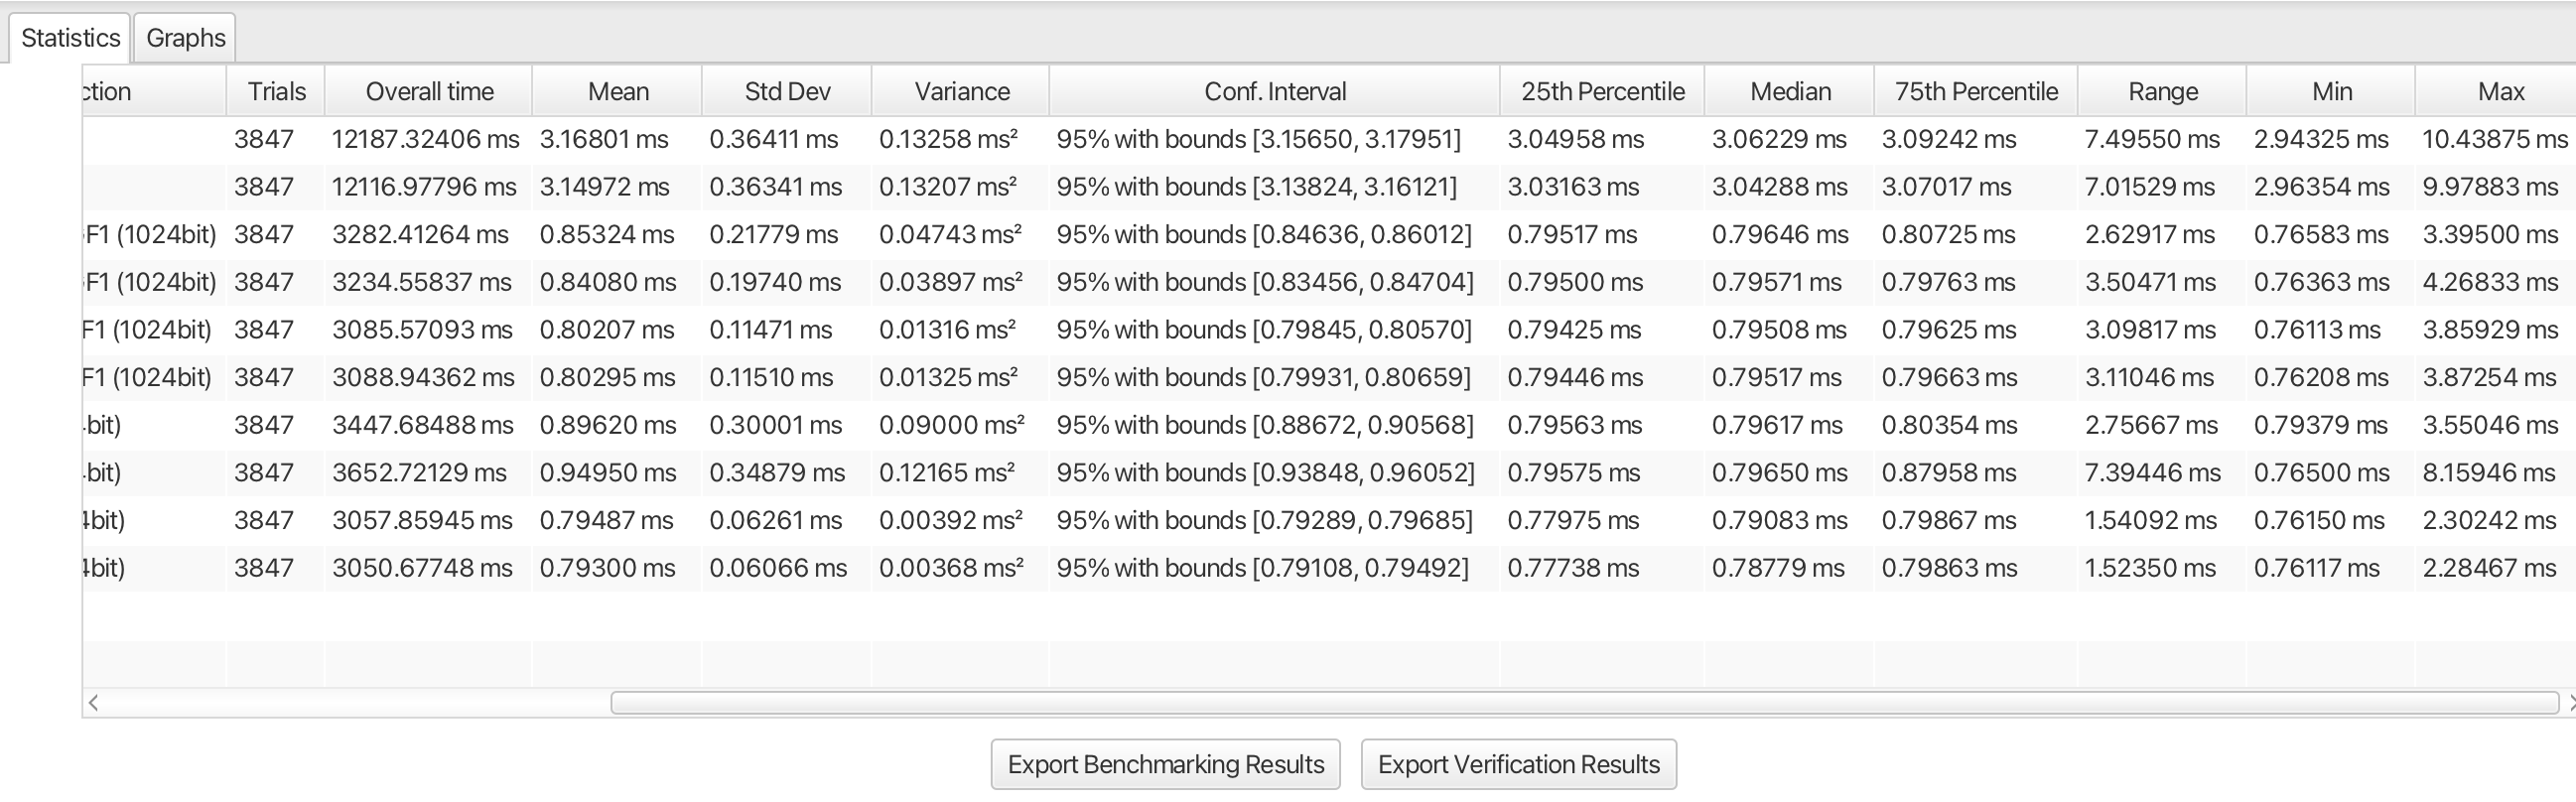
\includegraphics[width=\textwidth]{main_pictures/ansi/ansi_verify_2048bit_table2_1.png}}
    \end{minipage}
           \label{ansi_verify_2048bit_table}
  \end{figure}
  
\begin{figure}[H]
    \centering % Center the images
     \caption{Instantiation of ANSI X9.31 rDSA with standard vs provably secure parameters (3072-bit Key Size) for signature verification}
    % First image in a minipage
    \begin{minipage}{\textwidth}
        \centering
        \fbox{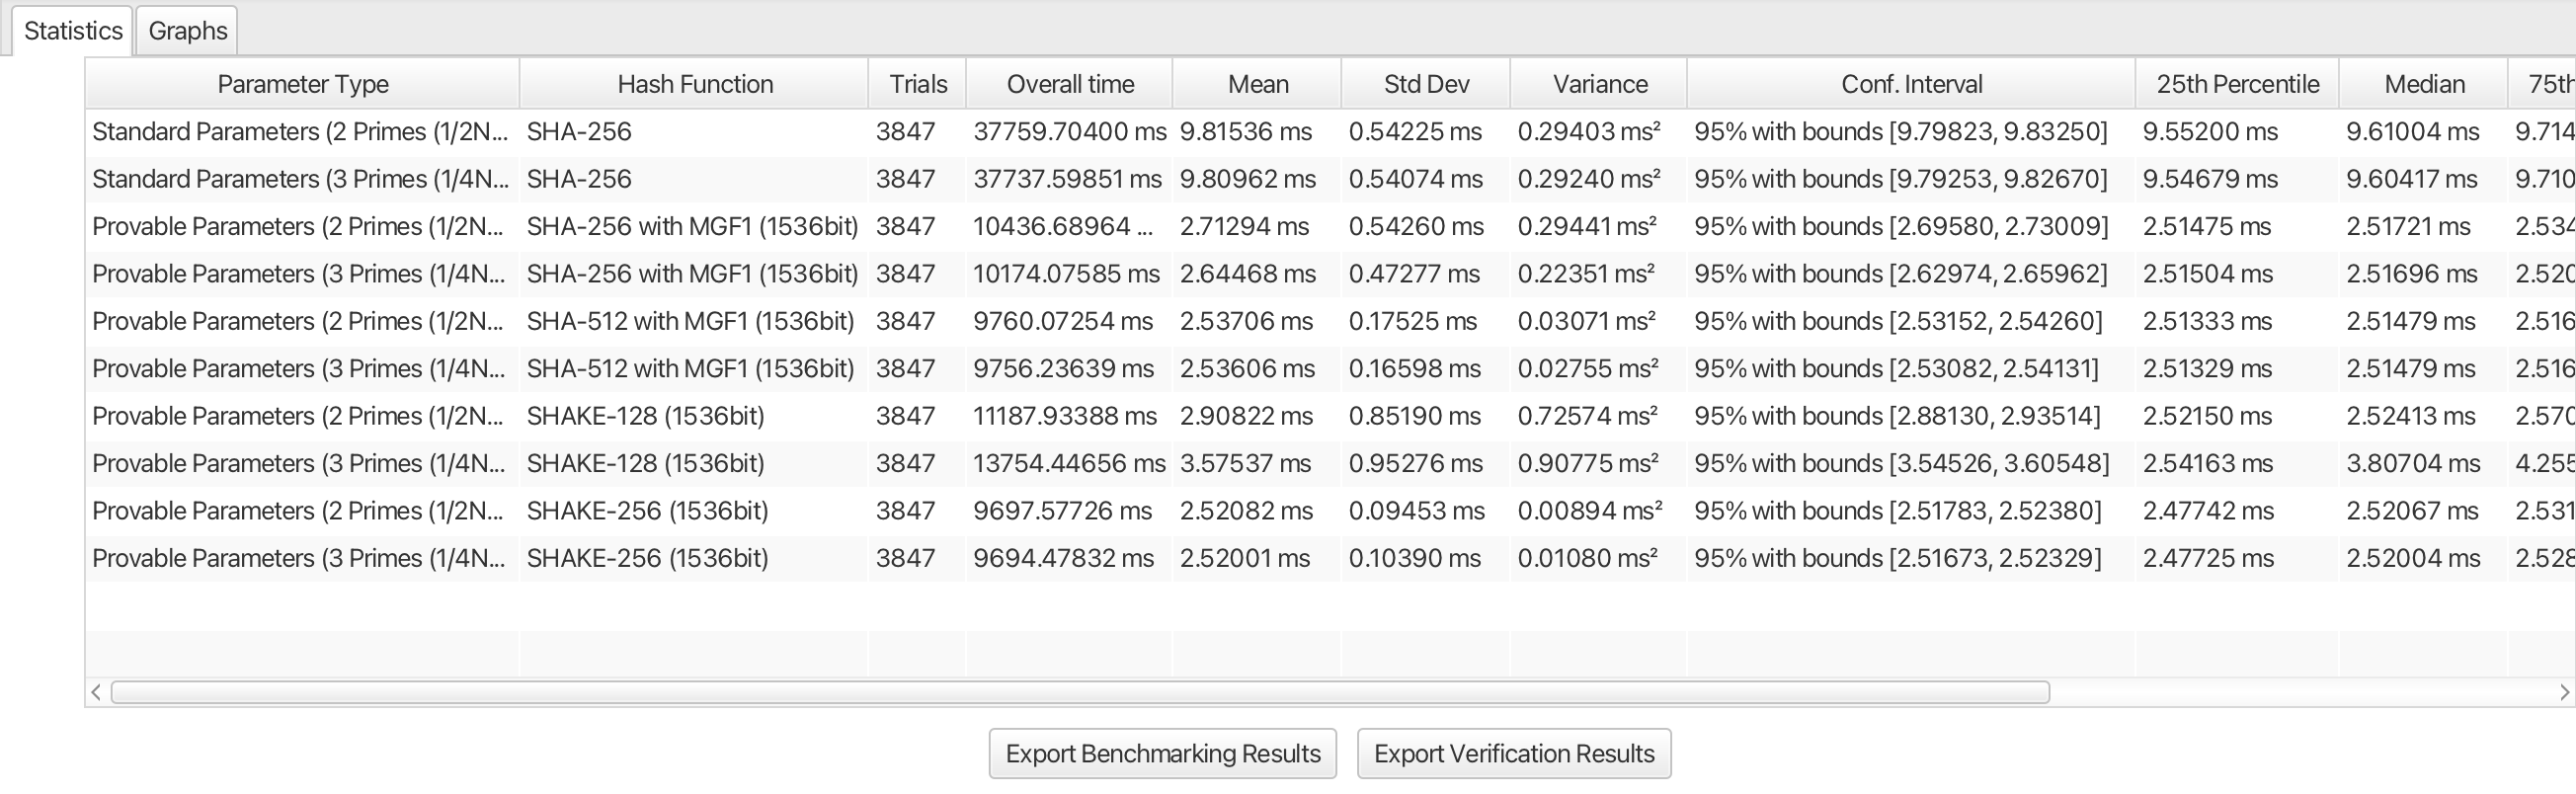
\includegraphics[width=\textwidth]{main_pictures/ansi/ansi_verify_3072bit_table1_1.png}} 
        \fbox{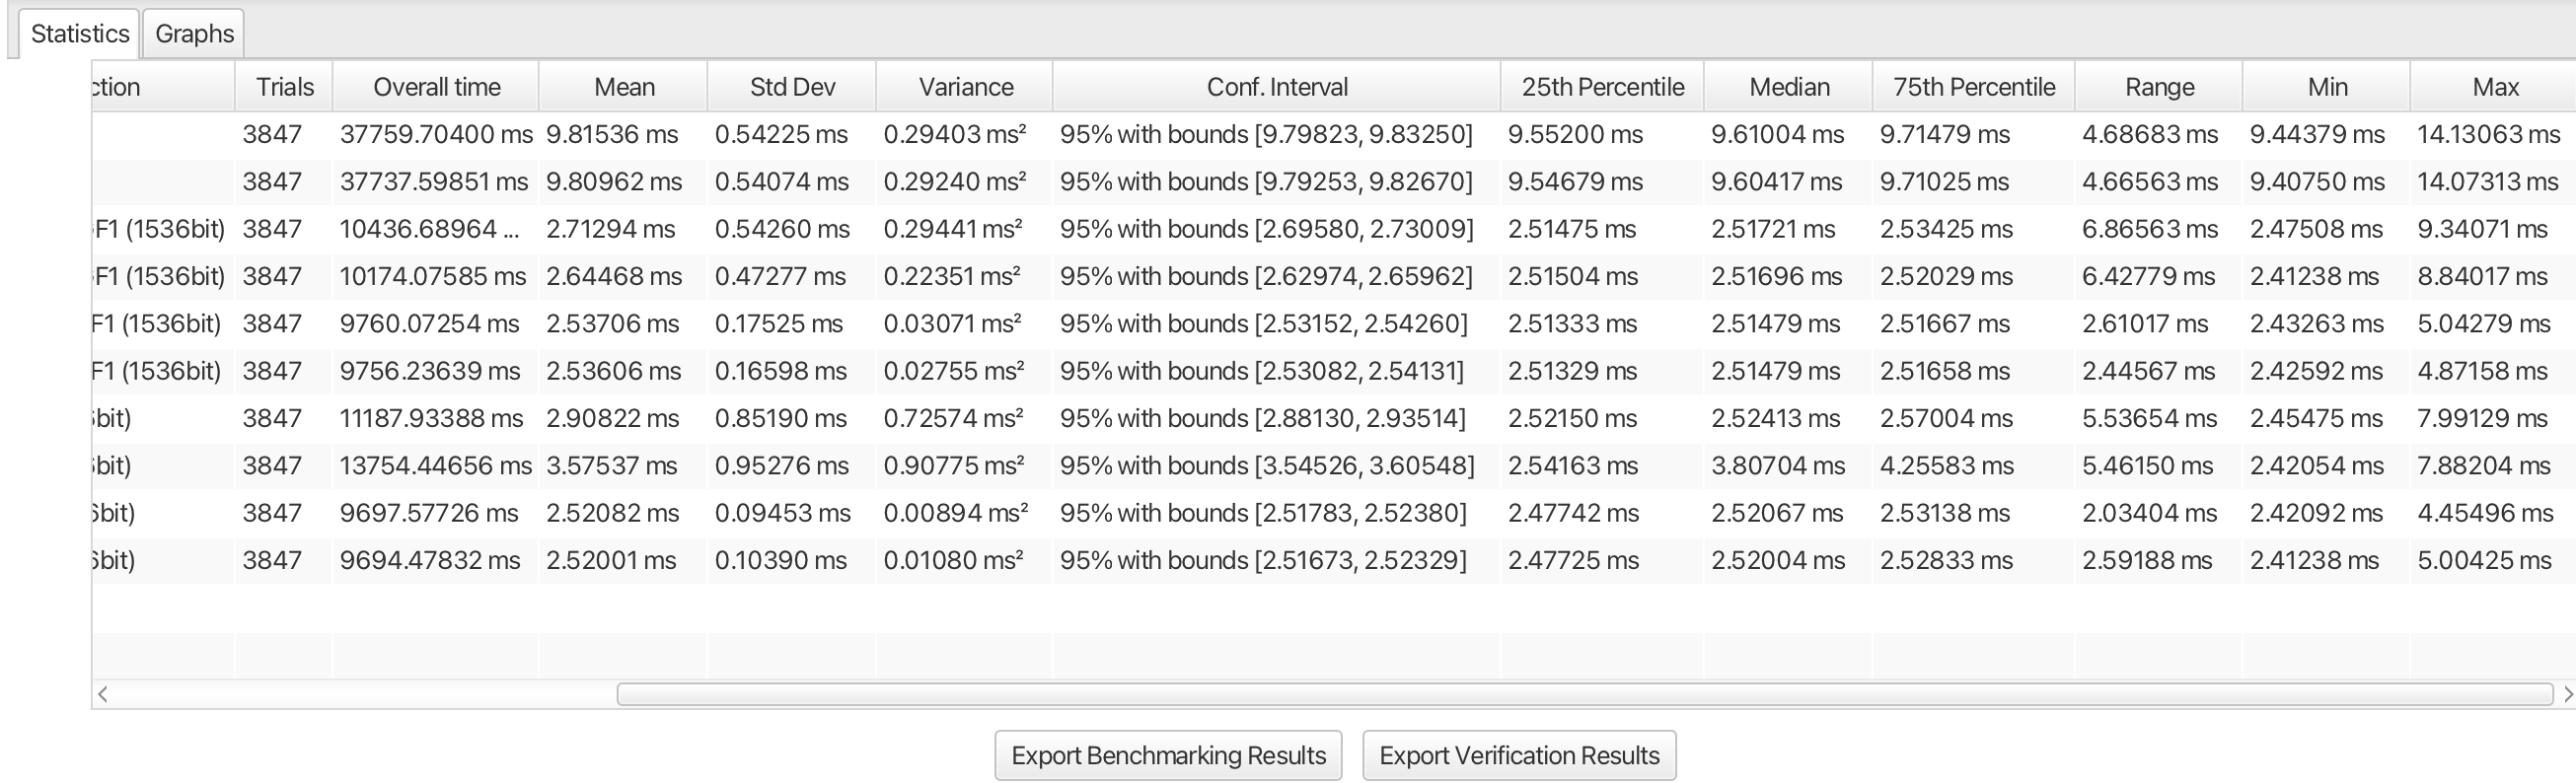
\includegraphics[width=\textwidth]{main_pictures/ansi/ansi_verify_3072bit_table2_1.png}}
    \end{minipage}
          \label{ansi_verify_3072bit_table}
\end{figure}

\begin{figure}[H]
    \centering % Center the images
     \caption{Instantiation of ANSI X9.31 rDSA with standard vs provably secure parameters (4096-bit Key Size) for signature verification}
    % First image in a minipage
    \begin{minipage}{\textwidth}
        \centering
        \fbox{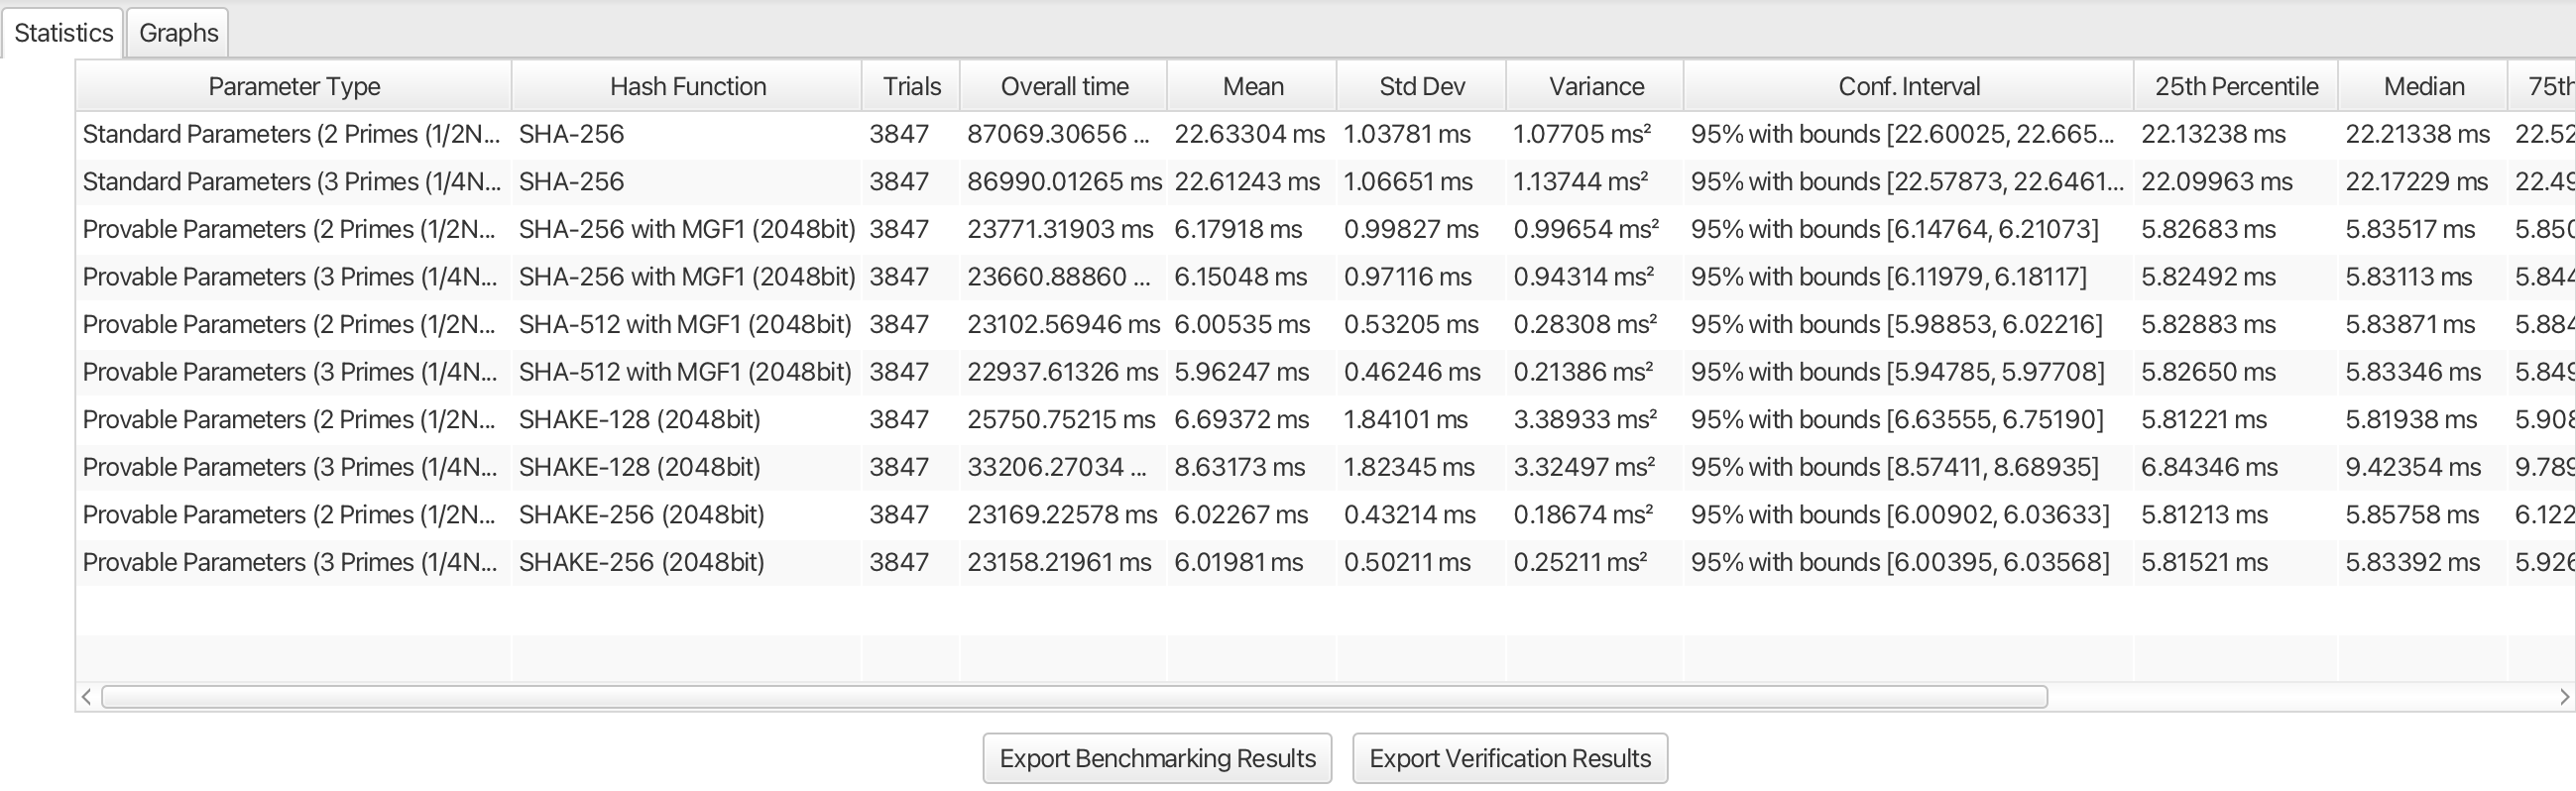
\includegraphics[width=\textwidth]{main_pictures/ansi/ansi_verify_4096bit_table1_1.png}} 
        \fbox{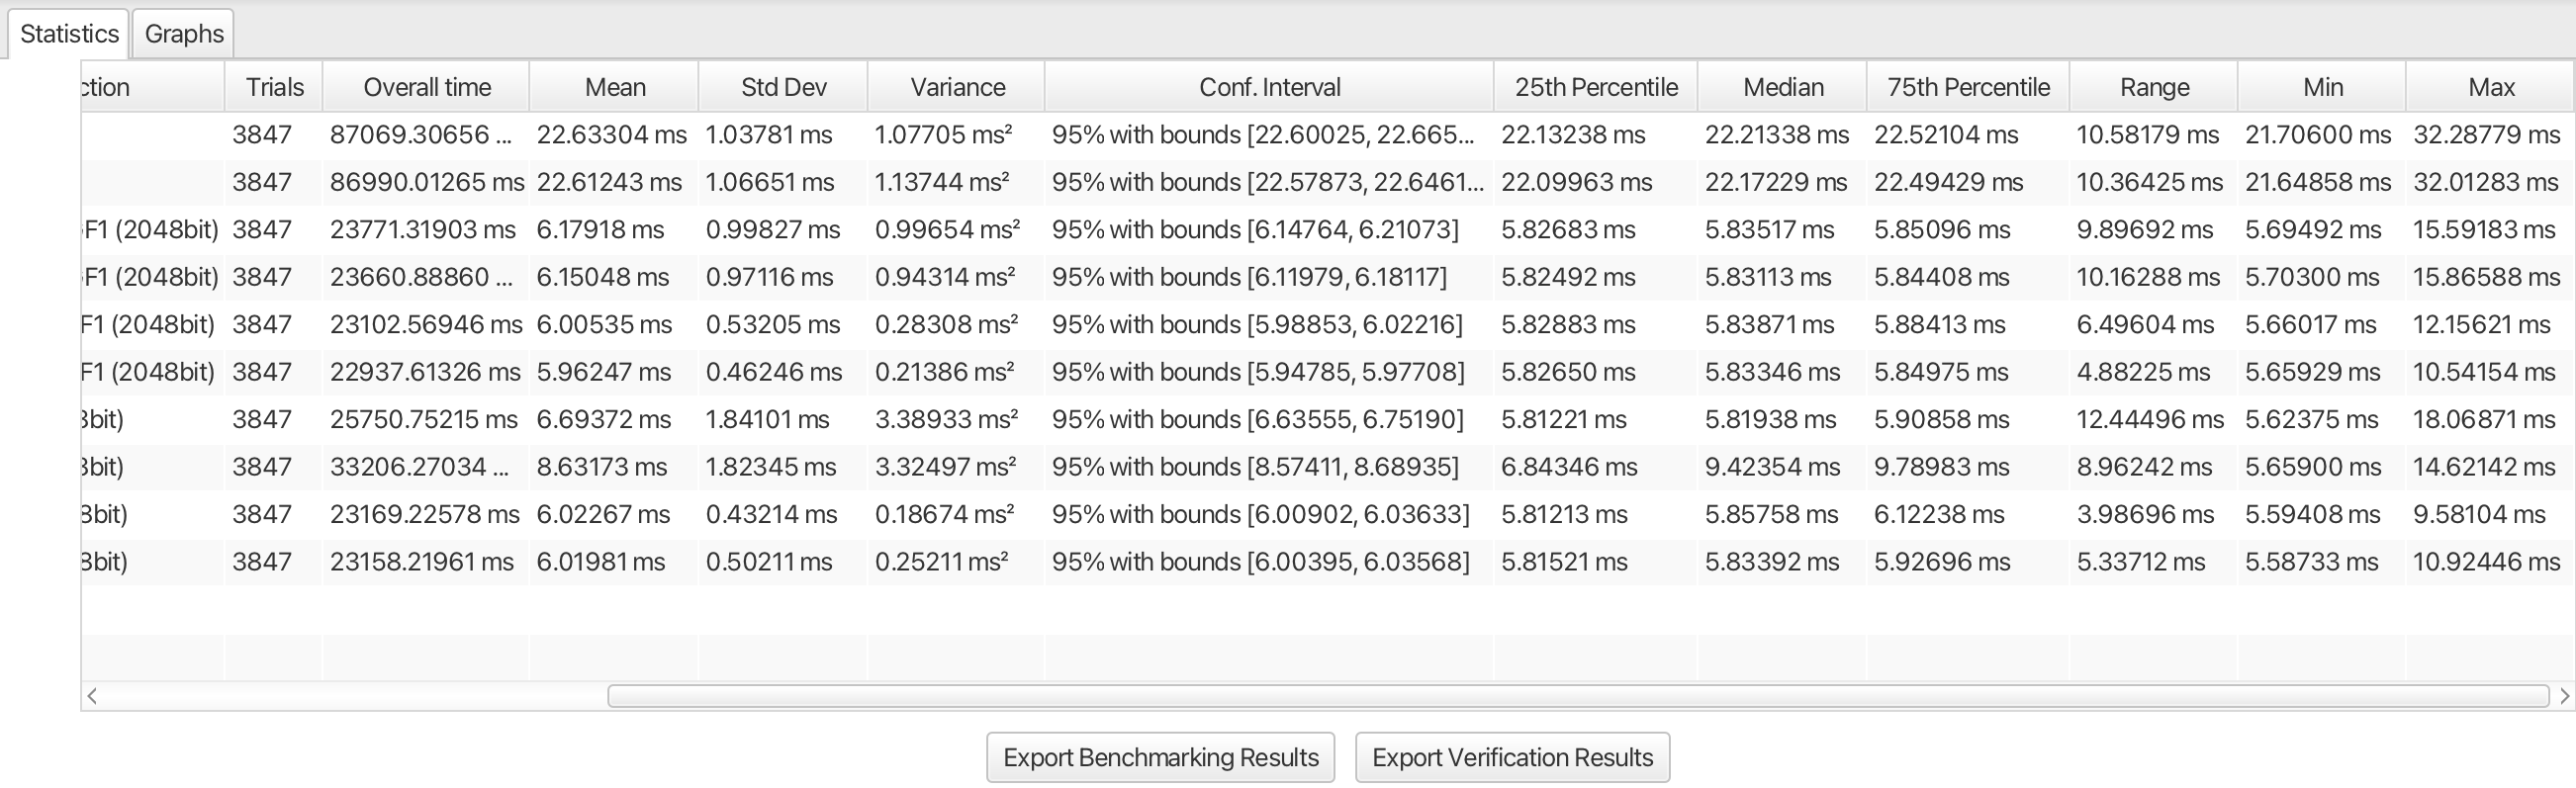
\includegraphics[width=\textwidth]{main_pictures/ansi/ansi_verify_4096bit_table2_1.png}}
    \end{minipage}
         \label{ansi_verify_4096bit_table}
\end{figure}

\begin{figure}[H]
    \centering % Center the images
     \caption{Instantiation of ANSI X9.31 rDSA with standard vs provably secure parameters (5120-bit Key Size) for signature verification}
    % First image in a minipage
    \begin{minipage}{\textwidth}
        \centering
        \fbox{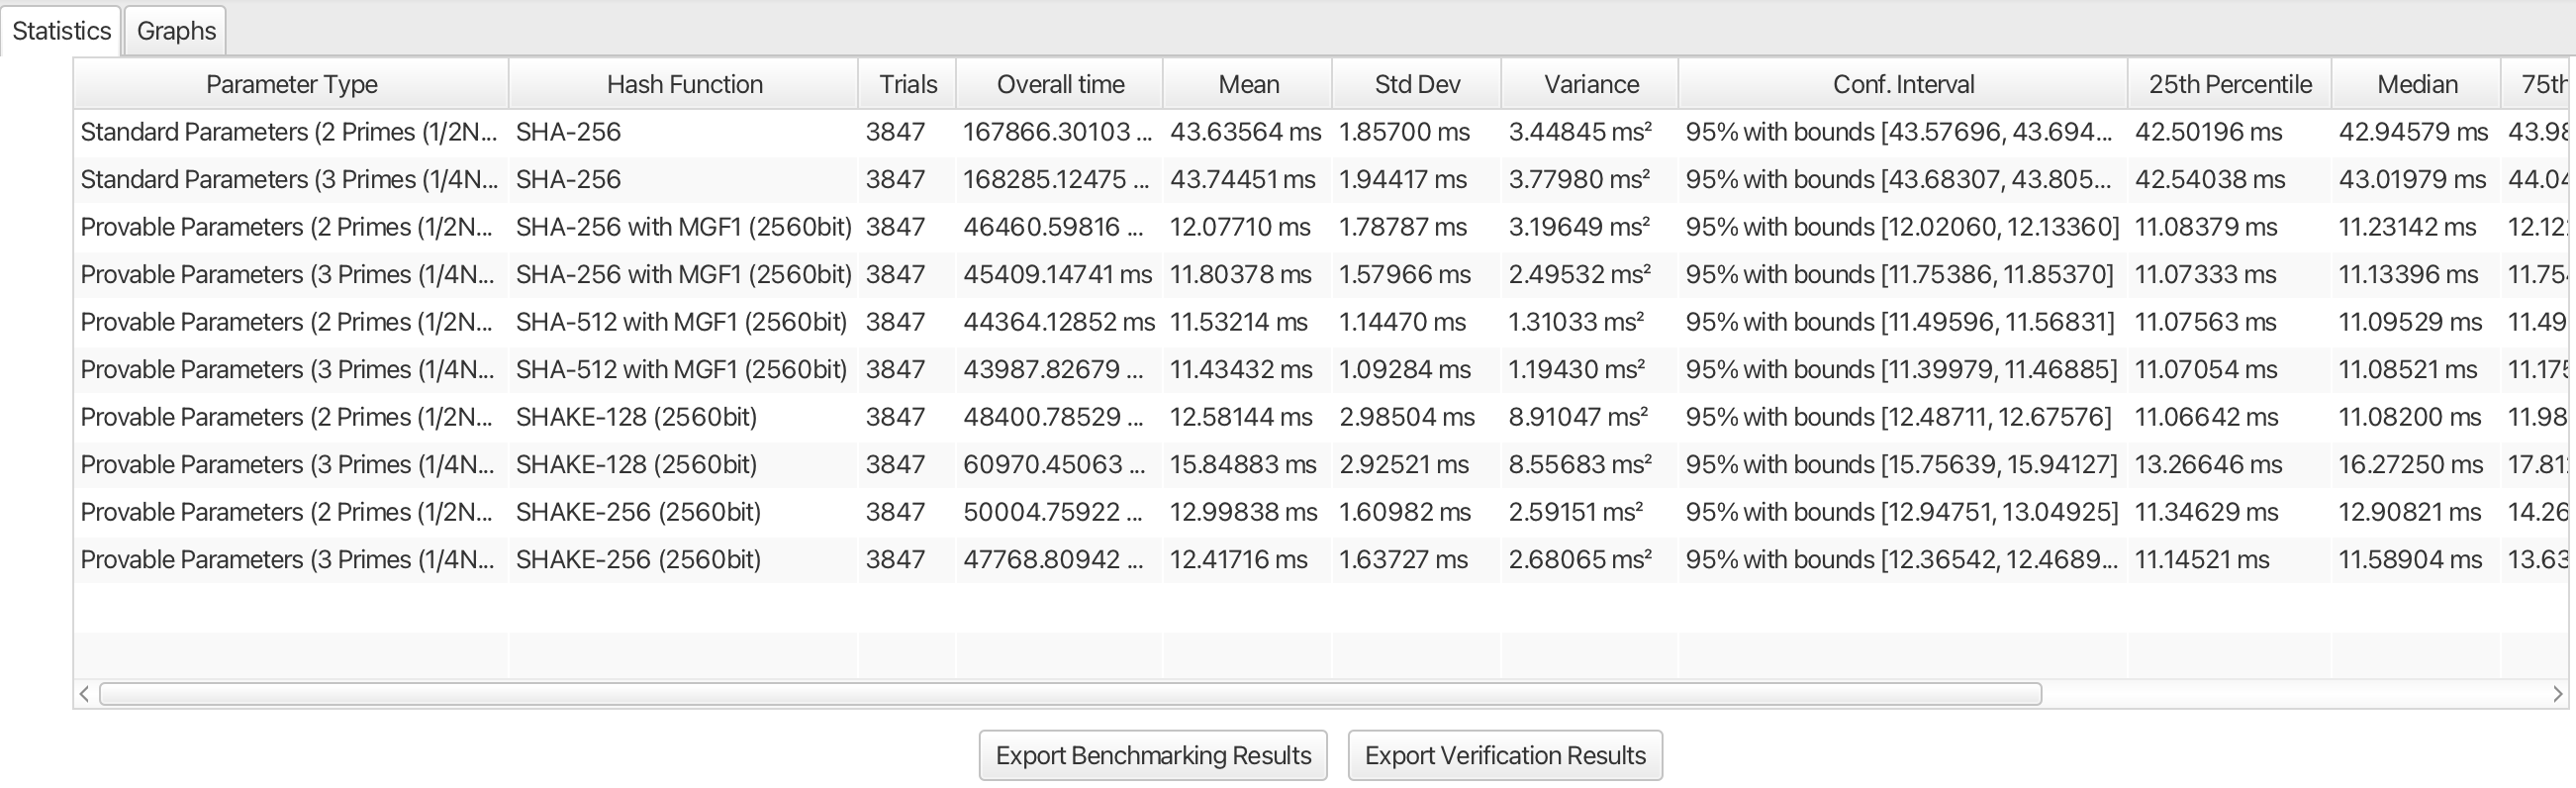
\includegraphics[width=\textwidth]{main_pictures/ansi/ansi_verify_5120bit_table1_1.png}} 
        \fbox{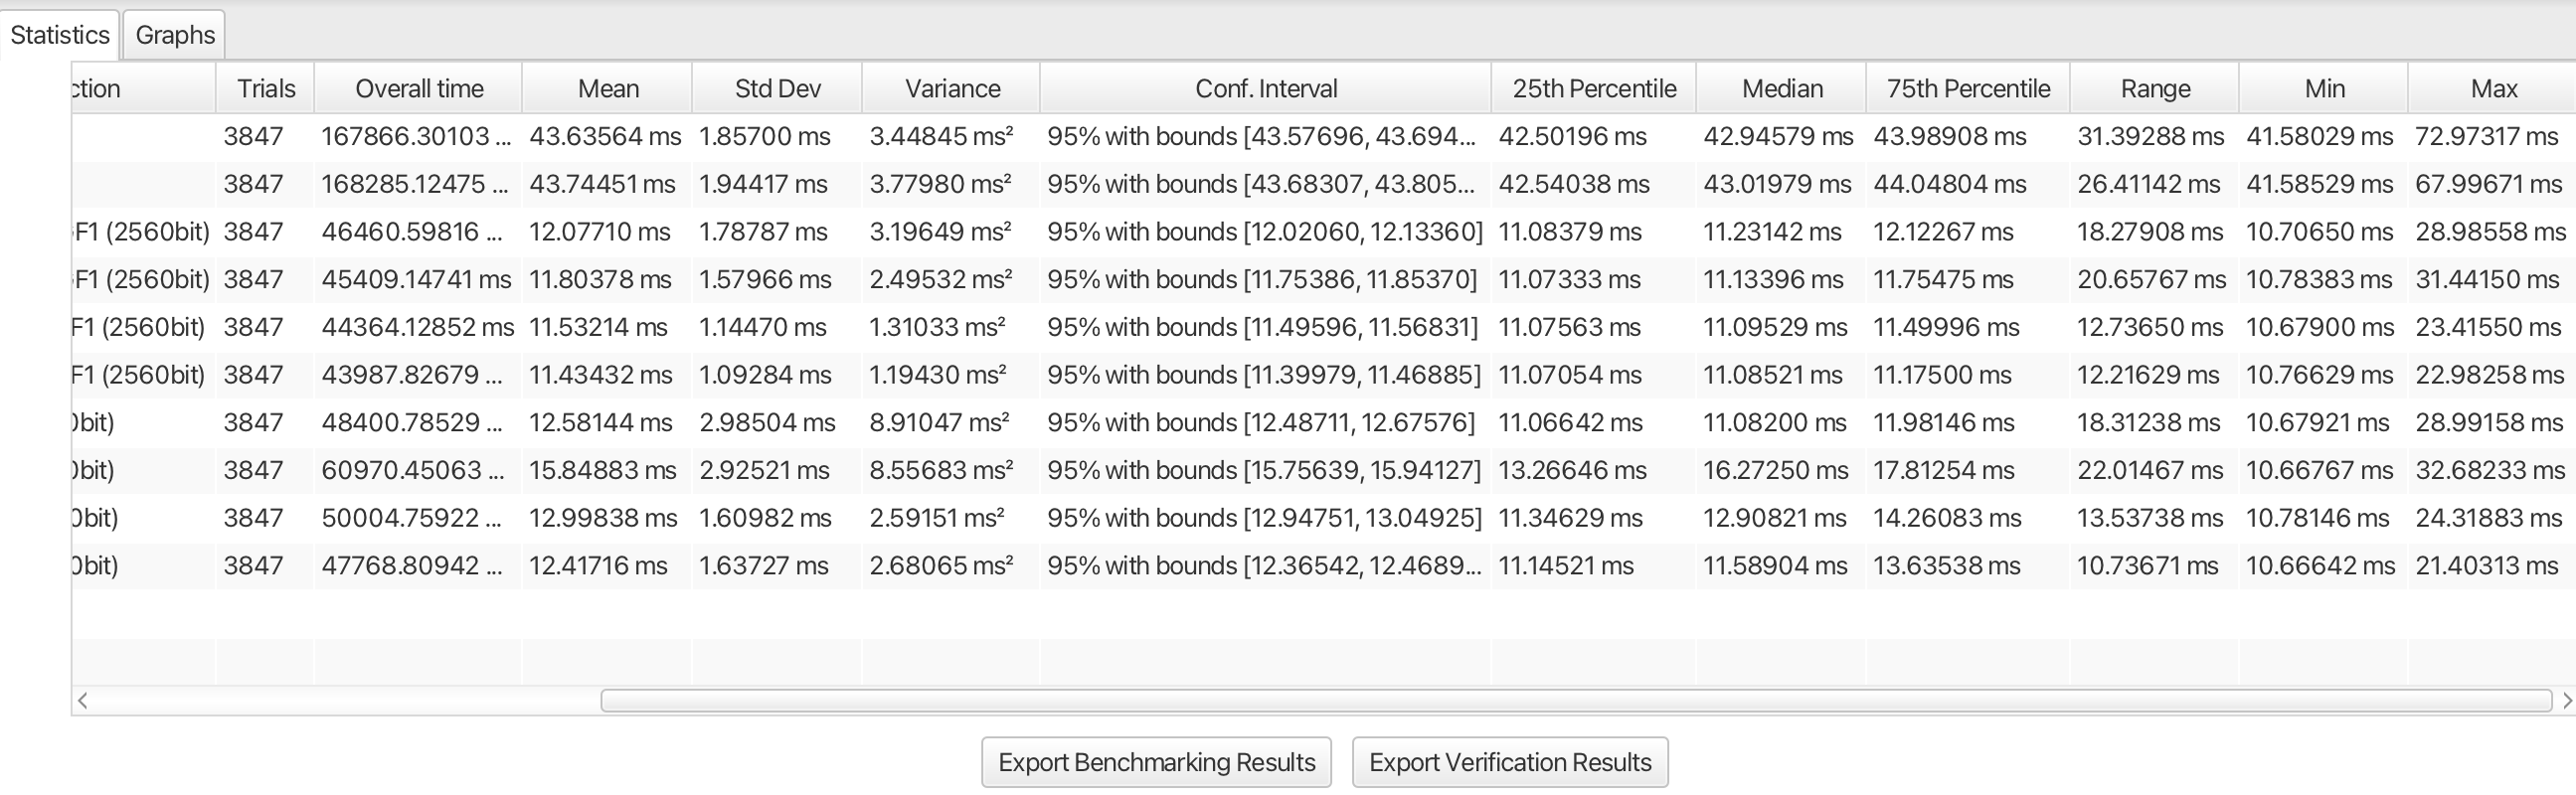
\includegraphics[width=\textwidth]{main_pictures/ansi/ansi_verify_5120bit_table2_1.png}}
    \end{minipage}
       \label{ansi_verify_5120bit_table}
\end{figure}

\begin{figure}[H]
    \centering % Center the images
     \caption{Instantiation of ANSI X9.31 rDSA with standard vs provably secure parameters (6144-bit Key Size) for signature verification}
    % First image in a minipage
    \begin{minipage}{\textwidth}
        \centering
        \fbox{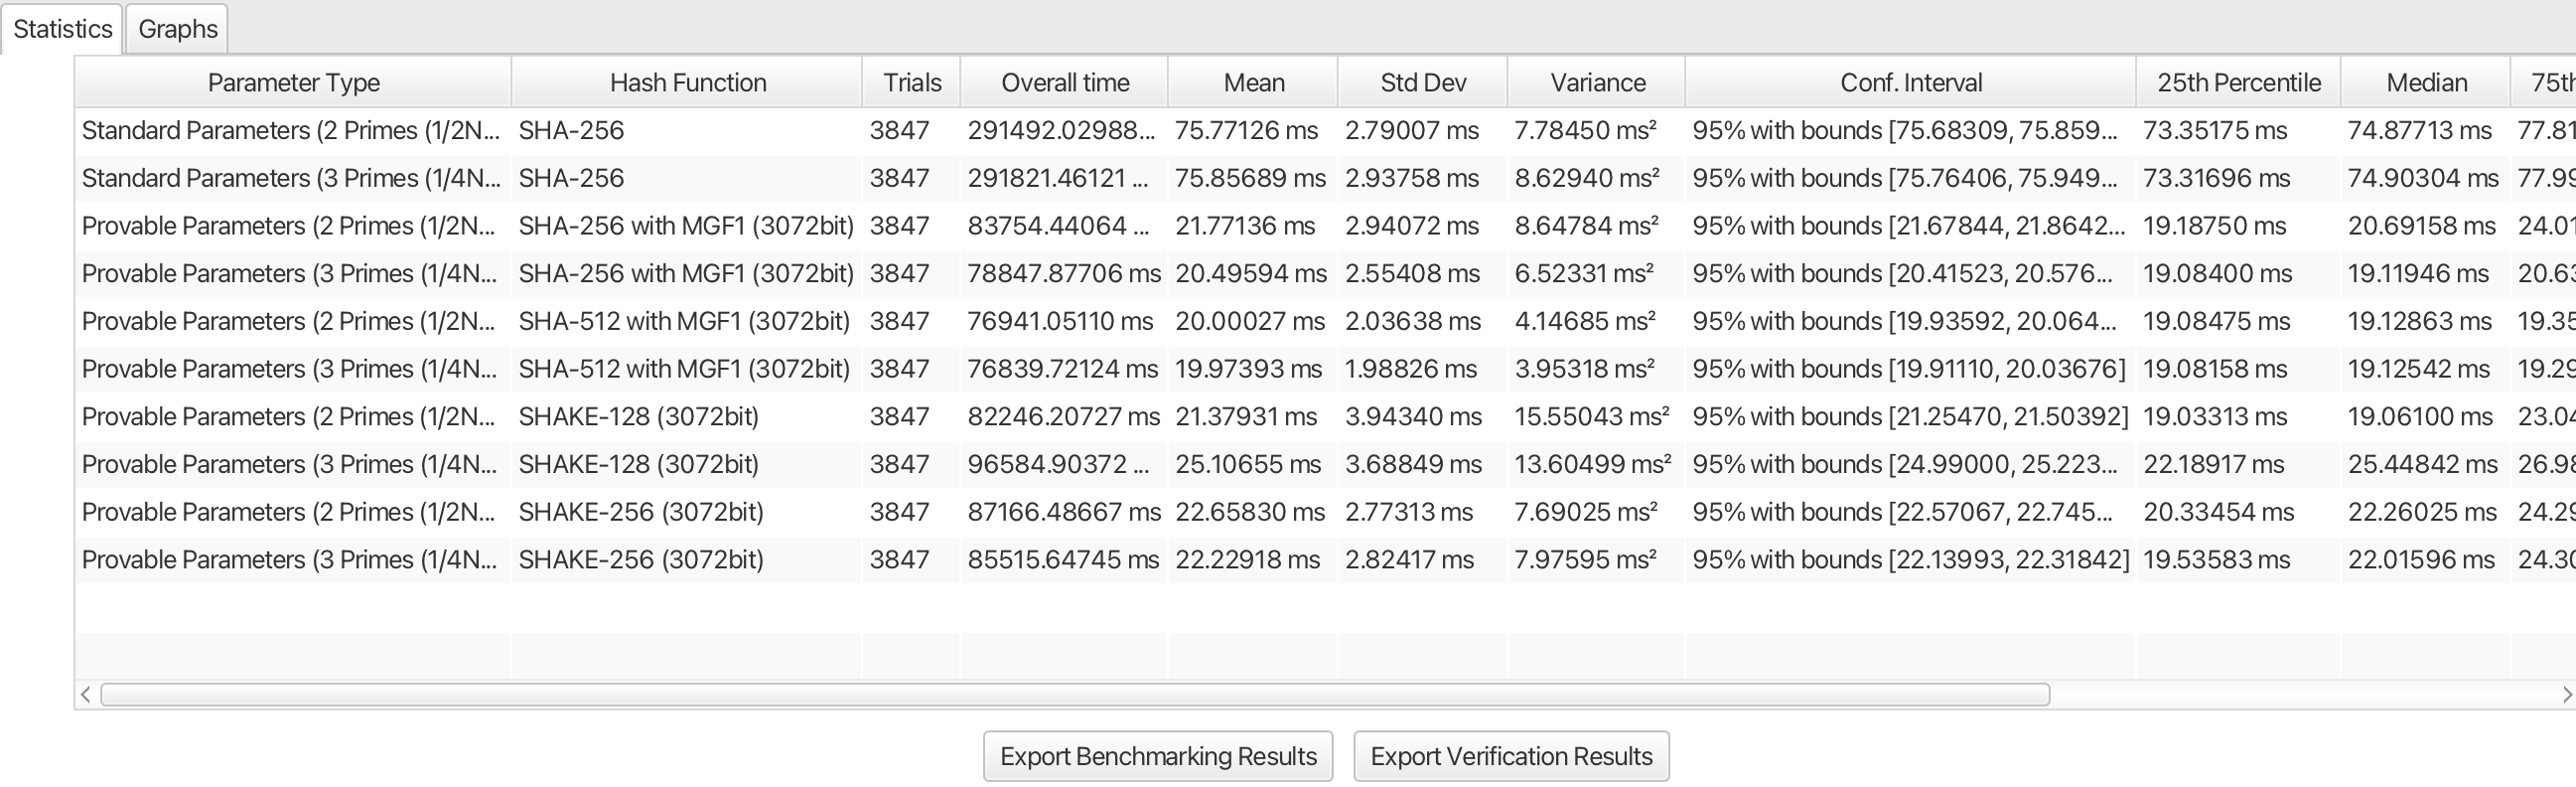
\includegraphics[width=\textwidth]{main_pictures/ansi/ansi_verify_6144bit_table1_1.png}} 
        \fbox{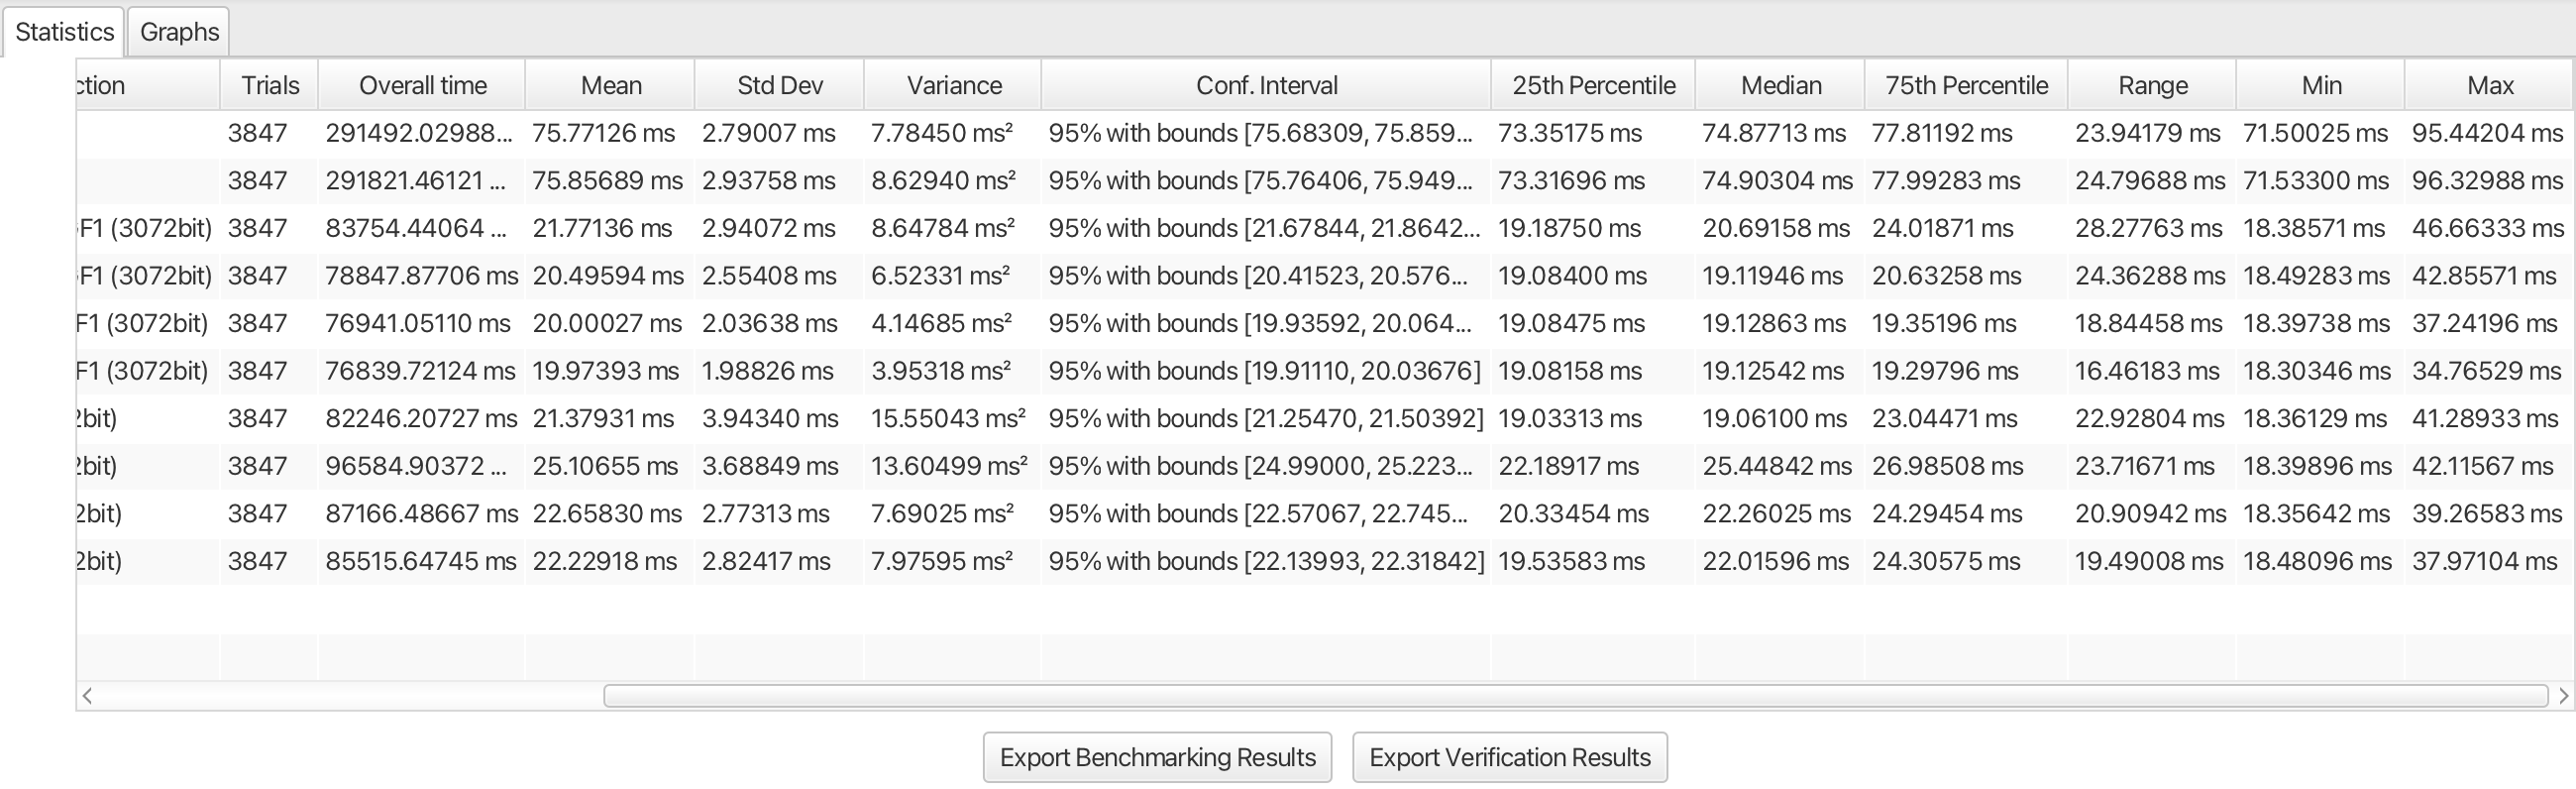
\includegraphics[width=\textwidth]{main_pictures/ansi/ansi_verify_6144bit_table2_1.png}}
    \end{minipage}
         \label{ansi_verify_6144bit_table}
\end{figure}
\end{comment}

\begin{landscape}
\pagestyle{empty}%

\section{Signature Verification Results (ANSI X9.31 rDSA)}

\begin{longtable}{|p{2.3cm}|p{1.8cm}|p{1.0cm}|p{1.7cm}|p{1.4cm}|p{1.5cm}|p{1.8cm}|p{1.5cm}|p{1.43cm}|p{1.5cm}|p{1.3cm}|p{1.4cm}|p{1.3cm}|p{1.3cm}|}

\caption{\textbf{Instantiation of ANSI X9.31 rDSA with Standard vs Provably Secure Parameters (1024-bit Key Size) for Signature Verification}}
     \label{ansi_verify_1024bit_table} \\
\hline
\textbf{Parameter Type} & \textbf{Hash Function} & \textbf{Trials} & \textbf{Overall Time} & \textbf{Mean} & \textbf{Std Dev} & \textbf{Variance} & \textbf{Conf. Interval} & \textbf{25th Percentile} & \textbf{Median} & \textbf{75th Percentile} & \textbf{Range} & \textbf{Min} & \textbf{Max} \\
\hline
\endfirsthead

\multicolumn{14}{c}%
{{\bfseries \tablename\ \thetable{} -- Signature Verification Results for ANSI X9.31 rDSA with 1024-bit Key Size (continued from previous page)}} \\
\hline
\textbf{Parameter Type} & \textbf{Hash Function} & \textbf{Trials} & \textbf{Overall Time} & \textbf{Mean} & \textbf{Std Dev} & \textbf{Variance} & \textbf{Conf. Interval} & \textbf{25th Percentile} & \textbf{Median} & \textbf{75th Percentile} & \textbf{Range} & \textbf{Min} & \textbf{Max} \\
\hline
\endhead

\hline \multicolumn{14}{|r|}{{Continued on next page}} \\ \hline
\endfoot

\hline
\endlastfoot

Standard Parameters (2 Primes) & SHA-256 & 3847 & 1872.
44267 ms & 0.48673 ms & 0.10859 ms & 0.01179 ms\textsuperscript{2} & 95\% with bounds 0.48330 ms - 0.49016 ms & 0.45196 ms & 0.46983 ms & 0.49917 ms & 2.60354 ms & 0.43638 ms & 3.03992 ms \\
\hline
Standard Parameters (3 Primes) & SHA-256 & 3847 & 1849.
11393 ms & 0.48066 ms & 0.09571 ms & 0.00916 ms\textsuperscript{2} & 95\% with bounds 0.47764 ms - 0.48369 ms & 0.44875 ms & 0.46888 ms & 0.49183 ms & 2.69113 ms & 0.42125 ms & 3.11238 ms \\
\hline
Provable Parameters (2 Primes) & SHA-256 with MGF1 (512bit) & 3847 & 559.
36350 ms & 0.14540 ms & 0.05592 ms & 0.00313 ms\textsuperscript{2} & 95\% with bounds 0.14364 ms - 0.14717 ms & 0.11958 ms & 0.13096 ms & 0.16288 ms & 2.75513 ms & 0.11525 ms & 2.87038 ms \\
\hline
Provable Parameters (3 Primes) & SHA-256 with MGF1 (512bit) & 3847 & 564.
01207 ms & 0.14661 ms & 0.03382 ms & 0.00114 ms\textsuperscript{2} & 95\% with bounds 0.14554 ms - 0.14768 ms & 0.12013 ms & 0.14000 ms & 0.16321 ms & 0.49250 ms & 0.11725 ms & 0.60975 ms \\
\hline
Provable Parameters (2 Primes) & SHA-512 with MGF1 (512bit) & 3847 & 457.
67899 ms & 0.11897 ms & 0.03049 ms & 0.00093 ms\textsuperscript{2} & 95\% with bounds 0.11801 ms - 0.11993 ms & 0.11571 ms & 0.11783 ms & 0.11983 ms & 1.87829 ms & 0.11350 ms & 1.99179 ms \\
\hline
Provable Parameters (3 Primes) & SHA-512 with MGF1 (512bit) & 3847 & 460.
93583 ms & 0.11982 ms & 0.03906 ms & 0.00153 ms\textsuperscript{2} & 95\% with bounds 0.11858 ms - 0.12105 ms & 0.11583 ms & 0.11879 ms & 0.12029 ms & 1.87796 ms & 0.11358 ms & 1.99154 ms \\
\hline
Provable Parameters (2 Primes) & SHAKE-128 (512bit) & 3847 & 508.
68878 ms & 0.13223 ms & 0.04959 ms & 0.00246 ms\textsuperscript{2} & 95\% with bounds 0.13066 ms - 0.13380 ms & 0.11829 ms & 0.11875 ms & 0.12021 ms & 1.59763 ms & 0.11671 ms & 1.71433 ms \\
\hline
Provable Parameters (3 Primes) & SHAKE-128 (512bit) & 3847 & 519.
87908 ms & 0.13514 ms & 0.05442 ms & 0.00296 ms\textsuperscript{2} & 95\% with bounds 0.13342 ms - 0.13686 ms & 0.11792 ms & 0.11867 ms & 0.12792 ms & 1.55871 ms & 0.11463 ms & 1.67333 ms \\
\hline
Provable Parameters (2 Primes) & SHAKE-256 (512bit) & 3847 & 457.
49738 ms & 0.11892 ms & 0.00528 ms & 0.00003 ms\textsuperscript{2} & 95\% with bounds 0.11876 ms - 0.11909 ms & 0.11533 ms & 0.11813 ms & 0.12025 ms & 0.05458 ms & 0.11254 ms & 0.16713 ms \\
\hline
Provable Parameters (3 Primes) & SHAKE-256 (512bit) & 3847 & 457.
35048 ms & 0.11888 ms & 0.00545 ms & 0.00003 ms\textsuperscript{2} & 95\% with bounds 0.11871 ms - 0.11906 ms & 0.11513 ms & 0.11804 ms & 0.12025 ms & 0.07725 ms & 0.11208 ms & 0.18933 ms \\
\hline

\end{longtable}

\begin{longtable}{|p{2.3cm}|p{1.8cm}|p{1.0cm}|p{1.7cm}|p{1.4cm}|p{1.5cm}|p{1.8cm}|p{1.5cm}|p{1.43cm}|p{1.5cm}|p{1.3cm}|p{1.4cm}|p{1.3cm}|p{1.3cm}|}

\caption{\textbf{Instantiation of ANSI X9.31 rDSA with Standard vs Provably Secure Parameters (2048-bit Key Size) for Signature Verification}}
     \label{ansi_verify_2048bit_table} \\
\hline
\textbf{Parameter Type} & \textbf{Hash Function} & \textbf{Trials} & \textbf{Overall Time} & \textbf{Mean} & \textbf{Std Dev} & \textbf{Variance} & \textbf{Conf. Interval} & \textbf{25th Percentile} & \textbf{Median} & \textbf{75th Percentile} & \textbf{Range} & \textbf{Min} & \textbf{Max} \\
\hline
\endfirsthead

\multicolumn{14}{c}%
{{\bfseries \tablename\ \thetable{} -- Signature Verification Results for ANSI X9.31 rDSA with 2048-bit Key Size (continued from previous page)}} \\
\hline
\textbf{Parameter Type} & \textbf{Hash Function} & \textbf{Trials} & \textbf{Overall Time} & \textbf{Mean} & \textbf{Std Dev} & \textbf{Variance} & \textbf{Conf. Interval} & \textbf{25th Percentile} & \textbf{Median} & \textbf{75th Percentile} & \textbf{Range} & \textbf{Min} & \textbf{Max} \\
\hline
\endhead

\hline \multicolumn{14}{|r|}{{Continued on next page}} \\ \hline
\endfoot

\hline
\endlastfoot
Standard Parameters (2 Primes) & SHA-256 & 3847 & 12187.
32406 ms & 3.16801 ms & 0.36411 ms & 0.13258 ms\textsuperscript{2} & 95\% with bounds 3.15650 ms - 3.17951 ms & 3.04958 ms & 3.06229 ms & 3.09242 ms & 7.49550 ms & 2.94325 ms & 10.43875 ms \\
\hline
Standard Parameters (3 Primes) & SHA-256 & 3847 & 12116.
97796 ms & 3.14972 ms & 0.36341 ms & 0.13207 ms\textsuperscript{2} & 95\% with bounds 3.13824 ms - 3.16121 ms & 3.03163 ms & 3.04288 ms & 3.07017 ms & 7.01529 ms & 2.96354 ms & 9.97883 ms \\
\hline
Provable Parameters (2 Primes) & SHA-256 with MGF1 (1024bit) & 3847 & 3282.
41264 ms & 0.85324 ms & 0.21779 ms & 0.04743 ms\textsuperscript{2} & 95\% with bounds 0.84636 ms - 0.86012 ms & 0.79517 ms & 0.79646 ms & 0.80725 ms & 2.62917 ms & 0.76583 ms & 3.39500 ms \\
\hline
Provable Parameters (3 Primes) & SHA-256 with MGF1 (1024bit) & 3847 & 3234.
55837 ms & 0.84080 ms & 0.19740 ms & 0.03897 ms\textsuperscript{2} & 95\% with bounds 0.83456 ms - 0.84704 ms & 0.79500 ms & 0.79571 ms & 0.79763 ms & 3.50471 ms & 0.76363 ms & 4.26833 ms \\
\hline
Provable Parameters (2 Primes) & SHA-512 with MGF1 (1024bit) & 3847 & 3085.
57093 ms & 0.80207 ms & 0.11471 ms & 0.01316 ms\textsuperscript{2} & 95\% with bounds 0.79845 ms - 0.80570 ms & 0.79425 ms & 0.79508 ms & 0.79625 ms & 3.09817 ms & 0.76113 ms & 3.85929 ms \\
\hline
Provable Parameters (3 Primes) & SHA-512 with MGF1 (1024bit) & 3847 & 3088.
94362 ms & 0.80295 ms & 0.11510 ms & 0.01325 ms\textsuperscript{2} & 95\% with bounds 0.79931 ms - 0.80659 ms & 0.79446 ms & 0.79517 ms & 0.79663 ms & 3.11046 ms & 0.76208 ms & 3.87254 ms \\
\hline
Provable Parameters (2 Primes) & SHAKE-128 (1024bit) & 3847 & 3447.
68488 ms & 0.89620 ms & 0.30001 ms & 0.09000 ms\textsuperscript{2} & 95\% with bounds 0.88672 ms - 0.90568 ms & 0.79563 ms & 0.79617 ms & 0.80354 ms & 2.75667 ms & 0.79379 ms & 3.55046 ms \\
\hline
Provable Parameters (3 Primes) & SHAKE-128 (1024bit) & 3847 & 3652.
72129 ms & 0.94950 ms & 0.34879 ms & 0.12165 ms\textsuperscript{2} & 95\% with bounds 0.93848 ms - 0.96052 ms & 0.79575 ms & 0.79650 ms & 0.87958 ms & 7.39446 ms & 0.76500 ms & 8.15946 ms \\
\hline
Provable Parameters (2 Primes) & SHAKE-256 (1024bit) & 3847 & 3057.
85945 ms & 0.79487 ms & 0.06261 ms & 0.00392 ms\textsuperscript{2} & 95\% with bounds 0.79289 ms - 0.79685 ms & 0.77975 ms & 0.79083 ms & 0.79867 ms & 1.54092 ms & 0.76150 ms & 2.30242 ms \\
\hline
Provable Parameters (3 Primes) & SHAKE-256 (1024bit) & 3847 & 3050.
67748 ms & 0.79300 ms & 0.06066 ms & 0.00368 ms\textsuperscript{2} & 95\% with bounds 0.79108 ms - 0.79492 ms & 0.77738 ms & 0.78779 ms & 0.79863 ms & 1.52350 ms & 0.76117 ms & 2.28467 ms \\
\hline



\end{longtable}


\begin{longtable}{|p{2.3cm}|p{1.8cm}|p{1.0cm}|p{1.7cm}|p{1.4cm}|p{1.5cm}|p{1.8cm}|p{1.5cm}|p{1.43cm}|p{1.5cm}|p{1.3cm}|p{1.4cm}|p{1.3cm}|p{1.3cm}|}

\caption{\textbf{Instantiation of ANSI X9.31 rDSA with Standard vs Provably Secure Parameters (3072-bit Key Size) for Signature Verification}}
     \label{ansi_verify_3072bit_table} \\
\hline
\textbf{Parameter Type} & \textbf{Hash Function} & \textbf{Trials} & \textbf{Overall Time} & \textbf{Mean} & \textbf{Std Dev} & \textbf{Variance} & \textbf{Conf. Interval} & \textbf{25th Percentile} & \textbf{Median} & \textbf{75th Percentile} & \textbf{Range} & \textbf{Min} & \textbf{Max} \\
\hline
\endfirsthead

\multicolumn{14}{c}%
{{\bfseries \tablename\ \thetable{} -- Signature Verification Results for ANSI X9.31 rDSA with 3072-bit Key Size (continued from previous page)}} \\
\hline
\textbf{Parameter Type} & \textbf{Hash Function} & \textbf{Trials} & \textbf{Overall Time} & \textbf{Mean} & \textbf{Std Dev} & \textbf{Variance} & \textbf{Conf. Interval} & \textbf{25th Percentile} & \textbf{Median} & \textbf{75th Percentile} & \textbf{Range} & \textbf{Min} & \textbf{Max} \\
\hline
\endhead

\hline \multicolumn{14}{|r|}{{Continued on next page}} \\ \hline
\endfoot

\hline
\endlastfoot
Standard Parameters (2 Primes) & SHA-256 & 3847 & 37759.
70400 ms & 9.81536 ms & 0.54225 ms & 0.29403 ms\textsuperscript{2} & 95\% with bounds 9.79823 ms - 9.83250 ms & 9.55200 ms & 9.61004 ms & 9.71479 ms & 4.68683 ms & 9.44379 ms & 14.13063 ms \\
\hline
Standard Parameters (3 Primes) & SHA-256 & 3847 & 37737.
59851 ms & 9.80962 ms & 0.54074 ms & 0.29240 ms\textsuperscript{2} & 95\% with bounds 9.79253 ms - 9.82670 ms & 9.54679 ms & 9.60417 ms & 9.71025 ms & 4.66563 ms & 9.40750 ms & 14.07313 ms \\
\hline
Provable Parameters (2 Primes) & SHA-256 with MGF1 (1536bit) & 3847 & 10436.
68964 ms & 2.71294 ms & 0.54260 ms & 0.29441 ms\textsuperscript{2} & 95\% with bounds 2.69580 ms - 2.73009 ms & 2.51475 ms & 2.51721 ms & 2.53425 ms & 6.86563 ms & 2.47508 ms & 9.34071 ms \\
\hline
Provable Parameters (3 Primes) & SHA-256 with MGF1 (1536bit) & 3847 & 10174.
07585 ms & 2.64468 ms & 0.47277 ms & 0.22351 ms\textsuperscript{2} & 95\% with bounds 2.62974 ms - 2.65962 ms & 2.51504 ms & 2.51696 ms & 2.52029 ms & 6.42779 ms & 2.41238 ms & 8.84017 ms \\
\hline
Provable Parameters (2 Primes) & SHA-512 with MGF1 (1536bit) & 3847 & 9760.
07254 ms & 2.53706 ms & 0.17525 ms & 0.03071 ms\textsuperscript{2} & 95\% with bounds 2.53152 ms - 2.54260 ms & 2.51333 ms & 2.51479 ms & 2.51667 ms & 2.61017 ms & 2.43263 ms & 5.04279 ms \\
\hline
Provable Parameters (3 Primes) & SHA-512 with MGF1 (1536bit) & 3847 & 9756.
23639 ms & 2.53606 ms & 0.16598 ms & 0.02755 ms\textsuperscript{2} & 95\% with bounds 2.53082 ms - 2.54131 ms & 2.51329 ms & 2.51479 ms & 2.51658 ms & 2.44567 ms & 2.42592 ms & 4.87158 ms \\
\hline
Provable Parameters (2 Primes) & SHAKE-128 (1536bit) & 3847 & 11187.
93388 ms & 2.90822 ms & 0.85190 ms & 0.72574 ms\textsuperscript{2} & 95\% with bounds 2.88130 ms - 2.93514 ms & 2.52150 ms & 2.52413 ms & 2.57004 ms & 5.53654 ms & 2.45475 ms & 7.99129 ms \\
\hline
Provable Parameters (3 Primes) & SHAKE-128 (1536bit) & 3847 & 13754.
44656 ms & 3.57537 ms & 0.95276 ms & 0.90775 ms\textsuperscript{2} & 95\% with bounds 3.54526 ms - 3.60548 ms & 2.54163 ms & 3.80704 ms & 4.25583 ms & 5.46150 ms & 2.42054 ms & 7.88204 ms \\
\hline
Provable Parameters (2 Primes) & SHAKE-256 (1536bit) & 3847 & 9697.
57726 ms & 2.52082 ms & 0.09453 ms & 0.00894 ms\textsuperscript{2} & 95\% with bounds 2.51783 ms - 2.52380 ms & 2.47742 ms & 2.52067 ms & 2.53138 ms & 2.03404 ms & 2.42092 ms & 4.45496 ms \\
\hline
Provable Parameters (3 Primes) & SHAKE-256 (1536bit) & 3847 & 9694.
47832 ms & 2.52001 ms & 0.10390 ms & 0.01080 ms\textsuperscript{2} & 95\% with bounds 2.51673 ms - 2.52329 ms & 2.47725 ms & 2.52004 ms & 2.52833 ms & 2.59188 ms & 2.41238 ms & 5.00425 ms \\
\hline


\end{longtable}



\begin{longtable}{|p{2.3cm}|p{1.8cm}|p{1.0cm}|p{1.7cm}|p{1.4cm}|p{1.5cm}|p{1.8cm}|p{1.5cm}|p{1.43cm}|p{1.5cm}|p{1.3cm}|p{1.4cm}|p{1.3cm}|p{1.3cm}|}

\caption{\textbf{Instantiation of ANSI X9.31 rDSA with Standard vs Provably Secure Parameters (4096-bit Key Size) for Signature Verification}}
     \label{ansi_verify_4096bit_table} \\
\hline
\textbf{Parameter Type} & \textbf{Hash Function} & \textbf{Trials} & \textbf{Overall Time} & \textbf{Mean} & \textbf{Std Dev} & \textbf{Variance} & \textbf{Conf. Interval} & \textbf{25th Percentile} & \textbf{Median} & \textbf{75th Percentile} & \textbf{Range} & \textbf{Min} & \textbf{Max} \\
\hline
\endfirsthead

\multicolumn{14}{c}%
{{\bfseries \tablename\ \thetable{} -- Signature Verification Results for ANSI X9.31 rDSA with 4096-bit Key Size (continued from previous page)}} \\
\hline
\textbf{Parameter Type} & \textbf{Hash Function} & \textbf{Trials} & \textbf{Overall Time} & \textbf{Mean} & \textbf{Std Dev} & \textbf{Variance} & \textbf{Conf. Interval} & \textbf{25th Percentile} & \textbf{Median} & \textbf{75th Percentile} & \textbf{Range} & \textbf{Min} & \textbf{Max} \\
\hline
\endhead

\hline \multicolumn{14}{|r|}{{Continued on next page}} \\ \hline
\endfoot

\hline
\endlastfoot
Standard Parameters (2 Primes) & SHA-256 & 3847 & 87069.30656 ms & 22.
63304 ms & 1.03781 ms & 1.07705 ms\textsuperscript{2} & 95\% with bounds 22.60025 ms - 22.66584 ms & 22.13238 ms & 22.21338 ms & 22.52104 ms & 10.58179 ms & 21.70600 ms & 32.28779 ms \\
\hline
Standard Parameters (3 Primes) & SHA-256 & 3847 & 86990.01265 ms & 22.
61243 ms & 1.06651 ms & 1.13744 ms\textsuperscript{2} & 95\% with bounds 22.57873 ms - 22.64613 ms & 22.09963 ms & 22.17229 ms & 22.49429 ms & 10.36425 ms & 21.64858 ms & 32.01283 ms \\
\hline
Provable Parameters (2 Primes) & SHA-256 with MGF1 (2048bit) & 3847 & 23771.
31903 ms & 6.17918 ms & 0.99827 ms & 0.99654 ms\textsuperscript{2} & 95\% with bounds 6.14764 ms - 6.21073 ms & 5.82683 ms & 5.83517 ms & 5.85096 ms & 9.89692 ms & 5.69492 ms & 15.59183 ms \\
\hline
Provable Parameters (3 Primes) & SHA-256 with MGF1 (2048bit) & 3847 & 23660.
88860 ms & 6.15048 ms & 0.97116 ms & 0.94314 ms\textsuperscript{2} & 95\% with bounds 6.11979 ms - 6.18117 ms & 5.82492 ms & 5.83113 ms & 5.84408 ms & 10.16288 ms & 5.70300 ms & 15.86588 ms \\
\hline
Provable Parameters (2 Primes) & SHA-512 with MGF1 (2048bit) & 3847 & 23102.
56946 ms & 6.00535 ms & 0.53205 ms & 0.28308 ms\textsuperscript{2} & 95\% with bounds 5.98853 ms - 6.02216 ms & 5.82883 ms & 5.83871 ms & 5.88413 ms & 6.49604 ms & 5.66017 ms & 12.15621 ms \\
\hline
Provable Parameters (3 Primes) & SHA-512 with MGF1 (2048bit) & 3847 & 22937.
61326 ms & 5.96247 ms & 0.46246 ms & 0.21386 ms\textsuperscript{2} & 95\% with bounds 5.94785 ms - 5.97708 ms & 5.82650 ms & 5.83346 ms & 5.84975 ms & 4.88225 ms & 5.65929 ms & 10.54154 ms \\
\hline
Provable Parameters (2 Primes) & SHAKE-128 (2048bit) & 3847 & 25750.
75215 ms & 6.69372 ms & 1.84101 ms & 3.38933 ms\textsuperscript{2} & 95\% with bounds 6.63555 ms - 6.75190 ms & 5.81221 ms & 5.81938 ms & 5.90858 ms & 12.44496 ms & 5.62375 ms & 18.06871 ms \\
\hline
Provable Parameters (3 Primes) & SHAKE-128 (2048bit) & 3847 & 33206.
27034 ms & 8.63173 ms & 1.82345 ms & 3.32497 ms\textsuperscript{2} & 95\% with bounds 8.57411 ms - 8.68935 ms & 6.84346 ms & 9.42354 ms & 9.78983 ms & 8.96242 ms & 5.65900 ms & 14.62142 ms \\
\hline
Provable Parameters (2 Primes) & SHAKE-256 (2048bit) & 3847 & 23169.
22578 ms & 6.02267 ms & 0.43214 ms & 0.18674 ms\textsuperscript{2} & 95\% with bounds 6.00902 ms - 6.03633 ms & 5.81213 ms & 5.85758 ms & 6.12238 ms & 3.98696 ms & 5.59408 ms & 9.58104 ms \\
\hline
Provable Parameters (3 Primes) & SHAKE-256 (2048bit) & 3847 & 23158.
21961 ms & 6.01981 ms & 0.50211 ms & 0.25211 ms\textsuperscript{2} & 95\% with bounds 6.00395 ms - 6.03568 ms & 5.81521 ms & 5.83392 ms & 5.92696 ms & 5.33712 ms & 5.58733 ms & 10.92446 ms \\
\hline

\end{longtable}


\begin{longtable}{|p{2.3cm}|p{1.8cm}|p{1.0cm}|p{1.7cm}|p{1.4cm}|p{1.5cm}|p{1.8cm}|p{1.5cm}|p{1.43cm}|p{1.5cm}|p{1.3cm}|p{1.4cm}|p{1.3cm}|p{1.3cm}|}

\caption{\textbf{Instantiation of ANSI X9.31 rDSA with Standard vs Provably Secure Parameters (5120-bit Key Size) for Signature Verification}}
     \label{ansi_verify_5120bit_table} \\
\hline
\textbf{Parameter Type} & \textbf{Hash Function} & \textbf{Trials} & \textbf{Overall Time} & \textbf{Mean} & \textbf{Std Dev} & \textbf{Variance} & \textbf{Conf. Interval} & \textbf{25th Percentile} & \textbf{Median} & \textbf{75th Percentile} & \textbf{Range} & \textbf{Min} & \textbf{Max} \\
\hline
\endfirsthead

\multicolumn{14}{c}%
{{\bfseries \tablename\ \thetable{} -- Signature Verification Results for ANSI X9.31 rDSA with 5120-bit Key Size (continued from previous page)}} \\
\hline
\textbf{Parameter Type} & \textbf{Hash Function} & \textbf{Trials} & \textbf{Overall Time} & \textbf{Mean} & \textbf{Std Dev} & \textbf{Variance} & \textbf{Conf. Interval} & \textbf{25th Percentile} & \textbf{Median} & \textbf{75th Percentile} & \textbf{Range} & \textbf{Min} & \textbf{Max} \\
\hline
\endhead

\hline \multicolumn{14}{|r|}{{Continued on next page}} \\ \hline
\endfoot

\hline
\endlastfoot
Standard Parameters (2 Primes) & SHA-256 & 3847 & 167866.
30103 ms & 43.63564 ms & 1.85700 ms & 3.44845 ms\textsuperscript{2} & 95\% with bounds 43.57696 ms - 43.69432 ms & 42.50196 ms & 42.94579 ms & 43.98908 ms & 31.39288 ms & 41.58029 ms & 72.97317 ms \\
\hline
Standard Parameters (3 Primes) & SHA-256 & 3847 & 168285.
12475 ms & 43.74451 ms & 1.94417 ms & 3.77980 ms\textsuperscript{2} & 95\% with bounds 43.68307 ms - 43.80594 ms & 42.54038 ms & 43.01979 ms & 44.04804 ms & 26.41142 ms & 41.58529 ms & 67.99671 ms \\
\hline
Provable Parameters (2 Primes) & SHA-256 with MGF1 (2560bit) & 3847 & 46460.
59816 ms & 12.07710 ms & 1.78787 ms & 3.19649 ms\textsuperscript{2} & 95\% with bounds 12.02060 ms - 12.13360 ms & 11.08379 ms & 11.23142 ms & 12.12267 ms & 18.27908 ms & 10.70650 ms & 28.98558 ms \\
\hline
Provable Parameters (3 Primes) & SHA-256 with MGF1 (2560bit) & 3847 & 45409.
14741 ms & 11.80378 ms & 1.57966 ms & 2.49532 ms\textsuperscript{2} & 95\% with bounds 11.75386 ms - 11.85370 ms & 11.07333 ms & 11.13396 ms & 11.75475 ms & 20.65767 ms & 10.78383 ms & 31.44150 ms \\
\hline
Provable Parameters (2 Primes) & SHA-512 with MGF1 (2560bit) & 3847 & 44364.
12852 ms & 11.53214 ms & 1.14470 ms & 1.31033 ms\textsuperscript{2} & 95\% with bounds 11.49596 ms - 11.56831 ms & 11.07563 ms & 11.09529 ms & 11.49996 ms & 12.73650 ms & 10.67900 ms & 23.41550 ms \\
\hline
Provable Parameters (3 Primes) & SHA-512 with MGF1 (2560bit) & 3847 & 43987.
82679 ms & 11.43432 ms & 1.09284 ms & 1.19430 ms\textsuperscript{2} & 95\% with bounds 11.39979 ms - 11.46885 ms & 11.07054 ms & 11.08521 ms & 11.17500 ms & 12.21629 ms & 10.76629 ms & 22.98258 ms \\
\hline
Provable Parameters (2 Primes) & SHAKE-128 (2560bit) & 3847 & 48400.
78529 ms & 12.58144 ms & 2.98504 ms & 8.91047 ms\textsuperscript{2} & 95\% with bounds 12.48711 ms - 12.67576 ms & 11.06642 ms & 11.08200 ms & 11.98146 ms & 18.31238 ms & 10.67921 ms & 28.99158 ms \\
\hline
Provable Parameters (3 Primes) & SHAKE-128 (2560bit) & 3847 & 60970.
45063 ms & 15.84883 ms & 2.92521 ms & 8.55683 ms\textsuperscript{2} & 95\% with bounds 15.75639 ms - 15.94127 ms & 13.26646 ms & 16.27250 ms & 17.81254 ms & 22.01467 ms & 10.66767 ms & 32.68233 ms \\
\hline
Provable Parameters (2 Primes) & SHAKE-256 (2560bit) & 3847 & 50004.
75922 ms & 12.99838 ms & 1.60982 ms & 2.59151 ms\textsuperscript{2} & 95\% with bounds 12.94751 ms - 13.04925 ms & 11.34629 ms & 12.90821 ms & 14.26083 ms & 13.53738 ms & 10.78146 ms & 24.31883 ms \\
\hline
Provable Parameters (3 Primes) & SHAKE-256 (2560bit) & 3847 & 47768.
80942 ms & 12.41716 ms & 1.63727 ms & 2.68065 ms\textsuperscript{2} & 95\% with bounds 12.36542 ms - 12.46890 ms & 11.14521 ms & 11.58904 ms & 13.63538 ms & 10.73671 ms & 10.66642 ms & 21.40313 ms \\
\hline

\end{longtable}


\begin{longtable}{|p{2.3cm}|p{1.8cm}|p{1.0cm}|p{1.7cm}|p{1.4cm}|p{1.5cm}|p{1.8cm}|p{1.5cm}|p{1.43cm}|p{1.5cm}|p{1.3cm}|p{1.4cm}|p{1.3cm}|p{1.37cm}|}

\caption{\textbf{Instantiation of ANSI X9.31 rDSA with Standard vs Provably Secure Parameters (6144-bit Key Size) for Signature Verification}}
     \label{ansi_verift_6144bit_table} \\
\hline
\textbf{Parameter Type} & \textbf{Hash Function} & \textbf{Trials} & \textbf{Overall Time} & \textbf{Mean} & \textbf{Std Dev} & \textbf{Variance} & \textbf{Conf. Interval} & \textbf{25th Percentile} & \textbf{Median} & \textbf{75th Percentile} & \textbf{Range} & \textbf{Min} & \textbf{Max} \\
\hline
\endfirsthead

\multicolumn{14}{c}%
{{\bfseries \tablename\ \thetable{} -- Signature Verification Results for ANSI X9.31 rDSA with 6144-bit Key Size (continued from previous page)}} \\
\hline
\textbf{Parameter Type} & \textbf{Hash Function} & \textbf{Trials} & \textbf{Overall Time} & \textbf{Mean} & \textbf{Std Dev} & \textbf{Variance} & \textbf{Conf. Interval} & \textbf{25th Percentile} & \textbf{Median} & \textbf{75th Percentile} & \textbf{Range} & \textbf{Min} & \textbf{Max} \\
\hline
\endhead

\hline \multicolumn{14}{|r|}{{Continued on next page}} \\ \hline
\endfoot

\hline
\endlastfoot
Standard Parameters (2 Primes) & SHA-256 & 3847 & 291492.
02988 ms & 75.77126 ms & 2.79007 ms & 7.78450 ms\textsuperscript{2} & 95\% with bounds 75.68309 ms - 75.85942 ms & 73.35175 ms & 74.87713 ms & 77.81192 ms & 23.94179 ms & 71.50025 ms & 95.44204 ms \\
\hline
Standard Parameters (3 Primes) & SHA-256 & 3847 & 291821.
46121 ms & 75.85689 ms & 2.93758 ms & 8.62940 ms\textsuperscript{2} & 95\% with bounds 75.76406 ms - 75.94972 ms & 73.31696 ms & 74.90304 ms & 77.99283 ms & 24.79688 ms & 71.53300 ms & 96.32988 ms \\
\hline
Provable Parameters (2 Primes) & SHA-256 with MGF1 (3072bit) & 3847 & 83754.
44064 ms & 21.77136 ms & 2.94072 ms & 8.64784 ms\textsuperscript{2} & 95\% with bounds 21.67844 ms - 21.86429 ms & 19.18750 ms & 20.69158 ms & 24.01871 ms & 28.27763 ms & 18.38571 ms & 46.66333 ms \\
\hline
Provable Parameters (3 Primes) & SHA-256 with MGF1 (3072bit) & 3847 & 78847.
87706 ms & 20.49594 ms & 2.55408 ms & 6.52331 ms\textsuperscript{2} & 95\% with bounds 20.41523 ms - 20.57665 ms & 19.08400 ms & 19.11946 ms & 20.63258 ms & 24.36288 ms & 18.49283 ms & 42.85571 ms \\
\hline
Provable Parameters (2 Primes) & SHA-512 with MGF1 (3072bit) & 3847 & 76941.
05110 ms & 20.00027 ms & 2.03638 ms & 4.14685 ms\textsuperscript{2} & 95\% with bounds 19.93592 ms - 20.06462 ms & 19.08475 ms & 19.12863 ms & 19.35196 ms & 18.84458 ms & 18.39738 ms & 37.24196 ms \\
\hline
Provable Parameters (3 Primes) & SHA-512 with MGF1 (3072bit) & 3847 & 76839.
72124 ms & 19.97393 ms & 1.98826 ms & 3.95318 ms\textsuperscript{2} & 95\% with bounds 19.91110 ms - 20.03676 ms & 19.08158 ms & 19.12542 ms & 19.29796 ms & 16.46183 ms & 18.30346 ms & 34.76529 ms \\
\hline
Provable Parameters (2 Primes) & SHAKE-128 (3072bit) & 3847 & 82246.
20727 ms & 21.37931 ms & 3.94340 ms & 15.55043 ms\textsuperscript{2} & 95\% with bounds 21.25470 ms - 21.50392 ms & 19.03313 ms & 19.06100 ms & 23.04471 ms & 22.92804 ms & 18.36129 ms & 41.28933 ms \\
\hline
Provable Parameters (3 Primes) & SHAKE-128 (3072bit) & 3847 & 96584.
90372 ms & 25.10655 ms & 3.68849 ms & 13.60499 ms\textsuperscript{2} & 95\% with bounds 24.99000 ms - 25.22311 ms & 22.18917 ms & 25.44842 ms & 26.98508 ms & 23.71671 ms & 18.39896 ms & 42.11567 ms \\
\hline
Provable Parameters (2 Primes) & SHAKE-256 (3072bit) & 3847 & 87166.
48667 ms & 22.65830 ms & 2.77313 ms & 7.69025 ms\textsuperscript{2} & 95\% with bounds 22.57067 ms - 22.74593 ms & 20.33454 ms & 22.26025 ms & 24.29454 ms & 20.90942 ms & 18.35642 ms & 39.26583 ms \\
\hline
Provable Parameters (3 Primes) & SHAKE-256 (3072bit) & 3847 & 85515.
64745 ms & 22.22918 ms & 2.82417 ms & 7.97595 ms\textsuperscript{2} & 95\% with bounds 22.13993 ms - 22.31842 ms & 19.53583 ms & 22.01596 ms & 24.30575 ms & 19.49008 ms & 18.48096 ms & 37.97104 ms \\
\hline


\end{longtable}


\end{landscape}



\subsection*{Standard Parameters}
\begin{itemize}
\item 2 Primes: Mean verification time with SHA-256 ranges from 0.48673 ms (1024-bit) to 75.77126 ms (6144-bit).
\item 3 Primes: Mean verification time with SHA-256 ranges from 0.48066 ms (1024-bit) to 75.85689 ms (6144-bit).
\end{itemize}

\subsection*{Provable Parameters (2 Primes)}
\begin{itemize}
\item SHA-512 with MGF1: Exhibits improvements in verification time compared to standard parameter instantiations with 2 Primes, with reductions ranging from 73.46\% to 75.56\%. This hash function also shows consistently lower variance compared to other provably secure parameter instantiations.
\item SHAKE-256: Shows considerable improvements in verification time compared to standard parameters with 2 Primes, with reductions ranging from 70.10\% to 75.57\%. It generally has lower variance across various key sizes.
\item SHA-256 with MGF1: Demonstrates significant improvement in verification time compared to standard parameters with 2 Primes, with reductions ranging from 70.13\% to 73.07\%. It displays moderately low variance, generally higher than SHA-512 with MGF1 and SHAKE-256.
\item SHAKE-128: Offers the smallest improvement in verification time compared to standard parameters with 2 Primes, ranging from 70.37\% to 72.83\%. However, it consistently has the highest variance among the provably secure parameter instantiations.
\end{itemize}

\subsection*{Provable Parameters (3 Primes)}
\begin{itemize}
\item SHA-512 with MGF1: Delivers improvements in verification time compared to standard parameters with 3 Primes, with reductions ranging from 73.63\% to 75.07\%. Similar to its performance with 2 Primes, it maintains low variance across key sizes.
\item SHAKE-256: Shows improvements in verification time compared to standard parameters with 3 Primes, with reductions ranging from 70.1\% to 75.57\%. Consistently exhibits one of the lowest variances.
\item SHA-256 with MGF1: Demonstrates improvement in verification time compared to standard parameters with 3 Primes, ranging from 69.5\% to 73.31\%. While its variance is moderately low, it is slightly higher than SHA-512 with MGF1 and SHAKE-256.
\item SHAKE-128: Provides the least improvement in verification time compared to standard parameters with 3 Primes, ranging from 61.83\% to 71.88\%, and consistently shows the highest variance.
\end{itemize}


\begin{comment}
For 2 Primes:
SHA-512 with MGF1: Improvements range from 73.46\% to 75.56\%.
SHAKE-256: Improvements range from 70.10\% to 75.57\%.
SHA-256 with MGF1: Improvements range from 70.13\% to 73.07\%.
SHAKE-128: Improvements range from 70.37\% to 72.83\%.
For 3 Primes:
SHA-512 with MGF1: Improvements range from 73.63\% to 75.07\%.
SHAKE-256: Improvements range from 70.70\% to 75.27\%.
SHA-256 with MGF1: Improvements range from 69.50\% to 73.31\%.
SHAKE-128: Improvements range from 61.83\% to 71.88\%.
\end{comment}



\begin{comment}
\begin{figure}[H]
    \centering % Center the images
     \caption{Instantiation of ISO/IEC 9796-2:2010 Signature Scheme 1 with standard vs provably secure parameters (1024-bit Key Size) for signature verification}
    % First image in a minipage
    \begin{minipage}{\textwidth}
        \centering
        \fbox{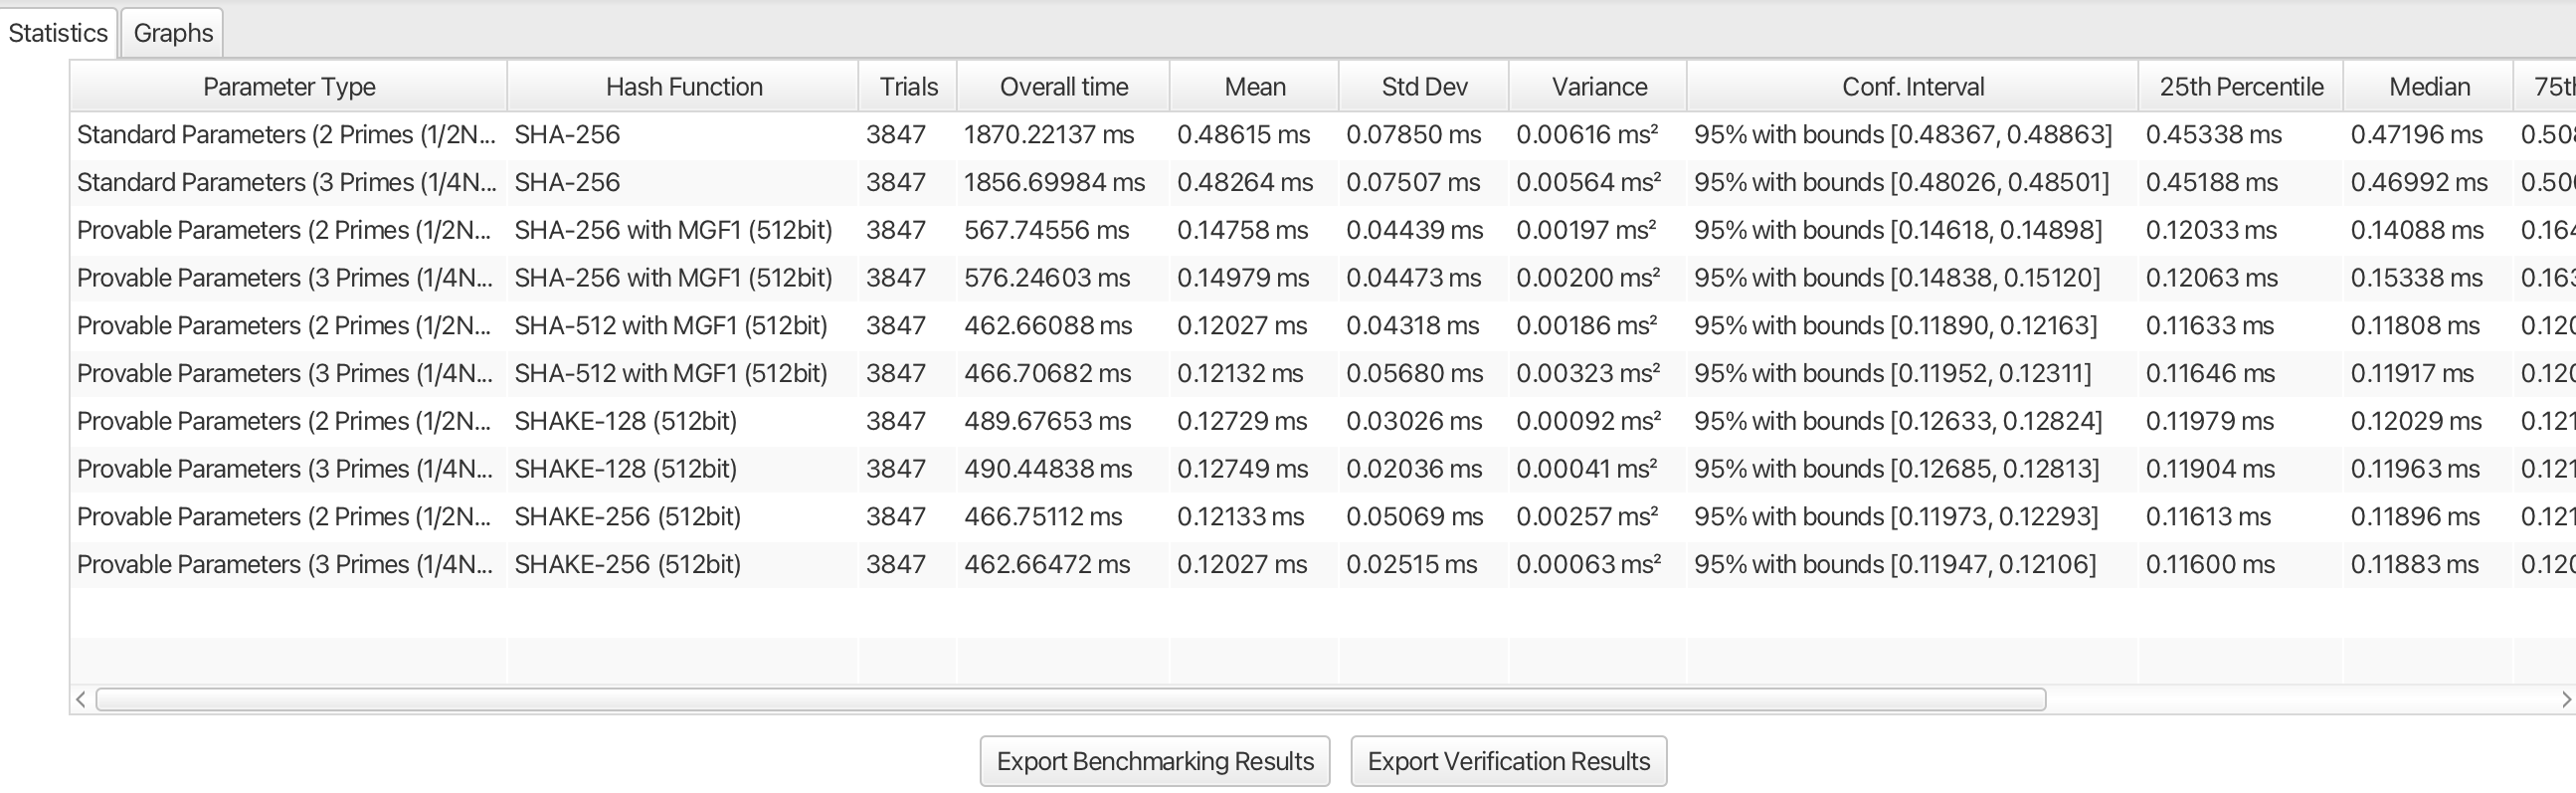
\includegraphics[width=\textwidth]{main_pictures/iso/iso_verify_1024bit_table1_1.png}} 
        \fbox{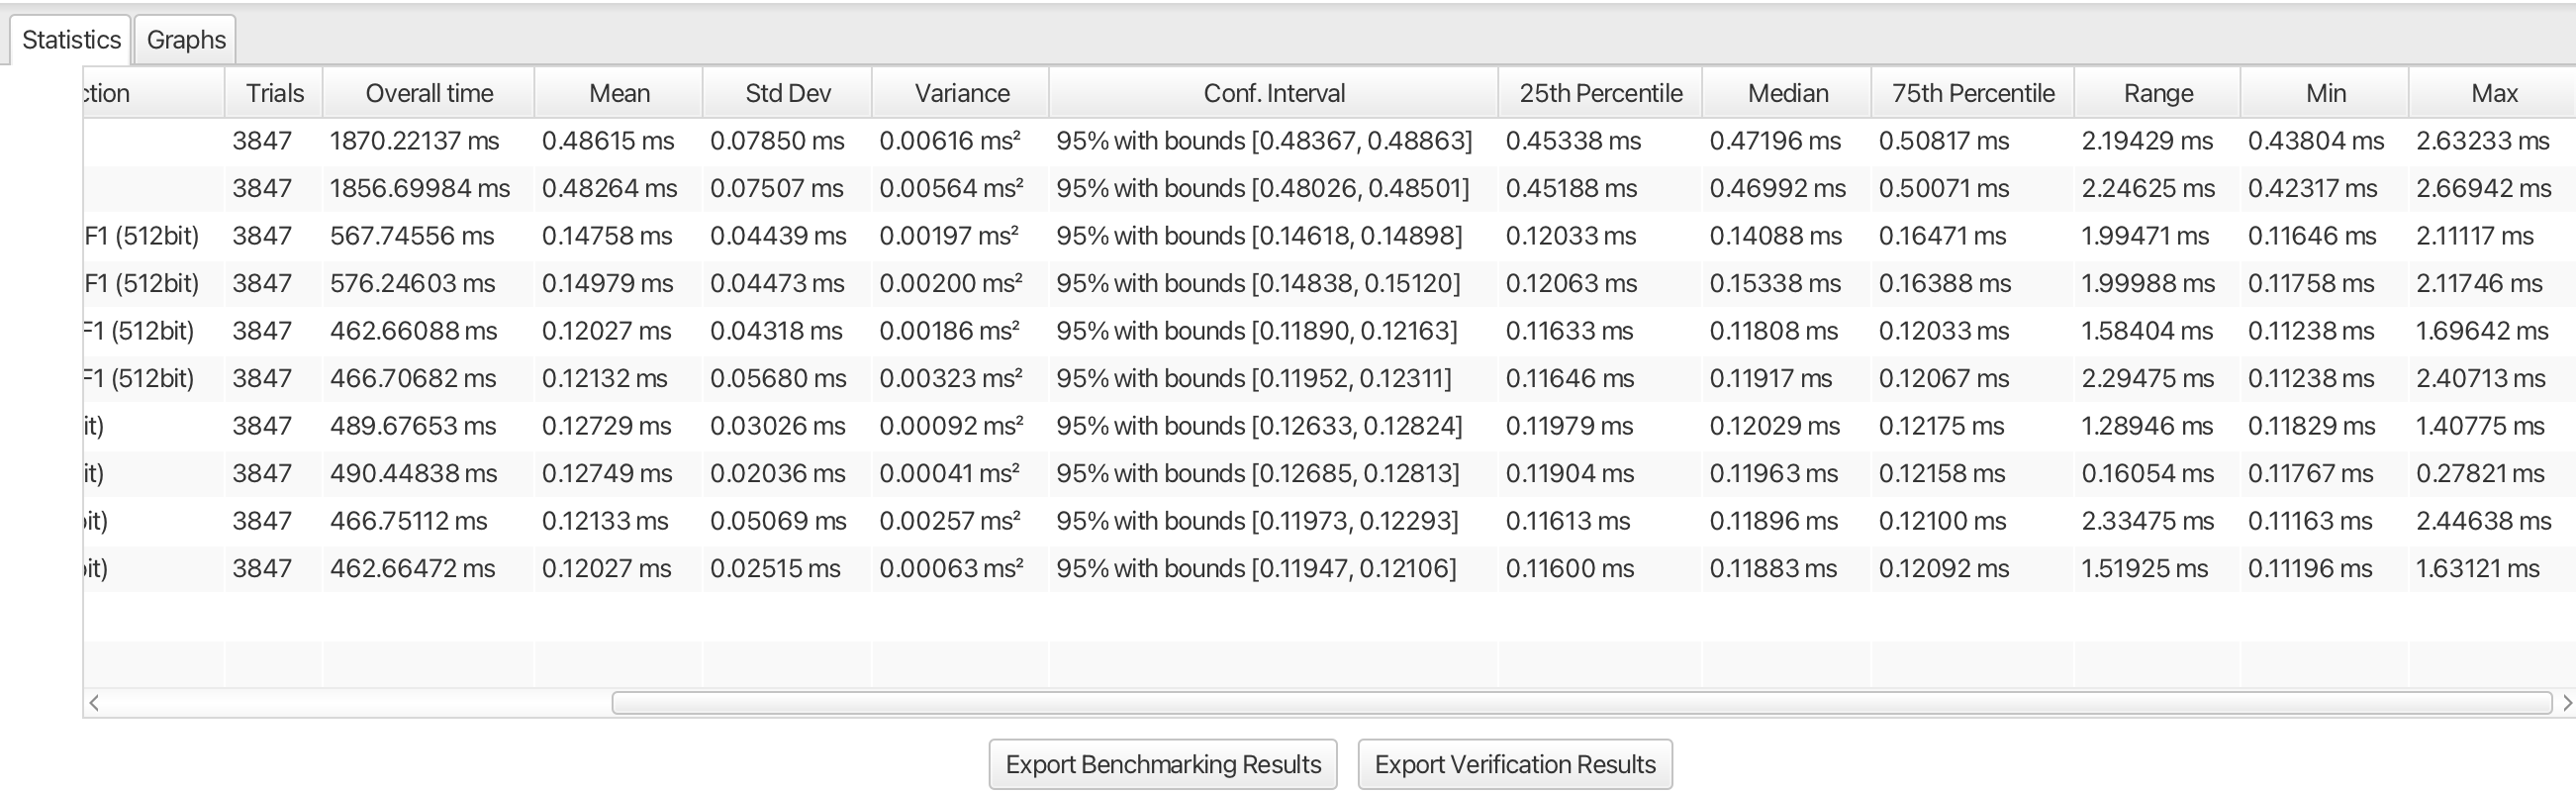
\includegraphics[width=\textwidth]{main_pictures/iso/iso_verify_1024bit_table2_1.png}}
    \end{minipage}
       \label{iso_verify_1024bit_table}
  \end{figure}
  
\begin{figure}[H]
    \centering % Center the images
     \caption{Instantiation of ISO/IEC 9796-2:2010 Signature Scheme 1 with standard vs provably secure parameters (2048-bit Key Size) for signature verification}
    % First image in a minipage
    \begin{minipage}{\textwidth}
        \centering
        \fbox{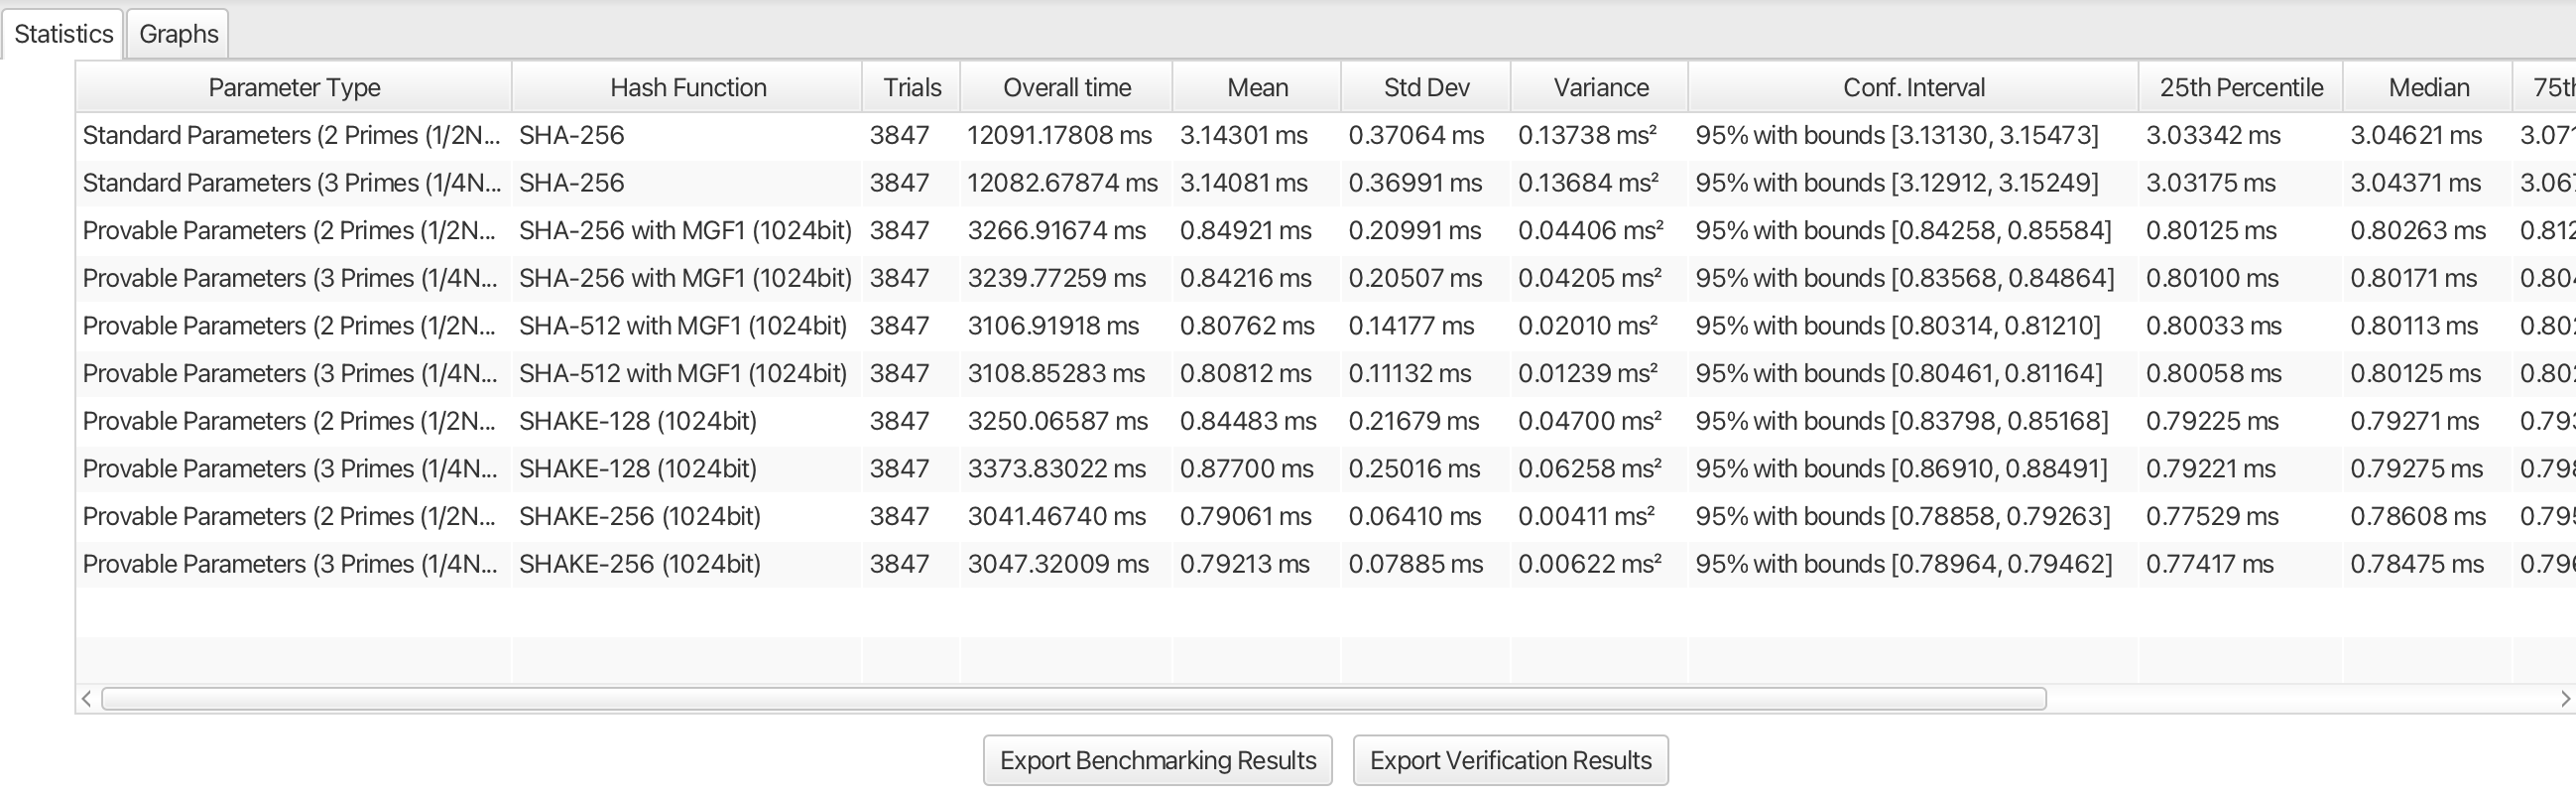
\includegraphics[width=\textwidth]{main_pictures/iso/iso_verify_2048bit_table1_1.png}} 
        \fbox{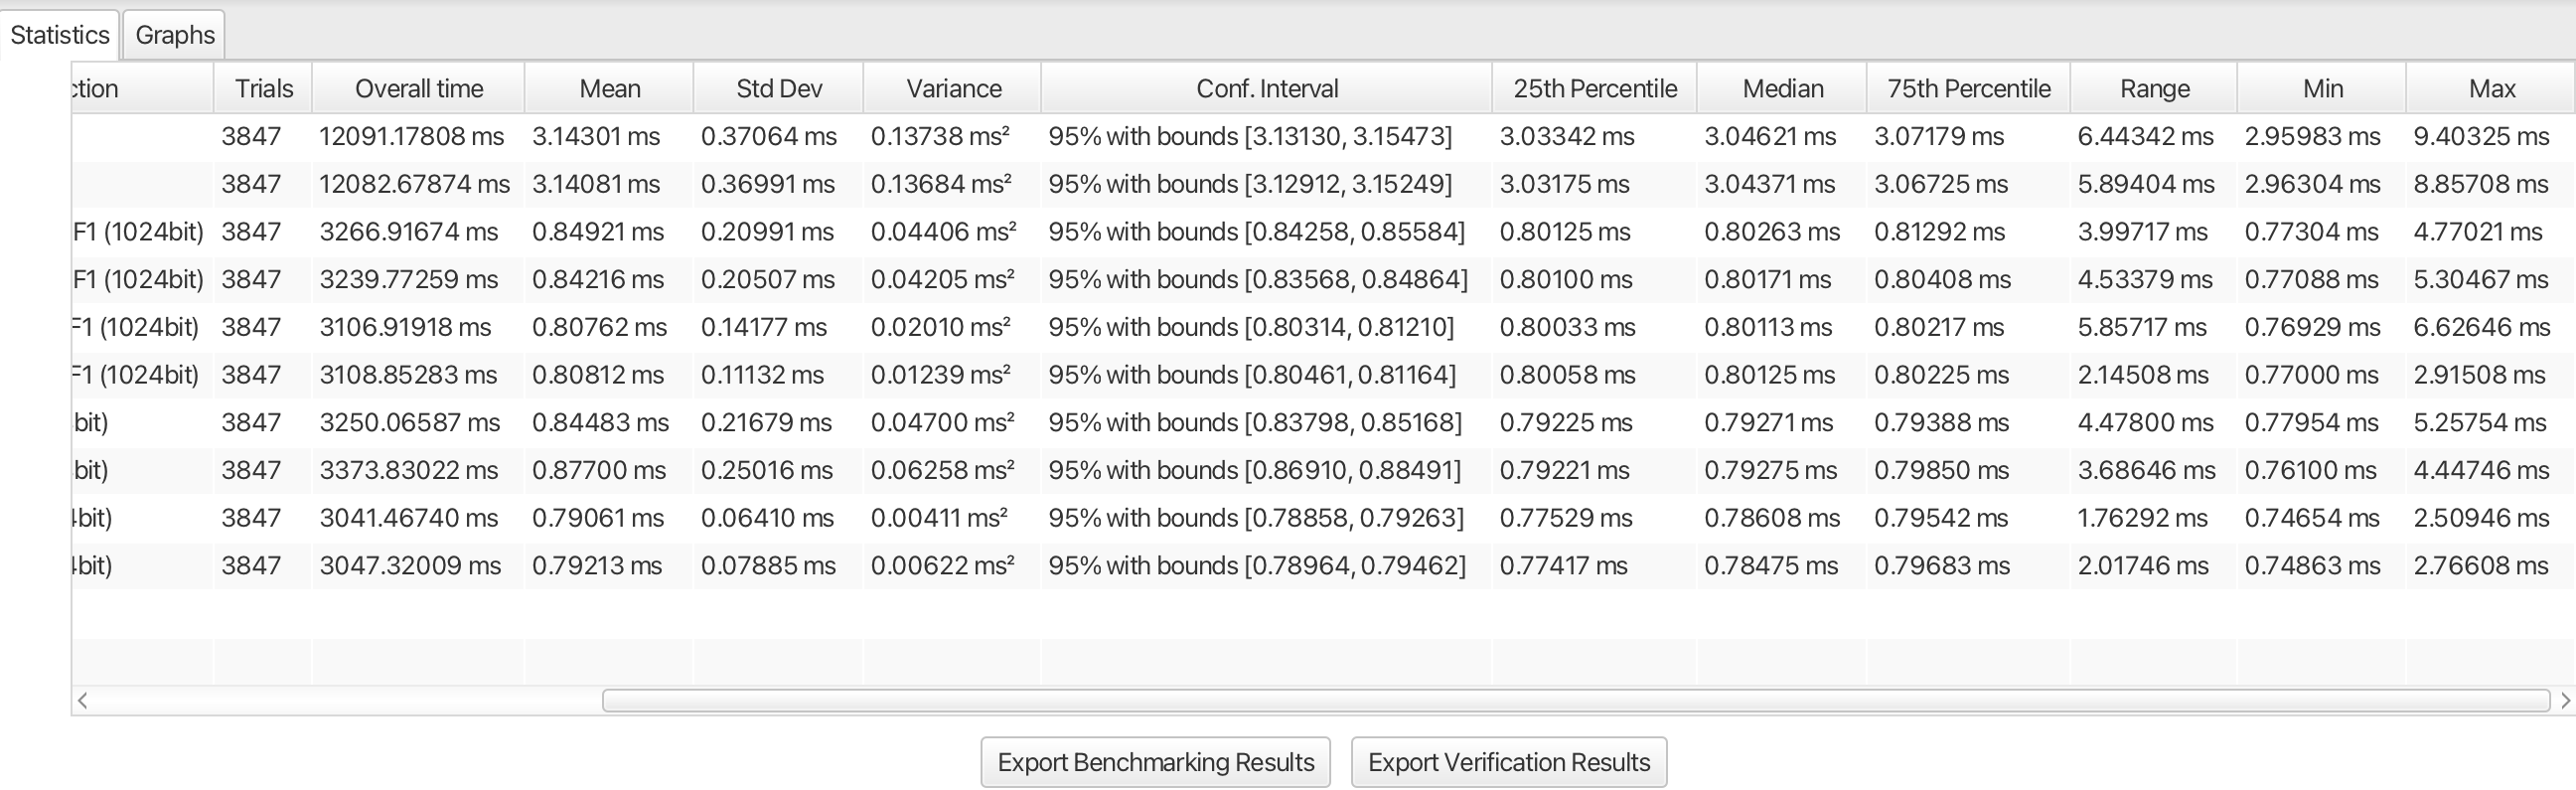
\includegraphics[width=\textwidth]{main_pictures/iso/iso_verify_2048bit_table2_1.png}}
    \end{minipage}
           \label{iso_verify_2048bit_table}
  \end{figure}
  
\begin{figure}[H]
    \centering % Center the images
     \caption{Instantiation of ISO/IEC 9796-2:2010 Signature Scheme 1 with standard vs provably secure parameters (3072-bit Key Size) for signature verification}
    % First image in a minipage
    \begin{minipage}{\textwidth}
        \centering
        \fbox{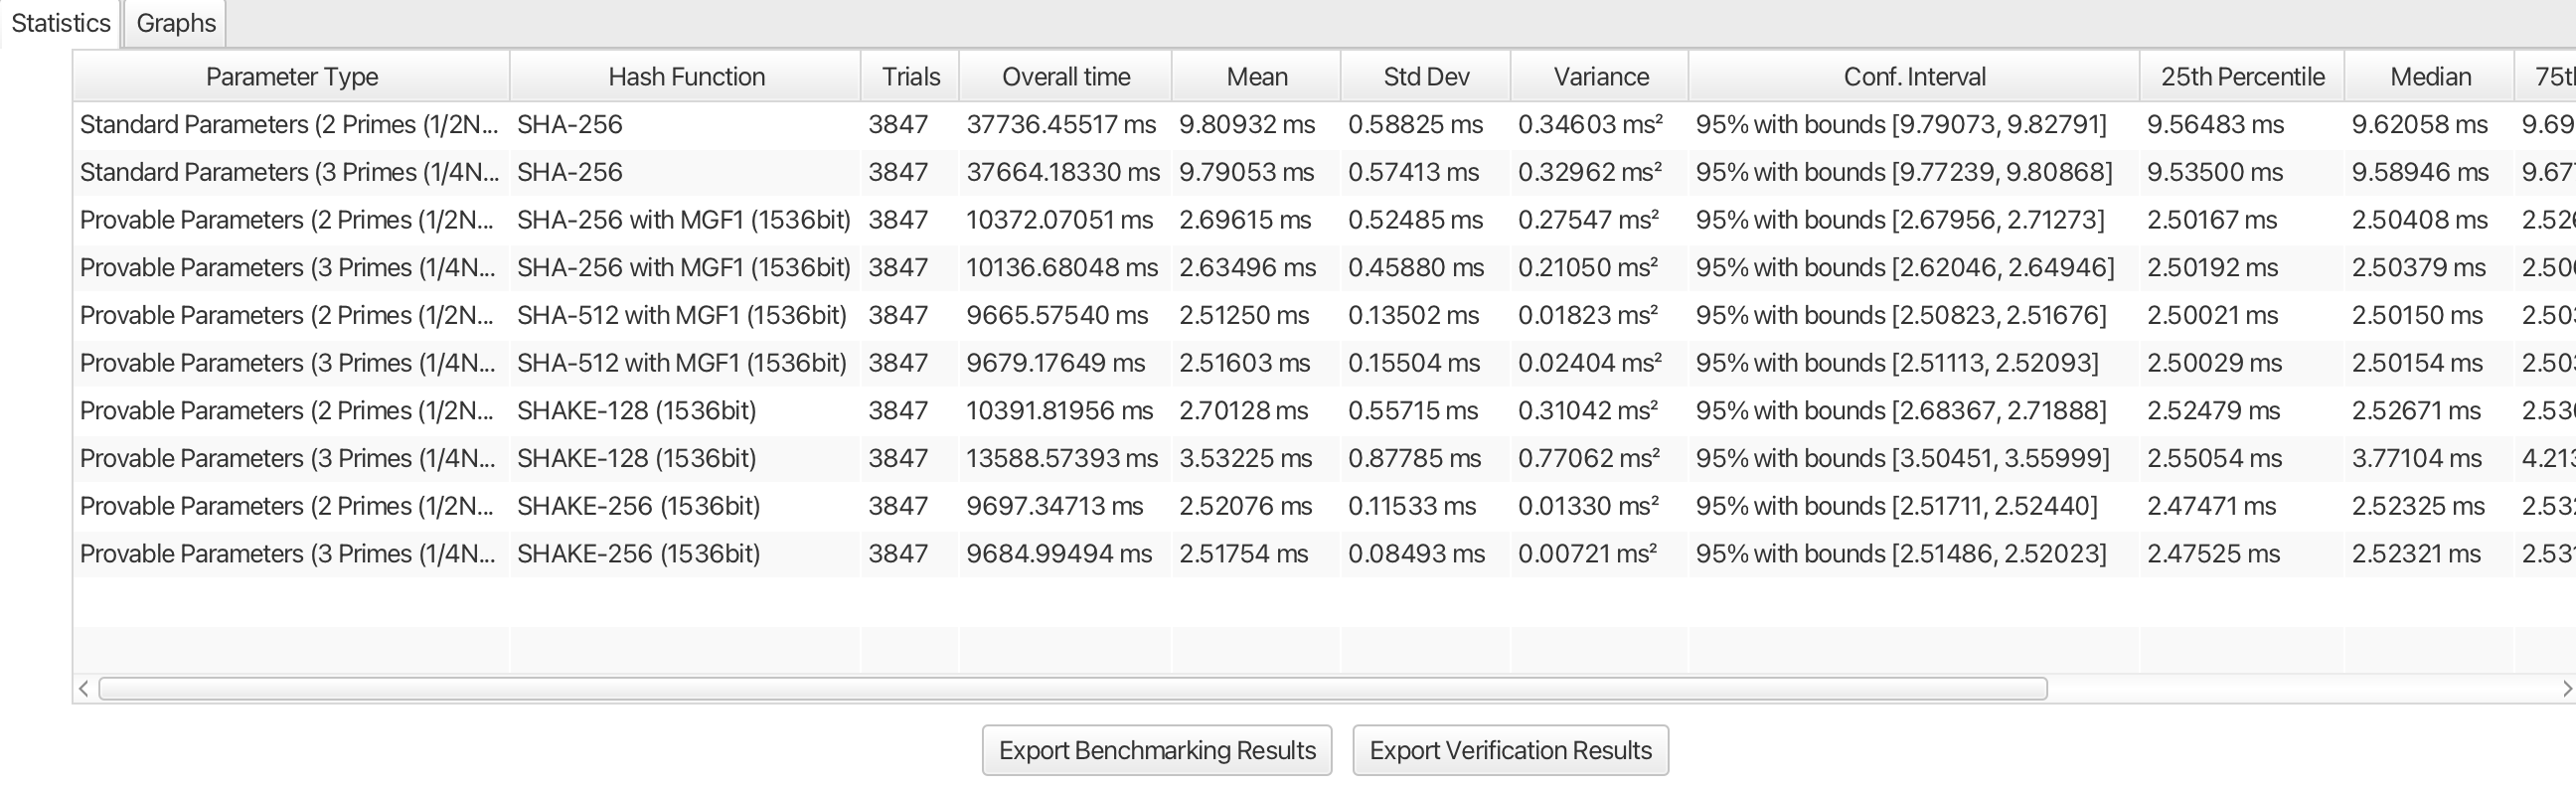
\includegraphics[width=\textwidth]{main_pictures/iso/iso_verify_3072bit_table1_1.png}} 
        \fbox{\includegraphics[width=\textwidth]{main_pictures/iso/iso_verify_3072bit_table2_1.png}}
    \end{minipage}
          \label{iso_verify_3072bit_table}
\end{figure}

\begin{figure}[H]
    \centering % Center the images
     \caption{Instantiation of ISO/IEC 9796-2:2010 Signature Scheme 1 with standard vs provably secure parameters (4096-bit Key Size) for signature verification}
    % First image in a minipage
    \begin{minipage}{\textwidth}
        \centering
        \fbox{\includegraphics[width=\textwidth]{main_pictures/iso/iso_verify_4096bit_table1_1.png}} 
        \fbox{\includegraphics[width=\textwidth]{main_pictures/iso/iso_verify_4096bit_table2_1.png}}
    \end{minipage}
         \label{iso_verify_4096bit_table}
\end{figure}

\begin{figure}[H]
    \centering % Center the images
     \caption{Instantiation of ISO/IEC 9796-2:2010 Signature Scheme 1 with standard vs provably secure parameters (5120-bit Key Size) for signature verification}
    % First image in a minipage
    \begin{minipage}{\textwidth}
        \centering
        \fbox{\includegraphics[width=\textwidth]{main_pictures/iso/iso_verify_5120bit_table1_1.png}} 
        \fbox{\includegraphics[width=\textwidth]{main_pictures/iso/iso_verify_5120bit_table2_1.png}}
    \end{minipage}
       \label{iso_verify_5120bit_table}
\end{figure}

\begin{figure}[H]
    \centering % Center the images
     \caption{Instantiation of ISO/IEC 9796-2:2010 Signature Scheme 1 with standard vs provably secure parameters (6144-bit Key Size) for signature verification}
    % First image in a minipage
    \begin{minipage}{\textwidth}
        \centering
        \fbox{\includegraphics[width=\textwidth]{main_pictures/iso/iso_verify_6144bit_table1_1.png}} 
        \fbox{\includegraphics[width=\textwidth]{main_pictures/iso/iso_verify_6144bit_table2_1.png}}
    \end{minipage}
         \label{iso_verify_6144bit_table}
\end{figure}
\end{comment}

\begin{landscape}
\pagestyle{empty}%

\section{Signature Verification Results (ISO/IEC 9796-2:2010 Signature Scheme 1)}

\begin{longtable}{|p{2.3cm}|p{1.8cm}|p{1.0cm}|p{1.7cm}|p{1.4cm}|p{1.5cm}|p{1.8cm}|p{1.5cm}|p{1.43cm}|p{1.5cm}|p{1.3cm}|p{1.4cm}|p{1.3cm}|p{1.3cm}|}

\caption{\textbf{Instantiation of ISO/IEC 9796-2:2010 Signature Scheme 1 with Standard vs Provably Secure Parameters (1024-bit Key Size) for Signature Verification}}
     \label{iso_verify_1024bit_table} \\
\hline
\textbf{Parameter Type} & \textbf{Hash Function} & \textbf{Trials} & \textbf{Overall Time} & \textbf{Mean} & \textbf{Std Dev} & \textbf{Variance} & \textbf{Conf. Interval} & \textbf{25th Percentile} & \textbf{Median} & \textbf{75th Percentile} & \textbf{Range} & \textbf{Min} & \textbf{Max} \\
\hline
\endfirsthead

\multicolumn{14}{c}%
{{\bfseries \tablename\ \thetable{} -- Signature Verification Results for ISO/IEC 9796-2:2010 Signature Scheme 1 with 1024-bit Key Size (continued from previous page)}} \\
\hline
\textbf{Parameter Type} & \textbf{Hash Function} & \textbf{Trials} & \textbf{Overall Time} & \textbf{Mean} & \textbf{Std Dev} & \textbf{Variance} & \textbf{Conf. Interval} & \textbf{25th Percentile} & \textbf{Median} & \textbf{75th Percentile} & \textbf{Range} & \textbf{Min} & \textbf{Max} \\
\hline
\endhead

\hline \multicolumn{14}{|r|}{{Continued on next page}} \\ \hline
\endfoot

\hline
\endlastfoot
Standard Parameters (2 Primes) & SHA-256 & 3847 & 1870.
22137 ms & 0.48615 ms & 0.07850 ms & 0.00616 ms\textsuperscript{2} & 95\% with bounds 0.48367 ms - 0.48863 ms & 0.45338 ms & 0.47196 ms & 0.50817 ms & 2.19429 ms & 0.43804 ms & 2.63233 ms \\
\hline
Standard Parameters (3 Primes) & SHA-256 & 3847 & 1856.
69984 ms & 0.48264 ms & 0.07507 ms & 0.00564 ms\textsuperscript{2} & 95\% with bounds 0.48026 ms - 0.48501 ms & 0.45188 ms & 0.46992 ms & 0.50071 ms & 2.24625 ms & 0.42317 ms & 2.66942 ms \\
\hline
Provable Parameters (2 Primes) & SHA-256 with MGF1 (512bit) & 3847 & 567.
74556 ms & 0.14758 ms & 0.04439 ms & 0.00197 ms\textsuperscript{2} & 95\% with bounds 0.14618 ms - 0.14898 ms & 0.12033 ms & 0.14088 ms & 0.16471 ms & 1.99471 ms & 0.11646 ms & 2.11117 ms \\
\hline
Provable Parameters (3 Primes) & SHA-256 with MGF1 (512bit) & 3847 & 576.
24603 ms & 0.14979 ms & 0.04473 ms & 0.00200 ms\textsuperscript{2} & 95\% with bounds 0.14838 ms - 0.15120 ms & 0.12063 ms & 0.15338 ms & 0.16388 ms & 1.99988 ms & 0.11758 ms & 2.11746 ms \\
\hline
Provable Parameters (2 Primes) & SHA-512 with MGF1 (512bit) & 3847 & 462.
66088 ms & 0.12027 ms & 0.04318 ms & 0.00186 ms\textsuperscript{2} & 95\% with bounds 0.11890 ms - 0.12163 ms & 0.11633 ms & 0.11808 ms & 0.12033 ms & 1.58404 ms & 0.11238 ms & 1.69642 ms \\
\hline
Provable Parameters (3 Primes) & SHA-512 with MGF1 (512bit) & 3847 & 466.
70682 ms & 0.12132 ms & 0.05680 ms & 0.00323 ms\textsuperscript{2} & 95\% with bounds 0.11952 ms - 0.12311 ms & 0.11646 ms & 0.11917 ms & 0.12067 ms & 2.29475 ms & 0.11238 ms & 2.40713 ms \\
\hline
Provable Parameters (2 Primes) & SHAKE-128 (512bit) & 3847 & 489.
67653 ms & 0.12729 ms & 0.03026 ms & 0.00092 ms\textsuperscript{2} & 95\% with bounds 0.12633 ms - 0.12824 ms & 0.11979 ms & 0.12029 ms & 0.12175 ms & 1.28946 ms & 0.11829 ms & 1.40775 ms \\
\hline
Provable Parameters (3 Primes) & SHAKE-128 (512bit) & 3847 & 490.
44838 ms & 0.12749 ms & 0.02036 ms & 0.00041 ms\textsuperscript{2} & 95\% with bounds 0.12685 ms - 0.12813 ms & 0.11904 ms & 0.11963 ms & 0.12158 ms & 0.16054 ms & 0.11767 ms & 0.27821 ms \\
\hline
Provable Parameters (2 Primes) & SHAKE-256 (512bit) & 3847 & 466.
75112 ms & 0.12133 ms & 0.05069 ms & 0.00257 ms\textsuperscript{2} & 95\% with bounds 0.11973 ms - 0.12293 ms & 0.11613 ms & 0.11896 ms & 0.12100 ms & 2.33475 ms & 0.11163 ms & 2.44638 ms \\
\hline
Provable Parameters (3 Primes) & SHAKE-256 (512bit) & 3847 & 462.
66472 ms & 0.12027 ms & 0.02515 ms & 0.00063 ms\textsuperscript{2} & 95\% with bounds 0.11947 ms - 0.12106 ms & 0.11600 ms & 0.11883 ms & 0.12092 ms & 1.51925 ms & 0.11196 ms & 1.63121 ms \\
\hline
\end{longtable}

\begin{longtable}{|p{2.3cm}|p{1.8cm}|p{1.0cm}|p{1.7cm}|p{1.4cm}|p{1.5cm}|p{1.8cm}|p{1.5cm}|p{1.43cm}|p{1.5cm}|p{1.3cm}|p{1.4cm}|p{1.3cm}|p{1.3cm}|}

\caption{\textbf{Instantiation of ISO/IEC 9796-2:2010 Signature Scheme 1 with Standard vs Provably Secure Parameters (2048-bit Key Size) for Signature Verification}}
     \label{iso_verify_2048bit_table} \\
\hline
\textbf{Parameter Type} & \textbf{Hash Function} & \textbf{Trials} & \textbf{Overall Time} & \textbf{Mean} & \textbf{Std Dev} & \textbf{Variance} & \textbf{Conf. Interval} & \textbf{25th Percentile} & \textbf{Median} & \textbf{75th Percentile} & \textbf{Range} & \textbf{Min} & \textbf{Max} \\
\hline
\endfirsthead

\multicolumn{14}{c}%
{{\bfseries \tablename\ \thetable{} -- Signature Verification Results for ISO/IEC 9796-2:2010 Signature Scheme 1 with 2048-bit Key Size (continued from previous page)}} \\
\hline
\textbf{Parameter Type} & \textbf{Hash Function} & \textbf{Trials} & \textbf{Overall Time} & \textbf{Mean} & \textbf{Std Dev} & \textbf{Variance} & \textbf{Conf. Interval} & \textbf{25th Percentile} & \textbf{Median} & \textbf{75th Percentile} & \textbf{Range} & \textbf{Min} & \textbf{Max} \\
\hline
\endhead

\hline \multicolumn{14}{|r|}{{Continued on next page}} \\ \hline
\endfoot

\hline
\endlastfoot
Standard Parameters (2 Primes) & SHA-256 & 3847 & 12091.
17808 ms & 3.14301 ms & 0.37064 ms & 0.13738 ms\textsuperscript{2} & 95\% with bounds 3.13130 ms - 3.15473 ms & 3.03342 ms & 3.04621 ms & 3.07179 ms & 6.44342 ms & 2.95983 ms & 9.40325 ms \\
\hline
Standard Parameters (3 Primes) & SHA-256 & 3847 & 12082.
67874 ms & 3.14081 ms & 0.36991 ms & 0.13684 ms\textsuperscript{2} & 95\% with bounds 3.12912 ms - 3.15249 ms & 3.03175 ms & 3.04371 ms & 3.06725 ms & 5.89404 ms & 2.96304 ms & 8.85708 ms \\
\hline
Provable Parameters (2 Primes) & SHA-256 with MGF1 (1024bit) & 3847 & 3266.
91674 ms & 0.84921 ms & 0.20991 ms & 0.04406 ms\textsuperscript{2} & 95\% with bounds 0.84258 ms - 0.85584 ms & 0.80125 ms & 0.80263 ms & 0.81292 ms & 3.99717 ms & 0.77304 ms & 4.77021 ms \\
\hline
Provable Parameters (3 Primes) & SHA-256 with MGF1 (1024bit) & 3847 & 3239.
77259 ms & 0.84216 ms & 0.20507 ms & 0.04205 ms\textsuperscript{2} & 95\% with bounds 0.83568 ms - 0.84864 ms & 0.80100 ms & 0.80171 ms & 0.80408 ms & 4.53379 ms & 0.77088 ms & 5.30467 ms \\
\hline
Provable Parameters (2 Primes) & SHA-512 with MGF1 (1024bit) & 3847 & 3106.
91918 ms & 0.80762 ms & 0.14177 ms & 0.02010 ms\textsuperscript{2} & 95\% with bounds 0.80314 ms - 0.81210 ms & 0.80033 ms & 0.80113 ms & 0.80217 ms & 5.85717 ms & 0.76929 ms & 6.62646 ms \\
\hline
Provable Parameters (3 Primes) & SHA-512 with MGF1 (1024bit) & 3847 & 3108.
85283 ms & 0.80812 ms & 0.11132 ms & 0.01239 ms\textsuperscript{2} & 95\% with bounds 0.80461 ms - 0.81164 ms & 0.80058 ms & 0.80125 ms & 0.80225 ms & 2.14508 ms & 0.77000 ms & 2.91508 ms \\
\hline
Provable Parameters (2 Primes) & SHAKE-128 (1024bit) & 3847 & 3250.
06587 ms & 0.84483 ms & 0.21679 ms & 0.04700 ms\textsuperscript{2} & 95\% with bounds 0.83798 ms - 0.85168 ms & 0.79225 ms & 0.79271 ms & 0.79388 ms & 4.47800 ms & 0.77954 ms & 5.25754 ms \\
\hline
Provable Parameters (3 Primes) & SHAKE-128 (1024bit) & 3847 & 3373.
83022 ms & 0.87700 ms & 0.25016 ms & 0.06258 ms\textsuperscript{2} & 95\% with bounds 0.86910 ms - 0.88491 ms & 0.79221 ms & 0.79275 ms & 0.79850 ms & 3.68646 ms & 0.76100 ms & 4.44746 ms \\
\hline
Provable Parameters (2 Primes) & SHAKE-256 (1024bit) & 3847 & 3041.
46740 ms & 0.79061 ms & 0.06410 ms & 0.00411 ms\textsuperscript{2} & 95\% with bounds 0.78858 ms - 0.79263 ms & 0.77529 ms & 0.78608 ms & 0.79542 ms & 1.76292 ms & 0.74654 ms & 2.50946 ms \\
\hline
Provable Parameters (3 Primes) & SHAKE-256 (1024bit) & 3847 & 3047.3
2009 ms & 0.79213 ms & 0.07885 ms & 0.00622 ms\textsuperscript{2} & 95\% with bounds 0.78964 ms - 0.79462 ms & 0.77417 ms & 0.78475 ms & 0.79683 ms & 2.01746 ms & 0.74863 ms & 2.76608 ms \\
\hline




\end{longtable}


\begin{longtable}{|p{2.3cm}|p{1.8cm}|p{1.0cm}|p{1.7cm}|p{1.4cm}|p{1.5cm}|p{1.8cm}|p{1.5cm}|p{1.43cm}|p{1.5cm}|p{1.3cm}|p{1.4cm}|p{1.3cm}|p{1.3cm}|}

\caption{\textbf{Instantiation of ISO/IEC 9796-2:2010 Signature Scheme 1 with Standard vs Provably Secure Parameters (3072-bit Key Size) for Signature Verification}}
     \label{iso_verify_3072bit_table} \\
\hline
\textbf{Parameter Type} & \textbf{Hash Function} & \textbf{Trials} & \textbf{Overall Time} & \textbf{Mean} & \textbf{Std Dev} & \textbf{Variance} & \textbf{Conf. Interval} & \textbf{25th Percentile} & \textbf{Median} & \textbf{75th Percentile} & \textbf{Range} & \textbf{Min} & \textbf{Max} \\
\hline
\endfirsthead

\multicolumn{14}{c}%
{{\bfseries \tablename\ \thetable{} -- Signature Verification Results for ISO/IEC 9796-2:2010 Signature Scheme 1 with 3072-bit Key Size (continued from previous page)}} \\
\hline
\textbf{Parameter Type} & \textbf{Hash Function} & \textbf{Trials} & \textbf{Overall Time} & \textbf{Mean} & \textbf{Std Dev} & \textbf{Variance} & \textbf{Conf. Interval} & \textbf{25th Percentile} & \textbf{Median} & \textbf{75th Percentile} & \textbf{Range} & \textbf{Min} & \textbf{Max} \\
\hline
\endhead

\hline \multicolumn{14}{|r|}{{Continued on next page}} \\ \hline
\endfoot

\hline
\endlastfoot
Standard Parameters (2 Primes) & SHA-256 & 3847 & 37736.
45517 ms & 9.80932 ms & 0.58825 ms & 0.34603 ms\textsuperscript{2} & 95\% with bounds 9.79073 ms - 9.82791 ms & 9.56483 ms & 9.62058 ms & 9.69996 ms & 16.85458 ms & 9.35346 ms & 26.20804 ms \\
\hline
Standard Parameters (3 Primes) & SHA-256 & 3847 & 37664.
18330 ms & 9.79053 ms & 0.57413 ms & 0.32962 ms\textsuperscript{2} & 95\% with bounds 9.77239 ms - 9.80868 ms & 9.53500 ms & 9.58946 ms & 9.67729 ms & 14.68250 ms & 9.34133 ms & 24.02383 ms \\
\hline
Provable Parameters (2 Primes) & SHA-256 with MGF1 (1536bit) & 3847 & 10372.
07051 ms & 2.69615 ms & 0.52485 ms & 0.27547 ms\textsuperscript{2} & 95\% with bounds 2.67956 ms - 2.71273 ms & 2.50167 ms & 2.50408 ms & 2.52675 ms & 5.66167 ms & 2.41333 ms & 8.07500 ms \\
\hline
Provable Parameters (3 Primes) & SHA-256 with MGF1 (1536bit) & 3847 & 10136.
68048 ms & 2.63496 ms & 0.45880 ms & 0.21050 ms\textsuperscript{2} & 95\% with bounds 2.62046 ms - 2.64946 ms & 2.50192 ms & 2.50379 ms & 2.50683 ms & 4.13346 ms & 2.42083 ms & 6.55429 ms \\
\hline
Provable Parameters (2 Primes) & SHA-512 with MGF1 (1536bit) & 3847 & 9665.
57540 ms & 2.51250 ms & 0.13502 ms & 0.01823 ms\textsuperscript{2} & 95\% with bounds 2.50823 ms - 2.51676 ms & 2.50021 ms & 2.50150 ms & 2.50313 ms & 2.13779 ms & 2.41192 ms & 4.54971 ms \\
\hline
Provable Parameters (3 Primes) & SHA-512 with MGF1 (1536bit) & 3847 & 9679.
17649 ms & 2.51603 ms & 0.15504 ms & 0.02404 ms\textsuperscript{2} & 95\% with bounds 2.51113 ms - 2.52093 ms & 2.50029 ms & 2.50154 ms & 2.50313 ms & 3.15913 ms & 2.40388 ms & 5.56300 ms \\
\hline
Provable Parameters (2 Primes) & SHAKE-128 (1536bit) & 3847 & 10391.
81956 ms & 2.70128 ms & 0.55715 ms & 0.31042 ms\textsuperscript{2} & 95\% with bounds 2.68367 ms - 2.71888 ms & 2.52479 ms & 2.52671 ms & 2.53029 ms & 4.85117 ms & 2.46354 ms & 7.31471 ms \\
\hline
Provable Parameters (3 Primes) & SHAKE-128 (1536bit) & 3847 & 13588.
57393 ms & 3.53225 ms & 0.87785 ms & 0.77062 ms\textsuperscript{2} & 95\% with bounds 3.50451 ms - 3.55999 ms & 2.55054 ms & 3.77104 ms & 4.21304 ms & 4.34313 ms & 2.45088 ms & 6.79400 ms \\
\hline
Provable Parameters (2 Primes) & SHAKE-256 (1536bit) & 3847 & 9697.
34713 ms & 2.52076 ms & 0.11533 ms & 0.01330 ms\textsuperscript{2} & 95\% with bounds 2.51711 ms - 2.52440 ms & 2.47471 ms & 2.52325 ms & 2.53258 ms & 2.70246 ms & 2.41908 ms & 5.12154 ms \\
\hline
Provable Parameters (3 Primes) & SHAKE-256 (1536bit) & 3847 & 9684.
99494 ms & 2.51754 ms & 0.08493 ms & 0.00721 ms\textsuperscript{2} & 95\% with bounds 2.51486 ms - 2.52023 ms & 2.47525 ms & 2.52321 ms & 2.53113 ms & 2.50767 ms & 2.37942 ms & 4.88708 ms \\
\hline
\end{longtable}



\begin{longtable}{|p{2.3cm}|p{1.8cm}|p{1.0cm}|p{1.7cm}|p{1.4cm}|p{1.5cm}|p{1.8cm}|p{1.5cm}|p{1.43cm}|p{1.5cm}|p{1.3cm}|p{1.4cm}|p{1.3cm}|p{1.3cm}|}

\caption{\textbf{Instantiation of ISO/IEC 9796-2:2010 Signature Scheme 1 with Standard vs Provably Secure Parameters (4096-bit Key Size) for Signature Verification}}
     \label{iso_verify_4096bit_table} \\
\hline
\textbf{Parameter Type} & \textbf{Hash Function} & \textbf{Trials} & \textbf{Overall Time} & \textbf{Mean} & \textbf{Std Dev} & \textbf{Variance} & \textbf{Conf. Interval} & \textbf{25th Percentile} & \textbf{Median} & \textbf{75th Percentile} & \textbf{Range} & \textbf{Min} & \textbf{Max} \\
\hline
\endfirsthead

\multicolumn{14}{c}%
{{\bfseries \tablename\ \thetable{} -- Signature Verification Results for ISO/IEC 9796-2:2010 Signature Scheme 1 with 4096-bit Key Size (continued from previous page)}} \\
\hline
\textbf{Parameter Type} & \textbf{Hash Function} & \textbf{Trials} & \textbf{Overall Time} & \textbf{Mean} & \textbf{Std Dev} & \textbf{Variance} & \textbf{Conf. Interval} & \textbf{25th Percentile} & \textbf{Median} & \textbf{75th Percentile} & \textbf{Range} & \textbf{Min} & \textbf{Max} \\
\hline
\endhead

\hline \multicolumn{14}{|r|}{{Continued on next page}} \\ \hline
\endfoot

\hline
\endlastfoot
Standard Parameters (2 Primes) & SHA-256 & 3847 & 86729.
04912 ms & 22.54459 ms & 0.99766 ms & 0.99533 ms\textsuperscript{2} & 95\% with bounds 22.51307 ms - 22.57612 ms & 22.10546 ms & 22.16746 ms & 22.29513 ms & 20.34475 ms & 21.67038 ms & 42.01513 ms \\
\hline
Standard Parameters (3 Primes) & SHA-256 & 3847 & 86478.
65081 ms & 22.47950 ms & 0.94668 ms & 0.89620 ms\textsuperscript{2} & 95\% with bounds 22.44959 ms - 22.50942 ms & 22.04025 ms & 22.09213 ms & 22.23721 ms & 9.65617 ms & 21.60875 ms & 31.26492 ms \\
\hline
Provable Parameters (2 Primes) & SHA-256 with MGF1 (2048bit) & 3847 & 23568.
56889 ms & 6.12648 ms & 0.89830 ms & 0.80694 ms\textsuperscript{2} & 95\% with bounds 6.09809 ms - 6.15487 ms & 5.79229 ms & 5.79975 ms & 5.81546 ms & 6.60117 ms & 5.65004 ms & 12.25121 ms \\
\hline
Provable Parameters (3 Primes) & SHA-256 with MGF1 (2048bit) & 3847 & 23506.
93994 ms & 6.11046 ms & 0.89671 ms & 0.80409 ms\textsuperscript{2} & 95\% with bounds 6.08212 ms - 6.13880 ms & 5.79088 ms & 5.79563 ms & 5.80767 ms & 7.41688 ms & 5.62392 ms & 13.04079 ms \\
\hline
Provable Parameters (2 Primes) & SHA-512 with MGF1 (2048bit) & 3847 & 22940.
43005 ms & 5.96320 ms & 0.51409 ms & 0.26429 ms\textsuperscript{2} & 95\% with bounds 5.94695 ms - 5.97945 ms & 5.79396 ms & 5.80517 ms & 5.85058 ms & 6.71479 ms & 5.59104 ms & 12.30583 ms \\
\hline
Provable Parameters (3 Primes) & SHA-512 with MGF1 (2048bit) & 3847 & 22638.
16787 ms & 5.88463 ms & 0.36970 ms & 0.13668 ms\textsuperscript{2} & 95\% with bounds 5.87295 ms - 5.89631 ms & 5.79200 ms & 5.79613 ms & 5.80625 ms & 5.06275 ms & 5.59238 ms & 10.65513 ms \\
\hline
Provable Parameters (2 Primes) & SHAKE-128 (2048bit) & 3847 & 23508.
71439 ms & 6.11092 ms & 1.06869 ms & 1.14210 ms\textsuperscript{2} & 95\% with bounds 6.07715 ms - 6.14469 ms & 5.79600 ms & 5.79946 ms & 5.80538 ms & 8.41121 ms & 5.65317 ms & 14.06438 ms \\
\hline
Provable Parameters (3 Primes) & SHAKE-128 (2048bit) & 3847 & 32738.
83044 ms & 8.51022 ms & 1.60698 ms & 2.58237 ms\textsuperscript{2} & 95\% with bounds 8.45944 ms - 8.56100 ms & 7.11367 ms & 9.35804 ms & 9.64050 ms & 8.62363 ms & 5.66679 ms & 14.29042 ms \\
\hline
Provable Parameters (2 Primes) & SHAKE-256 (2048bit) & 3847 & 22973.
66314 ms & 5.97184 ms & 0.36749 ms & 0.13505 ms\textsuperscript{2} & 95\% with bounds 5.96023 ms - 5.98345 ms & 5.79392 ms & 5.84183 ms & 6.05367 ms & 5.07046 ms & 5.55875 ms & 10.62921 ms \\
\hline
Provable Parameters (3 Primes) & SHAKE-256 (2048bit) & 3847 & 23078.
84076 ms & 5.99918 ms & 0.48428 ms & 0.23453 ms\textsuperscript{2} & 95\% with bounds 5.98388 ms - 6.01448 ms & 5.79921 ms & 5.81863 ms & 5.90775 ms & 4.87288 ms & 5.53375 ms & 10.40663 ms \\
\hline
\end{longtable}


\begin{longtable}{|p{2.3cm}|p{1.8cm}|p{1.0cm}|p{1.7cm}|p{1.4cm}|p{1.5cm}|p{1.8cm}|p{1.5cm}|p{1.43cm}|p{1.5cm}|p{1.3cm}|p{1.4cm}|p{1.3cm}|p{1.3cm}|}

\caption{\textbf{Instantiation of ISO/IEC 9796-2:2010 Signature Scheme 1 with Standard vs Provably Secure Parameters (5120-bit Key Size) for Signature Verification}}
     \label{iso_verify_5120bit_table} \\
\hline
\textbf{Parameter Type} & \textbf{Hash Function} & \textbf{Trials} & \textbf{Overall Time} & \textbf{Mean} & \textbf{Std Dev} & \textbf{Variance} & \textbf{Conf. Interval} & \textbf{25th Percentile} & \textbf{Median} & \textbf{75th Percentile} & \textbf{Range} & \textbf{Min} & \textbf{Max} \\
\hline
\endfirsthead

\multicolumn{14}{c}%
{{\bfseries \tablename\ \thetable{} -- Signature Verification Results for ISO/IEC 9796-2:2010 Signature Scheme 1 with 5120-bit Key Size (continued from previous page)}} \\
\hline
\textbf{Parameter Type} & \textbf{Hash Function} & \textbf{Trials} & \textbf{Overall Time} & \textbf{Mean} & \textbf{Std Dev} & \textbf{Variance} & \textbf{Conf. Interval} & \textbf{25th Percentile} & \textbf{Median} & \textbf{75th Percentile} & \textbf{Range} & \textbf{Min} & \textbf{Max} \\
\hline
\endhead

\hline \multicolumn{14}{|r|}{{Continued on next page}} \\ \hline
\endfoot

\hline
\endlastfoot
Standard Parameters (2 Primes) & SHA-256 & 3847 & 166964.
01566 ms & 43.40110 ms & 1.78770 ms & 3.19589 ms\textsuperscript{2} & 95\% with bounds 43.34460 ms - 43.45759 ms & 42.32921 ms & 42.54483 ms & 43.78004 ms & 18.73504 ms & 41.50908 ms & 60.24413 ms \\
\hline
Standard Parameters (3 Primes) & SHA-256 & 3847 & 166977.
10477 ms & 43.40450 ms & 1.80758 ms & 3.26736 ms\textsuperscript{2} & 95\% with bounds 43.34738 ms - 43.46162 ms & 42.32650 ms & 42.54958 ms & 43.72804 ms & 16.22946 ms & 41.33225 ms & 57.56171 ms \\
\hline
Provable Parameters (2 Primes) & SHA-256 with MGF1 (2560bit) & 3847 & 46238.
80486 ms & 12.01944 ms & 1.74923 ms & 3.05980 ms\textsuperscript{2} & 95\% with bounds 11.96417 ms - 12.07472 ms & 11.06104 ms & 11.21483 ms & 11.99758 ms & 26.92771 ms & 10.64492 ms & 37.57263 ms \\
\hline
Provable Parameters (3 Primes) & SHA-256 with MGF1 (2560bit) & 3847 & 44934.
87601 ms & 11.68050 ms & 1.37762 ms & 1.89784 ms\textsuperscript{2} & 95\% with bounds 11.63697 ms - 11.72403 ms & 11.04392 ms & 11.10175 ms & 11.66979 ms & 13.99221 ms & 10.73888 ms & 24.73108 ms \\
\hline
Provable Parameters (2 Primes) & SHA-512 with MGF1 (2560bit) & 3847 & 43896.
27344 ms & 11.41052 ms & 0.93217 ms & 0.86894 ms\textsuperscript{2} & 95\% with bounds 11.38106 ms - 11.43998 ms & 11.04304 ms & 11.05863 ms & 11.37525 ms & 10.62117 ms & 10.73017 ms & 21.35133 ms \\
\hline
Provable Parameters (3 Primes) & SHA-512 with MGF1 (2560bit) & 3847 & 43591.
86995 ms & 11.33139 ms & 0.90508 ms & 0.81918 ms\textsuperscript{2} & 95\% with bounds 11.30279 ms - 11.35999 ms & 11.03996 ms & 11.04817 ms & 11.14654 ms & 9.00083 ms & 10.71758 ms & 19.71842 ms \\
\hline
Provable Parameters (2 Primes) & SHAKE-128 (2560bit) & 3847 & 44534.
87892 ms & 11.57652 ms & 1.74601 ms & 3.04854 ms\textsuperscript{2} & 95\% with bounds 11.52135 ms - 11.63170 ms & 11.04567 ms & 11.05083 ms & 11.09825 ms & 16.66925 ms & 10.70621 ms & 27.37546 ms \\
\hline
Provable Parameters (3 Primes) & SHAKE-128 (2560bit) & 3847 & 59489.
24717 ms & 15.46380 ms & 2.65456 ms & 7.04669 ms\textsuperscript{2} & 95\% with bounds 15.37992 ms - 15.54769 ms & 13.03546 ms & 15.92725 ms & 17.68492 ms & 14.11558 ms & 10.72654 ms & 24.84213 ms \\
\hline
Provable Parameters (2 Primes) & SHAKE-256 (2560bit) & 3847 & 49624.
27619 ms & 12.89947 ms & 1.48181 ms & 2.19575 ms\textsuperscript{2} & 95\% with bounds 12.85265 ms - 12.94630 ms & 11.33158 ms & 12.88388 ms & 14.20288 ms & 7.40663 ms & 10.67579 ms & 18.08242 ms \\
\hline
Provable Parameters (3 Primes) & SHAKE-256 (2560bit) & 3847 & 47462.
74155 ms & 12.33760 ms & 1.53200 ms & 2.34703 ms\textsuperscript{2} & 95\% with bounds 12.28919 ms - 12.38601 ms & 11.14038 ms & 11.53213 ms & 13.56283 ms & 10.44763 ms & 10.67229 ms & 21.11992 ms \\
\hline


\end{longtable}


\begin{longtable}{|p{2.3cm}|p{1.8cm}|p{1.0cm}|p{1.7cm}|p{1.4cm}|p{1.5cm}|p{1.8cm}|p{1.5cm}|p{1.43cm}|p{1.5cm}|p{1.3cm}|p{1.4cm}|p{1.3cm}|p{1.37cm}|}

\caption{\textbf{Instantiation of ISO/IEC 9796-2:2010 Signature Scheme 1 with Standard vs Provably Secure Parameters (6144-bit Key Size) for Signature Verification}}
     \label{iso_verift_6144bit_table} \\
\hline
\textbf{Parameter Type} & \textbf{Hash Function} & \textbf{Trials} & \textbf{Overall Time} & \textbf{Mean} & \textbf{Std Dev} & \textbf{Variance} & \textbf{Conf. Interval} & \textbf{25th Percentile} & \textbf{Median} & \textbf{75th Percentile} & \textbf{Range} & \textbf{Min} & \textbf{Max} \\
\hline
\endfirsthead

\multicolumn{14}{c}%
{{\bfseries \tablename\ \thetable{} -- Signature Verification Results for ISO/IEC 9796-2:2010 Signature Scheme 1 with 6144-bit Key Size (continued from previous page)}} \\
\hline
\textbf{Parameter Type} & \textbf{Hash Function} & \textbf{Trials} & \textbf{Overall Time} & \textbf{Mean} & \textbf{Std Dev} & \textbf{Variance} & \textbf{Conf. Interval} & \textbf{25th Percentile} & \textbf{Median} & \textbf{75th Percentile} & \textbf{Range} & \textbf{Min} & \textbf{Max} \\
\hline
\endhead

\hline \multicolumn{14}{|r|}{{Continued on next page}} \\ \hline
\endfoot

\hline
\endlastfoot

Standard Parameters (2 Primes) & SHA-256 & 3847 & 289245.
42980 ms & 75.18727 ms & 2.62263 ms & 6.87818 ms\textsuperscript{2} & 95\% with bounds 75.10440 ms - 75.27015 ms & 72.96092 ms & 74.15942 ms & 77.33363 ms & 26.20842 ms & 71.23667 ms & 97.44508 ms \\
\hline
Standard Parameters (3 Primes) & SHA-256 & 3847 & 289925.
49650 ms & 75.36405 ms & 2.70901 ms & 7.33872 ms\textsuperscript{2} & 95\% with bounds 75.27844 ms - 75.44965 ms & 73.03196 ms & 74.40863 ms & 77.48371 ms & 32.56917 ms & 71.35663 ms & 103.92579 ms \\
\hline
Provable Parameters (2 Primes) & SHA-256 with MGF1 (3072bit) & 3847 & 83408.
87398 ms & 21.68154 ms & 2.76298 ms & 7.63406 ms\textsuperscript{2} & 95\% with bounds 21.59423 ms - 21.76885 ms & 19.21663 ms & 20.68742 ms & 23.89121 ms & 18.23208 ms & 18.39729 ms & 36.62938 ms \\
\hline
Provable Parameters (3 Primes) & SHA-256 with MGF1 (3072bit) & 3847 & 77833.
46745 ms & 20.23225 ms & 2.21630 ms & 4.91200 ms\textsuperscript{2} & 95\% with bounds 20.16222 ms - 20.30229 ms & 19.10171 ms & 19.13096 ms & 19.82904 ms & 19.48921 ms & 18.43921 ms & 37.92842 ms \\
\hline
Provable Parameters (2 Primes) & SHA-512 with MGF1 (3072bit) & 3847 & 76060.
04652 ms & 19.77126 ms & 1.77443 ms & 3.14861 ms\textsuperscript{2} & 95\% with bounds 19.71519 ms - 19.82733 ms & 19.07921 ms & 19.11129 ms & 19.16971 ms & 20.69333 ms & 18.40058 ms & 39.09392 ms \\
\hline
Provable Parameters (3 Primes) & SHA-512 with MGF1 (3072bit) & 3847 & 76199.
26269 ms & 19.80745 ms & 1.78376 ms & 3.18180 ms\textsuperscript{2} & 95\% with bounds 19.75108 ms - 19.86382 ms & 19.07608 ms & 19.10808 ms & 19.18129 ms & 14.94671 ms & 18.42442 ms & 33.37113 ms \\
\hline
Provable Parameters (2 Primes) & SHAKE-128 (3072bit) & 3847 & 76967.
10001 ms & 20.00704 ms & 2.25485 ms & 5.08435 ms\textsuperscript{2} & 95\% with bounds 19.93579 ms - 20.07830 ms & 19.06717 ms & 19.08842 ms & 19.23442 ms & 21.49300 ms & 18.43658 ms & 39.92958 ms \\
\hline
Provable Parameters (3 Primes) & SHAKE-128 (3072bit) & 3847 & 95268.
95898 ms & 24.76448 ms & 3.12793 ms & 9.78397 ms\textsuperscript{2} & 95\% with bounds 24.66564 ms - 24.86332 ms & 22.34113 ms & 25.44242 ms & 26.25583 ms & 20.22867 ms & 18.43871 ms & 38.66738 ms \\
\hline
Provable Parameters (2 Primes) & SHAKE-256 (3072bit) & 3847 & 86433.
52027 ms & 22.46777 ms & 2.61597 ms & 6.84331 ms\textsuperscript{2} & 95\% with bounds 22.38511 ms - 22.55044 ms & 19.98825 ms & 22.23604 ms & 24.12504 ms & 19.24554 ms & 18.47492 ms & 37.72046 ms \\
\hline
Provable Parameters (3 Primes) & SHAKE-256 (3072bit) & 3847 & 85979.
47096 ms & 22.34975 ms & 2.85403 ms & 8.14550 ms\textsuperscript{2} & 95\% with bounds 22.25956 ms - 22.43993 ms & 19.54983 ms & 22.16008 ms & 24.53571 ms & 17.23304 ms & 18.46604 ms & 35.69908 ms \\
\hline

\end{longtable}


\end{landscape}





\subsection*{Standard Parameters}
\begin{itemize}
\item 2 Primes: Mean verification time with SHA-256 ranges from 0.48615 ms (1024-bit) to 75.18727 ms (6144-bit).
\item 3 Primes: Mean verification time with SHA-256 ranges from 0.48264 ms (1024-bit) to 75.36405 ms (6144-bit).
\end{itemize}

\subsection*{Provable Parameters (2 Primes)}
\begin{itemize}
\item SHA-512 with MGF1: Demonstrates improvement in verification time compared to standard parameter instantiations with 2 Primes, with reductions ranging from 73.70\% to 75.26\%. This hash function also shows consistently lower variance compared to other provably secure parameter instantiations.
\item SHAKE-256: Indicates improvement in verification time compared to standard parameters with 2 Primes, with reductions ranging from 70.12\% to 75.04\%. Generally, it exhibits lower variance across various key sizes.
\item SHA-256 with MGF1: Shows improvement in verification time compared to standard parameters with 2 Primes, with reductions ranging from 69.64\% to 72.98\%. Displays moderately low variance, which is generally higher compared to SHA-512 with MGF1 and SHAKE-256.
\item SHAKE-128: Offers the smallest improvements in verification time compared to standard parameters with 2 Primes, ranging from 73.39\% to 73.82\%. However, it consistently presents the highest variance among the provably secure parameter instantiations.
\end{itemize}

\subsection*{Provable Parameters (3 Primes)}
\begin{itemize}
\item SHA-512 with MGF1: Delivers improvement in verification time compared to standard parameters with 3 Primes, with reductions ranging from 73.72\% to 74.86\%. Similar to its performance with 2 Primes, maintains low variance across key sizes.
\item SHAKE-256: Shows improvement in verification time compared to standard parameters with 3 Primes, with reductions ranging from 70.34\% to 75.08\%. Consistently exhibits one of the lowest variances.
\item SHA-256 with MGF1: Demonstrates improvement in verification time compared to standard parameters with 3 Primes, ranging from 68.96\% to 73.19\%. Its variance is moderately low but is slightly higher than SHA-512 with MGF1 and SHAKE-256.
\item SHAKE-128: Provides the least improvement in verification time compared to standard parameters with 3 Primes, ranging from 62.14\% to 73.58\%, and consistently shows the highest variance.
\end{itemize}


\begin{comment}
\For 2 Primes:
* 		SHA-512 with MGF1: Improvements range from approximately 73.70\% to 75.26\%.
* 		SHAKE-256: Improvements range from about 70.12\% to 75.04\%.
* 		SHA-256 with MGF1: Improvements range from around 69.64\% to 72.98\%.
* 		SHAKE-128: Improvements range from approximately 73.39\% to 73.82\%.
For 3 Primes:
* 		SHA-512 with MGF1: Improvements range from approximately 73.72\% to 74.86\%.
* 		SHAKE-256: Improvements range from about 70.34\% to 75.08\%.
* 		SHA-256 with MGF1: Improvements range from around 68.96\% to 73.19\%.
* 		SHAKE-128: Improvements range from approximately 62.14\% to 73.58\%.
Specifically, the range of improvements in verification times when using provably secure parameters spans from 62.14\% to 75.26\%.



\end{comment}




\chapter{Appendix D Diary}

\section{Term 1}

\textbf{Diary Entry: Week of 18th - 24th September 2023}

This week was dedicated to writing a first draft of the abstract for my project (PKCS signature scheme) and researching arbitrary precision arithmetic for a library I may look to implement as part of the aims for the project

On Monday, I started writing about its importance, touching on its widespread use and history.
Tuesday was a continuation, emphasising why it's such a vital system.

By Wednesday, I added details on potential security issues, particularly focusing on something
called the Bleichenbacher attacks. I was initially puzzled about how these attacks affected the
signature scheme.

On Thursday and Friday, after more research, I figured out the difference between how these attacks
affect encryption and signature aspects of the system. This helped clarify some of my earlier
confusion.

Over the weekend, I added insights on why, despite some concerns, many still prefer the PKCS system.
I also touched upon a new research finding that supports its use. By Sunday, I detailed my main
goals for this project, hoping to create a useful tool that compares different signature schemes.

Next I will clarify whether I should consider implementing a self-made big number library as part of
the project and hopefully advance significantly in the creation of the project plan.

\textbf{Diary Entry - Week of 25th September - 1st October 2023}

Met with my supervisor for initial meeting. Discussed potential extensions to the original project
specifications and in general what the project entails. Refocused and refined the project plan,
emphasising deterministic RSA hash-and-sign schemes, especially PKCS\#1 v1.5. Made structural changes
to the introduction and abstract, enhancing clarity. Set up the Maven project directory on GitLab
and further developed the project timeline. Transitioned all documentation from Microsoft Word to
latex, drafting the literature review in the process. By week's end, automated referencing in latex
for enhanced efficiency.

\textbf{Diary Entry - Week of 2nd October - 8th October 2023}

This week, I refined and expanded the Risks and mitigation section, established a risk
quantification table, and deepened my understanding of digital signature schemes. The literature
review for the interim report was integrated, and significant progress was made in drafting the
cryptographic foundation of the report. By the weekend, focus was channeled into classifying digital
signature schemes and laying out a clear structure for detailed exploration of specific signature
schemes in upcoming sessions. Next I will begin writing the introductory section on digital
signatures for my report.

\textbf{Diary Entry - Week of 9th October - 15th October 2023}

I Started the week with supervisor meeting, confirming my focus on the POC PKCS Signature for term 1
and was given advice to potentially using the top 1000 English words for the signature program when
I sought guidance on the type of data I could provide to be signed. I delved into textbook RSA,
highlighting its vulnerabilities. By Friday, I had expanded on RSA's role in digital signatures,
introducing potential attacks and Hashed RSA signatures. The weekend saw me laying the foundation
for all three schemes considered in the project by formally defining them. I then began to explore
the motivation of provably secure signature schemes.

\textbf{Diary Entry - Week of 16th October - 22nd October 2023}

I started the week attempting to try and understanding trapdoor permutations, especially how they
tie into RSA. Following this I began work on enumerating the requirements for the proof of concept
program. By the end Friday, I had detailed the user stories and actors for the program with a
corresponding a UML use case diagram. During the weekend I first focussed on expanding the
motivation for provable security section with subsections on real world implications and
limitations. I finished off the week on Sunday by trimming down the report to make it more concise.

\textbf{Diary Entry - Week of 23rd October - 29th October 2023}

The week started with a meeting where I received constructive feedback on my project plan,
specifically that I had spent too much time on PKCS\#1 v1.5 encryption scheme and Bleichenbacher
attacks, which were deemed beyond the project’s scope. We clarified the implications of the interim
report's word limit, and I was reassured that my report’s structure was on the right track, though I
was advised against including full software design documents.

I primarily focused on refining my project plan based on feedback. After restructuring my report and
creating an appendix for the software requirements of the proof of concept program, I turned my
attention to conceptualising and beginning the implementation of the RSA key generation process,
culminating in a complete first draft by Friday. The weekend was dedicated to initiating a new
chapter on security proof in the report, laying down the foundational concepts and starting to weave
them into the project's larger narrative.

\textbf{Diary Entry - Week of 30th October - 5th November 2023}

Focused on enhancing the clarity and structure of my project report, I began by unifying the
background concepts for security proofs. I refined the introduction, dividing it into clear aims and
objectives. I then pruned excess information from several sections for brevity and clarity,
particularly around RSA concepts. I started work on the design phase for the proof of concept
program kicking off with a draft outline of the MVC architecture and factory patterns, which I later
formalised into a UML class diagram. By the week's end, I finalised design diagrams, integrated them
into the report, and refined the section on provable security. The upcoming weeks are now poised for
the implementation stage.

\textbf{Diary Entry - Week of 6th November - 12th November 2023}

This week, I had the 4th meeting with my supervisor, where we clarified the required content for the
security proofs in my report, focusing on the practical implications for the signature schemes. My
progress on the interim report was positively noted, and I announced my intention to submit a draft
shortly. I began conceptualising (Wednesday) and then coding the PKCS\#1 v1.5 signature scheme (
Thursday) with a focus on modularity. By the end of the week, I had not only implemented this scheme
but also completed the security proof chapter of my report, emphasising the implications for
practical parameter choices. I also improved the key generation process to be more parametrisable,
setting a foundation for term 2 work where this is required.

\textbf{Diary Entry - Week of 13th November - 19th November 2023}

This week, I focused on implementing various signature schemes, starting with conceptualising and
drafting the ANSI X9.31 signature scheme. Using Test-Driven Development, I developed and refined
this implementation, leveraging the modular code structure from the earlier PKCS scheme.

A significant part of the week involved troubleshooting and resolving issues related to signature
verification. In the ANSI implementation, legitimate signatures occasionally failed to verify. The
problem was traced to the message encoding method and was fixed by adjusting the first padding byte.

When implementing the ISO/IEC 9796-2 scheme, I encountered a similar issue with signature
verification failures. This time, it was due to the first padding byte causing the encoded message's
big integer representation to sometimes exceed the modulus size, leading to verification failures.
After thorough research and comparison with open-source implementations, I realised the necessity of
prepending an initial 0x00 byte to the encoded message array, a Java-specific implementation detail.

The week concluded with a substantial refactoring of the ISO scheme's class structure, simplifying
it to a single class that automatically adjusts the recovery mode based on the user's message
length.

\textbf{Diary Entry - Week of 20th November - 26th November 2023}

This week, I made substantial progress in both my report and the development of the proof of concept
program. I sent a draft of my report to my supervisor and rescheduled our meeting to Friday for
feedback. I then focused on developing models for the proof of concept program, beginning with the
key generation model and applying the state design pattern effectively. By midweek, I completed all
essential models for the program, setting the stage for controller development.

I then moved on to developing the program's views, ensuring they supported the observer design
pattern, and completed the implementation of all application views. After receiving positive
feedback and suggestions for minor improvements on my report from my supervisor, I advanced to
developing the controllers, completing the GenController and initiating the SignatureController.

Over the weekend, I finished the SignatureController, integrating it seamlessly with the views, and
developed the MainController to manage the application flow. The application was functionally
complete, albeit pending more rigorous testing. I concluded the week by reorganising the project and
code directory to better reflect the MVC pattern and separate different functional modules.


\textbf{Diary Entry - Week of 27th November - 3rd December 2023}

This week, I focused on finalising my project for the interim submission I started with integration
testing for the mainMenu and Sign view features using TestFX, ensuring the UI and
model-view-controller interactions worked correctly. By Tuesday, I had completed all integration
testing, including tests for the verify view, and updated the appendix with detailed test cases.

Midweek, I shifted to preparing my project presentation, developing introductory slides and key
concept overviews. During this period, I also enhanced the JavaDoc documentation across the project
and detailed the system testing results in the appendix.

On Friday, I create a new launch class for the application and generated a fat jar containing the
full application (with all classes and dependencies needed to run it). Additionally, I started
recording demo videos for the presentation and the final project submission.

Over the weekend, I put the finishing touches on the presentation slides and the demo videos. I also
updated the project's README with detailed run instructions and refined the report to incorporate
specifics from my implementation of the signature schemes.

Next, I will organise everything in a manner appropriate for the final submission and clean up any
remaining loose ends, ensuring that all elements of the project are polished.

\section{Term 2}

\textbf{Diary Entry - Week of 15th January - 21st January 2024}

This week was centred around preparing for the development of the more comprehensive Term 2
benchmarking program. I started with a supervisor meeting, receiving positive feedback on my interim
submission and noting that I could simplify the directory structure of my codebase, specific
requirements for the benchmarking program. My focus then shifted to researching and conceptualising
the implementation of MGF1 (Mask Generation Function 1) to meet the requirements in instantiating
the signatures with provably secure parameters for a large hash output. I updated the requirements
section of my report, redefining it for the more comprehensive benchmarking program and revising
user stories to encompass its expanded functionality. The week culminated in drafting a new UML use
case diagram and beginning to overhaul the design section to align with these new requirements.
Looking ahead, I plan to update other design diagrams and start adapting the lower level
implementation of the signature schemes for instantiation provably secure parameters.

\textbf{Diary Entry - Week of 22nd January - 28th January 2024}

This week, I focused on enhancing the key generation process and refining the signature schemes in
my project. I implemented the Mask Generation Function 1 (MGF1) and modified the key generation to
support provably secure parameters, particularly enabling a smaller 'e' value. I then refactored the
hash function integration within the signature schemes, adding support for SHA-512 and improving the
design for future extensibility and updated the pkcs scheme to allow instantiation with
these new parameters. By the end of the week, all signature schemes were adapted to be instantiated
with provably secure parameters. Additionally, I restructured the SignatureController. The refactor
involved creating a new interface for common view update operations and dividing the controller into
an abstract parent class for shared functionalities and distinct child classes for specific tasks in
signature creation and verification. This reorganisation aimed to enhance functionality and
maintenance, delineating shared and specific tasks for signature creation and verification.

\textbf{Diary Entry - Week of 29th January - 4th February 2024}

This week started with a productive meeting on Monday with my supervisor, where we discussed using
two or three primes for benchmarking and implementing provably secure parameters. I also received
guidance on integrating the MGF1 function. I then adjusted the MGF1 function within signature
schemes and got approval to use a third-party library for Keccak hashing.

On Tuesday and Wednesday, I focused on integrating benchmarking features into the key generation
module, adding a toggle switch for benchmarking mode and a user interface for inputting key
generation parameters.

By Thursday, I had created a benchmarking utility class to manage timing and computation of
statistical averages, along with a loading bar for visual progress representation.

On Friday, I designed a benchmarking results screen with tabulated layout and options for textual
and visual representation, and improved efficiency through multi-core processing.

Over the weekend, I structured the development and publication of benchmarking changes,
incorporating them into the genModel, and finalising the BenchmarkingUtility class. Sunday was
dedicated to integrating these changes into the view assembly for key generation and finalising
updates to the genModel.

\textbf{Diary Entry - Week of 5th February - 11th February 2024}

This week, my efforts concentrated on integrating benchmarking functionalities across the project,
focusing on both key generation and signature modules. I started by implementing a
createBenchmarkingTask method in the key generation controller for background processing and
observing user input for initiating benchmarking tasks. This was followed by resolving timing errors
due to concurrent task overlaps and refining the public/private key batch export process.

Midweek, I enhanced memory efficiency in key generation benchmarking using replacing futures with
CountDownLatch (to track the completion of all tasks within a trial) and began developing a results
module to calculate and display statistical metrics from benchmarking activities. In the signature
module, I integrated benchmarking features for signature creation, involving a parallelised method
for batch-signing messages and revamping the UI for batch operations. I also incorporated observer
methods in the Signature Creation controller for handling batch files.

By Friday, I had implemented a structured results module, designed to handle benchmarking results
effectively. This included a ResultsModel for calculating statistical metrics, a view for displaying
results, and a controller linking benchmarking activities to the results view through a
BenchmarkingContext helper class that is extended by each benchmarking activity (e.g., class
SignatureCreationContext extends BenchmarkingContext) and passed at point of construction to the
results controller, to enable it to display tailored options on the results view.

The week concluded with a focus on the signature verification module, implementing a parallelised
batch verification method and updating the UI to support batch operations. I set plans to conduct
integration tests, refine software design specifications for the application's transition to a
benchmarking focus, and alter the signing and verifying processes to allow user-selected hash
functions.

\textbf{Diary Entry - Week of 12th February - 18th February 2024}

I started with a supervisor meeting which led to a pivotal shift in my benchmarking approach,
transitioning from batch-based to individual key-based results. This change led me to rework the
batch methods in my application for accurate individual task timing and to reorganise the signature
collection process for correct verification. I also gained clarity on using hash IDs with the MGF1
function in different signature schemes, particularly in adapting the ANSI standard (the ANSI
standard is outdated and does not specify how to handle hash ID when applying the MGF1 to fixed hash
function).

Later on in the week I worked on enabling the choice of different hash functions in the signature
schemes (switching from an initial the hash map of hash IDs to storing hash IDs and static final
fields for efficiency) and adjusting the signature model to track hash types and sizes. This
required updates to the signing and verification interfaces, allowing users to select hash
functions, and modifying the Signature Controller to handle these changes.

A challenge arose with discrepancies in timing due to parallel processing. To resolve this, I
switched to sequential batch methods, ensuring precise timing. The week ended with me adapting the
results controller for managing per-key results and refactoring the signature schemes with a new
getHashID method for more efficient operations (as alluded to previously). I also added a consistent
footer across all application screens to unify the user interface.

\textbf{Diary Entry - Week of 19th February - 25th February 2024}

This week, my project saw substantial enhancements in both functionality and user interface. I
introduced a toggle switch across the application screens to switch between standard and
benchmarking modes, offering users more flexibility. To address the challenges with concurrent
execution in benchmarking, I reverted to synchronous methods for key generation, signature creation,
and verification.

A significant development was the initiation of a cross-parameter comparison benchmarking mode. This
involved upgrading the ResultsView for displaying results for multiple parameter types/keys in one
table for comparison and extensively refactoring the ResultsController for this new mode, along with
integrating support into the GenController.

In the latter part of the week, I focused on finalising the cross-parameter benchmarking
implementation. This required adapting the Key generation controller to preload keys pre-load keys
into signature related controllers if the generated key batches/individual key pairs are all
provably secure or keys were generated using cross parameters comparison mode. I then refactored the
signature controller assembly to support this new mode. Functionalities for resetting preloaded key
parameters and exporting verification results for cross-parameter benchmarking were also developed.

Additionally, I enhanced the non benchmarking mode for key generation so that user is presented with
an option on whether to use a small e in the generation of key and then refined the
SignatureController to include functionality for preloading a single key for non benchmarking mode
if key chosen is provably secure i.e., small was used to generate it.

Over the weekend, I concentrated on resolving errors and bugs emerging from the integration of the
new benchmarking mode, such as fixing crashes in signature views. I also dedicated time to
refactoring, streamlining the initialisation process for the different modes to enhance the
application's efficiency and user experience.

\textbf{Diary Entry - Week of 26th February – 3rd March 2024}

I started by updating the results view to include multiple graph representations, such as
histograms, box plots, and line graphs, tailored especially for comparing mean times in different
result sets. This update required substantial enhancements to the data processing backend, which I
completed successfully.

The integration of the fully-functional results graph feature into the main branch marked a
significant milestone. Building on this, I initiated the development of the
customCrossParameterBenchmarkingMode, a feature allowing users to specify precise key/parameter
configurations for benchmarking in comparison mode. This involved modifying the GenModel to handle
user-defined configurations and introducing new methods for generating readable string formats for
these custom configurations. Additionally, I implemented a toggle switch in the key generation view
and introduced dialog interactions for user input of configurations as multiple comma separated fractions.

Further refining the Signature model, I enabled the setting of a generalised number of key
configurations per key size for use in batch generation methods for comparison mode. I also enhanced
the ResultsController to dynamically construct an aggregated results table in comparison mode,
introducing a parameterised list for context-specific row headers based on previous benchmarking
tasks.

The latter part of the week saw me wrapping up the refactoring of the SignView and VerifyView domain
objects by creating a unified SignatureBaseView class. This significantly reduced code duplication
and streamlined handling across different signature views. I then conceptualised a new feature:
Multi-Hash Function Selection for Cross-Parameter Benchmarking, focusing on the specification and
management of custom key configurations.

By the weekend, I had developed a preliminary implementation of this feature, though it required
further refinement due to some bugs. By Sunday, I had completed significant enhancements across the
project to fully incorporate the Multi-Hash Function Selection feature, enabling the specification
and management of custom key configurations and grouping them to be used with selected hash
functions.

\textbf{Diary Entry - Week of 4th March – 10th March 2024}

This week, I focused on refining various aspects of my project, from bug fixes to significant
restructuring. Starting with resolving an issue in GenView and a benchmarking display error on
Monday, I then introduced the ability to specify custom hash output sizes for variable-length hash
functions in comparison mode on Tuesday. This involved notable changes across the application,
including a major refactoring of the KeyConfigurationsDialog from a lengthy method in GenView into a
more manageable KeyConfigurationsDialog class.

Midweek, I refined the SignatureModel to handle custom hash outputs uniformly across different key
sizes and addressed several issues, including missing results overlay in standard mode and absence
of hash function names in benchmarking results. I also updated the export functionality to include
hash function details in signature operations.

In a shift to refactoring, I restructured the SignatureModel for unified key batch management,
reorganised the results module with new inheritance relationships (created a Graph Manager class to
delegate graph responsibility). The refactoring continued into the signature module, focusing on
streamlining digital signature operations and separating benchmarking responsibilities into new,
specialised classes e.g., involved optimising the signature model to concentrate solely on digital
signature operations and offloading benchmarking responsibilities to newly created, specialised
classes e.g., introducing AbstractSignatureModelBenchmarking as a base class for benchmarking
functions, creating SignatureModelBenchmarking and SignatureModelComparisonBenchmarking as
subclasses

The week concluded with addressing key preloading issues in standard benchmarking mode and a major
overhaul of the key generation model and results controllers. This included dividing the GenModel
class into three distinct classes: GenModel, GenModelBenchmarking, and
GenModelComparisonBenchmarking, with GenModel serving as the foundational class for RSA key
generation. In parallel, I segmented the ResultsController into ResultsBaseController,
ResultsControllerComparisonBenchmarking, and ResultsControllerNormalBenchmarking, each catering to
different benchmarking scenarios.

\textbf{Diary Entry - Week of 11th March – 17th March 2024}

Early Week:
On Monday, I resolved minor issues, such as fixing the key size retrieval for verification results export in comparison
mode and updating the export functionality to include the signature scheme name. I also added images and descriptions of
the application's comparison benchmarking flow into the report.

Midweek:
Tuesday involved implementing logic to adjust hash function parameters, specifically for SHA-512 with 1024-bit keys in
standard parameter sets, to align with provably secure parameters. I decided to use the Oxford 3000 message batch for
benchmarking the signature schemes and ran a comprehensive session involving 3847 trials across six key sizes. I
encountered challenges with the ISO scheme during the verification phase due to issues in handling non-recoverable
message batches, which I planned to address the next day.

Later in the Week:
By Wednesday, I had updated the signature benchmarking model to resolve errors in verifying signatures for the ISO/IEC
9796-2 Scheme 1 and fixed various related issues. Thursday saw me completing a full benchmarking session with the ISO
scheme and capturing a complete set of results, which I began incorporating into a new results section in the report.

Weekend Focus:
On Friday and Saturday, I added screenshots of benchmarking results to the report, requiring some editing for format
suitability. I also wrote summarised descriptions and discussions under the results tables for key generation and
signature creation benchmarking for the PKCS and ANSI schemes.

Week’s End:
Sunday was dedicated to developing the results section further, adding summaries and discussions for the ISO Scheme's
signature creation benchmarking and starting on the signature verification across all schemes. By day’s end, I had
completed the PKCS signature scheme verification summary, with plans to polish it and add descriptions for the remaining
schemes.

\textbf{Diary Entry - Week of 18th March – 24th March 2024}

On Monday, I focused on addressing minor details such as correcting the key size retrieval for verification
results export and updating the benchmarking results export function to include the signature scheme name. I also
ensured the functionality of exporting non-recoverable message batches in the ISO scheme during benchmarking mode.
Further, I added images and detailed explanations of the application’s comparison benchmarking flow to the report.

Tuesday was marked by implementing adjustments in hash function parameters, particularly when using SHA-512 with
1024-bit keys, to align with provably secure parameters. I chose the Oxford 3000 dataset for benchmarking the signature
schemes and ran a comprehensive session across six key sizes for key generation. Despite successfully capturing results
for the PKCS and ANSI schemes, I encountered challenges with the ISO scheme during verification, which I aimed to
address subsequently.

On Wednesday, I updated the signature benchmarking model, adding specialised methods for verifying signatures and
exporting verification results, particularly for the ISO/IEC 9796-2 Scheme 1. This resolved the issues I faced with verification when using ISO scheme. However, I also spent large parts of the day troubleshooting various errors related to variable length hash
functions and verification accuracy in the ISO scheme.

By Thursday, I had completed a full benchmarking session with the ISO scheme, capturing all relevant results and graphs.
I began incorporating these findings into the project report, adding sections on hardware specifications and the
methodology used for benchmarking.

On Friday, I integrated screenshots of the key generation benchmarking results into the report, followed by results from
benchmarking signature creation and verification for the three signature schemes. Editing these images for clarity in
the report was also part of the day’s work.

Over the weekend, I focused on writing description and discussions for the benchmarking results. On Saturday,
this included the key generation and signature creation benchmarking for the PKCS and ANSI schemes. On Sunday, my
efforts were directed at summarising and discussing the signature creation benchmarking results for the ISO Scheme, and
I started on the descriptions for signature verification across all schemes, completing a preliminary summary for the
PKCS scheme.

\textbf{Diary Entry - Week of 25th March – 1st April 2024}

On Monday, I finished summarising and describing the benchmarking results for the ANSI and ISO schemes. Recognising the
similar patterns in signature verification results across schemes, I refined the sections to build upon one another. In
an effort to streamline the report, I moved the result tables and their descriptions for these schemes
to the appendix. I concluded the say by sending the latest draft of the report, albeit without the conclusion and
professional issues sections, to my supervisor for their input.

Later in the week, I turned my attention to implementing integration tests for each of the core application modules,
including key generation, signing, and verifying. Utilising the TestFX framework, I completed the integration test code
for key generation and published these changes to the Git repository by Friday's end. I also initiated coding for
integration  tests of the signature module and its associated MVC components.

By the end of the week, on Sunday, I had successfully completed the integration tests for the signature module. This
included finalising tests for both signature creation and verification, and updating the project repository accordingly.
Alongside this, I began the process of documenting systems test cases that I had previously conducted. Starting with the
key generation systems tests, I added these descriptions to the corresponding section in the report’s appendix.


\textbf{Diary Entry - Week of 1st April – 7th April 2024}

This week I focussed on finalising documentation and refining my project. I completed the documentation of
system tests for signature modules and began shaping the professional issues section of my report, deciding to focus on
the adherence to cryptography standards. After drafting and refining, I produced a completed version, incorporating my
supervisor's feedback to replace result screenshots with textual tables in the report.

On the coding front, I streamlined the code by generalising enum comparisons in the signature scheme class and
restructured the project directory to simplify the codebase, updating the readme accordingly. I also cleaned up the code
and JavaDoc across the project and added the updated documentation to the project docs directory.

By the end of the week, after acting on feedback to convert result screenshots to textual tables, I discovered and fixed
logical errors in the PKCS signature scheme related to hash IDs. I ended the week by completing the
conclusion section of my report over the course of the weekend.

\textbf{Diary Entry - Week of 8th April – 11th April 2024}

Started by completing the user manual section on Monday. On Tuesday, cleaned up and improved sections of the report for
clarity. I concluded things by recording a demo video for the application on Thursday, and putting the finishing touches to all
deliverables, in preparation for the final submission.
%%%% ADD YOUR BIBLIOGRAPHY HERE


\cleardoublepage
\phantomsection
\addcontentsline{toc}{chapter}{List of Tables}
\listoftables




\newpage

\addcontentsline{toc}{chapter}{Bibliography}
\printbibliography
\label{endpage}
\end{document}

\end{article}
